\documentclass[12pt,a4paper]{report}

% Imports
\usepackage[T1]{fontenc}
\usepackage{times}
\usepackage{setspace}
\usepackage{graphicx}
\usepackage{pdfpages}
\usepackage[margin=1.0in]{geometry}
\usepackage{standalone}
\usepackage{dirtree}
\usepackage[section]{placeins}
\usepackage{url}
\usepackage[nottoc,numbib]{tocbibind}
\usepackage{longtable}

% Spacing
\linespread{1.3}
\setlength{\parskip}{1em}

\begin{document}
\title{Extending Classifiers for Incomplete Data\\
\large
A dissertation submitted in partial fulfilment of\\
the requirements for the degree of\\
BACHELOR OF ENGINEERING in Computer Science\\
in\\
The Queen's University of Belfast\\
by\\
Christopher McKee\\
10 May 2017
}
\author{}
\date{}
\maketitle
\newpage
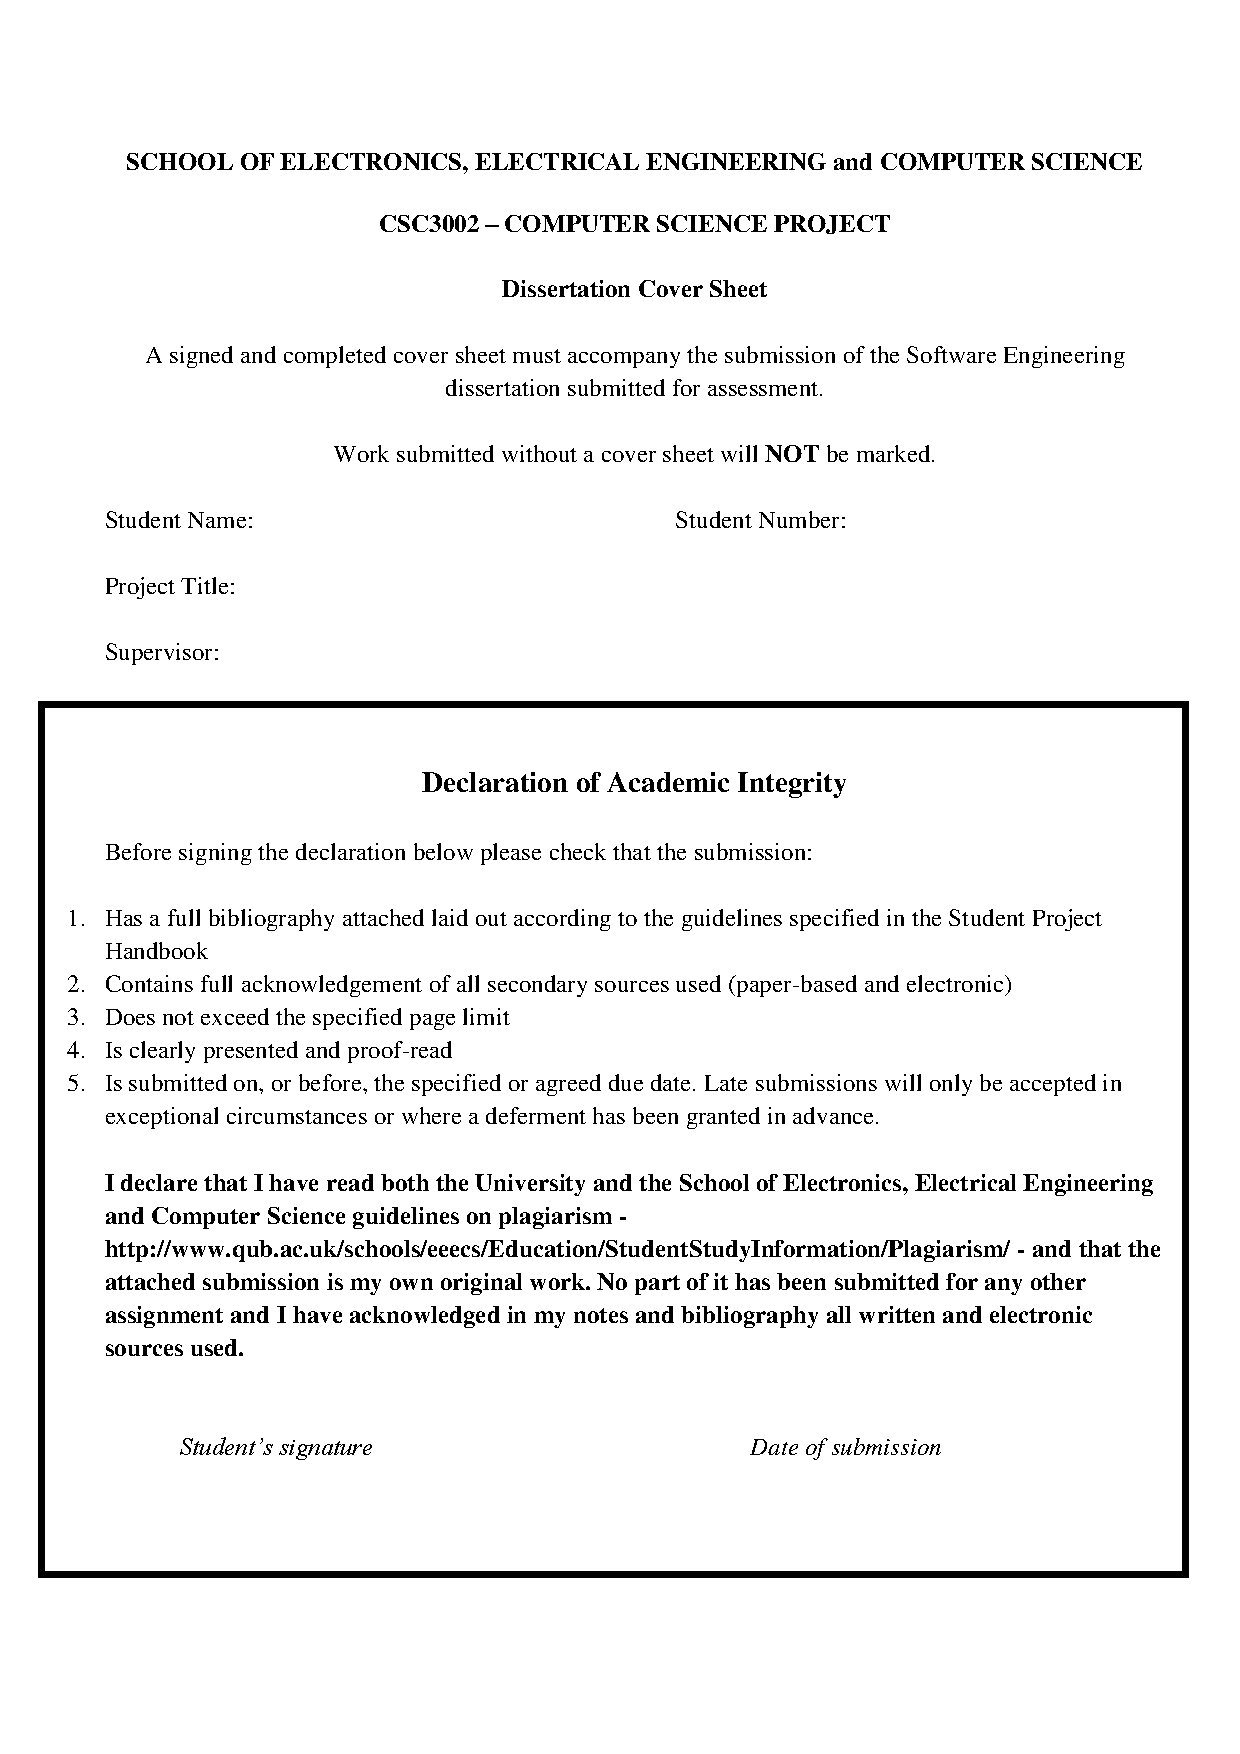
\includepdf{declaration.pdf}
I would like to thank my project supervisor, Dr. Cassio Polpo de Campos, for all of his guidance
and support during this project.

I’d also like to thank Queens University Belfast for assigning me a project that was of great
interest to me, and also for the usage of their facilities during this time.

I’d also like to thank my family for their support, and more importantly the refreshments
which they prepared.
% abstract.tex
\newpage
\begin{abstract}
Data used in the real world has a tendency to be incomplete, with values missing due to problems ranging from clerical error to data corruption. This dissertation is concerned with investigating the effects of repeatedly filling in missing values in training data, and especially by doing so using probabilistic methods. The accuracy of using models trained this way is then compared with models trained against the original data set, including the missing values. The accuracy of the implemented method is generally worse than using models which were trained against data sets with missing data, and therefore does not appear useful.
\end{abstract}
\tableofcontents
\listoftables
\listoffigures
% intro.tex
% Too short probably, maybe more background and some citations
\newpage
\chapter{Introduction}\label{intro}
The reliability of a machine learning model is heavily dependent on the data which was used to train it. Training data sets with missing values are therefore an interesting problem since there is no way of knowing what any given missing value could have been, and so the only two useful approaches involve either making statistical approximations of missing values or ignoring any record which contains missing data. Both mentioned approaches have positives as well as negatives. Ignoring a record prevents the use of unreliable data, but also may lead to valuable data in the other, non-missing attributes of the same record being discounted. The process of attempting to fill in a missing value is known as \textit{imputation}. This has no guarantee of being correct, but it may be worth the risk to gain value from the other complete attributes.  Using either approach may produce false outcomes. It is therefore extremely important that any imputation is carried out with care, and it must be very likely to be correct.

This project aims to investigate the usage of machine learning techniques on incomplete sets of discrete data. It will attempt to impute any missing values in the training data, by iteratively building and applying models until no further change is observed. It is expected that predicted missing values will trend towards the mean, leading to more reliable classification when this trained model is then applied to target data.  Given sufficient time, it is also intended that this approach can be used to infer 'hidden variables', similarly to how neural networks produce hidden layers to create relationships between data \cite{Touretzky:1989}. This will be achieved by adding a new attribute to a data set, and initially filling it full of random valid data. We will then repeatedly build, apply and rebuild models to classify this attribute until it stops changing, in an identical manner to how missing data is imputed in the training set. New data will be added to the training data set by this method, and this project aims to determine whether or not these hidden variables lead to a greater classification accuracy. All implemented code for this project, as well as some additional utility material, can be found at \cite{gitlab}.

% requirements.tex

The goal of this project is to study the effects of iteratively building common classifiers and comparing the performance of classifiers built this way against the performance of the same classifier, but without attempting to impute missing training data. The main aims of the software to be developed will therefore be:

\begin{itemize}
\item A Weka plugin will be developed. This should integrate smoothly into any version of Weka \textgreater  3.7.1, and will be made freely available. 
\item The classifier developed within the plugin should be usable from both the CLI and GUI.
\item Running experiments using the plugin should be easy, and have well explained documentation.
\item Allow any Weka classifier which is valid to use for a given dataset to be used within the newly implemented classifier, and for this to be easily configurable.
\item Run a number of experiments to compare the performance of the iteratively trained classifier against some control cases on the same data sets.
\end{itemize}

% design_implementation.tex
\newpage
\chapter{Design and Implementation}\label{design_impl}
\section{Design}
\label{design}
This body of work is mainly interested in popular classification algorithms, and in trying to use them in a slightly unusual way. It therefore makes sense to extend a package in which these are already implemented, and in which they are easily accessible. The Weka project~\cite{weka} suits this purpose since it has well maintained, efficient implementations of most machine learning algorithms, handles file I/O, and has both command line and graphical user interfaces. Since Weka is written in Java, it follows that the plugin should also be written in Java.

It also follows that any files which are used for testing should be in either .csv, or .arff format. The former is commonly used in data processing while the latter is a proprietary Weka format which is very similar, but differs in that it contains additional data at the top of the file pertaining to the data set. Both are supported by Weka, and therefore either is usable.

Since the project relies upon the idea that predictions for missing training data values should converge, it is assumed that the developed classifier will initially only work on nominal data sets. This is because nominal data sets should eventually settle on concrete values (at least when imputed using probabilistic techniques), whilst numeric values are not guaranteed to every settle on a particular value at all. It is more likely that numeric predictions would just change less and less between iterations, until the changes were minuscule. While it would be possible to implement a solution which stops iterating once a numeric data set only changes to a certain degree, as a proof of concept it is sensible to stick to nominal data.

It is intended that the implemented algorithm will work as follows:
\begin{enumerate}
\item Take a given training set, and make a copy of it
\item Fill the copy set with random, viable values
\item Use the produced data set to train a new model
\item Use the newly trained model to impute values into a new copy of the training set
\item Repeat 3 and 4 until identical data sets are produced by two consecutive iterations
\item Use the model built by the final iteration for classification of a test set
\end{enumerate}

\section{Implementation}
As an existing piece of software is being extended, much of the work to implement the various classifiers to be tested is already done. The main aim of this work is to integrate successfully into Weka as a plugin, and to interface with it as necessary. This plugin will be provided as a zip file containing the implemented algorithm which can be loaded by Weka using its package manager.
\subsection{Weka Architecture}
Weka is a Java package, with a source code layout which looks somewhat like this if unused packages are omitted: \\
\dirtree{%
.1 weka. 
.2 associations. 
.2 attributeSelection. 
.2 classifiers. 
.3 AbstractClassifier. 
.3 IterativeClassifier. 
.3 SingleClassifierEnhancer. 
.2 clusterers. 
.2 core. 
.3 Attribute. 
.3 Capabilities. 
.3 Instance. 
.3 Instances. 
.3 Option. 
.3 Utils. 
.2 datagenerators.
.2 estimators.
.2 experiment.
.2 filters.
.2 gui.
.2 knowledgeflow. }
\hfill \break
Each of these sub-packages is reasonably self explanatory. This project is mostly concerned with classifications, and thus code implemented for it lives in the \textit{weka.classifiers} package, although there are some dependencies on \textit{weka.core} since it contains much of the shared code for Weka. Provided that the rest of the project works as intended and the documentation is followed, there is no need to modify or discuss the other packages.

\subsection{weka.core}
From \textit{weka.core}, the following classes are used:

\begin{itemize}
\item \textbf{Attribute} - An Attribute in Weka refers to a single column in a data set. This object is mostly responsible for tracking the column's data type (e.g. nominal, numeric, etc), and other related information common to the entire column.
\item \textbf{Instance} - An Instance is the representation of a single row of data, roughly analogous to a row in a CSV file. Each Instance belongs to a particular Instances object. Each attribute value is stored as a Java double, which is then used in connection with an Attribute object to determine the actual value of an attribute.
\item \textbf{Instances} - An Instances object in Weka is used to represent a complete data set. It is roughly equivalent to the object representation of an ARFF file. It is comprised of a list of Instance objects,  a list of Attribute objects and some other metadata such as the class attribute for the data set and its name.
\item \textbf{Option} - An Option object represents a particular command line parameter, and the way in which it should be handled. This also contains a description to be printed in the help dialog if incorrect parameters are passed to the CLI.
\end{itemize}

\subsection{AbstractClassifier}
\textit{AbstractClassifier} is the class from which all classifiers which make nominal or numeric predictions in Weka are derived from. It provides a number of helpful implementations to prevent code duplication in classifiers, and to ease implementation. A pseudocode description of some notable methods can be seen below:

\begin{footnotesize}
\begin{verbatim}
abstract class AbstractClassifier {
    forName(classifierName, options) {
        return an instance of classifier <classifierName>
            with options <option>
    }

    runClassifier(classifier, options) {
        run any classifier by passing options to it
    }

    classifyInstance(instance) {
        returns the class which the instance is most 
            likely to belong to as a double in Weka's
            internal representation
    }

    distributionForInstance(instance) {
        return a list of probabilities for each 
            possible class value for a given instance
    }

    listOptions() {
        return all of the command line options which 
            a classifier accepts to configure how it will run
    }

    getOptions() {
        return the list of options which a classifier
            is currently set up to run with
    }

    setOptions(options) {
        sets the command line options for a
            classifier to options
    }

    getCapabilities() {
        returns a list of the attribute and class attribute 
            types which are supported by this classifier
    }
}
\end{verbatim}
\end{footnotesize}

There are a number of other utility and stub methods within this abstract class which may prove useful for other people in other cases, but have been omitted from the description above.

\subsection{SingleClassifierEnhancer}
\textit{SingleClassifierEnhancer} is a concrete class which extends from \textit{AbstractClassifier}, and from which the implemented ProjectClassifier extends. Extending from this class gives us a couple of benefits:
\begin{itemize}
\item \textit{SingleClassifierEnhancer} is designed for 'meta' classifiers, or those which wrap another classifier. It already contains an internal classifier and handles passing options to it. This can easily be extended to copy this classifier multiple times with the same options.
\item The internal classifier is already displayed nicely in the Weka GUI. This allows it to be configured via a menu, as shown in figure \ref{project_classifier_gui}.
\item It already handles some edge cases, such as calling the \textit{preExecution()} and \textit{postExecution()} methods of the internal classifier, which handles any specific setup and cleanup needed. These are small edge cases that would be easy to forget about, so extending in this way improves reliability by removing some of the mental overhead of the implementation.
\end{itemize}

\subsection{IterativeClassifier}
\textit{IterativeClassifier} is an Interface which is provided by Weka for 'classifiers which build models of increasing complexity'. It provides three method signatures: 
\begin{footnotesize}
\begin{verbatim}
public initializeClassifier() {
    do setup for the classifier
}

public next() {
    increase in complexity by one step by retraining the model
    return false if finished, or true if another step can be taken
}

public done() {
    stop increasing complexity and do any necessary cleanup
}
\end{verbatim}
\end{footnotesize}
These methods generally come together in the following pattern in a classifier which implements the interface:
\begin{footnotesize}
\begin{verbatim}
public buildClassifier(instances) {
    // some code here 
    initializeClassifier(instances)
    while(next()) {}
    done()
    // some other code here
}
\end{verbatim}
\end{footnotesize}
This means that building the classifier continues until it no longer makes sense to keep doing so, or no gain is achieved. This suits the project's use case, and therefore the interface makes sense to use.

\subsection{Weka Interfaces}
Calling a Weka classifier from the command line (assuming that the Weka jar file is already on the classpath) is reasonably straightforward. The target classifier is firstly called by its full path e.g.  \textit{java weka.classifiers.trees.J48}. Anything which comes after this point is passed to the classifier as an Option object. These are used as parameters to configure the behaviour of a particular classifier, and each class which extends from \textit{AbstractClassifier} generally implements its own specific set of Options through a combination of private variables and specifically named methods. The GUI appears works in much the same way, except that it provides windows with dropdown menus and text fields to allow classifiers and their Options to be configured.  

For example, imagine a given classifier had a private variable named \textit{m\_Example}. In order to expose this to the GUI and CLI it would require getter and setter methods, as well as an \textit{exampleTipText()} method to display help text. Code specifying how to handle this Option would also need to be added to the \textit{getOptions()}, \textit{setOptions()} and \textit{listOptions()} methods. 

\subsection{StateAnalyser}
The \textit{StateAnalyser} class has been designed to track the progress of the \textit{ProjectClassifier} as it is being trained. It contains a list of the training sets which have been produced by the \textit{next()} method, and records the number of differences between them. All of the methods described below are just utility methods for working with or comparing the training sets which have been produced.

\begin{footnotesize}
\begin{verbatim}
private convertToMatrix(instances) {
    create a matrix
    for each row in the data set {
        turn it into an array of floats
        add that array to the matrix
    }
    return matrix
}

public getNumberDifferences() {
    if at least two training sets recorded {
        convert the two most recent training sets to matrices
        for each row in both matrices {
            if the two rows differ, increment the difference counter
        }

        return the number of different rows;
    }

    else
        return a negative number to indicate an invalid test;
}


public getNumberIterations() {
    return number of recorded sets
}
\end{verbatim}
\end{footnotesize}
\subsection{ProjectClassifier}
\label{project_class}
The \textit{ProjectClassifier} class is the implementation of the algorithm described in section \ref{design}. This extends from \textit{SingleClassifierEnhancer} and implements the \textit{IterativeClassifier} interface. It maintains an internal array of classifiers, one for each of the attributes in a data set, and uses these to impute values into the training set as well as to classify test data. It also maintains three copies of training set while building:

\begin{itemize}
\item \textit{original} - a copy of the training set
\item \textit{last} - the last data set produced by imputing missing values, which can be used for retraining during the next iteration
\item \textit{current} - the data set which is currently having its missing values filled in
\end{itemize}

\begin{footnotesize}
\begin{verbatim}
public buildClassifier(instances) {
    record the index of the original class attribute
    take a reference copy of the training set (original)
    find the location of missing data in the training set
    set up the classifier for the first run
    repeat until no change is observed between current and last
    perform any cleanup needed
}

public findMissingAttributes(instances) {
    for each instance in a training set {
        record any values which are missing for later use
    }
}

public initializeClassifier(instances) {
    create new tracker object
    create one classifier object per attribute in the data set
    take two modifiable copies of the training data set (last/current)
    replace any missing data in last using random values
}

public replaceMissingValues(instances) {
    for any each piece of missing data {
        input a random possible value
    }
}

public next() {
    replace last with current
    replace current with a new copy of the training data
    retrain classifiers against last
    for each recorded missing value {
        use trained classifiers to impute missing values in current
    }
    add current to the tracker object
    if (there are no differences between current and last)
        stop iterating
    else   
        iterate again
}

public done() {
    do option specific cleanup
}

public retrainClassifiers(instances) {
    for each attribute in the training set {
        retrain a classifier against that attribute
    }
}
\end{verbatim}
\end{footnotesize}

\textit{ProjectClassifier} also accepts some options, which can be used to configure how it runs:
\begin{itemize}
\item \textbf{maxIterations} (-M number) - Some classifiers may not converge in the way in which we expect, or they make take a very long time to reach this point. This flag allows for a maximum number of training iterations to be set in order to ensure experiments finish in a timely fashion.
\item \textbf{supervised} (-S) - It may be interesting to observe the difference between classifiers which are trained against a training set where the class attribute is trained iteratively along with the rest of the data set against a training set where missing class attribute values are not imputed until the classifier rest of the classifier has converged. This flag allows for the latter case to be tested.
\item \textbf{randomData} (-R) - As a control set during experiments, it make sense to fill a training set with random data and determine whether or not the implemented algorithm outperforms classifiers which are trained against this. This allows this experiment to be performed.
\item \textbf{hiddenVariables} (-N) - See appendix \ref{hidden}.
\end{itemize}

\subsection{Testing}

Unit tests were written for both the \textit{StateAnalyser} and \textit{ProjectClassifier} classes using JUnit 3 since Weka's unit tests are written using this version. While JUnit 4 and 5 are both available, it seems sensible to use the same version for both as there are large changes in how tests are defined and written between versions. These tests allowed for reasonably quick iteration, and in the case of the \textit{ProjectClassifier} class provided useful debugging information.

Unfortunately more rigorous testing could not be performed due to the nature of this work. Since this is an experimental implementation, the expected results are unknown and are therefore only testable through experimentation as described in section \ref{experiments}.
% experiments.tex
\newpage
\chapter{Experiments}\label{experiments}
The algorithm described in the previous section will be used in experiments with a number of internal classifiers in order to assess their performance when trained iteratively. These results will be compared with the results of using the internal classifier in a number of control cases, to determine if the implemented algorithm described has proven beneficial. Each case will be tested against 51 different sets of nominal data taken from the UCI Machine Learning Repository~\cite{Lichman:2013}, each of which has had approximately 10\% of its values removed at random in order to simulate the effects of having missing data. For each data set, 5 folds will be used for cross validation and this will be repeated 10 times. Additional information about the data sets can be found in appendix \ref{datasets}.

For each classifier which we are testing we will use the following test cases, where \textit{TestClassifier} represents the current classifier under test:

\begin{enumerate}
\item \textit{ProjectClassifier -S with TestClassifier} - Iteratively trains the target classifier by imputing missing values, retraining against the newly completed data set and then imputing again until convergence or max iterations reached. The class attribute is not guessed.
\item \textit{ProjectClassifier with TestClassifier} - Same as previous case, except that the initial class attribute is also iteratively imputed.
\item \textit{TestClassifier} - 'Vanilla' classifier, run without attempting to remove missing values before classification.
\item \textit{TestClassifier (missing data filled in with mode)} - Same as previous case, except every missing value will be replaced using the mode before it is run.
\item \textit{ProjectClassifier -R with TestClassifier} - Similar to previous case, except missing values will be replaced using random possible values before classification. Only one iteration will be performed.
\end{enumerate}

Each of these tests will henceforth be referred to as Case 1, 2, 3, 4 and 5 respectively. For each of the tables discussed below, the index of each column refers to the number of each case. 

Some adaptations may need to be made for certain classifiers, but this is the general structure of each experiment. For each of these classifiers the percentage of incorrect classifications, mean absolute error (MAE), root mean squared error (RMSE), and mean entropy gain (MEG) will be compared using a paired T test with a statistical significance threshold of 0.05. It is generally expected that Case 1, the iteratively trained classifier, will perform better than all other cases with the possible exception of Case 3.

\section{Results}

Tables referenced below can be found at the end of each subsection, since they are too large to be included in-line.

\subsection{Naive Bayes}
No adaptations needed to be made for the Naive Bayes classification method since it converged to a stable model as expected, and did so within a reasonable period of time.

Naive Bayes Percent Incorrect results are shown in Table \ref{nbpi}. As expected, Case 1 generally performed better than Cases 2, 4 and 5. It seems logical that Cases 4 and 5 would perform the worst, since these methods generally just involved filling in missing data with the most common and random data respectively. Case 1 generally performed worse than Case 3, producing statistically even results in 30 tests and statistically worse results in 19 tests.

Naive Bayes MAE results are shown in Table \ref{nbmae}. Cases 1, 2 and 3 proved approximately equal according to this test, with no real significant difference between results. Case 1 performed much better than Cases 4 or 5, showing better results in 37 and 45 tests respectively. This is an expected result, since Cases 4 and 5 are effectively control cases.

Naive Bayes RMSE results are shown in Table \ref{nbrmse}. Using this metric for measurement, Case 1 performed significantly better than both Cases 2 and 4, with better results shown in 41 and 28 data sets respectively. Interestingly, it performed about as well as Case 5, performing significantly better in 17 tests, approximately about as well in 16 tests, and significantly worse in 18 tests. This could be due to the fact that using random data is unlikely to lead to strong predictions being made, while iteratively imputing missing values will tend to result in either increasingly bad or increasingly good predictions being made. Again, Case 3 performed significantly better than Case 1.

Naive Bayes MEG results are shown in Table \ref{nbmeg}. Case 1 performed significantly worse than Case 2 according to this metric, performing worse in 42/51 data sets. It is assumed that this is due to the iterative imputation of the class attribute in Case 2, which probably leads to lower entropy gains since it will produce a smaller range of values. For a very similar reason, Case 1 performs significantly better than Case 3. Since it's iteratively imputing all but one attribute in the training set, a smaller range of values are probably produced during classification. Cases 1, 4 and 5 perform about as well as each other, since Cases 4 and 5 are essentially just making random guesses.

It would seem that the implemented algorithm does not provide any significant gains when using the Naive Bayes classifier according to the measurements used. While significant decreases in entropy gain were observed, it was both less accurate as a classifier and more strongly wrong.

\newpage
{\centering \footnotesize \begin{longtable}{lrr@{\hspace{0.1cm}}cr@{\hspace{0.1cm}}cr@{\hspace{0.1cm}}cr@{\hspace{0.1cm}}c}
\caption{\label{nbpi}Naive Bayes Percent Incorrect}\\
\hline
Dataset & (1)& (2) & & (3) & & (4) & & (5) & \\
\hline
audiology & 36.33 & 38.44 &   $\circ$ & 37.28 &   $\circ$ & 50.09 &    $\circ$ & 43.50 &    $\circ$\\
autos & 10.33 &  9.78 & $\bullet$ & 10.22 &           &  9.62 &  $\bullet$ &  9.61 &  $\bullet$\\
balance-scale & 26.54 & 25.96 & $\bullet$ & 26.26 & $\bullet$ & 28.49 &    $\circ$ & 25.98 &  $\bullet$\\
breast-cancer & 27.67 & 27.63 &           & 27.14 &           & 27.41 &            & 27.33 &           \\
bridges-version1 & 35.44 & 33.67 & $\bullet$ & 35.45 &           & 36.00 &            & 38.04 &    $\circ$\\
car & 19.26 & 19.67 &   $\circ$ & 19.46 &           & 23.23 &    $\circ$ & 21.39 &    $\circ$\\
cmc & 51.80 & 52.27 &   $\circ$ & 50.69 & $\bullet$ & 50.24 &  $\bullet$ & 51.24 &  $\bullet$\\
colic & 21.45 & 21.94 &           & 20.92 & $\bullet$ & 19.94 &  $\bullet$ & 21.72 &           \\
cylinder-bands & 32.26 & 33.12 &   $\circ$ & 31.79 & $\bullet$ & 32.69 &            & 32.92 &           \\
dermatology &  3.19 &  3.04 &           &  2.95 &           &  3.58 &            &  3.31 &           \\
diabetes & 28.12 & 28.90 &   $\circ$ & 27.79 &           & 27.52 &            & 28.41 &           \\
ecoli & 33.61 & 33.52 &           & 32.67 & $\bullet$ & 34.53 &    $\circ$ & 32.44 &  $\bullet$\\
flags & 37.83 & 37.60 &           & 38.46 &           & 40.51 &    $\circ$ & 39.77 &    $\circ$\\
glass & 45.98 & 44.97 &           & 46.42 &           & 46.58 &            & 46.02 &           \\
haberman & 28.30 & 28.12 &           & 27.71 &           & 27.27 &  $\bullet$ & 27.31 &  $\bullet$\\
hayes-roth-train & 51.28 & 52.26 &           & 47.16 & $\bullet$ & 49.23 &            & 50.26 &           \\
heart-h & 17.98 & 18.05 &           & 18.39 &           & 19.23 &    $\circ$ & 18.24 &           \\
heart-statlog & 27.15 & 27.15 &           & 27.10 &           & 27.51 &            & 27.03 &           \\
hepatitis & 18.98 & 19.05 &           & 19.06 &           & 19.20 &            & 19.35 &           \\
hypothyroid &  9.14 & 12.42 &   $\circ$ &  8.74 & $\bullet$ &  8.38 &  $\bullet$ &  7.76 &  $\bullet$\\
ionosphere & 27.11 & 30.89 &   $\circ$ & 24.93 & $\bullet$ & 23.94 &  $\bullet$ & 25.97 &  $\bullet$\\
iris & 21.29 & 21.59 &           & 21.51 &           & 23.54 &    $\circ$ & 22.26 &           \\
kr-vs-kp & 14.69 & 16.55 &   $\circ$ & 14.01 & $\bullet$ & 16.69 &    $\circ$ & 16.31 &    $\circ$\\
labor &  5.40 &  5.00 &           &  4.80 &           &  5.20 &            &  7.00 &    $\circ$\\
letter & 60.44 & 61.98 &   $\circ$ & 59.84 & $\bullet$ & 62.59 &    $\circ$ & 60.33 &  $\bullet$\\
liver-disorders & 38.00 & 39.84 &   $\circ$ & 37.31 &           & 39.17 &            & 37.99 &           \\
lung-cancer & 49.89 & 47.90 &           & 53.02 &           & 45.55 &            & 53.19 &           \\
lymph & 16.60 & 16.30 &           & 15.65 & $\bullet$ & 16.49 &            & 16.65 &           \\
molecular-biology-promoters &  9.73 & 10.18 &           &  8.56 &           & 14.00 &    $\circ$ & 10.39 &           \\
mushroom &  5.06 &  6.86 &   $\circ$ &  5.06 &           &  7.89 &    $\circ$ &  8.06 &    $\circ$\\
nursery & 16.01 & 16.08 &           & 15.87 &           & 16.51 &    $\circ$ & 15.63 &  $\bullet$\\
optdigits & 13.60 & 14.06 &   $\circ$ & 13.10 & $\bullet$ & 16.32 &    $\circ$ & 14.55 &    $\circ$\\
page-blocks & 16.82 & 19.30 &   $\circ$ & 16.82 &           & 14.00 &  $\bullet$ &  9.17 &  $\bullet$\\
pendigits & 21.97 & 22.49 &   $\circ$ & 21.21 & $\bullet$ & 26.14 &    $\circ$ & 23.08 &    $\circ$\\
postoperative-patient-data & 30.69 & 31.41 &           & 29.98 &           & 30.36 &            & 33.26 &    $\circ$\\
primary-tumor & 54.72 & 55.26 &           & 54.13 &           & 54.94 &            & 56.04 &    $\circ$\\
segment & 28.72 & 30.80 &   $\circ$ & 28.12 & $\bullet$ & 33.04 &    $\circ$ & 31.49 &    $\circ$\\
shuttle-landing-control & 44.00 & 42.67 &           & 46.67 &           & 36.67 &  $\bullet$ & 45.33 &           \\
sick &  9.64 & 10.26 &   $\circ$ &  9.81 &   $\circ$ &  8.84 &  $\bullet$ &  7.98 &  $\bullet$\\
solar-flare-2 & 28.23 & 28.22 &           & 28.16 &           & 28.39 &            & 28.21 &           \\
sonar & 24.86 & 26.31 &   $\circ$ & 24.14 & $\bullet$ & 25.33 &            & 24.60 &           \\
soybean &  9.62 & 10.51 &   $\circ$ &  9.77 &           & 11.28 &    $\circ$ & 11.91 &    $\circ$\\
spambase & 24.61 & 24.85 &   $\circ$ & 24.51 & $\bullet$ & 24.14 &  $\bullet$ & 24.57 &           \\
tae & 49.72 & 50.00 &           & 48.92 &           & 51.64 &    $\circ$ & 51.37 &    $\circ$\\
tic-tac-toe & 30.03 & 30.21 &           & 29.49 & $\bullet$ & 29.23 &  $\bullet$ & 29.33 &  $\bullet$\\
trains & 33.00 & 33.00 &           & 31.00 &           & 39.00 &            & 33.00 &           \\
vehicle & 55.02 & 56.60 &   $\circ$ & 53.71 & $\bullet$ & 55.79 &    $\circ$ & 54.53 &           \\
vote &  9.47 &  9.57 &   $\circ$ &  9.47 &           &  9.34 &            &  9.64 &           \\
vowel & 70.35 & 71.30 &   $\circ$ & 69.27 & $\bullet$ & 72.30 &    $\circ$ & 69.72 &           \\
waveform-5000 & 22.34 & 22.65 &   $\circ$ & 22.44 &           & 23.63 &    $\circ$ & 23.04 &    $\circ$\\
zoo &  8.99 &  9.86 &   $\circ$ &  8.78 &           & 11.33 &    $\circ$ & 11.16 &    $\circ$\\
\hline
Average & 27.71 & 28.24 &           & 27.37 &           & 28.52 &            & 28.18 &           \\
\hline
\multicolumn{10}{c}{$\circ$, $\bullet$ statistically significant improvement or degradation}\\
\end{longtable} \footnotesize \par}

\begin{table}[H]
\caption{\label{nbmae}Naive Bayes MAE}
\footnotesize
{\centering \begin{tabular}{lrr@{\hspace{0.1cm}}cr@{\hspace{0.1cm}}cr@{\hspace{0.1cm}}cr@{\hspace{0.1cm}}c}
\\
\hline
Dataset & (1)& (2) & & (3) & & (4) & & (5) & \\
\hline
audiology & 0.03 & 0.03 &    $\circ$ & 0.03 &    $\circ$ & 0.04 &   $\circ$ & 0.04 &   $\circ$\\
autos & 0.10 & 0.10 &  $\bullet$ & 0.10 &  $\bullet$ & 0.10 &           & 0.10 &          \\
balance-scale & 0.25 & 0.25 &  $\bullet$ & 0.27 &    $\circ$ & 0.28 &   $\circ$ & 0.29 &   $\circ$\\
breast-cancer & 0.33 & 0.32 &  $\bullet$ & 0.32 &            & 0.32 &           & 0.34 &   $\circ$\\
bridges-version1 & 0.15 & 0.14 &  $\bullet$ & 0.15 &    $\circ$ & 0.15 &   $\circ$ & 0.16 &   $\circ$\\
car & 0.13 & 0.13 &  $\bullet$ & 0.13 &    $\circ$ & 0.14 &   $\circ$ & 0.17 &   $\circ$\\
cmc & 0.38 & 0.38 &  $\bullet$ & 0.38 &    $\circ$ & 0.39 &   $\circ$ & 0.39 &   $\circ$\\
colic & 0.23 & 0.24 &    $\circ$ & 0.23 &  $\bullet$ & 0.22 & $\bullet$ & 0.25 &   $\circ$\\
cylinder-bands & 0.35 & 0.35 &    $\circ$ & 0.34 &            & 0.35 &           & 0.37 &   $\circ$\\
dermatology & 0.01 & 0.01 &  $\bullet$ & 0.01 &  $\bullet$ & 0.02 &   $\circ$ & 0.02 &   $\circ$\\
diabetes & 0.33 & 0.33 &    $\circ$ & 0.33 &    $\circ$ & 0.33 &   $\circ$ & 0.35 &   $\circ$\\
ecoli & 0.10 & 0.10 &  $\bullet$ & 0.10 &    $\circ$ & 0.11 &   $\circ$ & 0.11 &   $\circ$\\
flags & 0.10 & 0.10 &            & 0.10 &    $\circ$ & 0.11 &   $\circ$ & 0.11 &   $\circ$\\
glass & 0.16 & 0.16 &  $\bullet$ & 0.16 &    $\circ$ & 0.16 &   $\circ$ & 0.17 &   $\circ$\\
haberman & 0.37 & 0.36 &  $\bullet$ & 0.37 &            & 0.37 & $\bullet$ & 0.39 &   $\circ$\\
hayes-roth-train & 0.31 & 0.31 &            & 0.31 &            & 0.31 &   $\circ$ & 0.32 &   $\circ$\\
heart-h & 0.09 & 0.09 &  $\bullet$ & 0.09 &    $\circ$ & 0.10 &   $\circ$ & 0.11 &   $\circ$\\
heart-statlog & 0.30 & 0.29 &            & 0.30 &    $\circ$ & 0.31 &   $\circ$ & 0.31 &   $\circ$\\
hepatitis & 0.21 & 0.21 &            & 0.21 &    $\circ$ & 0.21 &   $\circ$ & 0.23 &   $\circ$\\
hypothyroid & 0.07 & 0.08 &    $\circ$ & 0.07 &  $\bullet$ & 0.07 & $\bullet$ & 0.10 &   $\circ$\\
ionosphere & 0.28 & 0.31 &    $\circ$ & 0.26 &  $\bullet$ & 0.26 & $\bullet$ & 0.28 &          \\
iris & 0.18 & 0.17 &  $\bullet$ & 0.18 &            & 0.21 &   $\circ$ & 0.20 &   $\circ$\\
kr-vs-kp & 0.23 & 0.24 &    $\circ$ & 0.23 &  $\bullet$ & 0.25 &   $\circ$ & 0.29 &   $\circ$\\
labor & 0.08 & 0.08 &            & 0.08 &            & 0.09 &   $\circ$ & 0.11 &   $\circ$\\
letter & 0.05 & 0.05 &  $\bullet$ & 0.05 &  $\bullet$ & 0.06 &   $\circ$ & 0.06 &   $\circ$\\
liver-disorders & 0.46 & 0.46 &            & 0.46 &            & 0.46 &           & 0.47 &   $\circ$\\
lung-cancer & 0.34 & 0.33 &            & 0.36 &    $\circ$ & 0.31 & $\bullet$ & 0.35 &          \\
lymph & 0.10 & 0.10 &    $\circ$ & 0.10 &            & 0.11 &   $\circ$ & 0.11 &   $\circ$\\
molecular-biology-promoters & 0.11 & 0.12 &    $\circ$ & 0.11 &            & 0.15 &   $\circ$ & 0.13 &   $\circ$\\
mushroom & 0.05 & 0.07 &    $\circ$ & 0.05 &  $\bullet$ & 0.08 &   $\circ$ & 0.08 &   $\circ$\\
nursery & 0.09 & 0.09 &  $\bullet$ & 0.10 &    $\circ$ & 0.13 &   $\circ$ & 0.14 &   $\circ$\\
optdigits & 0.03 & 0.03 &    $\circ$ & 0.03 &  $\bullet$ & 0.04 &   $\circ$ & 0.04 &   $\circ$\\
page-blocks & 0.08 & 0.09 &    $\circ$ & 0.08 &  $\bullet$ & 0.07 & $\bullet$ & 0.10 &   $\circ$\\
pendigits & 0.05 & 0.05 &  $\bullet$ & 0.05 &  $\bullet$ & 0.07 &   $\circ$ & 0.06 &   $\circ$\\
postoperative-patient-data & 0.28 & 0.28 &    $\circ$ & 0.28 &    $\circ$ & 0.27 & $\bullet$ & 0.30 &   $\circ$\\
primary-tumor & 0.06 & 0.06 &  $\bullet$ & 0.06 &            & 0.06 &   $\circ$ & 0.06 &   $\circ$\\
segment & 0.09 & 0.10 &    $\circ$ & 0.09 &  $\bullet$ & 0.11 &   $\circ$ & 0.11 &   $\circ$\\
shuttle-landing-control & 0.46 & 0.45 &            & 0.46 &            & 0.44 & $\bullet$ & 0.47 &   $\circ$\\
sick & 0.12 & 0.12 &    $\circ$ & 0.12 &    $\circ$ & 0.11 & $\bullet$ & 0.16 &   $\circ$\\
solar-flare-2 & 0.11 & 0.11 &  $\bullet$ & 0.11 &    $\circ$ & 0.12 &   $\circ$ & 0.13 &   $\circ$\\
sonar & 0.25 & 0.26 &    $\circ$ & 0.25 &  $\bullet$ & 0.26 &   $\circ$ & 0.25 & $\bullet$\\
soybean & 0.01 & 0.01 &    $\circ$ & 0.01 &            & 0.01 &   $\circ$ & 0.02 &   $\circ$\\
spambase & 0.27 & 0.27 &    $\circ$ & 0.27 &    $\circ$ & 0.28 &   $\circ$ & 0.29 &   $\circ$\\
tae & 0.40 & 0.40 &            & 0.40 &    $\circ$ & 0.41 &   $\circ$ & 0.41 &   $\circ$\\
tic-tac-toe & 0.36 & 0.36 &  $\bullet$ & 0.37 &    $\circ$ & 0.37 &   $\circ$ & 0.39 &   $\circ$\\
trains & 0.32 & 0.35 &            & 0.33 &            & 0.35 &           & 0.33 &          \\
vehicle & 0.29 & 0.29 &    $\circ$ & 0.28 &  $\bullet$ & 0.29 &   $\circ$ & 0.29 &          \\
vote & 0.10 & 0.10 &    $\circ$ & 0.10 &  $\bullet$ & 0.10 &   $\circ$ & 0.10 &   $\circ$\\
vowel & 0.14 & 0.14 &    $\circ$ & 0.14 &  $\bullet$ & 0.15 &   $\circ$ & 0.14 &   $\circ$\\
waveform-5000 & 0.16 & 0.16 &    $\circ$ & 0.16 &  $\bullet$ & 0.17 &   $\circ$ & 0.17 &   $\circ$\\
zoo & 0.03 & 0.03 &            & 0.03 &            & 0.04 &   $\circ$ & 0.04 &   $\circ$\\
\hline
Average & 0.19 & 0.19 &            & 0.19 &            & 0.20 &           & 0.20 &          \\
\hline
\multicolumn{10}{c}{$\circ$, $\bullet$ statistically significant improvement or degradation}\\
\end{tabular} \footnotesize \par}
\end{table}

\begin{table}[htb]
\caption{\label{nbrmse}Naive Bayes Root Mean Squared Error}
\footnotesize
{\centering \begin{tabular}{lrr@{\hspace{0.1cm}}cr@{\hspace{0.1cm}}cr@{\hspace{0.1cm}}cr@{\hspace{0.1cm}}c}
\\
\hline
Dataset & (1)& (2) & & (3) & & (4) & & (5) & \\
\hline
audiology & 0.16 & 0.16 &   $\circ$ & 0.16 &   $\circ$ & 0.17 &   $\circ$ & 0.16 &    $\circ$\\
autos & 0.29 & 0.28 & $\bullet$ & 0.28 & $\bullet$ & 0.27 & $\bullet$ & 0.28 &  $\bullet$\\
balance-scale & 0.34 & 0.34 &   $\circ$ & 0.34 &   $\circ$ & 0.36 &   $\circ$ & 0.35 &    $\circ$\\
breast-cancer & 0.45 & 0.45 &   $\circ$ & 0.45 & $\bullet$ & 0.44 & $\bullet$ & 0.44 &  $\bullet$\\
bridges-version1 & 0.28 & 0.29 &           & 0.28 &           & 0.29 &   $\circ$ & 0.29 &    $\circ$\\
car & 0.24 & 0.24 &   $\circ$ & 0.25 &   $\circ$ & 0.26 &   $\circ$ & 0.27 &    $\circ$\\
cmc & 0.46 & 0.47 &   $\circ$ & 0.46 & $\bullet$ & 0.45 & $\bullet$ & 0.45 &  $\bullet$\\
colic & 0.42 & 0.43 &   $\circ$ & 0.41 & $\bullet$ & 0.41 & $\bullet$ & 0.41 &  $\bullet$\\
cylinder-bands & 0.47 & 0.49 &   $\circ$ & 0.47 & $\bullet$ & 0.47 & $\bullet$ & 0.46 &  $\bullet$\\
dermatology & 0.08 & 0.08 &           & 0.08 & $\bullet$ & 0.09 &   $\circ$ & 0.09 &    $\circ$\\
diabetes & 0.43 & 0.44 &   $\circ$ & 0.43 & $\bullet$ & 0.42 & $\bullet$ & 0.42 &  $\bullet$\\
ecoli & 0.23 & 0.23 &   $\circ$ & 0.23 & $\bullet$ & 0.23 &   $\circ$ & 0.23 &           \\
flags & 0.26 & 0.27 &   $\circ$ & 0.26 &           & 0.27 &   $\circ$ & 0.27 &           \\
glass & 0.29 & 0.29 &   $\circ$ & 0.29 & $\bullet$ & 0.29 &           & 0.29 &           \\
haberman & 0.44 & 0.44 &           & 0.44 & $\bullet$ & 0.44 &   $\circ$ & 0.44 &           \\
hayes-roth-train & 0.39 & 0.39 &   $\circ$ & 0.38 & $\bullet$ & 0.39 &   $\circ$ & 0.39 &    $\circ$\\
heart-h & 0.23 & 0.23 &   $\circ$ & 0.23 & $\bullet$ & 0.23 &   $\circ$ & 0.23 &           \\
heart-statlog & 0.43 & 0.44 &   $\circ$ & 0.43 & $\bullet$ & 0.42 & $\bullet$ & 0.42 &  $\bullet$\\
hepatitis & 0.39 & 0.39 &   $\circ$ & 0.39 &           & 0.39 &           & 0.38 &  $\bullet$\\
hypothyroid & 0.19 & 0.22 &   $\circ$ & 0.18 & $\bullet$ & 0.18 & $\bullet$ & 0.19 &    $\circ$\\
ionosphere & 0.45 & 0.50 &   $\circ$ & 0.44 & $\bullet$ & 0.43 & $\bullet$ & 0.44 &  $\bullet$\\
iris & 0.32 & 0.32 &           & 0.32 &           & 0.34 &   $\circ$ & 0.32 &    $\circ$\\
kr-vs-kp & 0.32 & 0.34 &   $\circ$ & 0.32 & $\bullet$ & 0.34 &   $\circ$ & 0.35 &    $\circ$\\
labor & 0.18 & 0.18 &           & 0.17 & $\bullet$ & 0.19 &           & 0.20 &    $\circ$\\
letter & 0.17 & 0.17 &   $\circ$ & 0.17 & $\bullet$ & 0.17 &   $\circ$ & 0.17 &  $\bullet$\\
liver-disorders & 0.48 & 0.49 &   $\circ$ & 0.48 & $\bullet$ & 0.48 &   $\circ$ & 0.48 &           \\
lung-cancer & 0.51 & 0.50 &           & 0.52 &           & 0.48 & $\bullet$ & 0.52 &           \\
lymph & 0.24 & 0.24 &   $\circ$ & 0.23 & $\bullet$ & 0.24 &           & 0.24 &           \\
molecular-biology-promoters & 0.24 & 0.26 &   $\circ$ & 0.24 &           & 0.31 &   $\circ$ & 0.26 &    $\circ$\\
mushroom & 0.20 & 0.25 &   $\circ$ & 0.20 & $\bullet$ & 0.26 &   $\circ$ & 0.26 &    $\circ$\\
nursery & 0.21 & 0.21 &   $\circ$ & 0.21 &   $\circ$ & 0.23 &   $\circ$ & 0.23 &    $\circ$\\
optdigits & 0.15 & 0.15 &   $\circ$ & 0.14 & $\bullet$ & 0.16 &   $\circ$ & 0.15 &           \\
page-blocks & 0.22 & 0.24 &   $\circ$ & 0.21 & $\bullet$ & 0.20 & $\bullet$ & 0.19 &  $\bullet$\\
pendigits & 0.18 & 0.18 &   $\circ$ & 0.18 & $\bullet$ & 0.20 &   $\circ$ & 0.18 &    $\circ$\\
postoperative-patient-data & 0.39 & 0.40 &   $\circ$ & 0.39 &           & 0.39 &           & 0.40 &           \\
primary-tumor & 0.18 & 0.18 &   $\circ$ & 0.18 & $\bullet$ & 0.18 &   $\circ$ & 0.18 &    $\circ$\\
segment & 0.25 & 0.25 &   $\circ$ & 0.24 & $\bullet$ & 0.26 &   $\circ$ & 0.25 &           \\
shuttle-landing-control & 0.49 & 0.49 &           & 0.49 &           & 0.48 & $\bullet$ & 0.50 &           \\
sick & 0.26 & 0.27 &   $\circ$ & 0.26 & $\bullet$ & 0.25 & $\bullet$ & 0.25 &  $\bullet$\\
solar-flare-2 & 0.24 & 0.25 &   $\circ$ & 0.24 & $\bullet$ & 0.25 &   $\circ$ & 0.25 &           \\
sonar & 0.45 & 0.46 &   $\circ$ & 0.44 & $\bullet$ & 0.45 &   $\circ$ & 0.43 &  $\bullet$\\
soybean & 0.09 & 0.10 &   $\circ$ & 0.09 &           & 0.10 &   $\circ$ & 0.10 &    $\circ$\\
spambase & 0.43 & 0.43 &   $\circ$ & 0.42 & $\bullet$ & 0.42 & $\bullet$ & 0.41 &  $\bullet$\\
tae & 0.46 & 0.46 &   $\circ$ & 0.46 & $\bullet$ & 0.46 &           & 0.46 &           \\
tic-tac-toe & 0.44 & 0.44 &   $\circ$ & 0.43 & $\bullet$ & 0.44 &   $\circ$ & 0.44 &           \\
trains & 0.40 & 0.42 &           & 0.41 &           & 0.43 &           & 0.42 &           \\
vehicle & 0.45 & 0.46 &   $\circ$ & 0.44 & $\bullet$ & 0.44 & $\bullet$ & 0.43 &  $\bullet$\\
vote & 0.29 & 0.30 &   $\circ$ & 0.29 & $\bullet$ & 0.29 & $\bullet$ & 0.29 &  $\bullet$\\
vowel & 0.27 & 0.28 &   $\circ$ & 0.27 & $\bullet$ & 0.28 &   $\circ$ & 0.27 &  $\bullet$\\
waveform-5000 & 0.35 & 0.35 &   $\circ$ & 0.35 & $\bullet$ & 0.35 &   $\circ$ & 0.35 &  $\bullet$\\
zoo & 0.13 & 0.13 &           & 0.12 &           & 0.14 &   $\circ$ & 0.14 &    $\circ$\\
\hline
Average & 0.31 & 0.32 &           & 0.31 &           & 0.32 &           & 0.31 &           \\
\hline
\multicolumn{10}{c}{$\circ$, $\bullet$ statistically significant improvement or degradation}\\
\end{tabular} \footnotesize \par}
\end{table}

\begin{table}[htb]
\caption{\label{nbmeg}Naive Bayes Mean Entropy Gain}
\footnotesize
{\centering \begin{tabular}{lrr@{\hspace{0.1cm}}cr@{\hspace{0.1cm}}cr@{\hspace{0.1cm}}cr@{\hspace{0.1cm}}c}
\\
\hline
Dataset & (1)& (2) & & (3) & & (4) & & (5) & \\
\hline
audiology & -1.07 & -1.31 & $\bullet$ & -1.30 & $\bullet$ & -2.14 & $\bullet$ & -0.49 &    $\circ$\\
autos & -0.10 & -0.12 & $\bullet$ & -0.04 &   $\circ$ &  0.11 &   $\circ$ &  0.17 &    $\circ$\\
balance-scale &  0.42 &  0.41 & $\bullet$ &  0.39 & $\bullet$ &  0.32 & $\bullet$ &  0.35 &  $\bullet$\\
breast-cancer & -0.04 & -0.07 & $\bullet$ & -0.02 &   $\circ$ & -0.00 &   $\circ$ &  0.03 &    $\circ$\\
bridges-version1 &  0.73 &  0.68 & $\bullet$ &  0.75 &   $\circ$ &  0.67 & $\bullet$ &  0.72 &           \\
car &  0.65 &  0.65 & $\bullet$ &  0.63 & $\bullet$ &  0.57 & $\bullet$ &  0.45 &  $\bullet$\\
cmc &  0.01 & -0.08 & $\bullet$ &  0.04 &   $\circ$ &  0.04 &   $\circ$ &  0.08 &    $\circ$\\
colic & -0.32 & -0.43 & $\bullet$ & -0.22 &   $\circ$ & -0.17 &   $\circ$ &  0.01 &    $\circ$\\
cylinder-bands & -0.02 & -0.16 & $\bullet$ &  0.02 &   $\circ$ &  0.04 &   $\circ$ &  0.07 &    $\circ$\\
dermatology &  2.32 &  2.32 &           &  2.33 &   $\circ$ &  2.29 & $\bullet$ &  2.30 &  $\bullet$\\
diabetes &  0.14 &  0.12 & $\bullet$ &  0.16 &   $\circ$ &  0.16 &   $\circ$ &  0.17 &    $\circ$\\
ecoli &  0.98 &  0.96 & $\bullet$ &  1.00 &   $\circ$ &  0.96 &           &  0.95 &  $\bullet$\\
flags &  0.27 &  0.12 & $\bullet$ &  0.31 &   $\circ$ &  0.27 &           &  0.45 &    $\circ$\\
glass &  0.53 &  0.48 & $\bullet$ &  0.55 &   $\circ$ &  0.53 &           &  0.50 &           \\
haberman & -0.00 & -0.01 &           &  0.01 &   $\circ$ & -0.01 & $\bullet$ &  0.01 &    $\circ$\\
hayes-roth-train &  0.13 &  0.08 & $\bullet$ &  0.14 &   $\circ$ &  0.10 & $\bullet$ &  0.07 &  $\bullet$\\
heart-h &  0.27 &  0.25 & $\bullet$ &  0.31 &   $\circ$ &  0.30 &   $\circ$ &  0.27 &           \\
heart-statlog &  0.17 &  0.14 & $\bullet$ &  0.20 &   $\circ$ &  0.22 &   $\circ$ &  0.23 &    $\circ$\\
hepatitis & -0.16 & -0.21 & $\bullet$ & -0.14 &   $\circ$ & -0.09 &   $\circ$ &  0.03 &    $\circ$\\
hypothyroid &  0.09 & -0.12 & $\bullet$ &  0.10 &   $\circ$ &  0.09 &   $\circ$ &  0.01 &  $\bullet$\\
ionosphere & -0.26 & -0.65 & $\bullet$ & -0.18 &   $\circ$ & -0.08 &   $\circ$ & -0.08 &    $\circ$\\
iris &  0.89 &  0.89 &           &  0.89 &           &  0.76 & $\bullet$ &  0.87 &  $\bullet$\\
kr-vs-kp &  0.52 &  0.49 & $\bullet$ &  0.53 &   $\circ$ &  0.48 & $\bullet$ &  0.43 &  $\bullet$\\
labor &  0.68 &  0.71 &   $\circ$ &  0.71 &   $\circ$ &  0.70 &           &  0.70 &           \\
letter &  1.69 &  1.50 & $\bullet$ &  1.75 &   $\circ$ &  1.58 & $\bullet$ &  1.76 &    $\circ$\\
liver-disorders &  0.05 &  0.01 & $\bullet$ &  0.06 &   $\circ$ &  0.03 & $\bullet$ &  0.05 &           \\
lung-cancer & -1.45 & -1.58 &           & -1.40 &           & -1.21 &   $\circ$ & -1.12 &    $\circ$\\
lymph &  0.66 &  0.63 & $\bullet$ &  0.70 &   $\circ$ &  0.72 &   $\circ$ &  0.67 &           \\
molecular-biology-promoters &  0.63 &  0.59 &           &  0.66 &   $\circ$ &  0.43 & $\bullet$ &  0.61 &           \\
mushroom &  0.71 &  0.51 & $\bullet$ &  0.76 &   $\circ$ &  0.57 & $\bullet$ &  0.61 &  $\bullet$\\
nursery &  1.20 &  1.20 & $\bullet$ &  1.19 & $\bullet$ &  1.00 & $\bullet$ &  0.98 &  $\bullet$\\
optdigits &  2.41 &  2.36 & $\bullet$ &  2.46 &   $\circ$ &  2.37 & $\bullet$ &  2.57 &    $\circ$\\
page-blocks &  0.05 & -0.11 & $\bullet$ &  0.07 &   $\circ$ &  0.11 &   $\circ$ &  0.09 &    $\circ$\\
pendigits &  2.10 &  2.06 & $\bullet$ &  2.13 &   $\circ$ &  2.00 & $\bullet$ &  2.19 &    $\circ$\\
postoperative-patient-data & -0.16 & -0.20 & $\bullet$ & -0.14 &   $\circ$ & -0.17 &           & -0.12 &           \\
primary-tumor &  0.79 &  0.74 & $\bullet$ &  0.84 &   $\circ$ &  0.71 & $\bullet$ &  0.82 &    $\circ$\\
segment &  1.27 &  1.16 & $\bullet$ &  1.32 &   $\circ$ &  1.25 & $\bullet$ &  1.41 &    $\circ$\\
shuttle-landing-control &  0.00 &  0.01 &           &  0.00 &           &  0.04 &   $\circ$ & -0.03 &           \\
sick &  0.02 & -0.01 & $\bullet$ &  0.02 &   $\circ$ &  0.04 &   $\circ$ &  0.02 &    $\circ$\\
solar-flare-2 &  1.38 &  1.35 & $\bullet$ &  1.40 &   $\circ$ &  1.28 & $\bullet$ &  1.34 &  $\bullet$\\
sonar & -0.43 & -0.59 & $\bullet$ & -0.37 &   $\circ$ & -0.33 &   $\circ$ & -0.16 &    $\circ$\\
soybean &  3.23 &  3.14 & $\bullet$ &  3.25 &   $\circ$ &  3.23 &           &  3.21 &  $\bullet$\\
spambase &  0.11 &  0.06 & $\bullet$ &  0.14 &   $\circ$ &  0.17 &   $\circ$ &  0.22 &    $\circ$\\
tae &  0.02 &  0.01 & $\bullet$ &  0.05 &   $\circ$ &  0.03 &           &  0.06 &    $\circ$\\
tic-tac-toe &  0.13 &  0.13 & $\bullet$ &  0.14 &   $\circ$ &  0.12 & $\bullet$ &  0.13 &  $\bullet$\\
trains &  0.08 & -0.14 &           &  0.07 &           &  0.01 &           & -0.00 &           \\
vehicle & -1.15 & -1.54 & $\bullet$ & -1.00 &   $\circ$ & -0.68 &   $\circ$ & -0.60 &    $\circ$\\
vote &  0.14 &  0.08 & $\bullet$ &  0.18 &   $\circ$ &  0.28 &   $\circ$ &  0.34 &    $\circ$\\
vowel &  0.80 &  0.58 & $\bullet$ &  0.85 &   $\circ$ &  0.63 & $\bullet$ &  0.80 &           \\
waveform-5000 &  0.51 &  0.46 & $\bullet$ &  0.54 &   $\circ$ &  0.60 &   $\circ$ &  0.66 &    $\circ$\\
zoo &  2.16 &  2.16 &           &  2.18 &   $\circ$ &  2.06 & $\bullet$ &  2.09 &  $\bullet$\\
\hline
Average &  0.47 &  0.39 &           &  0.49 &           &  0.45 &           &  0.53 &           \\
\hline
\multicolumn{10}{c}{$\circ$, $\bullet$ statistically significant improvement or degradation}\\
\end{tabular} \footnotesize \par}
\end{table}

\FloatBarrier

\subsection{Bayesian Network}
For testing, a Tree Augmented Naive Bayes (TAN) Bayesian Network using MDL for scoring was used as the internal classifier for the ProjectClassifier, although some small adaptations to the experiment were needed for testing performance. In some cases, most frequently with small data sets, an iteratively trained Bayesian Network did not converge as expected. This led to it running for longer than it would be practical to test for, with no guarantee that it would ever finish iterating. In order to produce results, training was limited to 5000 iterations.

Bayesian Network Percent Incorrect results are shown in Table \ref{bnpi}. Case 1 did not perform particularly well according to this metric, with results than were approximately equivalent to the results from Case 5, and were slightly worse than the results seen in Case 4. Since Case 1 significantly outperformed Case 2 (with more accurate or similarly accurate results shown in 49/51 tests) and Case 3 performed as well or better than Case 1 in 38/51 tests, this may show that the more a Bayesian Network is trained iteratively the less accurate it becomes. 

Bayesian Network Mean Absolute Error results are shown in Table \ref{bnmae}. Case 1 produced much better results than either control case, doing as well or better than Case 4 in 45/51 tests, and as well or better than Case 5 in 50/51 tests. Case 2 provided very similar results to Case 1, with neither method proving significantly better or worse according to this metric. Case 1 performed better than Case 3 in 27/51 tests, as well as Case 3 in 5/51 tests, and worse than Case 3 in 19/51 tests. This does not allow any clear conclusion to be drawn, since while Case 1 did perform better in more cases, it was not enough to be significant.

Bayesian Network Root Mean Squared Error results are displayed in Table \ref{bnrmse}. Using this measure, it was determined that Cases 4 and 5 both outperformed Case 1. Case 4 produced better results in 32/51 tests, while Case 5 produced better results in 27/51 tests and similar results in 14/51 tests. Case 3 produced a similar result, with better results in 31/51 test cases. The only case which Case 1 performed better than was Case 2, which it did in 37/51 tests. This would appear to indicate that further training using this classifier leads to stronger predictions which are less accurate.

Bayesian Network Mean Entropy Gain results are shown in Table \ref{bnmeg}. Case 1 again showed smaller entropy gains than Cases 3, 4 and 5 in at least 60\% of cases. Case 2 again showed even smaller entropy gains, probably due to the increased iteration removing variation.

It would seem that again, the implemented algorithm does not provide any significant gains when using a TAN Bayesian Network. Again, entropy gain significantly decreased due to the repeated training and imputation cycles, but the classifications became more inaccurate, and judging by the RMSE results they were more likely to be very inaccurate.


\newpage
{\centering \footnotesize \begin{longtable}{lrr@{\hspace{0.1cm}}cr@{\hspace{0.1cm}}cr@{\hspace{0.1cm}}cr@{\hspace{0.1cm}}c}
\caption{\label{bnpi}Bayesian Network Percent Incorrect}
\\
\hline
Dataset & (1)& (2) & & (3) & & (4) & & (5) & \\
\hline
audiology & 37.73 & 38.68 &   $\circ$ & 41.04 &    $\circ$ & 50.09 &    $\circ$ & 41.78 &    $\circ$\\
autos & 10.06 &  9.23 & $\bullet$ & 10.83 &            &  9.62 &            &  9.29 &  $\bullet$\\
balance-scale & 30.55 & 30.14 &           & 28.49 &  $\bullet$ & 28.49 &  $\bullet$ & 29.90 &           \\
breast-cancer & 27.48 & 27.71 &           & 29.46 &    $\circ$ & 27.41 &            & 27.59 &           \\
bridges-version1 & 35.45 & 34.22 &           & 38.89 &    $\circ$ & 36.00 &            & 38.32 &    $\circ$\\
car & 20.09 & 20.56 &   $\circ$ & 15.41 &  $\bullet$ & 23.23 &    $\circ$ & 21.45 &    $\circ$\\
cmc & 52.33 & 52.66 &   $\circ$ & 49.26 &  $\bullet$ & 50.24 &  $\bullet$ & 52.12 &           \\
colic & 20.00 & 21.48 &   $\circ$ & 19.84 &            & 19.94 &            & 21.54 &    $\circ$\\
cylinder-bands & 34.00 & 33.67 &           & 28.38 &  $\bullet$ & 32.69 &  $\bullet$ & 34.31 &           \\
dermatology &  4.60 &  4.75 &           &  6.10 &    $\circ$ &  3.58 &  $\bullet$ &  4.84 &           \\
diabetes & 28.72 & 29.12 &           & 27.28 &  $\bullet$ & 27.52 &  $\bullet$ & 28.88 &           \\
ecoli & 35.80 & 35.54 &           & 33.03 &  $\bullet$ & 34.53 &  $\bullet$ & 34.63 &  $\bullet$\\
flags & 38.75 & 38.74 &           & 42.66 &    $\circ$ & 40.51 &    $\circ$ & 39.48 &           \\
glass & 47.75 & 47.65 &           & 42.56 &  $\bullet$ & 46.58 &            & 47.03 &           \\
haberman & 31.22 & 30.37 &           & 31.03 &            & 27.27 &  $\bullet$ & 29.26 &  $\bullet$\\
hayes-roth-train & 50.69 & 53.61 &   $\circ$ & 46.97 &  $\bullet$ & 49.23 &            & 51.37 &           \\
heart-h & 18.20 & 18.55 &           & 20.18 &    $\circ$ & 19.23 &    $\circ$ & 19.15 &           \\
heart-statlog & 26.42 & 26.42 &           & 26.62 &            & 27.51 &    $\circ$ & 26.50 &           \\
hepatitis & 19.06 & 18.98 &           & 20.20 &            & 19.20 &            & 20.07 &    $\circ$\\
hypothyroid &  9.55 & 10.63 &   $\circ$ &  8.15 &  $\bullet$ &  8.38 &  $\bullet$ &  7.75 &  $\bullet$\\
ionosphere & 26.38 & 30.54 &   $\circ$ & 19.62 &  $\bullet$ & 23.94 &  $\bullet$ & 24.96 &  $\bullet$\\
iris & 26.89 & 26.75 &           & 19.66 &  $\bullet$ & 23.54 &  $\bullet$ & 23.31 &  $\bullet$\\
kr-vs-kp & 16.01 & 17.52 &   $\circ$ & 11.73 &  $\bullet$ & 16.69 &    $\circ$ & 17.27 &    $\circ$\\
labor &  5.60 &  5.20 &           &  8.00 &    $\circ$ &  5.20 &            &  7.60 &    $\circ$\\
letter & 61.73 & 63.06 &   $\circ$ & 56.25 &  $\bullet$ & 62.59 &    $\circ$ & 61.68 &           \\
liver-disorders & 38.26 & 39.94 &   $\circ$ & 37.99 &            & 39.17 &            & 38.72 &           \\
lung-cancer & 50.64 & 49.99 &           & 57.43 &    $\circ$ & 45.55 &            & 50.90 &           \\
lymph & 15.70 & 16.58 &           & 16.14 &            & 16.49 &            & 17.30 &    $\circ$\\
molecular-biology-promoters & 13.11 & 11.75 &           & 23.31 &    $\circ$ & 14.00 &            & 13.98 &           \\
mushroom &  5.74 &  6.93 &   $\circ$ &  0.57 &  $\bullet$ &  7.89 &    $\circ$ &  7.92 &    $\circ$\\
nursery & 17.12 & 18.40 &   $\circ$ & 15.16 &  $\bullet$ & 16.51 &  $\bullet$ & 16.69 &  $\bullet$\\
optdigits & 16.98 & 17.33 &   $\circ$ & 10.67 &  $\bullet$ & 16.32 &  $\bullet$ & 15.99 &  $\bullet$\\
page-blocks & 14.87 & 16.45 &   $\circ$ &  9.23 &  $\bullet$ & 14.00 &  $\bullet$ & 10.21 &  $\bullet$\\
pendigits & 29.42 & 29.88 &   $\circ$ & 18.20 &  $\bullet$ & 26.14 &  $\bullet$ & 26.59 &  $\bullet$\\
postoperative-patient-data & 30.95 & 33.40 &   $\circ$ & 33.61 &    $\circ$ & 30.36 &            & 33.62 &    $\circ$\\
primary-tumor & 55.23 & 56.20 &   $\circ$ & 57.97 &    $\circ$ & 54.94 &            & 56.91 &    $\circ$\\
segment & 38.08 & 36.91 & $\bullet$ & 26.16 &  $\bullet$ & 33.04 &  $\bullet$ & 32.92 &  $\bullet$\\
shuttle-landing-control & 45.33 & 46.67 &           & 40.00 &  $\bullet$ & 36.67 &  $\bullet$ & 41.33 &           \\
sick &  8.81 &  9.25 &   $\circ$ &  7.47 &  $\bullet$ &  8.84 &            &  7.64 &  $\bullet$\\
solar-flare-2 & 29.38 & 29.20 &           & 28.22 &  $\bullet$ & 28.39 &  $\bullet$ & 29.18 &           \\
sonar & 25.33 & 25.91 &           & 23.43 &            & 25.33 &            & 24.56 &           \\
soybean & 10.43 & 11.10 &   $\circ$ & 11.23 &    $\circ$ & 11.28 &    $\circ$ & 12.88 &    $\circ$\\
spambase & 26.10 & 25.99 &           & 22.76 &  $\bullet$ & 24.14 &  $\bullet$ & 25.85 &           \\
tae & 52.85 & 52.20 &           & 53.69 &            & 51.64 &            & 51.36 &           \\
tic-tac-toe & 30.40 & 30.45 &           & 27.29 &  $\bullet$ & 29.23 &  $\bullet$ & 30.12 &           \\
trains & 29.00 & 32.00 &           & 20.00 &  $\bullet$ & 39.00 &    $\circ$ & 32.00 &           \\
vehicle & 55.43 & 57.54 &   $\circ$ & 42.62 &  $\bullet$ & 55.79 &            & 54.90 &           \\
vote &  9.08 &  9.44 &   $\circ$ &  6.78 &  $\bullet$ &  9.34 &    $\circ$ &  9.41 &           \\
vowel & 72.03 & 73.17 &   $\circ$ & 63.98 &  $\bullet$ & 72.30 &            & 71.61 &           \\
waveform-5000 & 23.28 & 23.63 &   $\circ$ & 24.25 &    $\circ$ & 23.63 &    $\circ$ & 23.68 &    $\circ$\\
zoo & 12.71 & 13.16 &           & 13.50 &            & 11.33 &            & 12.51 &           \\
\hline
Average & 28.85 & 29.40 &           & 26.93 &            & 28.52 &            & 28.80 &           \\
\hline
\multicolumn{10}{c}{$\circ$, $\bullet$ statistically significant improvement or degradation}\\
\end{longtable} \footnotesize \par}

\newpage
{\centering \footnotesize \begin{longtable}{lrr@{\hspace{0.1cm}}cr@{\hspace{0.1cm}}cr@{\hspace{0.1cm}}cr@{\hspace{0.1cm}}c}
\caption{\label{bnmae}Bayesian Network Mean Absolute Error}
\\
\hline
Dataset & (1)& (2) & & (3) & & (4) & & (5) & \\
\hline
audiology & 0.03 & 0.03 &            & 0.04 &   $\circ$ & 0.04 &   $\circ$ & 0.04 &   $\circ$\\
autos & 0.10 & 0.10 &            & 0.11 &   $\circ$ & 0.10 &           & 0.10 &          \\
balance-scale & 0.26 & 0.26 &  $\bullet$ & 0.26 & $\bullet$ & 0.28 &   $\circ$ & 0.29 &   $\circ$\\
breast-cancer & 0.32 & 0.32 &  $\bullet$ & 0.35 &   $\circ$ & 0.32 &           & 0.33 &   $\circ$\\
bridges-version1 & 0.14 & 0.14 &  $\bullet$ & 0.16 &   $\circ$ & 0.15 &   $\circ$ & 0.16 &   $\circ$\\
car & 0.12 & 0.12 &    $\circ$ & 0.12 &           & 0.14 &   $\circ$ & 0.17 &   $\circ$\\
cmc & 0.39 & 0.38 &  $\bullet$ & 0.38 &           & 0.39 &           & 0.40 &   $\circ$\\
colic & 0.22 & 0.23 &    $\circ$ & 0.23 &   $\circ$ & 0.22 &           & 0.25 &   $\circ$\\
cylinder-bands & 0.35 & 0.35 &    $\circ$ & 0.32 & $\bullet$ & 0.35 &           & 0.37 &   $\circ$\\
dermatology & 0.02 & 0.02 &            & 0.03 &   $\circ$ & 0.02 & $\bullet$ & 0.02 &   $\circ$\\
diabetes & 0.33 & 0.33 &    $\circ$ & 0.34 &   $\circ$ & 0.33 &   $\circ$ & 0.35 &   $\circ$\\
ecoli & 0.10 & 0.10 &  $\bullet$ & 0.11 &   $\circ$ & 0.11 &   $\circ$ & 0.12 &   $\circ$\\
flags & 0.10 & 0.10 &            & 0.11 &   $\circ$ & 0.11 &   $\circ$ & 0.11 &   $\circ$\\
glass & 0.16 & 0.16 &  $\bullet$ & 0.16 &           & 0.16 &   $\circ$ & 0.17 &   $\circ$\\
haberman & 0.38 & 0.37 &  $\bullet$ & 0.38 &           & 0.37 & $\bullet$ & 0.40 &   $\circ$\\
hayes-roth-train & 0.31 & 0.31 &            & 0.30 & $\bullet$ & 0.31 &   $\circ$ & 0.32 &   $\circ$\\
heart-h & 0.09 & 0.09 &  $\bullet$ & 0.11 &   $\circ$ & 0.10 &   $\circ$ & 0.11 &   $\circ$\\
heart-statlog & 0.30 & 0.30 &            & 0.33 &   $\circ$ & 0.31 &   $\circ$ & 0.32 &   $\circ$\\
hepatitis & 0.20 & 0.20 &  $\bullet$ & 0.23 &   $\circ$ & 0.21 &   $\circ$ & 0.23 &   $\circ$\\
hypothyroid & 0.07 & 0.07 &            & 0.06 & $\bullet$ & 0.07 & $\bullet$ & 0.10 &   $\circ$\\
ionosphere & 0.27 & 0.30 &    $\circ$ & 0.22 & $\bullet$ & 0.26 &           & 0.27 &          \\
iris & 0.20 & 0.20 &            & 0.22 &   $\circ$ & 0.21 &   $\circ$ & 0.21 &   $\circ$\\
kr-vs-kp & 0.23 & 0.24 &    $\circ$ & 0.18 & $\bullet$ & 0.25 &   $\circ$ & 0.30 &   $\circ$\\
labor & 0.08 & 0.08 &            & 0.11 &   $\circ$ & 0.09 &   $\circ$ & 0.12 &   $\circ$\\
letter & 0.06 & 0.06 &  $\bullet$ & 0.05 & $\bullet$ & 0.06 &   $\circ$ & 0.06 &   $\circ$\\
liver-disorders & 0.46 & 0.46 &            & 0.44 & $\bullet$ & 0.46 &           & 0.47 &   $\circ$\\
lung-cancer & 0.34 & 0.33 &            & 0.39 &   $\circ$ & 0.31 & $\bullet$ & 0.34 &          \\
lymph & 0.10 & 0.10 &    $\circ$ & 0.10 &   $\circ$ & 0.11 &   $\circ$ & 0.11 &   $\circ$\\
molecular-biology-promoters & 0.14 & 0.13 &            & 0.24 &   $\circ$ & 0.15 &   $\circ$ & 0.15 &   $\circ$\\
mushroom & 0.06 & 0.07 &    $\circ$ & 0.01 & $\bullet$ & 0.08 &   $\circ$ & 0.08 &   $\circ$\\
nursery & 0.09 & 0.10 &    $\circ$ & 0.10 &   $\circ$ & 0.13 &   $\circ$ & 0.14 &   $\circ$\\
optdigits & 0.04 & 0.04 &    $\circ$ & 0.03 & $\bullet$ & 0.04 &   $\circ$ & 0.04 &   $\circ$\\
page-blocks & 0.08 & 0.08 &    $\circ$ & 0.06 & $\bullet$ & 0.07 & $\bullet$ & 0.10 &   $\circ$\\
pendigits & 0.07 & 0.07 &            & 0.05 & $\bullet$ & 0.07 &   $\circ$ & 0.07 &   $\circ$\\
postoperative-patient-data & 0.27 & 0.28 &    $\circ$ & 0.28 &   $\circ$ & 0.27 &           & 0.30 &   $\circ$\\
primary-tumor & 0.06 & 0.06 &  $\bullet$ & 0.06 &   $\circ$ & 0.06 &   $\circ$ & 0.06 &   $\circ$\\
segment & 0.11 & 0.11 &  $\bullet$ & 0.10 & $\bullet$ & 0.11 & $\bullet$ & 0.11 & $\bullet$\\
shuttle-landing-control & 0.44 & 0.44 &            & 0.45 &   $\circ$ & 0.44 &           & 0.44 &          \\
sick & 0.10 & 0.11 &    $\circ$ & 0.10 & $\bullet$ & 0.11 &   $\circ$ & 0.15 &   $\circ$\\
solar-flare-2 & 0.11 & 0.11 &  $\bullet$ & 0.12 &   $\circ$ & 0.12 &   $\circ$ & 0.13 &   $\circ$\\
sonar & 0.26 & 0.26 &            & 0.27 &           & 0.26 &           & 0.26 &          \\
soybean & 0.01 & 0.01 &    $\circ$ & 0.01 &   $\circ$ & 0.01 &   $\circ$ & 0.02 &   $\circ$\\
spambase & 0.28 & 0.28 &            & 0.30 &   $\circ$ & 0.28 &   $\circ$ & 0.29 &   $\circ$\\
tae & 0.40 & 0.40 &            & 0.42 &   $\circ$ & 0.41 &   $\circ$ & 0.41 &   $\circ$\\
tic-tac-toe & 0.36 & 0.36 &  $\bullet$ & 0.36 & $\bullet$ & 0.37 &   $\circ$ & 0.39 &   $\circ$\\
trains & 0.30 & 0.34 &            & 0.23 & $\bullet$ & 0.35 &   $\circ$ & 0.34 &          \\
vehicle & 0.29 & 0.29 &    $\circ$ & 0.25 & $\bullet$ & 0.29 &   $\circ$ & 0.29 &   $\circ$\\
vote & 0.10 & 0.10 &    $\circ$ & 0.08 & $\bullet$ & 0.10 &   $\circ$ & 0.10 &   $\circ$\\
vowel & 0.14 & 0.14 &            & 0.13 & $\bullet$ & 0.15 &   $\circ$ & 0.14 &   $\circ$\\
waveform-5000 & 0.16 & 0.17 &    $\circ$ & 0.19 &   $\circ$ & 0.17 &   $\circ$ & 0.17 &   $\circ$\\
zoo & 0.04 & 0.04 &            & 0.05 &   $\circ$ & 0.04 &           & 0.05 &   $\circ$\\
\hline
Average & 0.19 & 0.19 &            & 0.19 &           & 0.20 &           & 0.21 &          \\
\hline
\multicolumn{10}{c}{$\circ$, $\bullet$ statistically significant improvement or degradation}\\
\end{longtable} \footnotesize \par}

\begin{table}[thb]
\caption{\label{bnrmse}Bayesian Network Root Mean Squared Error}
\footnotesize
{\centering \begin{tabular}{lrr@{\hspace{0.1cm}}cr@{\hspace{0.1cm}}cr@{\hspace{0.1cm}}cr@{\hspace{0.1cm}}c}
\\
\hline
Dataset & (1)& (2) & & (3) & & (4) & & (5) & \\
\hline
audiology & 0.16 & 0.16 &   $\circ$ & 0.16 &   $\circ$ & 0.17 &   $\circ$ & 0.16 &    $\circ$\\
autos & 0.28 & 0.28 &           & 0.30 &   $\circ$ & 0.27 & $\bullet$ & 0.27 &  $\bullet$\\
balance-scale & 0.35 & 0.35 &   $\circ$ & 0.35 &   $\circ$ & 0.36 &   $\circ$ & 0.36 &    $\circ$\\
breast-cancer & 0.45 & 0.46 &   $\circ$ & 0.45 &           & 0.44 & $\bullet$ & 0.44 &  $\bullet$\\
bridges-version1 & 0.29 & 0.29 &           & 0.30 &   $\circ$ & 0.29 &           & 0.29 &    $\circ$\\
car & 0.27 & 0.27 &   $\circ$ & 0.23 & $\bullet$ & 0.26 & $\bullet$ & 0.27 &           \\
cmc & 0.46 & 0.47 &   $\circ$ & 0.45 & $\bullet$ & 0.45 & $\bullet$ & 0.46 &  $\bullet$\\
colic & 0.42 & 0.43 &   $\circ$ & 0.40 & $\bullet$ & 0.41 & $\bullet$ & 0.41 &  $\bullet$\\
cylinder-bands & 0.48 & 0.50 &   $\circ$ & 0.45 & $\bullet$ & 0.47 & $\bullet$ & 0.47 &  $\bullet$\\
dermatology & 0.10 & 0.10 &           & 0.12 &   $\circ$ & 0.09 & $\bullet$ & 0.11 &           \\
diabetes & 0.43 & 0.44 &   $\circ$ & 0.42 & $\bullet$ & 0.42 & $\bullet$ & 0.43 &  $\bullet$\\
ecoli & 0.24 & 0.25 &   $\circ$ & 0.23 & $\bullet$ & 0.23 & $\bullet$ & 0.24 &  $\bullet$\\
flags & 0.27 & 0.27 &           & 0.28 &   $\circ$ & 0.27 &           & 0.27 &           \\
glass & 0.30 & 0.30 &   $\circ$ & 0.29 & $\bullet$ & 0.29 & $\bullet$ & 0.29 &  $\bullet$\\
haberman & 0.45 & 0.45 &           & 0.45 &           & 0.44 & $\bullet$ & 0.45 &  $\bullet$\\
hayes-roth-train & 0.39 & 0.40 &   $\circ$ & 0.38 & $\bullet$ & 0.39 &   $\circ$ & 0.39 &           \\
heart-h & 0.24 & 0.24 &           & 0.24 &   $\circ$ & 0.23 & $\bullet$ & 0.23 &           \\
heart-statlog & 0.43 & 0.44 &   $\circ$ & 0.42 & $\bullet$ & 0.42 & $\bullet$ & 0.43 &  $\bullet$\\
hepatitis & 0.39 & 0.39 &           & 0.39 &           & 0.39 & $\bullet$ & 0.38 &  $\bullet$\\
hypothyroid & 0.19 & 0.20 &   $\circ$ & 0.18 & $\bullet$ & 0.18 & $\bullet$ & 0.19 &    $\circ$\\
ionosphere & 0.45 & 0.50 &   $\circ$ & 0.39 & $\bullet$ & 0.43 & $\bullet$ & 0.43 &  $\bullet$\\
iris & 0.36 & 0.36 &   $\circ$ & 0.33 & $\bullet$ & 0.34 & $\bullet$ & 0.34 &  $\bullet$\\
kr-vs-kp & 0.33 & 0.35 &   $\circ$ & 0.29 & $\bullet$ & 0.34 &   $\circ$ & 0.36 &    $\circ$\\
labor & 0.18 & 0.18 &           & 0.22 &   $\circ$ & 0.19 &           & 0.22 &    $\circ$\\
letter & 0.17 & 0.18 &   $\circ$ & 0.16 & $\bullet$ & 0.17 &   $\circ$ & 0.17 &  $\bullet$\\
liver-disorders & 0.48 & 0.49 &   $\circ$ & 0.48 & $\bullet$ & 0.48 &   $\circ$ & 0.48 &           \\
lung-cancer & 0.52 & 0.52 &           & 0.56 &   $\circ$ & 0.48 & $\bullet$ & 0.52 &           \\
lymph & 0.23 & 0.24 &   $\circ$ & 0.24 &           & 0.24 &           & 0.24 &           \\
molecular-biology-promoters & 0.30 & 0.29 &           & 0.43 &   $\circ$ & 0.31 &           & 0.31 &           \\
mushroom & 0.22 & 0.25 &   $\circ$ & 0.07 & $\bullet$ & 0.26 &   $\circ$ & 0.26 &    $\circ$\\
nursery & 0.23 & 0.25 &   $\circ$ & 0.21 & $\bullet$ & 0.23 &   $\circ$ & 0.24 &    $\circ$\\
optdigits & 0.16 & 0.17 &   $\circ$ & 0.13 & $\bullet$ & 0.16 & $\bullet$ & 0.16 &  $\bullet$\\
page-blocks & 0.21 & 0.23 &   $\circ$ & 0.17 & $\bullet$ & 0.20 & $\bullet$ & 0.19 &  $\bullet$\\
pendigits & 0.21 & 0.21 &   $\circ$ & 0.16 & $\bullet$ & 0.20 & $\bullet$ & 0.20 &  $\bullet$\\
postoperative-patient-data & 0.39 & 0.40 &   $\circ$ & 0.41 &   $\circ$ & 0.39 &           & 0.40 &    $\circ$\\
primary-tumor & 0.18 & 0.19 &   $\circ$ & 0.18 &   $\circ$ & 0.18 & $\bullet$ & 0.18 &           \\
segment & 0.28 & 0.28 &           & 0.23 & $\bullet$ & 0.26 & $\bullet$ & 0.25 &  $\bullet$\\
shuttle-landing-control & 0.48 & 0.48 &           & 0.49 &   $\circ$ & 0.48 &           & 0.49 &           \\
sick & 0.25 & 0.26 &   $\circ$ & 0.23 & $\bullet$ & 0.25 & $\bullet$ & 0.24 &  $\bullet$\\
solar-flare-2 & 0.26 & 0.26 &   $\circ$ & 0.25 & $\bullet$ & 0.25 & $\bullet$ & 0.25 &  $\bullet$\\
sonar & 0.45 & 0.46 &   $\circ$ & 0.42 & $\bullet$ & 0.45 &           & 0.44 &  $\bullet$\\
soybean & 0.10 & 0.10 &   $\circ$ & 0.09 &           & 0.10 &   $\circ$ & 0.10 &    $\circ$\\
spambase & 0.44 & 0.44 &   $\circ$ & 0.39 & $\bullet$ & 0.42 & $\bullet$ & 0.42 &  $\bullet$\\
tae & 0.47 & 0.47 &   $\circ$ & 0.47 &   $\circ$ & 0.46 & $\bullet$ & 0.46 &  $\bullet$\\
tic-tac-toe & 0.44 & 0.44 &   $\circ$ & 0.43 & $\bullet$ & 0.44 & $\bullet$ & 0.44 &  $\bullet$\\
trains & 0.39 & 0.43 &           & 0.29 & $\bullet$ & 0.43 &           & 0.43 &           \\
vehicle & 0.45 & 0.46 &   $\circ$ & 0.37 & $\bullet$ & 0.44 & $\bullet$ & 0.44 &  $\bullet$\\
vote & 0.29 & 0.29 &   $\circ$ & 0.23 & $\bullet$ & 0.29 &           & 0.29 &           \\
vowel & 0.28 & 0.29 &   $\circ$ & 0.27 & $\bullet$ & 0.28 & $\bullet$ & 0.27 &  $\bullet$\\
waveform-5000 & 0.36 & 0.36 &   $\circ$ & 0.34 & $\bullet$ & 0.35 & $\bullet$ & 0.35 &  $\bullet$\\
zoo & 0.15 & 0.15 &           & 0.15 &           & 0.14 & $\bullet$ & 0.15 &           \\
\hline
Average & 0.32 & 0.33 &           & 0.31 &           & 0.32 &           & 0.32 &           \\
\hline
\multicolumn{10}{c}{$\circ$, $\bullet$ statistically significant improvement or degradation}\\
\end{tabular} \footnotesize \par}
\end{table}
\begin{table}[thb]
\caption{\label{bnmeg}Bayesian Network Mean Entropy Gain}
\footnotesize
{\centering \begin{tabular}{lrr@{\hspace{0.1cm}}cr@{\hspace{0.1cm}}cr@{\hspace{0.1cm}}cr@{\hspace{0.1cm}}c}
\\
\hline
Dataset & (1)& (2) & & (3) & & (4) & & (5) & \\
\hline
audiology & -1.00 & -1.07 & $\bullet$ & -1.86 & $\bullet$ & -2.14 & $\bullet$ & -0.12 &   $\circ$\\
autos & -0.14 & -0.14 &           &  0.20 &   $\circ$ &  0.11 &   $\circ$ &  0.17 &   $\circ$\\
balance-scale &  0.37 &  0.37 & $\bullet$ &  0.37 &           &  0.32 & $\bullet$ &  0.33 & $\bullet$\\
breast-cancer & -0.07 & -0.10 & $\bullet$ & -0.02 &   $\circ$ & -0.00 &   $\circ$ &  0.01 &   $\circ$\\
bridges-version1 &  0.55 &  0.47 & $\bullet$ &  0.61 &   $\circ$ &  0.67 &   $\circ$ &  0.65 &   $\circ$\\
car &  0.26 &  0.24 & $\bullet$ &  0.67 &   $\circ$ &  0.57 &   $\circ$ &  0.44 &   $\circ$\\
cmc & -0.02 & -0.12 & $\bullet$ &  0.09 &   $\circ$ &  0.04 &   $\circ$ &  0.05 &   $\circ$\\
colic & -0.34 & -0.45 & $\bullet$ &  0.00 &   $\circ$ & -0.17 &   $\circ$ &  0.00 &   $\circ$\\
cylinder-bands & -0.05 & -0.19 & $\bullet$ &  0.08 &   $\circ$ &  0.04 &   $\circ$ &  0.05 &   $\circ$\\
dermatology &  2.26 &  2.26 &           &  2.15 & $\bullet$ &  2.29 &   $\circ$ &  2.25 &          \\
diabetes &  0.13 &  0.10 & $\bullet$ &  0.17 &   $\circ$ &  0.16 &   $\circ$ &  0.15 &   $\circ$\\
ecoli &  0.78 &  0.74 & $\bullet$ &  0.97 &   $\circ$ &  0.96 &   $\circ$ &  0.87 &   $\circ$\\
flags &  0.04 & -0.08 & $\bullet$ & -0.09 & $\bullet$ &  0.27 &   $\circ$ &  0.25 &   $\circ$\\
glass &  0.43 &  0.36 & $\bullet$ &  0.49 &           &  0.53 &   $\circ$ &  0.46 &          \\
haberman & -0.05 & -0.05 &           & -0.03 &           & -0.01 &   $\circ$ & -0.02 &   $\circ$\\
hayes-roth-train &  0.12 &  0.07 & $\bullet$ &  0.15 &   $\circ$ &  0.10 & $\bullet$ &  0.08 & $\bullet$\\
heart-h &  0.23 &  0.22 &           &  0.26 &           &  0.30 &   $\circ$ &  0.25 &          \\
heart-statlog &  0.14 &  0.10 & $\bullet$ &  0.21 &   $\circ$ &  0.22 &   $\circ$ &  0.20 &   $\circ$\\
hepatitis & -0.20 & -0.24 & $\bullet$ & -0.14 &           & -0.09 &   $\circ$ &  0.01 &   $\circ$\\
hypothyroid &  0.07 &  0.02 & $\bullet$ &  0.10 &   $\circ$ &  0.09 &   $\circ$ &  0.01 & $\bullet$\\
ionosphere & -0.24 & -0.65 & $\bullet$ &  0.01 &   $\circ$ & -0.08 &   $\circ$ & -0.06 &   $\circ$\\
iris &  0.63 &  0.60 & $\bullet$ &  0.79 &   $\circ$ &  0.76 &   $\circ$ &  0.78 &   $\circ$\\
kr-vs-kp &  0.51 &  0.47 & $\bullet$ &  0.60 &   $\circ$ &  0.48 & $\bullet$ &  0.42 & $\bullet$\\
labor &  0.66 &  0.68 &   $\circ$ &  0.65 &           &  0.70 &   $\circ$ &  0.65 &          \\
letter &  1.55 &  1.36 & $\bullet$ &  2.03 &   $\circ$ &  1.58 &   $\circ$ &  1.67 &   $\circ$\\
liver-disorders &  0.04 &  0.01 & $\bullet$ &  0.06 &           &  0.03 & $\bullet$ &  0.04 &          \\
lung-cancer & -2.01 & -2.02 &           & -1.97 &           & -1.21 &   $\circ$ & -1.63 &   $\circ$\\
lymph &  0.71 &  0.67 & $\bullet$ &  0.62 & $\bullet$ &  0.72 &           &  0.68 &          \\
molecular-biology-promoters &  0.39 &  0.43 &           & -0.28 & $\bullet$ &  0.43 &           &  0.39 &          \\
mushroom &  0.64 &  0.46 & $\bullet$ &  0.97 &   $\circ$ &  0.57 & $\bullet$ &  0.59 & $\bullet$\\
nursery &  0.81 &  0.48 & $\bullet$ &  1.14 &   $\circ$ &  1.00 &   $\circ$ &  0.89 &   $\circ$\\
optdigits &  2.14 &  2.10 & $\bullet$ &  2.78 &   $\circ$ &  2.37 &   $\circ$ &  2.47 &   $\circ$\\
page-blocks &  0.04 & -0.12 & $\bullet$ &  0.24 &   $\circ$ &  0.11 &   $\circ$ &  0.09 &   $\circ$\\
pendigits &  1.62 &  1.56 & $\bullet$ &  2.49 &   $\circ$ &  2.00 &   $\circ$ &  2.03 &   $\circ$\\
postoperative-patient-data & -0.20 & -0.23 & $\bullet$ & -0.24 &           & -0.17 &   $\circ$ & -0.18 &          \\
primary-tumor &  0.56 &  0.49 & $\bullet$ &  0.62 &   $\circ$ &  0.71 &   $\circ$ &  0.66 &   $\circ$\\
segment &  0.76 &  0.76 &           &  1.81 &   $\circ$ &  1.25 &   $\circ$ &  1.33 &   $\circ$\\
shuttle-landing-control &  0.04 &  0.03 &           & -0.01 & $\bullet$ &  0.04 &           & -0.00 &          \\
sick &  0.02 & -0.01 & $\bullet$ &  0.08 &   $\circ$ &  0.04 &   $\circ$ &  0.03 &   $\circ$\\
solar-flare-2 &  1.19 &  1.15 & $\bullet$ &  1.32 &   $\circ$ &  1.28 &   $\circ$ &  1.26 &   $\circ$\\
sonar & -0.51 & -0.67 & $\bullet$ &  0.09 &   $\circ$ & -0.33 &   $\circ$ & -0.22 &   $\circ$\\
soybean &  3.17 &  3.08 & $\bullet$ &  3.31 &   $\circ$ &  3.23 &   $\circ$ &  3.14 & $\bullet$\\
spambase &  0.06 &  0.01 & $\bullet$ &  0.28 &   $\circ$ &  0.17 &   $\circ$ &  0.18 &   $\circ$\\
tae & -0.02 & -0.04 & $\bullet$ & -0.02 &           &  0.03 &   $\circ$ &  0.05 &   $\circ$\\
tic-tac-toe &  0.11 &  0.10 & $\bullet$ &  0.16 &   $\circ$ &  0.12 &           &  0.12 &          \\
trains & -0.17 & -0.58 & $\bullet$ &  0.32 &   $\circ$ &  0.01 &           & -0.26 &          \\
vehicle & -1.17 & -1.51 & $\bullet$ &  0.51 &   $\circ$ & -0.68 &   $\circ$ & -0.60 &   $\circ$\\
vote &  0.12 &  0.06 & $\bullet$ &  0.66 &   $\circ$ &  0.28 &   $\circ$ &  0.32 &   $\circ$\\
vowel &  0.57 &  0.34 & $\bullet$ &  1.00 &   $\circ$ &  0.63 &   $\circ$ &  0.69 &   $\circ$\\
waveform-5000 &  0.40 &  0.34 & $\bullet$ &  0.78 &   $\circ$ &  0.60 &   $\circ$ &  0.61 &   $\circ$\\
zoo &  1.95 &  1.91 &           &  1.94 &           &  2.06 &   $\circ$ &  1.96 &          \\
\hline
Average &  0.35 &  0.27 &           &  0.53 &           &  0.45 &           &  0.47 &          \\
\hline
\multicolumn{10}{c}{$\circ$, $\bullet$ statistically significant improvement or degradation}\\
\end{tabular} \footnotesize \par}
\end{table}
\FloatBarrier

\subsection{J48 Decision Tree}
When testing the J48 decision tree, adaptations were needed. The J48 failed to converge as expected in most cases, although this was most common and also most time consuming with very large data sets. Through experimentation it was determined that iteratively training the J48 classifier caused it to reach a certain state of stability around which it would fluctuate by changing a handful of rows between iterations, usually after around 15-20 rounds of training and re-imputing. It therefore made sense to limit training to 30 iterations to allow experiments to be run in a reasonable period of time while also providing some 10-15 extra iterations to allow for even more volatile data sets to reach relative stability.

J48 Percent Incorrect results are shown in Table \ref{j48pi}. Case 1 performed as well as or better than Cases 2, 4 and 5 in almost all tests, which was the expected result for the control cases. Case 1 was again outperformed by Case 3, performing worse in 16/51 tests and even in 26/51. 

J48 Mean Absolute Error results can be found in Table \ref{j48mae}. Interestingly, using this metric Case 1 performed much better than Cases 3, 4 or 5, with better results in 38/51, 37/51 and 47/51 data sets respectively. This result was not seen while using Naive Bayes or Bayesian Networks as the classifier. This could be due to the fact that J48 was capped at 30 iterations to reduce experiment time and this may suggest that there is an optimal number of iterations for this method. Case 2 also was significantly more accurate than Case 1 in 21/51 tests, and approximately the same in 26/51.  

J48 Root Mean Squared Error results are shown in Table \ref{j48rmse}. Case 1 again performed much better than either Case 4 or 5, which was expected since these were the control cases. It also performed as well as or better than Case 2 in all 51 data sets. Case 1 was heavily outperformed by Case 3 using RMSE as the metric for comparison, since the results for Case 3 were as good or better in 44/51 data sets.

J48 Mean Entropy Gain results are shown in Table \ref{j48meg}. Case 1 significantly outperformed Case 3 using this measure, as it rewards a reduction in entropy. Since the iterative training will naturally lead to decreased variety in the results shown, this result is expected. Case 1 generally produced a smaller reduction in entropy than Case 2, since it was not also iteratively training the class attribute. Cases 4 and 5 can effectively be disregarded here, since they're just imputing pseudo-random data, and this will naturally lead to a lot of variance between results.

From the above results, there does not appear to be much benefit to using the implemented algorithm with the J48 classifier. The classifier became less accurate when trained iteratively, and also appeared to make larger errors according to the RMSE test. The MAE result is an interesting case though, and could prove interesting if further explored.

\begin{table}[thb]
\caption{\label{j48pi}J48 Decision Tree Percent Incorrect}
\footnotesize
{\centering \begin{tabular}{lrr@{\hspace{0.1cm}}cr@{\hspace{0.1cm}}cr@{\hspace{0.1cm}}cr@{\hspace{0.1cm}}c}
\\
\hline
Dataset & (1)& (2) & & (3) & & (4) & & (5) & \\
\hline
audiology & 29.13 & 31.13 &   $\circ$ & 32.94 &   $\circ$ & 35.33 &   $\circ$ & 36.43 &   $\circ$\\
autos & 13.68 & 14.78 &           & 13.02 &           & 14.68 &           & 12.59 &          \\
balance-scale & 28.72 & 29.47 &   $\circ$ & 29.02 &           & 29.56 &   $\circ$ & 29.10 &          \\
breast-cancer & 25.70 & 26.91 &   $\circ$ & 26.80 &   $\circ$ & 26.68 &           & 28.09 &   $\circ$\\
bridges-version1 & 43.54 & 45.20 &           & 41.77 &           & 45.89 &           & 44.09 &          \\
car & 16.03 & 15.95 &           & 16.73 &   $\circ$ & 20.18 &   $\circ$ & 17.85 &   $\circ$\\
cmc & 49.48 & 49.07 &           & 50.17 &   $\circ$ & 50.40 &           & 51.20 &   $\circ$\\
colic & 18.03 & 18.18 &           & 17.32 & $\bullet$ & 18.98 &   $\circ$ & 18.52 &          \\
cylinder-bands & 34.06 & 34.01 &           & 34.84 &           & 35.73 &   $\circ$ & 35.38 &          \\
dermatology & 10.97 & 12.26 &           & 10.04 &           & 13.33 &   $\circ$ & 13.97 &   $\circ$\\
diabetes & 29.29 & 29.00 &           & 28.61 &           & 27.73 & $\bullet$ & 28.77 &          \\
ecoli & 35.34 & 34.72 &           & 34.92 &           & 37.23 &   $\circ$ & 34.46 &          \\
flags & 40.07 & 42.00 &   $\circ$ & 41.94 &           & 44.77 &   $\circ$ & 42.50 &          \\
glass & 41.32 & 40.66 &           & 38.89 & $\bullet$ & 41.35 &           & 42.51 &          \\
haberman & 27.56 & 26.90 & $\bullet$ & 26.57 & $\bullet$ & 26.57 & $\bullet$ & 26.57 & $\bullet$\\
hayes-roth-train & 37.26 & 37.78 &           & 37.95 &           & 42.43 &   $\circ$ & 41.13 &   $\circ$\\
heart-h & 21.09 & 21.81 &           & 22.94 &   $\circ$ & 23.77 &   $\circ$ & 21.81 &          \\
heart-statlog & 32.01 & 30.36 & $\bullet$ & 32.32 &           & 30.04 & $\bullet$ & 32.17 &          \\
hepatitis & 22.84 & 22.02 &           & 22.10 &           & 23.28 &           & 22.39 &          \\
hypothyroid &  7.76 &  7.73 &           &  7.73 &           &  7.73 &           &  7.73 &          \\
ionosphere & 20.67 & 18.76 & $\bullet$ & 19.37 &           & 21.55 &           & 22.19 &          \\
iris & 25.87 & 26.59 &           & 20.50 & $\bullet$ & 22.24 & $\bullet$ & 23.71 &          \\
kr-vs-kp &  5.97 &  6.05 &           &  6.09 &           &  5.88 &           &  7.79 &   $\circ$\\
labor & 23.60 & 26.20 &           & 27.80 &   $\circ$ & 21.40 &           & 21.80 &          \\
letter & 49.11 & 49.10 &           & 47.39 & $\bullet$ & 51.04 &   $\circ$ & 49.21 &          \\
liver-disorders & 39.83 & 40.06 &           & 40.16 &           & 38.54 &           & 41.57 &   $\circ$\\
lung-cancer & 59.79 & 62.11 &           & 67.29 &   $\circ$ & 55.14 &           & 65.87 &          \\
lymph & 20.02 & 20.34 &           & 21.75 &           & 23.36 &   $\circ$ & 21.01 &          \\
molecular-biology-promoters & 21.19 & 21.59 &           & 20.22 &           & 26.85 &   $\circ$ & 23.67 &          \\
mushroom &  2.22 &  3.47 &   $\circ$ &  0.86 & $\bullet$ &  0.57 & $\bullet$ &  1.33 & $\bullet$\\
nursery & 12.00 & 12.22 &   $\circ$ & 12.58 &   $\circ$ & 14.34 &   $\circ$ & 13.15 &   $\circ$\\
optdigits & 17.18 & 17.09 &           & 13.90 & $\bullet$ & 23.70 &   $\circ$ & 17.69 &   $\circ$\\
page-blocks &  7.27 &  7.30 &   $\circ$ &  7.25 &           &  7.27 &           &  7.28 &          \\
pendigits & 15.72 & 15.79 &           & 11.80 & $\bullet$ & 16.89 &   $\circ$ & 13.67 & $\bullet$\\
postoperative-patient-data & 29.84 & 29.24 &           & 29.24 &           & 29.24 &           & 29.35 &          \\
primary-tumor & 61.77 & 61.54 &           & 60.68 &           & 61.71 &           & 62.96 &          \\
segment & 26.45 & 26.61 &           & 21.77 & $\bullet$ & 25.39 & $\bullet$ & 24.26 & $\bullet$\\
shuttle-landing-control & 41.33 & 42.00 &           & 40.00 &           & 41.33 &           & 43.33 &          \\
sick &  6.20 &  6.19 &           &  6.19 &           &  6.19 &           &  6.21 &          \\
solar-flare-2 & 30.14 & 30.30 &           & 28.17 & $\bullet$ & 29.45 & $\bullet$ & 29.04 & $\bullet$\\
sonar & 32.41 & 33.22 &           & 30.93 &           & 32.63 &           & 32.86 &          \\
soybean & 18.86 & 18.09 &           & 16.24 & $\bullet$ & 18.71 &           & 20.59 &   $\circ$\\
spambase & 22.43 & 22.36 &           & 21.79 & $\bullet$ & 22.36 &           & 21.84 & $\bullet$\\
tae & 49.35 & 49.85 &           & 48.07 & $\bullet$ & 51.07 &           & 52.30 &   $\circ$\\
tic-tac-toe & 22.47 & 22.08 &           & 21.55 &           & 21.98 &           & 23.79 &   $\circ$\\
trains &  1.00 & 10.00 &   $\circ$ &  0.00 &           &  0.00 &           &  8.00 &          \\
vehicle & 40.13 & 40.98 &   $\circ$ & 38.88 & $\bullet$ & 42.76 &   $\circ$ & 41.39 &          \\
vote &  8.67 &  8.44 &           &  6.34 & $\bullet$ &  7.03 & $\bullet$ &  7.49 & $\bullet$\\
vowel & 49.88 & 50.02 &           & 52.36 &   $\circ$ & 54.88 &   $\circ$ & 53.20 &   $\circ$\\
waveform-5000 & 27.95 & 27.44 & $\bullet$ & 25.72 & $\bullet$ & 32.41 &   $\circ$ & 29.50 &   $\circ$\\
zoo & 15.94 & 18.01 &   $\circ$ & 15.39 &           & 18.76 &   $\circ$ & 18.10 &          \\
\hline
Average & 26.85 & 27.31 &           & 26.41 &           & 27.85 &           & 27.87 &          \\
\hline
\multicolumn{10}{c}{$\circ$, $\bullet$ statistically significant improvement or degradation}\\
\end{tabular} \footnotesize \par}
\end{table}
\newpage
{\centering \footnotesize \begin{longtable}{lrr@{\hspace{0.1cm}}cr@{\hspace{0.1cm}}cr@{\hspace{0.1cm}}cr@{\hspace{0.1cm}}c}
\caption{\label{j48mae}J48 Decision Tree Mean Absolute Error}
\\
\hline
Dataset & (1)& (2) & & (3) & & (4) & & (5) & \\
\hline
audiology & 0.03 & 0.03 &           & 0.04 &   $\circ$ & 0.04 &   $\circ$ & 0.04 &  $\circ$\\
autos & 0.19 & 0.19 &           & 0.19 &           & 0.21 &   $\circ$ & 0.21 &  $\circ$\\
balance-scale & 0.26 & 0.26 &           & 0.29 &   $\circ$ & 0.28 &   $\circ$ & 0.30 &  $\circ$\\
breast-cancer & 0.37 & 0.37 &           & 0.38 &   $\circ$ & 0.37 &           & 0.40 &  $\circ$\\
bridges-version1 & 0.16 & 0.17 &           & 0.17 &   $\circ$ & 0.18 &   $\circ$ & 0.19 &  $\circ$\\
car & 0.09 & 0.09 &           & 0.12 &   $\circ$ & 0.12 &   $\circ$ & 0.14 &  $\circ$\\
cmc & 0.39 & 0.38 & $\bullet$ & 0.40 &   $\circ$ & 0.39 &   $\circ$ & 0.40 &  $\circ$\\
colic & 0.26 & 0.25 & $\bullet$ & 0.28 &   $\circ$ & 0.27 &   $\circ$ & 0.30 &  $\circ$\\
cylinder-bands & 0.37 & 0.37 &           & 0.40 &   $\circ$ & 0.39 &   $\circ$ & 0.40 &  $\circ$\\
dermatology & 0.05 & 0.06 &   $\circ$ & 0.07 &   $\circ$ & 0.07 &   $\circ$ & 0.09 &  $\circ$\\
diabetes & 0.36 & 0.35 & $\bullet$ & 0.38 &   $\circ$ & 0.36 &   $\circ$ & 0.38 &  $\circ$\\
ecoli & 0.10 & 0.10 &           & 0.11 &   $\circ$ & 0.11 &   $\circ$ & 0.12 &  $\circ$\\
flags & 0.12 & 0.12 &           & 0.13 &   $\circ$ & 0.13 &   $\circ$ & 0.13 &  $\circ$\\
glass & 0.14 & 0.14 &           & 0.15 &   $\circ$ & 0.15 &   $\circ$ & 0.16 &  $\circ$\\
haberman & 0.39 & 0.38 & $\bullet$ & 0.39 &           & 0.38 & $\bullet$ & 0.40 &  $\circ$\\
hayes-roth-train & 0.24 & 0.23 & $\bullet$ & 0.26 &   $\circ$ & 0.27 &   $\circ$ & 0.28 &  $\circ$\\
heart-h & 0.11 & 0.11 &           & 0.12 &   $\circ$ & 0.13 &   $\circ$ & 0.14 &  $\circ$\\
heart-statlog & 0.37 & 0.36 &           & 0.40 &   $\circ$ & 0.38 &           & 0.39 &  $\circ$\\
hepatitis & 0.29 & 0.27 & $\bullet$ & 0.29 &           & 0.28 &           & 0.30 &         \\
hypothyroid & 0.07 & 0.07 & $\bullet$ & 0.07 &           & 0.07 & $\bullet$ & 0.11 &  $\circ$\\
ionosphere & 0.25 & 0.23 & $\bullet$ & 0.27 &   $\circ$ & 0.26 &   $\circ$ & 0.28 &  $\circ$\\
iris & 0.20 & 0.20 &           & 0.22 &   $\circ$ & 0.23 &   $\circ$ & 0.24 &  $\circ$\\
kr-vs-kp & 0.09 & 0.09 & $\bullet$ & 0.14 &   $\circ$ & 0.13 &   $\circ$ & 0.19 &  $\circ$\\
labor & 0.25 & 0.26 &           & 0.32 &   $\circ$ & 0.22 &           & 0.27 &         \\
letter & 0.05 & 0.04 & $\bullet$ & 0.05 &   $\circ$ & 0.05 &   $\circ$ & 0.05 &  $\circ$\\
liver-disorders & 0.45 & 0.45 &           & 0.46 &   $\circ$ & 0.46 &   $\circ$ & 0.47 &  $\circ$\\
lung-cancer & 0.39 & 0.40 &           & 0.44 &   $\circ$ & 0.37 &           & 0.44 &  $\circ$\\
lymph & 0.13 & 0.13 &           & 0.15 &   $\circ$ & 0.14 &   $\circ$ & 0.15 &  $\circ$\\
molecular-biology-promoters & 0.25 & 0.25 &           & 0.27 &           & 0.30 &   $\circ$ & 0.29 &  $\circ$\\
mushroom & 0.05 & 0.05 &   $\circ$ & 0.03 & $\bullet$ & 0.05 &   $\circ$ & 0.09 &  $\circ$\\
nursery & 0.06 & 0.06 &   $\circ$ & 0.09 &   $\circ$ & 0.10 &   $\circ$ & 0.12 &  $\circ$\\
optdigits & 0.05 & 0.05 & $\bullet$ & 0.05 &   $\circ$ & 0.06 &   $\circ$ & 0.06 &  $\circ$\\
page-blocks & 0.05 & 0.05 & $\bullet$ & 0.05 &   $\circ$ & 0.05 &   $\circ$ & 0.08 &  $\circ$\\
pendigits & 0.05 & 0.05 & $\bullet$ & 0.05 &   $\circ$ & 0.06 &   $\circ$ & 0.06 &  $\circ$\\
postoperative-patient-data & 0.28 & 0.28 & $\bullet$ & 0.28 &           & 0.28 & $\bullet$ & 0.30 &  $\circ$\\
primary-tumor & 0.06 & 0.06 &           & 0.07 &   $\circ$ & 0.06 &           & 0.07 &  $\circ$\\
segment & 0.10 & 0.09 & $\bullet$ & 0.10 &   $\circ$ & 0.11 &   $\circ$ & 0.12 &  $\circ$\\
shuttle-landing-control & 0.49 & 0.49 &           & 0.49 &           & 0.49 &           & 0.49 &         \\
sick & 0.12 & 0.11 & $\bullet$ & 0.12 &           & 0.11 & $\bullet$ & 0.16 &  $\circ$\\
solar-flare-2 & 0.12 & 0.12 & $\bullet$ & 0.13 &   $\circ$ & 0.13 &   $\circ$ & 0.14 &  $\circ$\\
sonar & 0.34 & 0.35 &           & 0.35 &           & 0.34 &           & 0.35 &         \\
soybean & 0.02 & 0.02 & $\bullet$ & 0.03 &   $\circ$ & 0.03 &   $\circ$ & 0.04 &  $\circ$\\
spambase & 0.31 & 0.30 & $\bullet$ & 0.32 &   $\circ$ & 0.33 &   $\circ$ & 0.33 &  $\circ$\\
tae & 0.40 & 0.39 & $\bullet$ & 0.40 &   $\circ$ & 0.41 &   $\circ$ & 0.41 &  $\circ$\\
tic-tac-toe & 0.28 & 0.28 &           & 0.30 &   $\circ$ & 0.28 &           & 0.32 &  $\circ$\\
trains & 0.01 & 0.09 &   $\circ$ & 0.00 &           & 0.00 &           & 0.09 &  $\circ$\\
vehicle & 0.23 & 0.23 &           & 0.25 &   $\circ$ & 0.25 &   $\circ$ & 0.25 &  $\circ$\\
vote & 0.11 & 0.10 &           & 0.11 &           & 0.13 &   $\circ$ & 0.15 &  $\circ$\\
vowel & 0.10 & 0.10 &           & 0.12 &   $\circ$ & 0.11 &   $\circ$ & 0.11 &  $\circ$\\
waveform-5000 & 0.21 & 0.21 & $\bullet$ & 0.22 &   $\circ$ & 0.24 &   $\circ$ & 0.24 &  $\circ$\\
zoo & 0.06 & 0.07 &           & 0.07 &           & 0.07 &   $\circ$ & 0.08 &  $\circ$\\
\hline
Average & 0.19 & 0.19 &           & 0.21 &           & 0.20 &           & 0.22 &         \\
\hline
\multicolumn{10}{c}{$\circ$, $\bullet$ statistically significant improvement or degradation}\\
\end{longtable} \footnotesize \par}

\newpage
{\centering \footnotesize \begin{longtable}{lrr@{\hspace{0.1cm}}cr@{\hspace{0.1cm}}cr@{\hspace{0.1cm}}cr@{\hspace{0.1cm}}c}
\caption{\label{j48rmse}J48 Root Mean Squared Error}
\\
\hline
Dataset & (1)& (2) & & (3) & & (4) & & (5) & \\
\hline
audiology & 0.13 & 0.14 &   $\circ$ & 0.14 &   $\circ$ & 0.15 &   $\circ$ & 0.15 &   $\circ$\\
autos & 0.33 & 0.35 &           & 0.33 &           & 0.35 &           & 0.32 &          \\
balance-scale & 0.37 & 0.38 &   $\circ$ & 0.37 &           & 0.38 &   $\circ$ & 0.38 &          \\
breast-cancer & 0.44 & 0.45 &           & 0.44 &           & 0.45 &           & 0.45 &   $\circ$\\
bridges-version1 & 0.32 & 0.33 &   $\circ$ & 0.31 &           & 0.33 &   $\circ$ & 0.33 &   $\circ$\\
car & 0.23 & 0.23 &           & 0.23 &   $\circ$ & 0.26 &   $\circ$ & 0.25 &   $\circ$\\
cmc & 0.46 & 0.46 &           & 0.45 & $\bullet$ & 0.46 &   $\circ$ & 0.46 &          \\
colic & 0.38 & 0.39 &           & 0.37 & $\bullet$ & 0.40 &   $\circ$ & 0.39 &          \\
cylinder-bands & 0.49 & 0.50 &           & 0.48 & $\bullet$ & 0.53 &   $\circ$ & 0.50 &          \\
dermatology & 0.17 & 0.18 &   $\circ$ & 0.16 &           & 0.19 &   $\circ$ & 0.19 &   $\circ$\\
diabetes & 0.44 & 0.45 &   $\circ$ & 0.44 & $\bullet$ & 0.44 &           & 0.44 &          \\
ecoli & 0.24 & 0.24 &   $\circ$ & 0.23 &           & 0.24 &   $\circ$ & 0.24 &          \\
flags & 0.27 & 0.28 &           & 0.27 &           & 0.30 &   $\circ$ & 0.28 &          \\
glass & 0.29 & 0.29 &           & 0.28 & $\bullet$ & 0.30 &   $\circ$ & 0.29 &          \\
haberman & 0.45 & 0.44 &           & 0.44 & $\bullet$ & 0.44 &           & 0.44 &          \\
hayes-roth-train & 0.36 & 0.36 &           & 0.36 &           & 0.38 &   $\circ$ & 0.37 &   $\circ$\\
heart-h & 0.25 & 0.25 &           & 0.26 &   $\circ$ & 0.27 &   $\circ$ & 0.25 &          \\
heart-statlog & 0.47 & 0.47 &           & 0.47 &           & 0.47 &           & 0.47 &          \\
hepatitis & 0.43 & 0.42 &           & 0.41 & $\bullet$ & 0.44 &           & 0.42 &          \\
hypothyroid & 0.19 & 0.19 &           & 0.19 &           & 0.19 &           & 0.20 &   $\circ$\\
ionosphere & 0.40 & 0.38 &           & 0.38 &           & 0.43 &   $\circ$ & 0.42 &   $\circ$\\
iris & 0.33 & 0.33 &           & 0.32 & $\bullet$ & 0.34 &   $\circ$ & 0.33 &          \\
kr-vs-kp & 0.21 & 0.21 &           & 0.22 &   $\circ$ & 0.24 &   $\circ$ & 0.26 &   $\circ$\\
labor & 0.40 & 0.41 &           & 0.45 &   $\circ$ & 0.40 &           & 0.39 &          \\
letter & 0.15 & 0.16 &   $\circ$ & 0.15 & $\bullet$ & 0.16 &   $\circ$ & 0.16 &   $\circ$\\
liver-disorders & 0.49 & 0.50 &   $\circ$ & 0.49 &           & 0.50 &           & 0.50 &          \\
lung-cancer & 0.56 & 0.56 &           & 0.57 &           & 0.55 &           & 0.59 &   $\circ$\\
lymph & 0.28 & 0.29 &           & 0.29 &           & 0.31 &   $\circ$ & 0.29 &          \\
molecular-biology-promoters & 0.41 & 0.41 &           & 0.40 &           & 0.47 &   $\circ$ & 0.43 &          \\
mushroom & 0.14 & 0.15 &   $\circ$ & 0.09 & $\bullet$ & 0.10 & $\bullet$ & 0.13 & $\bullet$\\
nursery & 0.18 & 0.18 &   $\circ$ & 0.19 &   $\circ$ & 0.22 &   $\circ$ & 0.20 &   $\circ$\\
optdigits & 0.16 & 0.16 &           & 0.15 & $\bullet$ & 0.20 &   $\circ$ & 0.17 &   $\circ$\\
page-blocks & 0.16 & 0.16 &           & 0.16 &   $\circ$ & 0.16 &   $\circ$ & 0.16 &   $\circ$\\
pendigits & 0.15 & 0.15 &           & 0.14 & $\bullet$ & 0.17 &   $\circ$ & 0.15 &          \\
postoperative-patient-data & 0.38 & 0.38 &           & 0.38 &           & 0.38 &           & 0.38 &          \\
primary-tumor & 0.20 & 0.20 &           & 0.19 & $\bullet$ & 0.20 &   $\circ$ & 0.20 &          \\
segment & 0.22 & 0.23 &           & 0.21 & $\bullet$ & 0.24 &   $\circ$ & 0.23 &          \\
shuttle-landing-control & 0.50 & 0.50 &           & 0.50 &           & 0.50 &           & 0.51 &          \\
sick & 0.24 & 0.24 &           & 0.24 &           & 0.24 &           & 0.25 &   $\circ$\\
solar-flare-2 & 0.25 & 0.25 &   $\circ$ & 0.25 & $\bullet$ & 0.26 &   $\circ$ & 0.26 &   $\circ$\\
sonar & 0.51 & 0.52 &           & 0.48 & $\bullet$ & 0.54 &   $\circ$ & 0.51 &          \\
soybean & 0.12 & 0.12 &           & 0.11 & $\bullet$ & 0.13 &   $\circ$ & 0.13 &   $\circ$\\
spambase & 0.39 & 0.40 &   $\circ$ & 0.39 & $\bullet$ & 0.41 &   $\circ$ & 0.39 &          \\
tae & 0.46 & 0.46 &           & 0.45 & $\bullet$ & 0.47 &   $\circ$ & 0.46 &          \\
tic-tac-toe & 0.41 & 0.41 &           & 0.39 & $\bullet$ & 0.41 &           & 0.42 &          \\
trains & 0.01 & 0.09 &   $\circ$ & 0.00 &           & 0.00 &           & 0.10 &   $\circ$\\
vehicle & 0.36 & 0.36 &   $\circ$ & 0.35 & $\bullet$ & 0.39 &   $\circ$ & 0.37 &   $\circ$\\
vote & 0.24 & 0.24 &           & 0.23 & $\bullet$ & 0.25 &           & 0.24 &          \\
vowel & 0.24 & 0.25 &           & 0.24 &           & 0.27 &   $\circ$ & 0.25 &   $\circ$\\
waveform-5000 & 0.38 & 0.37 &           & 0.35 & $\bullet$ & 0.43 &   $\circ$ & 0.38 &   $\circ$\\
zoo & 0.19 & 0.19 &           & 0.18 & $\bullet$ & 0.20 &   $\circ$ & 0.20 &          \\
\hline
Average & 0.31 & 0.31 &           & 0.31 &           & 0.32 &           & 0.32 &          \\
\hline
\multicolumn{10}{c}{$\circ$, $\bullet$ statistically significant improvement or degradation}\\
\end{longtable} \footnotesize \par}

\newpage
{\centering \footnotesize \begin{longtable}{lrr@{\hspace{0.1cm}}cr@{\hspace{0.1cm}}cr@{\hspace{0.1cm}}cr@{\hspace{0.1cm}}c}
\caption{\label{j48meg}J48 Decision Tree Mean Entropy Gain}
\\
\hline
Dataset & (1)& (2) & & (3) & & (4) & & (5) & \\
\hline
audiology & -111.99 & -117.88 &           &  -87.04 &  $\circ$ & -158.79 & $\bullet$ & -132.51 & $\bullet$\\
autos &  -17.82 &  -18.41 &           &   -3.68 &  $\circ$ &  -21.39 &           &  -10.74 &          \\
balance-scale &   -2.57 &   -2.22 &           &    0.25 &  $\circ$ &   -2.59 &           &   -0.13 &   $\circ$\\
breast-cancer &  -13.39 &  -10.55 &           &   -1.20 &  $\circ$ &  -16.63 &           &  -10.55 &          \\
bridges-version1 & -151.55 & -162.36 &           &  -77.69 &  $\circ$ & -133.17 &           & -133.59 &          \\
car &  -17.59 &  -17.81 &           &   -1.06 &  $\circ$ &  -39.71 & $\bullet$ &  -13.41 &   $\circ$\\
cmc &  -24.22 &  -20.66 &           &   -0.50 &  $\circ$ &  -31.94 & $\bullet$ &  -15.37 &   $\circ$\\
colic &  -19.82 &  -20.17 &           &   -0.69 &  $\circ$ &  -36.02 & $\bullet$ &  -15.21 &          \\
cylinder-bands &  -48.29 &  -54.02 &           &   -1.51 &  $\circ$ & -101.43 & $\bullet$ &  -45.65 &          \\
dermatology &  -19.57 &  -28.30 & $\bullet$ &   -0.63 &  $\circ$ &  -55.02 & $\bullet$ &  -25.22 &          \\
diabetes &   -2.86 &   -4.58 &           &    0.11 &  $\circ$ &   -2.54 &           &   -1.14 &          \\
ecoli &  -38.97 &  -39.01 &           &  -21.92 &  $\circ$ &  -51.93 & $\bullet$ &  -21.36 &   $\circ$\\
flags & -176.53 & -191.86 &           &  -59.40 &  $\circ$ & -262.88 & $\bullet$ & -194.28 &          \\
glass &  -85.34 &  -95.00 &           &  -20.88 &  $\circ$ & -134.49 & $\bullet$ &  -66.81 &   $\circ$\\
haberman &   -1.60 &   -0.01 &           &    0.00 &          &   -0.00 &           &   -0.00 &          \\
hayes-roth-train &  -26.51 &  -26.47 &           &    0.32 &  $\circ$ &  -24.76 &           &   -6.18 &   $\circ$\\
heart-h &  -24.50 &  -22.09 &           &   -0.60 &  $\circ$ &  -21.34 &           &  -11.60 &   $\circ$\\
heart-statlog &  -17.59 &  -24.89 & $\bullet$ &    0.08 &  $\circ$ &  -24.89 &           &  -13.21 &          \\
hepatitis &  -34.79 &  -43.30 &           &   -5.45 &  $\circ$ &  -56.53 &           &  -27.84 &          \\
hypothyroid &   -0.25 &   -0.00 &           &   -0.00 &          &   -0.00 &           &   -0.06 &          \\
ionosphere &  -37.49 &  -31.33 &           &   -2.47 &  $\circ$ &  -86.84 & $\bullet$ &  -43.67 &          \\
iris &  -17.69 &  -18.53 &           &    0.06 &  $\circ$ &  -14.53 &           &    0.79 &   $\circ$\\
kr-vs-kp &   -0.18 &   -0.03 &           &    0.73 &  $\circ$ &   -4.54 & $\bullet$ &   -1.74 & $\bullet$\\
labor &  -59.74 &  -46.92 &           &  -14.96 &  $\circ$ &  -78.97 &           &  -38.26 &          \\
letter &  -49.47 &  -50.59 & $\bullet$ &   -2.75 &  $\circ$ & -123.96 & $\bullet$ &  -42.88 &   $\circ$\\
liver-disorders &   -7.41 &   -8.49 &           &   -0.34 &  $\circ$ &   -7.05 &           &   -1.76 &   $\circ$\\
lung-cancer & -363.37 & -347.14 &           & -285.77 &          & -349.74 &           & -427.12 &          \\
lymph &  -59.55 &  -57.39 &           &  -14.26 &  $\circ$ &  -98.35 & $\bullet$ &  -58.21 &          \\
molecular-biology-promoters &  -90.56 & -102.45 &           &  -10.05 &  $\circ$ & -120.80 & $\bullet$ &  -86.50 &          \\
mushroom &    0.91 &    0.90 & $\bullet$ &    0.94 &  $\circ$ &    0.12 & $\bullet$ &    0.83 & $\bullet$\\
nursery &   -4.78 &   -5.08 &           &    1.23 &  $\circ$ &   -8.25 & $\bullet$ &   -1.33 &   $\circ$\\
optdigits &  -46.57 &  -47.29 &           &   -5.72 &  $\circ$ & -172.03 & $\bullet$ &  -48.23 &          \\
page-blocks &   -0.44 &   -0.52 &           &   -0.10 &  $\circ$ &   -1.16 & $\bullet$ &    0.08 &   $\circ$\\
pendigits &  -10.10 &  -10.69 & $\bullet$ &    1.74 &  $\circ$ &  -52.19 & $\bullet$ &   -5.57 &   $\circ$\\
postoperative-patient-data &   -1.28 &   -0.01 &           &   -0.01 &          &   -0.01 &           &   -1.28 &          \\
primary-tumor & -297.02 & -284.90 &           & -120.47 &  $\circ$ & -366.49 & $\bullet$ & -315.85 &          \\
segment &  -11.43 &  -12.00 &           &    0.95 &  $\circ$ &  -51.51 & $\bullet$ &   -6.16 &   $\circ$\\
shuttle-landing-control &   -0.01 &   -0.03 &           &   -0.00 &          &   -0.01 &           &  -21.46 &          \\
sick &    0.00 &   -0.00 &           &    0.00 &          &   -0.00 &           &   -0.02 & $\bullet$\\
solar-flare-2 &  -20.25 &  -23.66 &           &   -1.14 &  $\circ$ &  -45.09 & $\bullet$ &  -21.53 &          \\
sonar & -132.17 & -130.59 &           &  -26.02 &  $\circ$ & -213.09 & $\bullet$ & -120.45 &          \\
soybean &  -24.16 &  -22.74 &           &   -4.49 &  $\circ$ & -112.98 & $\bullet$ &  -36.20 & $\bullet$\\
spambase &   -0.12 &   -0.41 & $\bullet$ &    0.28 &  $\circ$ &    0.15 &   $\circ$ &    0.27 &   $\circ$\\
tae &  -16.71 &   -9.90 &           &    0.09 &  $\circ$ &  -18.33 &           &   -5.29 &   $\circ$\\
tic-tac-toe &  -30.09 &  -29.23 &           &    0.12 &  $\circ$ &  -34.08 &           &  -23.32 &   $\circ$\\
trains &    0.99 &  -42.09 & $\bullet$ &    1.01 &          &    1.01 &           &  -42.08 & $\bullet$\\
vehicle &  -36.01 &  -35.91 &           &   -3.43 &  $\circ$ & -125.50 & $\bullet$ &  -40.04 &          \\
vote &   -5.11 &   -6.47 &           &   -0.43 &  $\circ$ &  -19.92 & $\bullet$ &   -5.95 &          \\
vowel & -103.51 & -103.65 &           &  -15.15 &  $\circ$ & -292.68 & $\bullet$ & -121.50 & $\bullet$\\
waveform-5000 &  -49.76 &  -46.96 &           &   -0.12 &  $\circ$ & -165.15 & $\bullet$ &  -55.58 & $\bullet$\\
zoo &  -45.13 &  -40.46 &           &  -19.36 &  $\circ$ & -111.23 & $\bullet$ &  -50.10 &          \\
\hline
Average &  -46.16 &  -47.34 &           &  -15.71 &          &  -75.48 &           &  -46.37 &          \\
\hline
\multicolumn{10}{c}{$\circ$, $\bullet$ statistically significant improvement or degradation}\\
\end{longtable} \footnotesize \par}

\FloatBarrier

% conclusion.tex
\newpage
\bibliography{dissertation}
\bibliographystyle{IEEEtran}
\appendix
\chapter{Experimental Data Sets}
\label{datasets}
% info about data sets used for experiments

Figure \ref{dsets} shows some information about the data which was used for the experiments in Section \ref{experiments}. All of the data sets used for testing contain only nominal data, although the categories vary in size between attributes. There is also a fairly large range of data set shapes and sizes, which should provide a range of results to prevent false positives.


{\centering \footnotesize \begin{longtable}{lrr@{\hspace{0.1cm}}cr@{\hspace{0.1cm}}c}
\caption{\label{dsets} Experimental Data Sets}
\\
\hline\\
Dataset Title & Num. Attributes & Num. Instances\\
\hline\\
audiology & 70 & 226\\
autos & 26 & 205\\
balance-scale & 5 & 625\\
breast-cancer & 10 & 286\\
bridges-version1 & 11 & 107\\
car & 7 & 1728\\
cmc & 10 & 1473\\
colic & 23 & 368\\
cylinder-bands & 33 & 540\\
dermatology & 35 & 366\\
diabetes & 9 & 768\\
ecoli & 6 & 336\\
flags & 29 & 194\\
glass & 8 & 214\\
haberman & 4 & 306\\
hayes-roth-train & 5 & 132\\
heart-h & 12 & 294\\
heart-statlog & 10 & 270\\
hepatitis & 20 & 155\\
hypothyroid & 28 & 3772\\
ionosphere & 34 & 351\\
iris & 5 & 150\\
kr-vs-kp & 37 & 3196\\
labor & 17 & 57\\
letter & 17 & 20000\\
liver-disorders & 7 & 345\\
lung-cancer & 57 & 32\\
lymph & 18 & 148\\
molecular-biology-promoters & 58 & 106\\
mushroom & 22 & 8124\\
nursery & 9 & 12960\\
optdigits & 38 & 5620\\
page-blocks & 11 & 5473\\
pendigits & 17 & 10992\\
postoperative-patient-data & 9 & 90\\
primary-tumor & 18 & 339\\
segment & 17 & 2310\\
shuttle-landing-control & 7 & 15\\
sick & 28 & 3772\\
solar-flare-2 & 12 & 1066\\
sonar & 61 & 208\\
soybean & 36 & 683\\
spambase & 8 & 4601\\
tae & 6 & 151\\
tic-tac-toe & 10 & 958\\
trains & 27 & 10\\
vehicle & 19 & 846\\
vote & 17 & 435\\
vowel & 14 & 990\\
waveform-5000 & 41 & 5000\\
zoo & 17 & 101\\
\hline\\
\end{longtable} \footnotesize \par}
\newpage


\chapter{Experimental Results}
\label{results}
This chapter contains the results for the experiments carried out in section \ref{experiments}.

\linespread{1.0}
\newpage
{\centering \footnotesize \begin{longtable}{lrr@{\hspace{0.1cm}}cr@{\hspace{0.1cm}}cr@{\hspace{0.1cm}}cr@{\hspace{0.1cm}}c}
\caption{\label{nbpi}Naive Bayes Percent Incorrect}\\
\hline
Dataset & (1)& (2) & & (3) & & (4) & & (5) & \\
\hline
audiology & 36.33 & 38.44 &   $\circ$ & 37.28 &   $\circ$ & 50.09 &    $\circ$ & 43.50 &    $\circ$\\
autos & 10.33 &  9.78 & $\bullet$ & 10.22 &           &  9.62 &  $\bullet$ &  9.61 &  $\bullet$\\
balance-scale & 26.54 & 25.96 & $\bullet$ & 26.26 & $\bullet$ & 28.49 &    $\circ$ & 25.98 &  $\bullet$\\
breast-cancer & 27.67 & 27.63 &           & 27.14 &           & 27.41 &            & 27.33 &           \\
bridges-version1 & 35.44 & 33.67 & $\bullet$ & 35.45 &           & 36.00 &            & 38.04 &    $\circ$\\
car & 19.26 & 19.67 &   $\circ$ & 19.46 &           & 23.23 &    $\circ$ & 21.39 &    $\circ$\\
cmc & 51.80 & 52.27 &   $\circ$ & 50.69 & $\bullet$ & 50.24 &  $\bullet$ & 51.24 &  $\bullet$\\
colic & 21.45 & 21.94 &           & 20.92 & $\bullet$ & 19.94 &  $\bullet$ & 21.72 &           \\
cylinder-bands & 32.26 & 33.12 &   $\circ$ & 31.79 & $\bullet$ & 32.69 &            & 32.92 &           \\
dermatology &  3.19 &  3.04 &           &  2.95 &           &  3.58 &            &  3.31 &           \\
diabetes & 28.12 & 28.90 &   $\circ$ & 27.79 &           & 27.52 &            & 28.41 &           \\
ecoli & 33.61 & 33.52 &           & 32.67 & $\bullet$ & 34.53 &    $\circ$ & 32.44 &  $\bullet$\\
flags & 37.83 & 37.60 &           & 38.46 &           & 40.51 &    $\circ$ & 39.77 &    $\circ$\\
glass & 45.98 & 44.97 &           & 46.42 &           & 46.58 &            & 46.02 &           \\
haberman & 28.30 & 28.12 &           & 27.71 &           & 27.27 &  $\bullet$ & 27.31 &  $\bullet$\\
hayes-roth-train & 51.28 & 52.26 &           & 47.16 & $\bullet$ & 49.23 &            & 50.26 &           \\
heart-h & 17.98 & 18.05 &           & 18.39 &           & 19.23 &    $\circ$ & 18.24 &           \\
heart-statlog & 27.15 & 27.15 &           & 27.10 &           & 27.51 &            & 27.03 &           \\
hepatitis & 18.98 & 19.05 &           & 19.06 &           & 19.20 &            & 19.35 &           \\
hypothyroid &  9.14 & 12.42 &   $\circ$ &  8.74 & $\bullet$ &  8.38 &  $\bullet$ &  7.76 &  $\bullet$\\
ionosphere & 27.11 & 30.89 &   $\circ$ & 24.93 & $\bullet$ & 23.94 &  $\bullet$ & 25.97 &  $\bullet$\\
iris & 21.29 & 21.59 &           & 21.51 &           & 23.54 &    $\circ$ & 22.26 &           \\
kr-vs-kp & 14.69 & 16.55 &   $\circ$ & 14.01 & $\bullet$ & 16.69 &    $\circ$ & 16.31 &    $\circ$\\
labor &  5.40 &  5.00 &           &  4.80 &           &  5.20 &            &  7.00 &    $\circ$\\
letter & 60.44 & 61.98 &   $\circ$ & 59.84 & $\bullet$ & 62.59 &    $\circ$ & 60.33 &  $\bullet$\\
liver-disorders & 38.00 & 39.84 &   $\circ$ & 37.31 &           & 39.17 &            & 37.99 &           \\
lung-cancer & 49.89 & 47.90 &           & 53.02 &           & 45.55 &            & 53.19 &           \\
lymph & 16.60 & 16.30 &           & 15.65 & $\bullet$ & 16.49 &            & 16.65 &           \\
molecular-biology-promoters &  9.73 & 10.18 &           &  8.56 &           & 14.00 &    $\circ$ & 10.39 &           \\
mushroom &  5.06 &  6.86 &   $\circ$ &  5.06 &           &  7.89 &    $\circ$ &  8.06 &    $\circ$\\
nursery & 16.01 & 16.08 &           & 15.87 &           & 16.51 &    $\circ$ & 15.63 &  $\bullet$\\
optdigits & 13.60 & 14.06 &   $\circ$ & 13.10 & $\bullet$ & 16.32 &    $\circ$ & 14.55 &    $\circ$\\
page-blocks & 16.82 & 19.30 &   $\circ$ & 16.82 &           & 14.00 &  $\bullet$ &  9.17 &  $\bullet$\\
pendigits & 21.97 & 22.49 &   $\circ$ & 21.21 & $\bullet$ & 26.14 &    $\circ$ & 23.08 &    $\circ$\\
postoperative-patient-data & 30.69 & 31.41 &           & 29.98 &           & 30.36 &            & 33.26 &    $\circ$\\
primary-tumor & 54.72 & 55.26 &           & 54.13 &           & 54.94 &            & 56.04 &    $\circ$\\
segment & 28.72 & 30.80 &   $\circ$ & 28.12 & $\bullet$ & 33.04 &    $\circ$ & 31.49 &    $\circ$\\
shuttle-landing-control & 44.00 & 42.67 &           & 46.67 &           & 36.67 &  $\bullet$ & 45.33 &           \\
sick &  9.64 & 10.26 &   $\circ$ &  9.81 &   $\circ$ &  8.84 &  $\bullet$ &  7.98 &  $\bullet$\\
solar-flare-2 & 28.23 & 28.22 &           & 28.16 &           & 28.39 &            & 28.21 &           \\
sonar & 24.86 & 26.31 &   $\circ$ & 24.14 & $\bullet$ & 25.33 &            & 24.60 &           \\
soybean &  9.62 & 10.51 &   $\circ$ &  9.77 &           & 11.28 &    $\circ$ & 11.91 &    $\circ$\\
spambase & 24.61 & 24.85 &   $\circ$ & 24.51 & $\bullet$ & 24.14 &  $\bullet$ & 24.57 &           \\
tae & 49.72 & 50.00 &           & 48.92 &           & 51.64 &    $\circ$ & 51.37 &    $\circ$\\
tic-tac-toe & 30.03 & 30.21 &           & 29.49 & $\bullet$ & 29.23 &  $\bullet$ & 29.33 &  $\bullet$\\
trains & 33.00 & 33.00 &           & 31.00 &           & 39.00 &            & 33.00 &           \\
vehicle & 55.02 & 56.60 &   $\circ$ & 53.71 & $\bullet$ & 55.79 &    $\circ$ & 54.53 &           \\
vote &  9.47 &  9.57 &   $\circ$ &  9.47 &           &  9.34 &            &  9.64 &           \\
vowel & 70.35 & 71.30 &   $\circ$ & 69.27 & $\bullet$ & 72.30 &    $\circ$ & 69.72 &           \\
waveform-5000 & 22.34 & 22.65 &   $\circ$ & 22.44 &           & 23.63 &    $\circ$ & 23.04 &    $\circ$\\
zoo &  8.99 &  9.86 &   $\circ$ &  8.78 &           & 11.33 &    $\circ$ & 11.16 &    $\circ$\\
\hline
Average & 27.71 & 28.24 &           & 27.37 &           & 28.52 &            & 28.18 &           \\
\hline
\multicolumn{10}{c}{$\circ$, $\bullet$ statistically significant improvement or degradation}\\
\end{longtable} \footnotesize \par}

\begin{table}[H]
\caption{\label{nbmae}Naive Bayes MAE}
\footnotesize
{\centering \begin{tabular}{lrr@{\hspace{0.1cm}}cr@{\hspace{0.1cm}}cr@{\hspace{0.1cm}}cr@{\hspace{0.1cm}}c}
\\
\hline
Dataset & (1)& (2) & & (3) & & (4) & & (5) & \\
\hline
audiology & 0.03 & 0.03 &    $\circ$ & 0.03 &    $\circ$ & 0.04 &   $\circ$ & 0.04 &   $\circ$\\
autos & 0.10 & 0.10 &  $\bullet$ & 0.10 &  $\bullet$ & 0.10 &           & 0.10 &          \\
balance-scale & 0.25 & 0.25 &  $\bullet$ & 0.27 &    $\circ$ & 0.28 &   $\circ$ & 0.29 &   $\circ$\\
breast-cancer & 0.33 & 0.32 &  $\bullet$ & 0.32 &            & 0.32 &           & 0.34 &   $\circ$\\
bridges-version1 & 0.15 & 0.14 &  $\bullet$ & 0.15 &    $\circ$ & 0.15 &   $\circ$ & 0.16 &   $\circ$\\
car & 0.13 & 0.13 &  $\bullet$ & 0.13 &    $\circ$ & 0.14 &   $\circ$ & 0.17 &   $\circ$\\
cmc & 0.38 & 0.38 &  $\bullet$ & 0.38 &    $\circ$ & 0.39 &   $\circ$ & 0.39 &   $\circ$\\
colic & 0.23 & 0.24 &    $\circ$ & 0.23 &  $\bullet$ & 0.22 & $\bullet$ & 0.25 &   $\circ$\\
cylinder-bands & 0.35 & 0.35 &    $\circ$ & 0.34 &            & 0.35 &           & 0.37 &   $\circ$\\
dermatology & 0.01 & 0.01 &  $\bullet$ & 0.01 &  $\bullet$ & 0.02 &   $\circ$ & 0.02 &   $\circ$\\
diabetes & 0.33 & 0.33 &    $\circ$ & 0.33 &    $\circ$ & 0.33 &   $\circ$ & 0.35 &   $\circ$\\
ecoli & 0.10 & 0.10 &  $\bullet$ & 0.10 &    $\circ$ & 0.11 &   $\circ$ & 0.11 &   $\circ$\\
flags & 0.10 & 0.10 &            & 0.10 &    $\circ$ & 0.11 &   $\circ$ & 0.11 &   $\circ$\\
glass & 0.16 & 0.16 &  $\bullet$ & 0.16 &    $\circ$ & 0.16 &   $\circ$ & 0.17 &   $\circ$\\
haberman & 0.37 & 0.36 &  $\bullet$ & 0.37 &            & 0.37 & $\bullet$ & 0.39 &   $\circ$\\
hayes-roth-train & 0.31 & 0.31 &            & 0.31 &            & 0.31 &   $\circ$ & 0.32 &   $\circ$\\
heart-h & 0.09 & 0.09 &  $\bullet$ & 0.09 &    $\circ$ & 0.10 &   $\circ$ & 0.11 &   $\circ$\\
heart-statlog & 0.30 & 0.29 &            & 0.30 &    $\circ$ & 0.31 &   $\circ$ & 0.31 &   $\circ$\\
hepatitis & 0.21 & 0.21 &            & 0.21 &    $\circ$ & 0.21 &   $\circ$ & 0.23 &   $\circ$\\
hypothyroid & 0.07 & 0.08 &    $\circ$ & 0.07 &  $\bullet$ & 0.07 & $\bullet$ & 0.10 &   $\circ$\\
ionosphere & 0.28 & 0.31 &    $\circ$ & 0.26 &  $\bullet$ & 0.26 & $\bullet$ & 0.28 &          \\
iris & 0.18 & 0.17 &  $\bullet$ & 0.18 &            & 0.21 &   $\circ$ & 0.20 &   $\circ$\\
kr-vs-kp & 0.23 & 0.24 &    $\circ$ & 0.23 &  $\bullet$ & 0.25 &   $\circ$ & 0.29 &   $\circ$\\
labor & 0.08 & 0.08 &            & 0.08 &            & 0.09 &   $\circ$ & 0.11 &   $\circ$\\
letter & 0.05 & 0.05 &  $\bullet$ & 0.05 &  $\bullet$ & 0.06 &   $\circ$ & 0.06 &   $\circ$\\
liver-disorders & 0.46 & 0.46 &            & 0.46 &            & 0.46 &           & 0.47 &   $\circ$\\
lung-cancer & 0.34 & 0.33 &            & 0.36 &    $\circ$ & 0.31 & $\bullet$ & 0.35 &          \\
lymph & 0.10 & 0.10 &    $\circ$ & 0.10 &            & 0.11 &   $\circ$ & 0.11 &   $\circ$\\
molecular-biology-promoters & 0.11 & 0.12 &    $\circ$ & 0.11 &            & 0.15 &   $\circ$ & 0.13 &   $\circ$\\
mushroom & 0.05 & 0.07 &    $\circ$ & 0.05 &  $\bullet$ & 0.08 &   $\circ$ & 0.08 &   $\circ$\\
nursery & 0.09 & 0.09 &  $\bullet$ & 0.10 &    $\circ$ & 0.13 &   $\circ$ & 0.14 &   $\circ$\\
optdigits & 0.03 & 0.03 &    $\circ$ & 0.03 &  $\bullet$ & 0.04 &   $\circ$ & 0.04 &   $\circ$\\
page-blocks & 0.08 & 0.09 &    $\circ$ & 0.08 &  $\bullet$ & 0.07 & $\bullet$ & 0.10 &   $\circ$\\
pendigits & 0.05 & 0.05 &  $\bullet$ & 0.05 &  $\bullet$ & 0.07 &   $\circ$ & 0.06 &   $\circ$\\
postoperative-patient-data & 0.28 & 0.28 &    $\circ$ & 0.28 &    $\circ$ & 0.27 & $\bullet$ & 0.30 &   $\circ$\\
primary-tumor & 0.06 & 0.06 &  $\bullet$ & 0.06 &            & 0.06 &   $\circ$ & 0.06 &   $\circ$\\
segment & 0.09 & 0.10 &    $\circ$ & 0.09 &  $\bullet$ & 0.11 &   $\circ$ & 0.11 &   $\circ$\\
shuttle-landing-control & 0.46 & 0.45 &            & 0.46 &            & 0.44 & $\bullet$ & 0.47 &   $\circ$\\
sick & 0.12 & 0.12 &    $\circ$ & 0.12 &    $\circ$ & 0.11 & $\bullet$ & 0.16 &   $\circ$\\
solar-flare-2 & 0.11 & 0.11 &  $\bullet$ & 0.11 &    $\circ$ & 0.12 &   $\circ$ & 0.13 &   $\circ$\\
sonar & 0.25 & 0.26 &    $\circ$ & 0.25 &  $\bullet$ & 0.26 &   $\circ$ & 0.25 & $\bullet$\\
soybean & 0.01 & 0.01 &    $\circ$ & 0.01 &            & 0.01 &   $\circ$ & 0.02 &   $\circ$\\
spambase & 0.27 & 0.27 &    $\circ$ & 0.27 &    $\circ$ & 0.28 &   $\circ$ & 0.29 &   $\circ$\\
tae & 0.40 & 0.40 &            & 0.40 &    $\circ$ & 0.41 &   $\circ$ & 0.41 &   $\circ$\\
tic-tac-toe & 0.36 & 0.36 &  $\bullet$ & 0.37 &    $\circ$ & 0.37 &   $\circ$ & 0.39 &   $\circ$\\
trains & 0.32 & 0.35 &            & 0.33 &            & 0.35 &           & 0.33 &          \\
vehicle & 0.29 & 0.29 &    $\circ$ & 0.28 &  $\bullet$ & 0.29 &   $\circ$ & 0.29 &          \\
vote & 0.10 & 0.10 &    $\circ$ & 0.10 &  $\bullet$ & 0.10 &   $\circ$ & 0.10 &   $\circ$\\
vowel & 0.14 & 0.14 &    $\circ$ & 0.14 &  $\bullet$ & 0.15 &   $\circ$ & 0.14 &   $\circ$\\
waveform-5000 & 0.16 & 0.16 &    $\circ$ & 0.16 &  $\bullet$ & 0.17 &   $\circ$ & 0.17 &   $\circ$\\
zoo & 0.03 & 0.03 &            & 0.03 &            & 0.04 &   $\circ$ & 0.04 &   $\circ$\\
\hline
Average & 0.19 & 0.19 &            & 0.19 &            & 0.20 &           & 0.20 &          \\
\hline
\multicolumn{10}{c}{$\circ$, $\bullet$ statistically significant improvement or degradation}\\
\end{tabular} \footnotesize \par}
\end{table}

\begin{table}[htb]
\caption{\label{nbrmse}Naive Bayes Root Mean Squared Error}
\footnotesize
{\centering \begin{tabular}{lrr@{\hspace{0.1cm}}cr@{\hspace{0.1cm}}cr@{\hspace{0.1cm}}cr@{\hspace{0.1cm}}c}
\\
\hline
Dataset & (1)& (2) & & (3) & & (4) & & (5) & \\
\hline
audiology & 0.16 & 0.16 &   $\circ$ & 0.16 &   $\circ$ & 0.17 &   $\circ$ & 0.16 &    $\circ$\\
autos & 0.29 & 0.28 & $\bullet$ & 0.28 & $\bullet$ & 0.27 & $\bullet$ & 0.28 &  $\bullet$\\
balance-scale & 0.34 & 0.34 &   $\circ$ & 0.34 &   $\circ$ & 0.36 &   $\circ$ & 0.35 &    $\circ$\\
breast-cancer & 0.45 & 0.45 &   $\circ$ & 0.45 & $\bullet$ & 0.44 & $\bullet$ & 0.44 &  $\bullet$\\
bridges-version1 & 0.28 & 0.29 &           & 0.28 &           & 0.29 &   $\circ$ & 0.29 &    $\circ$\\
car & 0.24 & 0.24 &   $\circ$ & 0.25 &   $\circ$ & 0.26 &   $\circ$ & 0.27 &    $\circ$\\
cmc & 0.46 & 0.47 &   $\circ$ & 0.46 & $\bullet$ & 0.45 & $\bullet$ & 0.45 &  $\bullet$\\
colic & 0.42 & 0.43 &   $\circ$ & 0.41 & $\bullet$ & 0.41 & $\bullet$ & 0.41 &  $\bullet$\\
cylinder-bands & 0.47 & 0.49 &   $\circ$ & 0.47 & $\bullet$ & 0.47 & $\bullet$ & 0.46 &  $\bullet$\\
dermatology & 0.08 & 0.08 &           & 0.08 & $\bullet$ & 0.09 &   $\circ$ & 0.09 &    $\circ$\\
diabetes & 0.43 & 0.44 &   $\circ$ & 0.43 & $\bullet$ & 0.42 & $\bullet$ & 0.42 &  $\bullet$\\
ecoli & 0.23 & 0.23 &   $\circ$ & 0.23 & $\bullet$ & 0.23 &   $\circ$ & 0.23 &           \\
flags & 0.26 & 0.27 &   $\circ$ & 0.26 &           & 0.27 &   $\circ$ & 0.27 &           \\
glass & 0.29 & 0.29 &   $\circ$ & 0.29 & $\bullet$ & 0.29 &           & 0.29 &           \\
haberman & 0.44 & 0.44 &           & 0.44 & $\bullet$ & 0.44 &   $\circ$ & 0.44 &           \\
hayes-roth-train & 0.39 & 0.39 &   $\circ$ & 0.38 & $\bullet$ & 0.39 &   $\circ$ & 0.39 &    $\circ$\\
heart-h & 0.23 & 0.23 &   $\circ$ & 0.23 & $\bullet$ & 0.23 &   $\circ$ & 0.23 &           \\
heart-statlog & 0.43 & 0.44 &   $\circ$ & 0.43 & $\bullet$ & 0.42 & $\bullet$ & 0.42 &  $\bullet$\\
hepatitis & 0.39 & 0.39 &   $\circ$ & 0.39 &           & 0.39 &           & 0.38 &  $\bullet$\\
hypothyroid & 0.19 & 0.22 &   $\circ$ & 0.18 & $\bullet$ & 0.18 & $\bullet$ & 0.19 &    $\circ$\\
ionosphere & 0.45 & 0.50 &   $\circ$ & 0.44 & $\bullet$ & 0.43 & $\bullet$ & 0.44 &  $\bullet$\\
iris & 0.32 & 0.32 &           & 0.32 &           & 0.34 &   $\circ$ & 0.32 &    $\circ$\\
kr-vs-kp & 0.32 & 0.34 &   $\circ$ & 0.32 & $\bullet$ & 0.34 &   $\circ$ & 0.35 &    $\circ$\\
labor & 0.18 & 0.18 &           & 0.17 & $\bullet$ & 0.19 &           & 0.20 &    $\circ$\\
letter & 0.17 & 0.17 &   $\circ$ & 0.17 & $\bullet$ & 0.17 &   $\circ$ & 0.17 &  $\bullet$\\
liver-disorders & 0.48 & 0.49 &   $\circ$ & 0.48 & $\bullet$ & 0.48 &   $\circ$ & 0.48 &           \\
lung-cancer & 0.51 & 0.50 &           & 0.52 &           & 0.48 & $\bullet$ & 0.52 &           \\
lymph & 0.24 & 0.24 &   $\circ$ & 0.23 & $\bullet$ & 0.24 &           & 0.24 &           \\
molecular-biology-promoters & 0.24 & 0.26 &   $\circ$ & 0.24 &           & 0.31 &   $\circ$ & 0.26 &    $\circ$\\
mushroom & 0.20 & 0.25 &   $\circ$ & 0.20 & $\bullet$ & 0.26 &   $\circ$ & 0.26 &    $\circ$\\
nursery & 0.21 & 0.21 &   $\circ$ & 0.21 &   $\circ$ & 0.23 &   $\circ$ & 0.23 &    $\circ$\\
optdigits & 0.15 & 0.15 &   $\circ$ & 0.14 & $\bullet$ & 0.16 &   $\circ$ & 0.15 &           \\
page-blocks & 0.22 & 0.24 &   $\circ$ & 0.21 & $\bullet$ & 0.20 & $\bullet$ & 0.19 &  $\bullet$\\
pendigits & 0.18 & 0.18 &   $\circ$ & 0.18 & $\bullet$ & 0.20 &   $\circ$ & 0.18 &    $\circ$\\
postoperative-patient-data & 0.39 & 0.40 &   $\circ$ & 0.39 &           & 0.39 &           & 0.40 &           \\
primary-tumor & 0.18 & 0.18 &   $\circ$ & 0.18 & $\bullet$ & 0.18 &   $\circ$ & 0.18 &    $\circ$\\
segment & 0.25 & 0.25 &   $\circ$ & 0.24 & $\bullet$ & 0.26 &   $\circ$ & 0.25 &           \\
shuttle-landing-control & 0.49 & 0.49 &           & 0.49 &           & 0.48 & $\bullet$ & 0.50 &           \\
sick & 0.26 & 0.27 &   $\circ$ & 0.26 & $\bullet$ & 0.25 & $\bullet$ & 0.25 &  $\bullet$\\
solar-flare-2 & 0.24 & 0.25 &   $\circ$ & 0.24 & $\bullet$ & 0.25 &   $\circ$ & 0.25 &           \\
sonar & 0.45 & 0.46 &   $\circ$ & 0.44 & $\bullet$ & 0.45 &   $\circ$ & 0.43 &  $\bullet$\\
soybean & 0.09 & 0.10 &   $\circ$ & 0.09 &           & 0.10 &   $\circ$ & 0.10 &    $\circ$\\
spambase & 0.43 & 0.43 &   $\circ$ & 0.42 & $\bullet$ & 0.42 & $\bullet$ & 0.41 &  $\bullet$\\
tae & 0.46 & 0.46 &   $\circ$ & 0.46 & $\bullet$ & 0.46 &           & 0.46 &           \\
tic-tac-toe & 0.44 & 0.44 &   $\circ$ & 0.43 & $\bullet$ & 0.44 &   $\circ$ & 0.44 &           \\
trains & 0.40 & 0.42 &           & 0.41 &           & 0.43 &           & 0.42 &           \\
vehicle & 0.45 & 0.46 &   $\circ$ & 0.44 & $\bullet$ & 0.44 & $\bullet$ & 0.43 &  $\bullet$\\
vote & 0.29 & 0.30 &   $\circ$ & 0.29 & $\bullet$ & 0.29 & $\bullet$ & 0.29 &  $\bullet$\\
vowel & 0.27 & 0.28 &   $\circ$ & 0.27 & $\bullet$ & 0.28 &   $\circ$ & 0.27 &  $\bullet$\\
waveform-5000 & 0.35 & 0.35 &   $\circ$ & 0.35 & $\bullet$ & 0.35 &   $\circ$ & 0.35 &  $\bullet$\\
zoo & 0.13 & 0.13 &           & 0.12 &           & 0.14 &   $\circ$ & 0.14 &    $\circ$\\
\hline
Average & 0.31 & 0.32 &           & 0.31 &           & 0.32 &           & 0.31 &           \\
\hline
\multicolumn{10}{c}{$\circ$, $\bullet$ statistically significant improvement or degradation}\\
\end{tabular} \footnotesize \par}
\end{table}

\begin{table}[htb]
\caption{\label{nbmeg}Naive Bayes Mean Entropy Gain}
\footnotesize
{\centering \begin{tabular}{lrr@{\hspace{0.1cm}}cr@{\hspace{0.1cm}}cr@{\hspace{0.1cm}}cr@{\hspace{0.1cm}}c}
\\
\hline
Dataset & (1)& (2) & & (3) & & (4) & & (5) & \\
\hline
audiology & -1.07 & -1.31 & $\bullet$ & -1.30 & $\bullet$ & -2.14 & $\bullet$ & -0.49 &    $\circ$\\
autos & -0.10 & -0.12 & $\bullet$ & -0.04 &   $\circ$ &  0.11 &   $\circ$ &  0.17 &    $\circ$\\
balance-scale &  0.42 &  0.41 & $\bullet$ &  0.39 & $\bullet$ &  0.32 & $\bullet$ &  0.35 &  $\bullet$\\
breast-cancer & -0.04 & -0.07 & $\bullet$ & -0.02 &   $\circ$ & -0.00 &   $\circ$ &  0.03 &    $\circ$\\
bridges-version1 &  0.73 &  0.68 & $\bullet$ &  0.75 &   $\circ$ &  0.67 & $\bullet$ &  0.72 &           \\
car &  0.65 &  0.65 & $\bullet$ &  0.63 & $\bullet$ &  0.57 & $\bullet$ &  0.45 &  $\bullet$\\
cmc &  0.01 & -0.08 & $\bullet$ &  0.04 &   $\circ$ &  0.04 &   $\circ$ &  0.08 &    $\circ$\\
colic & -0.32 & -0.43 & $\bullet$ & -0.22 &   $\circ$ & -0.17 &   $\circ$ &  0.01 &    $\circ$\\
cylinder-bands & -0.02 & -0.16 & $\bullet$ &  0.02 &   $\circ$ &  0.04 &   $\circ$ &  0.07 &    $\circ$\\
dermatology &  2.32 &  2.32 &           &  2.33 &   $\circ$ &  2.29 & $\bullet$ &  2.30 &  $\bullet$\\
diabetes &  0.14 &  0.12 & $\bullet$ &  0.16 &   $\circ$ &  0.16 &   $\circ$ &  0.17 &    $\circ$\\
ecoli &  0.98 &  0.96 & $\bullet$ &  1.00 &   $\circ$ &  0.96 &           &  0.95 &  $\bullet$\\
flags &  0.27 &  0.12 & $\bullet$ &  0.31 &   $\circ$ &  0.27 &           &  0.45 &    $\circ$\\
glass &  0.53 &  0.48 & $\bullet$ &  0.55 &   $\circ$ &  0.53 &           &  0.50 &           \\
haberman & -0.00 & -0.01 &           &  0.01 &   $\circ$ & -0.01 & $\bullet$ &  0.01 &    $\circ$\\
hayes-roth-train &  0.13 &  0.08 & $\bullet$ &  0.14 &   $\circ$ &  0.10 & $\bullet$ &  0.07 &  $\bullet$\\
heart-h &  0.27 &  0.25 & $\bullet$ &  0.31 &   $\circ$ &  0.30 &   $\circ$ &  0.27 &           \\
heart-statlog &  0.17 &  0.14 & $\bullet$ &  0.20 &   $\circ$ &  0.22 &   $\circ$ &  0.23 &    $\circ$\\
hepatitis & -0.16 & -0.21 & $\bullet$ & -0.14 &   $\circ$ & -0.09 &   $\circ$ &  0.03 &    $\circ$\\
hypothyroid &  0.09 & -0.12 & $\bullet$ &  0.10 &   $\circ$ &  0.09 &   $\circ$ &  0.01 &  $\bullet$\\
ionosphere & -0.26 & -0.65 & $\bullet$ & -0.18 &   $\circ$ & -0.08 &   $\circ$ & -0.08 &    $\circ$\\
iris &  0.89 &  0.89 &           &  0.89 &           &  0.76 & $\bullet$ &  0.87 &  $\bullet$\\
kr-vs-kp &  0.52 &  0.49 & $\bullet$ &  0.53 &   $\circ$ &  0.48 & $\bullet$ &  0.43 &  $\bullet$\\
labor &  0.68 &  0.71 &   $\circ$ &  0.71 &   $\circ$ &  0.70 &           &  0.70 &           \\
letter &  1.69 &  1.50 & $\bullet$ &  1.75 &   $\circ$ &  1.58 & $\bullet$ &  1.76 &    $\circ$\\
liver-disorders &  0.05 &  0.01 & $\bullet$ &  0.06 &   $\circ$ &  0.03 & $\bullet$ &  0.05 &           \\
lung-cancer & -1.45 & -1.58 &           & -1.40 &           & -1.21 &   $\circ$ & -1.12 &    $\circ$\\
lymph &  0.66 &  0.63 & $\bullet$ &  0.70 &   $\circ$ &  0.72 &   $\circ$ &  0.67 &           \\
molecular-biology-promoters &  0.63 &  0.59 &           &  0.66 &   $\circ$ &  0.43 & $\bullet$ &  0.61 &           \\
mushroom &  0.71 &  0.51 & $\bullet$ &  0.76 &   $\circ$ &  0.57 & $\bullet$ &  0.61 &  $\bullet$\\
nursery &  1.20 &  1.20 & $\bullet$ &  1.19 & $\bullet$ &  1.00 & $\bullet$ &  0.98 &  $\bullet$\\
optdigits &  2.41 &  2.36 & $\bullet$ &  2.46 &   $\circ$ &  2.37 & $\bullet$ &  2.57 &    $\circ$\\
page-blocks &  0.05 & -0.11 & $\bullet$ &  0.07 &   $\circ$ &  0.11 &   $\circ$ &  0.09 &    $\circ$\\
pendigits &  2.10 &  2.06 & $\bullet$ &  2.13 &   $\circ$ &  2.00 & $\bullet$ &  2.19 &    $\circ$\\
postoperative-patient-data & -0.16 & -0.20 & $\bullet$ & -0.14 &   $\circ$ & -0.17 &           & -0.12 &           \\
primary-tumor &  0.79 &  0.74 & $\bullet$ &  0.84 &   $\circ$ &  0.71 & $\bullet$ &  0.82 &    $\circ$\\
segment &  1.27 &  1.16 & $\bullet$ &  1.32 &   $\circ$ &  1.25 & $\bullet$ &  1.41 &    $\circ$\\
shuttle-landing-control &  0.00 &  0.01 &           &  0.00 &           &  0.04 &   $\circ$ & -0.03 &           \\
sick &  0.02 & -0.01 & $\bullet$ &  0.02 &   $\circ$ &  0.04 &   $\circ$ &  0.02 &    $\circ$\\
solar-flare-2 &  1.38 &  1.35 & $\bullet$ &  1.40 &   $\circ$ &  1.28 & $\bullet$ &  1.34 &  $\bullet$\\
sonar & -0.43 & -0.59 & $\bullet$ & -0.37 &   $\circ$ & -0.33 &   $\circ$ & -0.16 &    $\circ$\\
soybean &  3.23 &  3.14 & $\bullet$ &  3.25 &   $\circ$ &  3.23 &           &  3.21 &  $\bullet$\\
spambase &  0.11 &  0.06 & $\bullet$ &  0.14 &   $\circ$ &  0.17 &   $\circ$ &  0.22 &    $\circ$\\
tae &  0.02 &  0.01 & $\bullet$ &  0.05 &   $\circ$ &  0.03 &           &  0.06 &    $\circ$\\
tic-tac-toe &  0.13 &  0.13 & $\bullet$ &  0.14 &   $\circ$ &  0.12 & $\bullet$ &  0.13 &  $\bullet$\\
trains &  0.08 & -0.14 &           &  0.07 &           &  0.01 &           & -0.00 &           \\
vehicle & -1.15 & -1.54 & $\bullet$ & -1.00 &   $\circ$ & -0.68 &   $\circ$ & -0.60 &    $\circ$\\
vote &  0.14 &  0.08 & $\bullet$ &  0.18 &   $\circ$ &  0.28 &   $\circ$ &  0.34 &    $\circ$\\
vowel &  0.80 &  0.58 & $\bullet$ &  0.85 &   $\circ$ &  0.63 & $\bullet$ &  0.80 &           \\
waveform-5000 &  0.51 &  0.46 & $\bullet$ &  0.54 &   $\circ$ &  0.60 &   $\circ$ &  0.66 &    $\circ$\\
zoo &  2.16 &  2.16 &           &  2.18 &   $\circ$ &  2.06 & $\bullet$ &  2.09 &  $\bullet$\\
\hline
Average &  0.47 &  0.39 &           &  0.49 &           &  0.45 &           &  0.53 &           \\
\hline
\multicolumn{10}{c}{$\circ$, $\bullet$ statistically significant improvement or degradation}\\
\end{tabular} \footnotesize \par}
\end{table}

\newpage
{\centering \footnotesize \begin{longtable}{lrr@{\hspace{0.1cm}}cr@{\hspace{0.1cm}}cr@{\hspace{0.1cm}}cr@{\hspace{0.1cm}}c}
\caption{\label{bnpi}Bayesian Network Percent Incorrect}
\\
\hline
Dataset & (1)& (2) & & (3) & & (4) & & (5) & \\
\hline
audiology & 37.73 & 38.68 &   $\circ$ & 41.04 &    $\circ$ & 50.09 &    $\circ$ & 41.78 &    $\circ$\\
autos & 10.06 &  9.23 & $\bullet$ & 10.83 &            &  9.62 &            &  9.29 &  $\bullet$\\
balance-scale & 30.55 & 30.14 &           & 28.49 &  $\bullet$ & 28.49 &  $\bullet$ & 29.90 &           \\
breast-cancer & 27.48 & 27.71 &           & 29.46 &    $\circ$ & 27.41 &            & 27.59 &           \\
bridges-version1 & 35.45 & 34.22 &           & 38.89 &    $\circ$ & 36.00 &            & 38.32 &    $\circ$\\
car & 20.09 & 20.56 &   $\circ$ & 15.41 &  $\bullet$ & 23.23 &    $\circ$ & 21.45 &    $\circ$\\
cmc & 52.33 & 52.66 &   $\circ$ & 49.26 &  $\bullet$ & 50.24 &  $\bullet$ & 52.12 &           \\
colic & 20.00 & 21.48 &   $\circ$ & 19.84 &            & 19.94 &            & 21.54 &    $\circ$\\
cylinder-bands & 34.00 & 33.67 &           & 28.38 &  $\bullet$ & 32.69 &  $\bullet$ & 34.31 &           \\
dermatology &  4.60 &  4.75 &           &  6.10 &    $\circ$ &  3.58 &  $\bullet$ &  4.84 &           \\
diabetes & 28.72 & 29.12 &           & 27.28 &  $\bullet$ & 27.52 &  $\bullet$ & 28.88 &           \\
ecoli & 35.80 & 35.54 &           & 33.03 &  $\bullet$ & 34.53 &  $\bullet$ & 34.63 &  $\bullet$\\
flags & 38.75 & 38.74 &           & 42.66 &    $\circ$ & 40.51 &    $\circ$ & 39.48 &           \\
glass & 47.75 & 47.65 &           & 42.56 &  $\bullet$ & 46.58 &            & 47.03 &           \\
haberman & 31.22 & 30.37 &           & 31.03 &            & 27.27 &  $\bullet$ & 29.26 &  $\bullet$\\
hayes-roth-train & 50.69 & 53.61 &   $\circ$ & 46.97 &  $\bullet$ & 49.23 &            & 51.37 &           \\
heart-h & 18.20 & 18.55 &           & 20.18 &    $\circ$ & 19.23 &    $\circ$ & 19.15 &           \\
heart-statlog & 26.42 & 26.42 &           & 26.62 &            & 27.51 &    $\circ$ & 26.50 &           \\
hepatitis & 19.06 & 18.98 &           & 20.20 &            & 19.20 &            & 20.07 &    $\circ$\\
hypothyroid &  9.55 & 10.63 &   $\circ$ &  8.15 &  $\bullet$ &  8.38 &  $\bullet$ &  7.75 &  $\bullet$\\
ionosphere & 26.38 & 30.54 &   $\circ$ & 19.62 &  $\bullet$ & 23.94 &  $\bullet$ & 24.96 &  $\bullet$\\
iris & 26.89 & 26.75 &           & 19.66 &  $\bullet$ & 23.54 &  $\bullet$ & 23.31 &  $\bullet$\\
kr-vs-kp & 16.01 & 17.52 &   $\circ$ & 11.73 &  $\bullet$ & 16.69 &    $\circ$ & 17.27 &    $\circ$\\
labor &  5.60 &  5.20 &           &  8.00 &    $\circ$ &  5.20 &            &  7.60 &    $\circ$\\
letter & 61.73 & 63.06 &   $\circ$ & 56.25 &  $\bullet$ & 62.59 &    $\circ$ & 61.68 &           \\
liver-disorders & 38.26 & 39.94 &   $\circ$ & 37.99 &            & 39.17 &            & 38.72 &           \\
lung-cancer & 50.64 & 49.99 &           & 57.43 &    $\circ$ & 45.55 &            & 50.90 &           \\
lymph & 15.70 & 16.58 &           & 16.14 &            & 16.49 &            & 17.30 &    $\circ$\\
molecular-biology-promoters & 13.11 & 11.75 &           & 23.31 &    $\circ$ & 14.00 &            & 13.98 &           \\
mushroom &  5.74 &  6.93 &   $\circ$ &  0.57 &  $\bullet$ &  7.89 &    $\circ$ &  7.92 &    $\circ$\\
nursery & 17.12 & 18.40 &   $\circ$ & 15.16 &  $\bullet$ & 16.51 &  $\bullet$ & 16.69 &  $\bullet$\\
optdigits & 16.98 & 17.33 &   $\circ$ & 10.67 &  $\bullet$ & 16.32 &  $\bullet$ & 15.99 &  $\bullet$\\
page-blocks & 14.87 & 16.45 &   $\circ$ &  9.23 &  $\bullet$ & 14.00 &  $\bullet$ & 10.21 &  $\bullet$\\
pendigits & 29.42 & 29.88 &   $\circ$ & 18.20 &  $\bullet$ & 26.14 &  $\bullet$ & 26.59 &  $\bullet$\\
postoperative-patient-data & 30.95 & 33.40 &   $\circ$ & 33.61 &    $\circ$ & 30.36 &            & 33.62 &    $\circ$\\
primary-tumor & 55.23 & 56.20 &   $\circ$ & 57.97 &    $\circ$ & 54.94 &            & 56.91 &    $\circ$\\
segment & 38.08 & 36.91 & $\bullet$ & 26.16 &  $\bullet$ & 33.04 &  $\bullet$ & 32.92 &  $\bullet$\\
shuttle-landing-control & 45.33 & 46.67 &           & 40.00 &  $\bullet$ & 36.67 &  $\bullet$ & 41.33 &           \\
sick &  8.81 &  9.25 &   $\circ$ &  7.47 &  $\bullet$ &  8.84 &            &  7.64 &  $\bullet$\\
solar-flare-2 & 29.38 & 29.20 &           & 28.22 &  $\bullet$ & 28.39 &  $\bullet$ & 29.18 &           \\
sonar & 25.33 & 25.91 &           & 23.43 &            & 25.33 &            & 24.56 &           \\
soybean & 10.43 & 11.10 &   $\circ$ & 11.23 &    $\circ$ & 11.28 &    $\circ$ & 12.88 &    $\circ$\\
spambase & 26.10 & 25.99 &           & 22.76 &  $\bullet$ & 24.14 &  $\bullet$ & 25.85 &           \\
tae & 52.85 & 52.20 &           & 53.69 &            & 51.64 &            & 51.36 &           \\
tic-tac-toe & 30.40 & 30.45 &           & 27.29 &  $\bullet$ & 29.23 &  $\bullet$ & 30.12 &           \\
trains & 29.00 & 32.00 &           & 20.00 &  $\bullet$ & 39.00 &    $\circ$ & 32.00 &           \\
vehicle & 55.43 & 57.54 &   $\circ$ & 42.62 &  $\bullet$ & 55.79 &            & 54.90 &           \\
vote &  9.08 &  9.44 &   $\circ$ &  6.78 &  $\bullet$ &  9.34 &    $\circ$ &  9.41 &           \\
vowel & 72.03 & 73.17 &   $\circ$ & 63.98 &  $\bullet$ & 72.30 &            & 71.61 &           \\
waveform-5000 & 23.28 & 23.63 &   $\circ$ & 24.25 &    $\circ$ & 23.63 &    $\circ$ & 23.68 &    $\circ$\\
zoo & 12.71 & 13.16 &           & 13.50 &            & 11.33 &            & 12.51 &           \\
\hline
Average & 28.85 & 29.40 &           & 26.93 &            & 28.52 &            & 28.80 &           \\
\hline
\multicolumn{10}{c}{$\circ$, $\bullet$ statistically significant improvement or degradation}\\
\end{longtable} \footnotesize \par}

\newpage
{\centering \footnotesize \begin{longtable}{lrr@{\hspace{0.1cm}}cr@{\hspace{0.1cm}}cr@{\hspace{0.1cm}}cr@{\hspace{0.1cm}}c}
\caption{\label{bnmae}Bayesian Network Mean Absolute Error}
\\
\hline
Dataset & (1)& (2) & & (3) & & (4) & & (5) & \\
\hline
audiology & 0.03 & 0.03 &            & 0.04 &   $\circ$ & 0.04 &   $\circ$ & 0.04 &   $\circ$\\
autos & 0.10 & 0.10 &            & 0.11 &   $\circ$ & 0.10 &           & 0.10 &          \\
balance-scale & 0.26 & 0.26 &  $\bullet$ & 0.26 & $\bullet$ & 0.28 &   $\circ$ & 0.29 &   $\circ$\\
breast-cancer & 0.32 & 0.32 &  $\bullet$ & 0.35 &   $\circ$ & 0.32 &           & 0.33 &   $\circ$\\
bridges-version1 & 0.14 & 0.14 &  $\bullet$ & 0.16 &   $\circ$ & 0.15 &   $\circ$ & 0.16 &   $\circ$\\
car & 0.12 & 0.12 &    $\circ$ & 0.12 &           & 0.14 &   $\circ$ & 0.17 &   $\circ$\\
cmc & 0.39 & 0.38 &  $\bullet$ & 0.38 &           & 0.39 &           & 0.40 &   $\circ$\\
colic & 0.22 & 0.23 &    $\circ$ & 0.23 &   $\circ$ & 0.22 &           & 0.25 &   $\circ$\\
cylinder-bands & 0.35 & 0.35 &    $\circ$ & 0.32 & $\bullet$ & 0.35 &           & 0.37 &   $\circ$\\
dermatology & 0.02 & 0.02 &            & 0.03 &   $\circ$ & 0.02 & $\bullet$ & 0.02 &   $\circ$\\
diabetes & 0.33 & 0.33 &    $\circ$ & 0.34 &   $\circ$ & 0.33 &   $\circ$ & 0.35 &   $\circ$\\
ecoli & 0.10 & 0.10 &  $\bullet$ & 0.11 &   $\circ$ & 0.11 &   $\circ$ & 0.12 &   $\circ$\\
flags & 0.10 & 0.10 &            & 0.11 &   $\circ$ & 0.11 &   $\circ$ & 0.11 &   $\circ$\\
glass & 0.16 & 0.16 &  $\bullet$ & 0.16 &           & 0.16 &   $\circ$ & 0.17 &   $\circ$\\
haberman & 0.38 & 0.37 &  $\bullet$ & 0.38 &           & 0.37 & $\bullet$ & 0.40 &   $\circ$\\
hayes-roth-train & 0.31 & 0.31 &            & 0.30 & $\bullet$ & 0.31 &   $\circ$ & 0.32 &   $\circ$\\
heart-h & 0.09 & 0.09 &  $\bullet$ & 0.11 &   $\circ$ & 0.10 &   $\circ$ & 0.11 &   $\circ$\\
heart-statlog & 0.30 & 0.30 &            & 0.33 &   $\circ$ & 0.31 &   $\circ$ & 0.32 &   $\circ$\\
hepatitis & 0.20 & 0.20 &  $\bullet$ & 0.23 &   $\circ$ & 0.21 &   $\circ$ & 0.23 &   $\circ$\\
hypothyroid & 0.07 & 0.07 &            & 0.06 & $\bullet$ & 0.07 & $\bullet$ & 0.10 &   $\circ$\\
ionosphere & 0.27 & 0.30 &    $\circ$ & 0.22 & $\bullet$ & 0.26 &           & 0.27 &          \\
iris & 0.20 & 0.20 &            & 0.22 &   $\circ$ & 0.21 &   $\circ$ & 0.21 &   $\circ$\\
kr-vs-kp & 0.23 & 0.24 &    $\circ$ & 0.18 & $\bullet$ & 0.25 &   $\circ$ & 0.30 &   $\circ$\\
labor & 0.08 & 0.08 &            & 0.11 &   $\circ$ & 0.09 &   $\circ$ & 0.12 &   $\circ$\\
letter & 0.06 & 0.06 &  $\bullet$ & 0.05 & $\bullet$ & 0.06 &   $\circ$ & 0.06 &   $\circ$\\
liver-disorders & 0.46 & 0.46 &            & 0.44 & $\bullet$ & 0.46 &           & 0.47 &   $\circ$\\
lung-cancer & 0.34 & 0.33 &            & 0.39 &   $\circ$ & 0.31 & $\bullet$ & 0.34 &          \\
lymph & 0.10 & 0.10 &    $\circ$ & 0.10 &   $\circ$ & 0.11 &   $\circ$ & 0.11 &   $\circ$\\
molecular-biology-promoters & 0.14 & 0.13 &            & 0.24 &   $\circ$ & 0.15 &   $\circ$ & 0.15 &   $\circ$\\
mushroom & 0.06 & 0.07 &    $\circ$ & 0.01 & $\bullet$ & 0.08 &   $\circ$ & 0.08 &   $\circ$\\
nursery & 0.09 & 0.10 &    $\circ$ & 0.10 &   $\circ$ & 0.13 &   $\circ$ & 0.14 &   $\circ$\\
optdigits & 0.04 & 0.04 &    $\circ$ & 0.03 & $\bullet$ & 0.04 &   $\circ$ & 0.04 &   $\circ$\\
page-blocks & 0.08 & 0.08 &    $\circ$ & 0.06 & $\bullet$ & 0.07 & $\bullet$ & 0.10 &   $\circ$\\
pendigits & 0.07 & 0.07 &            & 0.05 & $\bullet$ & 0.07 &   $\circ$ & 0.07 &   $\circ$\\
postoperative-patient-data & 0.27 & 0.28 &    $\circ$ & 0.28 &   $\circ$ & 0.27 &           & 0.30 &   $\circ$\\
primary-tumor & 0.06 & 0.06 &  $\bullet$ & 0.06 &   $\circ$ & 0.06 &   $\circ$ & 0.06 &   $\circ$\\
segment & 0.11 & 0.11 &  $\bullet$ & 0.10 & $\bullet$ & 0.11 & $\bullet$ & 0.11 & $\bullet$\\
shuttle-landing-control & 0.44 & 0.44 &            & 0.45 &   $\circ$ & 0.44 &           & 0.44 &          \\
sick & 0.10 & 0.11 &    $\circ$ & 0.10 & $\bullet$ & 0.11 &   $\circ$ & 0.15 &   $\circ$\\
solar-flare-2 & 0.11 & 0.11 &  $\bullet$ & 0.12 &   $\circ$ & 0.12 &   $\circ$ & 0.13 &   $\circ$\\
sonar & 0.26 & 0.26 &            & 0.27 &           & 0.26 &           & 0.26 &          \\
soybean & 0.01 & 0.01 &    $\circ$ & 0.01 &   $\circ$ & 0.01 &   $\circ$ & 0.02 &   $\circ$\\
spambase & 0.28 & 0.28 &            & 0.30 &   $\circ$ & 0.28 &   $\circ$ & 0.29 &   $\circ$\\
tae & 0.40 & 0.40 &            & 0.42 &   $\circ$ & 0.41 &   $\circ$ & 0.41 &   $\circ$\\
tic-tac-toe & 0.36 & 0.36 &  $\bullet$ & 0.36 & $\bullet$ & 0.37 &   $\circ$ & 0.39 &   $\circ$\\
trains & 0.30 & 0.34 &            & 0.23 & $\bullet$ & 0.35 &   $\circ$ & 0.34 &          \\
vehicle & 0.29 & 0.29 &    $\circ$ & 0.25 & $\bullet$ & 0.29 &   $\circ$ & 0.29 &   $\circ$\\
vote & 0.10 & 0.10 &    $\circ$ & 0.08 & $\bullet$ & 0.10 &   $\circ$ & 0.10 &   $\circ$\\
vowel & 0.14 & 0.14 &            & 0.13 & $\bullet$ & 0.15 &   $\circ$ & 0.14 &   $\circ$\\
waveform-5000 & 0.16 & 0.17 &    $\circ$ & 0.19 &   $\circ$ & 0.17 &   $\circ$ & 0.17 &   $\circ$\\
zoo & 0.04 & 0.04 &            & 0.05 &   $\circ$ & 0.04 &           & 0.05 &   $\circ$\\
\hline
Average & 0.19 & 0.19 &            & 0.19 &           & 0.20 &           & 0.21 &          \\
\hline
\multicolumn{10}{c}{$\circ$, $\bullet$ statistically significant improvement or degradation}\\
\end{longtable} \footnotesize \par}

\begin{table}[thb]
\caption{\label{bnrmse}Bayesian Network Root Mean Squared Error}
\footnotesize
{\centering \begin{tabular}{lrr@{\hspace{0.1cm}}cr@{\hspace{0.1cm}}cr@{\hspace{0.1cm}}cr@{\hspace{0.1cm}}c}
\\
\hline
Dataset & (1)& (2) & & (3) & & (4) & & (5) & \\
\hline
audiology & 0.16 & 0.16 &   $\circ$ & 0.16 &   $\circ$ & 0.17 &   $\circ$ & 0.16 &    $\circ$\\
autos & 0.28 & 0.28 &           & 0.30 &   $\circ$ & 0.27 & $\bullet$ & 0.27 &  $\bullet$\\
balance-scale & 0.35 & 0.35 &   $\circ$ & 0.35 &   $\circ$ & 0.36 &   $\circ$ & 0.36 &    $\circ$\\
breast-cancer & 0.45 & 0.46 &   $\circ$ & 0.45 &           & 0.44 & $\bullet$ & 0.44 &  $\bullet$\\
bridges-version1 & 0.29 & 0.29 &           & 0.30 &   $\circ$ & 0.29 &           & 0.29 &    $\circ$\\
car & 0.27 & 0.27 &   $\circ$ & 0.23 & $\bullet$ & 0.26 & $\bullet$ & 0.27 &           \\
cmc & 0.46 & 0.47 &   $\circ$ & 0.45 & $\bullet$ & 0.45 & $\bullet$ & 0.46 &  $\bullet$\\
colic & 0.42 & 0.43 &   $\circ$ & 0.40 & $\bullet$ & 0.41 & $\bullet$ & 0.41 &  $\bullet$\\
cylinder-bands & 0.48 & 0.50 &   $\circ$ & 0.45 & $\bullet$ & 0.47 & $\bullet$ & 0.47 &  $\bullet$\\
dermatology & 0.10 & 0.10 &           & 0.12 &   $\circ$ & 0.09 & $\bullet$ & 0.11 &           \\
diabetes & 0.43 & 0.44 &   $\circ$ & 0.42 & $\bullet$ & 0.42 & $\bullet$ & 0.43 &  $\bullet$\\
ecoli & 0.24 & 0.25 &   $\circ$ & 0.23 & $\bullet$ & 0.23 & $\bullet$ & 0.24 &  $\bullet$\\
flags & 0.27 & 0.27 &           & 0.28 &   $\circ$ & 0.27 &           & 0.27 &           \\
glass & 0.30 & 0.30 &   $\circ$ & 0.29 & $\bullet$ & 0.29 & $\bullet$ & 0.29 &  $\bullet$\\
haberman & 0.45 & 0.45 &           & 0.45 &           & 0.44 & $\bullet$ & 0.45 &  $\bullet$\\
hayes-roth-train & 0.39 & 0.40 &   $\circ$ & 0.38 & $\bullet$ & 0.39 &   $\circ$ & 0.39 &           \\
heart-h & 0.24 & 0.24 &           & 0.24 &   $\circ$ & 0.23 & $\bullet$ & 0.23 &           \\
heart-statlog & 0.43 & 0.44 &   $\circ$ & 0.42 & $\bullet$ & 0.42 & $\bullet$ & 0.43 &  $\bullet$\\
hepatitis & 0.39 & 0.39 &           & 0.39 &           & 0.39 & $\bullet$ & 0.38 &  $\bullet$\\
hypothyroid & 0.19 & 0.20 &   $\circ$ & 0.18 & $\bullet$ & 0.18 & $\bullet$ & 0.19 &    $\circ$\\
ionosphere & 0.45 & 0.50 &   $\circ$ & 0.39 & $\bullet$ & 0.43 & $\bullet$ & 0.43 &  $\bullet$\\
iris & 0.36 & 0.36 &   $\circ$ & 0.33 & $\bullet$ & 0.34 & $\bullet$ & 0.34 &  $\bullet$\\
kr-vs-kp & 0.33 & 0.35 &   $\circ$ & 0.29 & $\bullet$ & 0.34 &   $\circ$ & 0.36 &    $\circ$\\
labor & 0.18 & 0.18 &           & 0.22 &   $\circ$ & 0.19 &           & 0.22 &    $\circ$\\
letter & 0.17 & 0.18 &   $\circ$ & 0.16 & $\bullet$ & 0.17 &   $\circ$ & 0.17 &  $\bullet$\\
liver-disorders & 0.48 & 0.49 &   $\circ$ & 0.48 & $\bullet$ & 0.48 &   $\circ$ & 0.48 &           \\
lung-cancer & 0.52 & 0.52 &           & 0.56 &   $\circ$ & 0.48 & $\bullet$ & 0.52 &           \\
lymph & 0.23 & 0.24 &   $\circ$ & 0.24 &           & 0.24 &           & 0.24 &           \\
molecular-biology-promoters & 0.30 & 0.29 &           & 0.43 &   $\circ$ & 0.31 &           & 0.31 &           \\
mushroom & 0.22 & 0.25 &   $\circ$ & 0.07 & $\bullet$ & 0.26 &   $\circ$ & 0.26 &    $\circ$\\
nursery & 0.23 & 0.25 &   $\circ$ & 0.21 & $\bullet$ & 0.23 &   $\circ$ & 0.24 &    $\circ$\\
optdigits & 0.16 & 0.17 &   $\circ$ & 0.13 & $\bullet$ & 0.16 & $\bullet$ & 0.16 &  $\bullet$\\
page-blocks & 0.21 & 0.23 &   $\circ$ & 0.17 & $\bullet$ & 0.20 & $\bullet$ & 0.19 &  $\bullet$\\
pendigits & 0.21 & 0.21 &   $\circ$ & 0.16 & $\bullet$ & 0.20 & $\bullet$ & 0.20 &  $\bullet$\\
postoperative-patient-data & 0.39 & 0.40 &   $\circ$ & 0.41 &   $\circ$ & 0.39 &           & 0.40 &    $\circ$\\
primary-tumor & 0.18 & 0.19 &   $\circ$ & 0.18 &   $\circ$ & 0.18 & $\bullet$ & 0.18 &           \\
segment & 0.28 & 0.28 &           & 0.23 & $\bullet$ & 0.26 & $\bullet$ & 0.25 &  $\bullet$\\
shuttle-landing-control & 0.48 & 0.48 &           & 0.49 &   $\circ$ & 0.48 &           & 0.49 &           \\
sick & 0.25 & 0.26 &   $\circ$ & 0.23 & $\bullet$ & 0.25 & $\bullet$ & 0.24 &  $\bullet$\\
solar-flare-2 & 0.26 & 0.26 &   $\circ$ & 0.25 & $\bullet$ & 0.25 & $\bullet$ & 0.25 &  $\bullet$\\
sonar & 0.45 & 0.46 &   $\circ$ & 0.42 & $\bullet$ & 0.45 &           & 0.44 &  $\bullet$\\
soybean & 0.10 & 0.10 &   $\circ$ & 0.09 &           & 0.10 &   $\circ$ & 0.10 &    $\circ$\\
spambase & 0.44 & 0.44 &   $\circ$ & 0.39 & $\bullet$ & 0.42 & $\bullet$ & 0.42 &  $\bullet$\\
tae & 0.47 & 0.47 &   $\circ$ & 0.47 &   $\circ$ & 0.46 & $\bullet$ & 0.46 &  $\bullet$\\
tic-tac-toe & 0.44 & 0.44 &   $\circ$ & 0.43 & $\bullet$ & 0.44 & $\bullet$ & 0.44 &  $\bullet$\\
trains & 0.39 & 0.43 &           & 0.29 & $\bullet$ & 0.43 &           & 0.43 &           \\
vehicle & 0.45 & 0.46 &   $\circ$ & 0.37 & $\bullet$ & 0.44 & $\bullet$ & 0.44 &  $\bullet$\\
vote & 0.29 & 0.29 &   $\circ$ & 0.23 & $\bullet$ & 0.29 &           & 0.29 &           \\
vowel & 0.28 & 0.29 &   $\circ$ & 0.27 & $\bullet$ & 0.28 & $\bullet$ & 0.27 &  $\bullet$\\
waveform-5000 & 0.36 & 0.36 &   $\circ$ & 0.34 & $\bullet$ & 0.35 & $\bullet$ & 0.35 &  $\bullet$\\
zoo & 0.15 & 0.15 &           & 0.15 &           & 0.14 & $\bullet$ & 0.15 &           \\
\hline
Average & 0.32 & 0.33 &           & 0.31 &           & 0.32 &           & 0.32 &           \\
\hline
\multicolumn{10}{c}{$\circ$, $\bullet$ statistically significant improvement or degradation}\\
\end{tabular} \footnotesize \par}
\end{table}
\begin{table}[thb]
\caption{\label{bnmeg}Bayesian Network Mean Entropy Gain}
\footnotesize
{\centering \begin{tabular}{lrr@{\hspace{0.1cm}}cr@{\hspace{0.1cm}}cr@{\hspace{0.1cm}}cr@{\hspace{0.1cm}}c}
\\
\hline
Dataset & (1)& (2) & & (3) & & (4) & & (5) & \\
\hline
audiology & -1.00 & -1.07 & $\bullet$ & -1.86 & $\bullet$ & -2.14 & $\bullet$ & -0.12 &   $\circ$\\
autos & -0.14 & -0.14 &           &  0.20 &   $\circ$ &  0.11 &   $\circ$ &  0.17 &   $\circ$\\
balance-scale &  0.37 &  0.37 & $\bullet$ &  0.37 &           &  0.32 & $\bullet$ &  0.33 & $\bullet$\\
breast-cancer & -0.07 & -0.10 & $\bullet$ & -0.02 &   $\circ$ & -0.00 &   $\circ$ &  0.01 &   $\circ$\\
bridges-version1 &  0.55 &  0.47 & $\bullet$ &  0.61 &   $\circ$ &  0.67 &   $\circ$ &  0.65 &   $\circ$\\
car &  0.26 &  0.24 & $\bullet$ &  0.67 &   $\circ$ &  0.57 &   $\circ$ &  0.44 &   $\circ$\\
cmc & -0.02 & -0.12 & $\bullet$ &  0.09 &   $\circ$ &  0.04 &   $\circ$ &  0.05 &   $\circ$\\
colic & -0.34 & -0.45 & $\bullet$ &  0.00 &   $\circ$ & -0.17 &   $\circ$ &  0.00 &   $\circ$\\
cylinder-bands & -0.05 & -0.19 & $\bullet$ &  0.08 &   $\circ$ &  0.04 &   $\circ$ &  0.05 &   $\circ$\\
dermatology &  2.26 &  2.26 &           &  2.15 & $\bullet$ &  2.29 &   $\circ$ &  2.25 &          \\
diabetes &  0.13 &  0.10 & $\bullet$ &  0.17 &   $\circ$ &  0.16 &   $\circ$ &  0.15 &   $\circ$\\
ecoli &  0.78 &  0.74 & $\bullet$ &  0.97 &   $\circ$ &  0.96 &   $\circ$ &  0.87 &   $\circ$\\
flags &  0.04 & -0.08 & $\bullet$ & -0.09 & $\bullet$ &  0.27 &   $\circ$ &  0.25 &   $\circ$\\
glass &  0.43 &  0.36 & $\bullet$ &  0.49 &           &  0.53 &   $\circ$ &  0.46 &          \\
haberman & -0.05 & -0.05 &           & -0.03 &           & -0.01 &   $\circ$ & -0.02 &   $\circ$\\
hayes-roth-train &  0.12 &  0.07 & $\bullet$ &  0.15 &   $\circ$ &  0.10 & $\bullet$ &  0.08 & $\bullet$\\
heart-h &  0.23 &  0.22 &           &  0.26 &           &  0.30 &   $\circ$ &  0.25 &          \\
heart-statlog &  0.14 &  0.10 & $\bullet$ &  0.21 &   $\circ$ &  0.22 &   $\circ$ &  0.20 &   $\circ$\\
hepatitis & -0.20 & -0.24 & $\bullet$ & -0.14 &           & -0.09 &   $\circ$ &  0.01 &   $\circ$\\
hypothyroid &  0.07 &  0.02 & $\bullet$ &  0.10 &   $\circ$ &  0.09 &   $\circ$ &  0.01 & $\bullet$\\
ionosphere & -0.24 & -0.65 & $\bullet$ &  0.01 &   $\circ$ & -0.08 &   $\circ$ & -0.06 &   $\circ$\\
iris &  0.63 &  0.60 & $\bullet$ &  0.79 &   $\circ$ &  0.76 &   $\circ$ &  0.78 &   $\circ$\\
kr-vs-kp &  0.51 &  0.47 & $\bullet$ &  0.60 &   $\circ$ &  0.48 & $\bullet$ &  0.42 & $\bullet$\\
labor &  0.66 &  0.68 &   $\circ$ &  0.65 &           &  0.70 &   $\circ$ &  0.65 &          \\
letter &  1.55 &  1.36 & $\bullet$ &  2.03 &   $\circ$ &  1.58 &   $\circ$ &  1.67 &   $\circ$\\
liver-disorders &  0.04 &  0.01 & $\bullet$ &  0.06 &           &  0.03 & $\bullet$ &  0.04 &          \\
lung-cancer & -2.01 & -2.02 &           & -1.97 &           & -1.21 &   $\circ$ & -1.63 &   $\circ$\\
lymph &  0.71 &  0.67 & $\bullet$ &  0.62 & $\bullet$ &  0.72 &           &  0.68 &          \\
molecular-biology-promoters &  0.39 &  0.43 &           & -0.28 & $\bullet$ &  0.43 &           &  0.39 &          \\
mushroom &  0.64 &  0.46 & $\bullet$ &  0.97 &   $\circ$ &  0.57 & $\bullet$ &  0.59 & $\bullet$\\
nursery &  0.81 &  0.48 & $\bullet$ &  1.14 &   $\circ$ &  1.00 &   $\circ$ &  0.89 &   $\circ$\\
optdigits &  2.14 &  2.10 & $\bullet$ &  2.78 &   $\circ$ &  2.37 &   $\circ$ &  2.47 &   $\circ$\\
page-blocks &  0.04 & -0.12 & $\bullet$ &  0.24 &   $\circ$ &  0.11 &   $\circ$ &  0.09 &   $\circ$\\
pendigits &  1.62 &  1.56 & $\bullet$ &  2.49 &   $\circ$ &  2.00 &   $\circ$ &  2.03 &   $\circ$\\
postoperative-patient-data & -0.20 & -0.23 & $\bullet$ & -0.24 &           & -0.17 &   $\circ$ & -0.18 &          \\
primary-tumor &  0.56 &  0.49 & $\bullet$ &  0.62 &   $\circ$ &  0.71 &   $\circ$ &  0.66 &   $\circ$\\
segment &  0.76 &  0.76 &           &  1.81 &   $\circ$ &  1.25 &   $\circ$ &  1.33 &   $\circ$\\
shuttle-landing-control &  0.04 &  0.03 &           & -0.01 & $\bullet$ &  0.04 &           & -0.00 &          \\
sick &  0.02 & -0.01 & $\bullet$ &  0.08 &   $\circ$ &  0.04 &   $\circ$ &  0.03 &   $\circ$\\
solar-flare-2 &  1.19 &  1.15 & $\bullet$ &  1.32 &   $\circ$ &  1.28 &   $\circ$ &  1.26 &   $\circ$\\
sonar & -0.51 & -0.67 & $\bullet$ &  0.09 &   $\circ$ & -0.33 &   $\circ$ & -0.22 &   $\circ$\\
soybean &  3.17 &  3.08 & $\bullet$ &  3.31 &   $\circ$ &  3.23 &   $\circ$ &  3.14 & $\bullet$\\
spambase &  0.06 &  0.01 & $\bullet$ &  0.28 &   $\circ$ &  0.17 &   $\circ$ &  0.18 &   $\circ$\\
tae & -0.02 & -0.04 & $\bullet$ & -0.02 &           &  0.03 &   $\circ$ &  0.05 &   $\circ$\\
tic-tac-toe &  0.11 &  0.10 & $\bullet$ &  0.16 &   $\circ$ &  0.12 &           &  0.12 &          \\
trains & -0.17 & -0.58 & $\bullet$ &  0.32 &   $\circ$ &  0.01 &           & -0.26 &          \\
vehicle & -1.17 & -1.51 & $\bullet$ &  0.51 &   $\circ$ & -0.68 &   $\circ$ & -0.60 &   $\circ$\\
vote &  0.12 &  0.06 & $\bullet$ &  0.66 &   $\circ$ &  0.28 &   $\circ$ &  0.32 &   $\circ$\\
vowel &  0.57 &  0.34 & $\bullet$ &  1.00 &   $\circ$ &  0.63 &   $\circ$ &  0.69 &   $\circ$\\
waveform-5000 &  0.40 &  0.34 & $\bullet$ &  0.78 &   $\circ$ &  0.60 &   $\circ$ &  0.61 &   $\circ$\\
zoo &  1.95 &  1.91 &           &  1.94 &           &  2.06 &   $\circ$ &  1.96 &          \\
\hline
Average &  0.35 &  0.27 &           &  0.53 &           &  0.45 &           &  0.47 &          \\
\hline
\multicolumn{10}{c}{$\circ$, $\bullet$ statistically significant improvement or degradation}\\
\end{tabular} \footnotesize \par}
\end{table}
\begin{table}[thb]
\caption{\label{j48pi}J48 Decision Tree Percent Incorrect}
\footnotesize
{\centering \begin{tabular}{lrr@{\hspace{0.1cm}}cr@{\hspace{0.1cm}}cr@{\hspace{0.1cm}}cr@{\hspace{0.1cm}}c}
\\
\hline
Dataset & (1)& (2) & & (3) & & (4) & & (5) & \\
\hline
audiology & 29.13 & 31.13 &   $\circ$ & 32.94 &   $\circ$ & 35.33 &   $\circ$ & 36.43 &   $\circ$\\
autos & 13.68 & 14.78 &           & 13.02 &           & 14.68 &           & 12.59 &          \\
balance-scale & 28.72 & 29.47 &   $\circ$ & 29.02 &           & 29.56 &   $\circ$ & 29.10 &          \\
breast-cancer & 25.70 & 26.91 &   $\circ$ & 26.80 &   $\circ$ & 26.68 &           & 28.09 &   $\circ$\\
bridges-version1 & 43.54 & 45.20 &           & 41.77 &           & 45.89 &           & 44.09 &          \\
car & 16.03 & 15.95 &           & 16.73 &   $\circ$ & 20.18 &   $\circ$ & 17.85 &   $\circ$\\
cmc & 49.48 & 49.07 &           & 50.17 &   $\circ$ & 50.40 &           & 51.20 &   $\circ$\\
colic & 18.03 & 18.18 &           & 17.32 & $\bullet$ & 18.98 &   $\circ$ & 18.52 &          \\
cylinder-bands & 34.06 & 34.01 &           & 34.84 &           & 35.73 &   $\circ$ & 35.38 &          \\
dermatology & 10.97 & 12.26 &           & 10.04 &           & 13.33 &   $\circ$ & 13.97 &   $\circ$\\
diabetes & 29.29 & 29.00 &           & 28.61 &           & 27.73 & $\bullet$ & 28.77 &          \\
ecoli & 35.34 & 34.72 &           & 34.92 &           & 37.23 &   $\circ$ & 34.46 &          \\
flags & 40.07 & 42.00 &   $\circ$ & 41.94 &           & 44.77 &   $\circ$ & 42.50 &          \\
glass & 41.32 & 40.66 &           & 38.89 & $\bullet$ & 41.35 &           & 42.51 &          \\
haberman & 27.56 & 26.90 & $\bullet$ & 26.57 & $\bullet$ & 26.57 & $\bullet$ & 26.57 & $\bullet$\\
hayes-roth-train & 37.26 & 37.78 &           & 37.95 &           & 42.43 &   $\circ$ & 41.13 &   $\circ$\\
heart-h & 21.09 & 21.81 &           & 22.94 &   $\circ$ & 23.77 &   $\circ$ & 21.81 &          \\
heart-statlog & 32.01 & 30.36 & $\bullet$ & 32.32 &           & 30.04 & $\bullet$ & 32.17 &          \\
hepatitis & 22.84 & 22.02 &           & 22.10 &           & 23.28 &           & 22.39 &          \\
hypothyroid &  7.76 &  7.73 &           &  7.73 &           &  7.73 &           &  7.73 &          \\
ionosphere & 20.67 & 18.76 & $\bullet$ & 19.37 &           & 21.55 &           & 22.19 &          \\
iris & 25.87 & 26.59 &           & 20.50 & $\bullet$ & 22.24 & $\bullet$ & 23.71 &          \\
kr-vs-kp &  5.97 &  6.05 &           &  6.09 &           &  5.88 &           &  7.79 &   $\circ$\\
labor & 23.60 & 26.20 &           & 27.80 &   $\circ$ & 21.40 &           & 21.80 &          \\
letter & 49.11 & 49.10 &           & 47.39 & $\bullet$ & 51.04 &   $\circ$ & 49.21 &          \\
liver-disorders & 39.83 & 40.06 &           & 40.16 &           & 38.54 &           & 41.57 &   $\circ$\\
lung-cancer & 59.79 & 62.11 &           & 67.29 &   $\circ$ & 55.14 &           & 65.87 &          \\
lymph & 20.02 & 20.34 &           & 21.75 &           & 23.36 &   $\circ$ & 21.01 &          \\
molecular-biology-promoters & 21.19 & 21.59 &           & 20.22 &           & 26.85 &   $\circ$ & 23.67 &          \\
mushroom &  2.22 &  3.47 &   $\circ$ &  0.86 & $\bullet$ &  0.57 & $\bullet$ &  1.33 & $\bullet$\\
nursery & 12.00 & 12.22 &   $\circ$ & 12.58 &   $\circ$ & 14.34 &   $\circ$ & 13.15 &   $\circ$\\
optdigits & 17.18 & 17.09 &           & 13.90 & $\bullet$ & 23.70 &   $\circ$ & 17.69 &   $\circ$\\
page-blocks &  7.27 &  7.30 &   $\circ$ &  7.25 &           &  7.27 &           &  7.28 &          \\
pendigits & 15.72 & 15.79 &           & 11.80 & $\bullet$ & 16.89 &   $\circ$ & 13.67 & $\bullet$\\
postoperative-patient-data & 29.84 & 29.24 &           & 29.24 &           & 29.24 &           & 29.35 &          \\
primary-tumor & 61.77 & 61.54 &           & 60.68 &           & 61.71 &           & 62.96 &          \\
segment & 26.45 & 26.61 &           & 21.77 & $\bullet$ & 25.39 & $\bullet$ & 24.26 & $\bullet$\\
shuttle-landing-control & 41.33 & 42.00 &           & 40.00 &           & 41.33 &           & 43.33 &          \\
sick &  6.20 &  6.19 &           &  6.19 &           &  6.19 &           &  6.21 &          \\
solar-flare-2 & 30.14 & 30.30 &           & 28.17 & $\bullet$ & 29.45 & $\bullet$ & 29.04 & $\bullet$\\
sonar & 32.41 & 33.22 &           & 30.93 &           & 32.63 &           & 32.86 &          \\
soybean & 18.86 & 18.09 &           & 16.24 & $\bullet$ & 18.71 &           & 20.59 &   $\circ$\\
spambase & 22.43 & 22.36 &           & 21.79 & $\bullet$ & 22.36 &           & 21.84 & $\bullet$\\
tae & 49.35 & 49.85 &           & 48.07 & $\bullet$ & 51.07 &           & 52.30 &   $\circ$\\
tic-tac-toe & 22.47 & 22.08 &           & 21.55 &           & 21.98 &           & 23.79 &   $\circ$\\
trains &  1.00 & 10.00 &   $\circ$ &  0.00 &           &  0.00 &           &  8.00 &          \\
vehicle & 40.13 & 40.98 &   $\circ$ & 38.88 & $\bullet$ & 42.76 &   $\circ$ & 41.39 &          \\
vote &  8.67 &  8.44 &           &  6.34 & $\bullet$ &  7.03 & $\bullet$ &  7.49 & $\bullet$\\
vowel & 49.88 & 50.02 &           & 52.36 &   $\circ$ & 54.88 &   $\circ$ & 53.20 &   $\circ$\\
waveform-5000 & 27.95 & 27.44 & $\bullet$ & 25.72 & $\bullet$ & 32.41 &   $\circ$ & 29.50 &   $\circ$\\
zoo & 15.94 & 18.01 &   $\circ$ & 15.39 &           & 18.76 &   $\circ$ & 18.10 &          \\
\hline
Average & 26.85 & 27.31 &           & 26.41 &           & 27.85 &           & 27.87 &          \\
\hline
\multicolumn{10}{c}{$\circ$, $\bullet$ statistically significant improvement or degradation}\\
\end{tabular} \footnotesize \par}
\end{table}
\newpage
{\centering \footnotesize \begin{longtable}{lrr@{\hspace{0.1cm}}cr@{\hspace{0.1cm}}cr@{\hspace{0.1cm}}cr@{\hspace{0.1cm}}c}
\caption{\label{j48mae}J48 Decision Tree Mean Absolute Error}
\\
\hline
Dataset & (1)& (2) & & (3) & & (4) & & (5) & \\
\hline
audiology & 0.03 & 0.03 &           & 0.04 &   $\circ$ & 0.04 &   $\circ$ & 0.04 &  $\circ$\\
autos & 0.19 & 0.19 &           & 0.19 &           & 0.21 &   $\circ$ & 0.21 &  $\circ$\\
balance-scale & 0.26 & 0.26 &           & 0.29 &   $\circ$ & 0.28 &   $\circ$ & 0.30 &  $\circ$\\
breast-cancer & 0.37 & 0.37 &           & 0.38 &   $\circ$ & 0.37 &           & 0.40 &  $\circ$\\
bridges-version1 & 0.16 & 0.17 &           & 0.17 &   $\circ$ & 0.18 &   $\circ$ & 0.19 &  $\circ$\\
car & 0.09 & 0.09 &           & 0.12 &   $\circ$ & 0.12 &   $\circ$ & 0.14 &  $\circ$\\
cmc & 0.39 & 0.38 & $\bullet$ & 0.40 &   $\circ$ & 0.39 &   $\circ$ & 0.40 &  $\circ$\\
colic & 0.26 & 0.25 & $\bullet$ & 0.28 &   $\circ$ & 0.27 &   $\circ$ & 0.30 &  $\circ$\\
cylinder-bands & 0.37 & 0.37 &           & 0.40 &   $\circ$ & 0.39 &   $\circ$ & 0.40 &  $\circ$\\
dermatology & 0.05 & 0.06 &   $\circ$ & 0.07 &   $\circ$ & 0.07 &   $\circ$ & 0.09 &  $\circ$\\
diabetes & 0.36 & 0.35 & $\bullet$ & 0.38 &   $\circ$ & 0.36 &   $\circ$ & 0.38 &  $\circ$\\
ecoli & 0.10 & 0.10 &           & 0.11 &   $\circ$ & 0.11 &   $\circ$ & 0.12 &  $\circ$\\
flags & 0.12 & 0.12 &           & 0.13 &   $\circ$ & 0.13 &   $\circ$ & 0.13 &  $\circ$\\
glass & 0.14 & 0.14 &           & 0.15 &   $\circ$ & 0.15 &   $\circ$ & 0.16 &  $\circ$\\
haberman & 0.39 & 0.38 & $\bullet$ & 0.39 &           & 0.38 & $\bullet$ & 0.40 &  $\circ$\\
hayes-roth-train & 0.24 & 0.23 & $\bullet$ & 0.26 &   $\circ$ & 0.27 &   $\circ$ & 0.28 &  $\circ$\\
heart-h & 0.11 & 0.11 &           & 0.12 &   $\circ$ & 0.13 &   $\circ$ & 0.14 &  $\circ$\\
heart-statlog & 0.37 & 0.36 &           & 0.40 &   $\circ$ & 0.38 &           & 0.39 &  $\circ$\\
hepatitis & 0.29 & 0.27 & $\bullet$ & 0.29 &           & 0.28 &           & 0.30 &         \\
hypothyroid & 0.07 & 0.07 & $\bullet$ & 0.07 &           & 0.07 & $\bullet$ & 0.11 &  $\circ$\\
ionosphere & 0.25 & 0.23 & $\bullet$ & 0.27 &   $\circ$ & 0.26 &   $\circ$ & 0.28 &  $\circ$\\
iris & 0.20 & 0.20 &           & 0.22 &   $\circ$ & 0.23 &   $\circ$ & 0.24 &  $\circ$\\
kr-vs-kp & 0.09 & 0.09 & $\bullet$ & 0.14 &   $\circ$ & 0.13 &   $\circ$ & 0.19 &  $\circ$\\
labor & 0.25 & 0.26 &           & 0.32 &   $\circ$ & 0.22 &           & 0.27 &         \\
letter & 0.05 & 0.04 & $\bullet$ & 0.05 &   $\circ$ & 0.05 &   $\circ$ & 0.05 &  $\circ$\\
liver-disorders & 0.45 & 0.45 &           & 0.46 &   $\circ$ & 0.46 &   $\circ$ & 0.47 &  $\circ$\\
lung-cancer & 0.39 & 0.40 &           & 0.44 &   $\circ$ & 0.37 &           & 0.44 &  $\circ$\\
lymph & 0.13 & 0.13 &           & 0.15 &   $\circ$ & 0.14 &   $\circ$ & 0.15 &  $\circ$\\
molecular-biology-promoters & 0.25 & 0.25 &           & 0.27 &           & 0.30 &   $\circ$ & 0.29 &  $\circ$\\
mushroom & 0.05 & 0.05 &   $\circ$ & 0.03 & $\bullet$ & 0.05 &   $\circ$ & 0.09 &  $\circ$\\
nursery & 0.06 & 0.06 &   $\circ$ & 0.09 &   $\circ$ & 0.10 &   $\circ$ & 0.12 &  $\circ$\\
optdigits & 0.05 & 0.05 & $\bullet$ & 0.05 &   $\circ$ & 0.06 &   $\circ$ & 0.06 &  $\circ$\\
page-blocks & 0.05 & 0.05 & $\bullet$ & 0.05 &   $\circ$ & 0.05 &   $\circ$ & 0.08 &  $\circ$\\
pendigits & 0.05 & 0.05 & $\bullet$ & 0.05 &   $\circ$ & 0.06 &   $\circ$ & 0.06 &  $\circ$\\
postoperative-patient-data & 0.28 & 0.28 & $\bullet$ & 0.28 &           & 0.28 & $\bullet$ & 0.30 &  $\circ$\\
primary-tumor & 0.06 & 0.06 &           & 0.07 &   $\circ$ & 0.06 &           & 0.07 &  $\circ$\\
segment & 0.10 & 0.09 & $\bullet$ & 0.10 &   $\circ$ & 0.11 &   $\circ$ & 0.12 &  $\circ$\\
shuttle-landing-control & 0.49 & 0.49 &           & 0.49 &           & 0.49 &           & 0.49 &         \\
sick & 0.12 & 0.11 & $\bullet$ & 0.12 &           & 0.11 & $\bullet$ & 0.16 &  $\circ$\\
solar-flare-2 & 0.12 & 0.12 & $\bullet$ & 0.13 &   $\circ$ & 0.13 &   $\circ$ & 0.14 &  $\circ$\\
sonar & 0.34 & 0.35 &           & 0.35 &           & 0.34 &           & 0.35 &         \\
soybean & 0.02 & 0.02 & $\bullet$ & 0.03 &   $\circ$ & 0.03 &   $\circ$ & 0.04 &  $\circ$\\
spambase & 0.31 & 0.30 & $\bullet$ & 0.32 &   $\circ$ & 0.33 &   $\circ$ & 0.33 &  $\circ$\\
tae & 0.40 & 0.39 & $\bullet$ & 0.40 &   $\circ$ & 0.41 &   $\circ$ & 0.41 &  $\circ$\\
tic-tac-toe & 0.28 & 0.28 &           & 0.30 &   $\circ$ & 0.28 &           & 0.32 &  $\circ$\\
trains & 0.01 & 0.09 &   $\circ$ & 0.00 &           & 0.00 &           & 0.09 &  $\circ$\\
vehicle & 0.23 & 0.23 &           & 0.25 &   $\circ$ & 0.25 &   $\circ$ & 0.25 &  $\circ$\\
vote & 0.11 & 0.10 &           & 0.11 &           & 0.13 &   $\circ$ & 0.15 &  $\circ$\\
vowel & 0.10 & 0.10 &           & 0.12 &   $\circ$ & 0.11 &   $\circ$ & 0.11 &  $\circ$\\
waveform-5000 & 0.21 & 0.21 & $\bullet$ & 0.22 &   $\circ$ & 0.24 &   $\circ$ & 0.24 &  $\circ$\\
zoo & 0.06 & 0.07 &           & 0.07 &           & 0.07 &   $\circ$ & 0.08 &  $\circ$\\
\hline
Average & 0.19 & 0.19 &           & 0.21 &           & 0.20 &           & 0.22 &         \\
\hline
\multicolumn{10}{c}{$\circ$, $\bullet$ statistically significant improvement or degradation}\\
\end{longtable} \footnotesize \par}

\newpage
{\centering \footnotesize \begin{longtable}{lrr@{\hspace{0.1cm}}cr@{\hspace{0.1cm}}cr@{\hspace{0.1cm}}cr@{\hspace{0.1cm}}c}
\caption{\label{j48rmse}J48 Root Mean Squared Error}
\\
\hline
Dataset & (1)& (2) & & (3) & & (4) & & (5) & \\
\hline
audiology & 0.13 & 0.14 &   $\circ$ & 0.14 &   $\circ$ & 0.15 &   $\circ$ & 0.15 &   $\circ$\\
autos & 0.33 & 0.35 &           & 0.33 &           & 0.35 &           & 0.32 &          \\
balance-scale & 0.37 & 0.38 &   $\circ$ & 0.37 &           & 0.38 &   $\circ$ & 0.38 &          \\
breast-cancer & 0.44 & 0.45 &           & 0.44 &           & 0.45 &           & 0.45 &   $\circ$\\
bridges-version1 & 0.32 & 0.33 &   $\circ$ & 0.31 &           & 0.33 &   $\circ$ & 0.33 &   $\circ$\\
car & 0.23 & 0.23 &           & 0.23 &   $\circ$ & 0.26 &   $\circ$ & 0.25 &   $\circ$\\
cmc & 0.46 & 0.46 &           & 0.45 & $\bullet$ & 0.46 &   $\circ$ & 0.46 &          \\
colic & 0.38 & 0.39 &           & 0.37 & $\bullet$ & 0.40 &   $\circ$ & 0.39 &          \\
cylinder-bands & 0.49 & 0.50 &           & 0.48 & $\bullet$ & 0.53 &   $\circ$ & 0.50 &          \\
dermatology & 0.17 & 0.18 &   $\circ$ & 0.16 &           & 0.19 &   $\circ$ & 0.19 &   $\circ$\\
diabetes & 0.44 & 0.45 &   $\circ$ & 0.44 & $\bullet$ & 0.44 &           & 0.44 &          \\
ecoli & 0.24 & 0.24 &   $\circ$ & 0.23 &           & 0.24 &   $\circ$ & 0.24 &          \\
flags & 0.27 & 0.28 &           & 0.27 &           & 0.30 &   $\circ$ & 0.28 &          \\
glass & 0.29 & 0.29 &           & 0.28 & $\bullet$ & 0.30 &   $\circ$ & 0.29 &          \\
haberman & 0.45 & 0.44 &           & 0.44 & $\bullet$ & 0.44 &           & 0.44 &          \\
hayes-roth-train & 0.36 & 0.36 &           & 0.36 &           & 0.38 &   $\circ$ & 0.37 &   $\circ$\\
heart-h & 0.25 & 0.25 &           & 0.26 &   $\circ$ & 0.27 &   $\circ$ & 0.25 &          \\
heart-statlog & 0.47 & 0.47 &           & 0.47 &           & 0.47 &           & 0.47 &          \\
hepatitis & 0.43 & 0.42 &           & 0.41 & $\bullet$ & 0.44 &           & 0.42 &          \\
hypothyroid & 0.19 & 0.19 &           & 0.19 &           & 0.19 &           & 0.20 &   $\circ$\\
ionosphere & 0.40 & 0.38 &           & 0.38 &           & 0.43 &   $\circ$ & 0.42 &   $\circ$\\
iris & 0.33 & 0.33 &           & 0.32 & $\bullet$ & 0.34 &   $\circ$ & 0.33 &          \\
kr-vs-kp & 0.21 & 0.21 &           & 0.22 &   $\circ$ & 0.24 &   $\circ$ & 0.26 &   $\circ$\\
labor & 0.40 & 0.41 &           & 0.45 &   $\circ$ & 0.40 &           & 0.39 &          \\
letter & 0.15 & 0.16 &   $\circ$ & 0.15 & $\bullet$ & 0.16 &   $\circ$ & 0.16 &   $\circ$\\
liver-disorders & 0.49 & 0.50 &   $\circ$ & 0.49 &           & 0.50 &           & 0.50 &          \\
lung-cancer & 0.56 & 0.56 &           & 0.57 &           & 0.55 &           & 0.59 &   $\circ$\\
lymph & 0.28 & 0.29 &           & 0.29 &           & 0.31 &   $\circ$ & 0.29 &          \\
molecular-biology-promoters & 0.41 & 0.41 &           & 0.40 &           & 0.47 &   $\circ$ & 0.43 &          \\
mushroom & 0.14 & 0.15 &   $\circ$ & 0.09 & $\bullet$ & 0.10 & $\bullet$ & 0.13 & $\bullet$\\
nursery & 0.18 & 0.18 &   $\circ$ & 0.19 &   $\circ$ & 0.22 &   $\circ$ & 0.20 &   $\circ$\\
optdigits & 0.16 & 0.16 &           & 0.15 & $\bullet$ & 0.20 &   $\circ$ & 0.17 &   $\circ$\\
page-blocks & 0.16 & 0.16 &           & 0.16 &   $\circ$ & 0.16 &   $\circ$ & 0.16 &   $\circ$\\
pendigits & 0.15 & 0.15 &           & 0.14 & $\bullet$ & 0.17 &   $\circ$ & 0.15 &          \\
postoperative-patient-data & 0.38 & 0.38 &           & 0.38 &           & 0.38 &           & 0.38 &          \\
primary-tumor & 0.20 & 0.20 &           & 0.19 & $\bullet$ & 0.20 &   $\circ$ & 0.20 &          \\
segment & 0.22 & 0.23 &           & 0.21 & $\bullet$ & 0.24 &   $\circ$ & 0.23 &          \\
shuttle-landing-control & 0.50 & 0.50 &           & 0.50 &           & 0.50 &           & 0.51 &          \\
sick & 0.24 & 0.24 &           & 0.24 &           & 0.24 &           & 0.25 &   $\circ$\\
solar-flare-2 & 0.25 & 0.25 &   $\circ$ & 0.25 & $\bullet$ & 0.26 &   $\circ$ & 0.26 &   $\circ$\\
sonar & 0.51 & 0.52 &           & 0.48 & $\bullet$ & 0.54 &   $\circ$ & 0.51 &          \\
soybean & 0.12 & 0.12 &           & 0.11 & $\bullet$ & 0.13 &   $\circ$ & 0.13 &   $\circ$\\
spambase & 0.39 & 0.40 &   $\circ$ & 0.39 & $\bullet$ & 0.41 &   $\circ$ & 0.39 &          \\
tae & 0.46 & 0.46 &           & 0.45 & $\bullet$ & 0.47 &   $\circ$ & 0.46 &          \\
tic-tac-toe & 0.41 & 0.41 &           & 0.39 & $\bullet$ & 0.41 &           & 0.42 &          \\
trains & 0.01 & 0.09 &   $\circ$ & 0.00 &           & 0.00 &           & 0.10 &   $\circ$\\
vehicle & 0.36 & 0.36 &   $\circ$ & 0.35 & $\bullet$ & 0.39 &   $\circ$ & 0.37 &   $\circ$\\
vote & 0.24 & 0.24 &           & 0.23 & $\bullet$ & 0.25 &           & 0.24 &          \\
vowel & 0.24 & 0.25 &           & 0.24 &           & 0.27 &   $\circ$ & 0.25 &   $\circ$\\
waveform-5000 & 0.38 & 0.37 &           & 0.35 & $\bullet$ & 0.43 &   $\circ$ & 0.38 &   $\circ$\\
zoo & 0.19 & 0.19 &           & 0.18 & $\bullet$ & 0.20 &   $\circ$ & 0.20 &          \\
\hline
Average & 0.31 & 0.31 &           & 0.31 &           & 0.32 &           & 0.32 &          \\
\hline
\multicolumn{10}{c}{$\circ$, $\bullet$ statistically significant improvement or degradation}\\
\end{longtable} \footnotesize \par}

\newpage
{\centering \footnotesize \begin{longtable}{lrr@{\hspace{0.1cm}}cr@{\hspace{0.1cm}}cr@{\hspace{0.1cm}}cr@{\hspace{0.1cm}}c}
\caption{\label{j48meg}J48 Decision Tree Mean Entropy Gain}
\\
\hline
Dataset & (1)& (2) & & (3) & & (4) & & (5) & \\
\hline
audiology & -111.99 & -117.88 &           &  -87.04 &  $\circ$ & -158.79 & $\bullet$ & -132.51 & $\bullet$\\
autos &  -17.82 &  -18.41 &           &   -3.68 &  $\circ$ &  -21.39 &           &  -10.74 &          \\
balance-scale &   -2.57 &   -2.22 &           &    0.25 &  $\circ$ &   -2.59 &           &   -0.13 &   $\circ$\\
breast-cancer &  -13.39 &  -10.55 &           &   -1.20 &  $\circ$ &  -16.63 &           &  -10.55 &          \\
bridges-version1 & -151.55 & -162.36 &           &  -77.69 &  $\circ$ & -133.17 &           & -133.59 &          \\
car &  -17.59 &  -17.81 &           &   -1.06 &  $\circ$ &  -39.71 & $\bullet$ &  -13.41 &   $\circ$\\
cmc &  -24.22 &  -20.66 &           &   -0.50 &  $\circ$ &  -31.94 & $\bullet$ &  -15.37 &   $\circ$\\
colic &  -19.82 &  -20.17 &           &   -0.69 &  $\circ$ &  -36.02 & $\bullet$ &  -15.21 &          \\
cylinder-bands &  -48.29 &  -54.02 &           &   -1.51 &  $\circ$ & -101.43 & $\bullet$ &  -45.65 &          \\
dermatology &  -19.57 &  -28.30 & $\bullet$ &   -0.63 &  $\circ$ &  -55.02 & $\bullet$ &  -25.22 &          \\
diabetes &   -2.86 &   -4.58 &           &    0.11 &  $\circ$ &   -2.54 &           &   -1.14 &          \\
ecoli &  -38.97 &  -39.01 &           &  -21.92 &  $\circ$ &  -51.93 & $\bullet$ &  -21.36 &   $\circ$\\
flags & -176.53 & -191.86 &           &  -59.40 &  $\circ$ & -262.88 & $\bullet$ & -194.28 &          \\
glass &  -85.34 &  -95.00 &           &  -20.88 &  $\circ$ & -134.49 & $\bullet$ &  -66.81 &   $\circ$\\
haberman &   -1.60 &   -0.01 &           &    0.00 &          &   -0.00 &           &   -0.00 &          \\
hayes-roth-train &  -26.51 &  -26.47 &           &    0.32 &  $\circ$ &  -24.76 &           &   -6.18 &   $\circ$\\
heart-h &  -24.50 &  -22.09 &           &   -0.60 &  $\circ$ &  -21.34 &           &  -11.60 &   $\circ$\\
heart-statlog &  -17.59 &  -24.89 & $\bullet$ &    0.08 &  $\circ$ &  -24.89 &           &  -13.21 &          \\
hepatitis &  -34.79 &  -43.30 &           &   -5.45 &  $\circ$ &  -56.53 &           &  -27.84 &          \\
hypothyroid &   -0.25 &   -0.00 &           &   -0.00 &          &   -0.00 &           &   -0.06 &          \\
ionosphere &  -37.49 &  -31.33 &           &   -2.47 &  $\circ$ &  -86.84 & $\bullet$ &  -43.67 &          \\
iris &  -17.69 &  -18.53 &           &    0.06 &  $\circ$ &  -14.53 &           &    0.79 &   $\circ$\\
kr-vs-kp &   -0.18 &   -0.03 &           &    0.73 &  $\circ$ &   -4.54 & $\bullet$ &   -1.74 & $\bullet$\\
labor &  -59.74 &  -46.92 &           &  -14.96 &  $\circ$ &  -78.97 &           &  -38.26 &          \\
letter &  -49.47 &  -50.59 & $\bullet$ &   -2.75 &  $\circ$ & -123.96 & $\bullet$ &  -42.88 &   $\circ$\\
liver-disorders &   -7.41 &   -8.49 &           &   -0.34 &  $\circ$ &   -7.05 &           &   -1.76 &   $\circ$\\
lung-cancer & -363.37 & -347.14 &           & -285.77 &          & -349.74 &           & -427.12 &          \\
lymph &  -59.55 &  -57.39 &           &  -14.26 &  $\circ$ &  -98.35 & $\bullet$ &  -58.21 &          \\
molecular-biology-promoters &  -90.56 & -102.45 &           &  -10.05 &  $\circ$ & -120.80 & $\bullet$ &  -86.50 &          \\
mushroom &    0.91 &    0.90 & $\bullet$ &    0.94 &  $\circ$ &    0.12 & $\bullet$ &    0.83 & $\bullet$\\
nursery &   -4.78 &   -5.08 &           &    1.23 &  $\circ$ &   -8.25 & $\bullet$ &   -1.33 &   $\circ$\\
optdigits &  -46.57 &  -47.29 &           &   -5.72 &  $\circ$ & -172.03 & $\bullet$ &  -48.23 &          \\
page-blocks &   -0.44 &   -0.52 &           &   -0.10 &  $\circ$ &   -1.16 & $\bullet$ &    0.08 &   $\circ$\\
pendigits &  -10.10 &  -10.69 & $\bullet$ &    1.74 &  $\circ$ &  -52.19 & $\bullet$ &   -5.57 &   $\circ$\\
postoperative-patient-data &   -1.28 &   -0.01 &           &   -0.01 &          &   -0.01 &           &   -1.28 &          \\
primary-tumor & -297.02 & -284.90 &           & -120.47 &  $\circ$ & -366.49 & $\bullet$ & -315.85 &          \\
segment &  -11.43 &  -12.00 &           &    0.95 &  $\circ$ &  -51.51 & $\bullet$ &   -6.16 &   $\circ$\\
shuttle-landing-control &   -0.01 &   -0.03 &           &   -0.00 &          &   -0.01 &           &  -21.46 &          \\
sick &    0.00 &   -0.00 &           &    0.00 &          &   -0.00 &           &   -0.02 & $\bullet$\\
solar-flare-2 &  -20.25 &  -23.66 &           &   -1.14 &  $\circ$ &  -45.09 & $\bullet$ &  -21.53 &          \\
sonar & -132.17 & -130.59 &           &  -26.02 &  $\circ$ & -213.09 & $\bullet$ & -120.45 &          \\
soybean &  -24.16 &  -22.74 &           &   -4.49 &  $\circ$ & -112.98 & $\bullet$ &  -36.20 & $\bullet$\\
spambase &   -0.12 &   -0.41 & $\bullet$ &    0.28 &  $\circ$ &    0.15 &   $\circ$ &    0.27 &   $\circ$\\
tae &  -16.71 &   -9.90 &           &    0.09 &  $\circ$ &  -18.33 &           &   -5.29 &   $\circ$\\
tic-tac-toe &  -30.09 &  -29.23 &           &    0.12 &  $\circ$ &  -34.08 &           &  -23.32 &   $\circ$\\
trains &    0.99 &  -42.09 & $\bullet$ &    1.01 &          &    1.01 &           &  -42.08 & $\bullet$\\
vehicle &  -36.01 &  -35.91 &           &   -3.43 &  $\circ$ & -125.50 & $\bullet$ &  -40.04 &          \\
vote &   -5.11 &   -6.47 &           &   -0.43 &  $\circ$ &  -19.92 & $\bullet$ &   -5.95 &          \\
vowel & -103.51 & -103.65 &           &  -15.15 &  $\circ$ & -292.68 & $\bullet$ & -121.50 & $\bullet$\\
waveform-5000 &  -49.76 &  -46.96 &           &   -0.12 &  $\circ$ & -165.15 & $\bullet$ &  -55.58 & $\bullet$\\
zoo &  -45.13 &  -40.46 &           &  -19.36 &  $\circ$ & -111.23 & $\bullet$ &  -50.10 &          \\
\hline
Average &  -46.16 &  -47.34 &           &  -15.71 &          &  -75.48 &           &  -46.37 &          \\
\hline
\multicolumn{10}{c}{$\circ$, $\bullet$ statistically significant improvement or degradation}\\
\end{longtable} \footnotesize \par}

\linespread{1.3}

\chapter{Hidden Variables}
\label{hidden}
% Hidden Variables appendix

In neural networks, many hidden layers generally exist between the input and output layer and each is trained to determine particular characteristics of an input, either from the actual input or from a preceding layer \cite{stackexchange_nn}. This appendix attempts to apply a similar concept to the iterative training method described in Section \ref{design} by adding additional attributes to the training set before the algorithm begins, and investigating the effect of these on classification accuracy.

\section{Implementation}

The implemented \textit{ProjectClassifier} class from Section \ref{project_class} accepts an optional parameter (-N followed by a number), which represents the number of 'hidden variables' which will be added to the test data set during training. It is hoped that each of these hidden variables will correspond to some trend within the training data. In order to simplify the scope of the experiments, the added attributes will each be binary attributes where a 1 represents the presence of the unknown trend, while a 0 will represent its absence. 

The training algorithm then becomes the following:

\begin{enumerate}
\item Add \textit{x} additional attributes to the training set, where \textit{x} is the specified number of hidden variables
\item Fill each of these added columns with random data by adding either a 1 or a 0
\item Train the model normally
\item Once the data set has converged, remove the added columns
\end{enumerate}

This should cause the model to behave slightly differently during classification than if it had been trained without the hidden attributes.

\section{Experiments}

The experiments described here follow much the same format as those described in section \ref{experiments}, with only slight alterations. Exactly the same test cases and data sets are used as those described there, except hidden variables are added to Cases 1 and 2. Experiments will be carried out with 3 and 5 added hidden variables, and these will then be compared with relevant results found with 0 hidden variables earlier in the work.

\subsection{Naive Bayes}

The results for the Naive Bayes classifier with various numbers of hidden variables can be seen in figures \ref{nbpi3} - \ref{nbmeg5}.

\linespread{1.0}
\newpage
{\centering \footnotesize \begin{longtable}{lrr@{\hspace{0.1cm}}cr@{\hspace{0.1cm}}cr@{\hspace{0.1cm}}cr@{\hspace{0.1cm}}c}
\caption{\label{nbpi3}Naive Bayes Percent Incorrect - Three Hidden Variables}
\\
\hline
Dataset & (1)& (2) & & (3) & & (4) & & (5) & \\
\hline
audiology & 37.44 & 38.34 &   $\circ$ & 37.28 &           & 50.09 &    $\circ$ & 37.28 &          \\
autos &  9.89 &  9.94 &           & 10.22 &           &  9.62 &            & 10.22 &          \\
balance-scale & 25.78 & 26.03 &           & 26.26 &           & 28.49 &    $\circ$ & 26.26 &          \\
breast-cancer & 27.33 & 27.52 &           & 27.14 &           & 27.41 &            & 27.14 &          \\
bridges-version1 & 34.68 & 34.57 &           & 35.45 &           & 36.00 &            & 35.45 &          \\
car & 19.51 & 19.75 &           & 19.46 &           & 23.23 &    $\circ$ & 19.46 &          \\
cmc & 51.92 & 52.39 &   $\circ$ & 50.69 & $\bullet$ & 50.24 &  $\bullet$ & 50.69 & $\bullet$\\
colic & 22.65 & 22.22 &           & 20.92 & $\bullet$ & 19.94 &  $\bullet$ & 20.92 & $\bullet$\\
cylinder-bands & 32.93 & 32.73 &           & 31.79 & $\bullet$ & 32.69 &            & 31.79 & $\bullet$\\
dermatology &  3.10 &  3.16 &           &  2.95 &           &  3.58 &            &  2.95 &          \\
diabetes & 29.18 & 28.88 &           & 27.79 & $\bullet$ & 27.52 &  $\bullet$ & 27.79 & $\bullet$\\
ecoli & 33.39 & 32.96 &           & 32.67 & $\bullet$ & 34.53 &    $\circ$ & 32.67 & $\bullet$\\
flags & 36.86 & 37.05 &           & 38.46 &   $\circ$ & 40.51 &    $\circ$ & 38.46 &   $\circ$\\
glass & 47.78 & 45.17 & $\bullet$ & 46.42 &           & 46.58 &            & 46.42 &          \\
haberman & 28.34 & 27.93 &           & 27.71 &           & 27.27 &  $\bullet$ & 27.71 &          \\
hayes-roth-train & 53.76 & 55.09 &           & 47.16 & $\bullet$ & 49.23 &  $\bullet$ & 47.16 & $\bullet$\\
heart-h & 17.75 & 18.13 &   $\circ$ & 18.39 &   $\circ$ & 19.23 &    $\circ$ & 18.39 &   $\circ$\\
heart-statlog & 26.74 & 27.03 &           & 27.10 &           & 27.51 &            & 27.10 &          \\
hepatitis & 18.84 & 18.99 &           & 19.06 &           & 19.20 &            & 19.06 &          \\
hypothyroid & 11.07 & 12.42 &   $\circ$ &  8.74 & $\bullet$ &  8.38 &  $\bullet$ &  8.74 & $\bullet$\\
ionosphere & 31.46 & 30.99 & $\bullet$ & 24.93 & $\bullet$ & 23.94 &  $\bullet$ & 24.93 & $\bullet$\\
iris & 21.89 & 21.43 & $\bullet$ & 21.51 &           & 23.54 &    $\circ$ & 21.51 &          \\
kr-vs-kp & 16.53 & 16.50 &           & 14.01 & $\bullet$ & 16.69 &            & 14.01 & $\bullet$\\
labor &  5.40 &  5.00 &           &  4.80 &           &  5.20 &            &  4.80 &          \\
letter & 62.20 & 62.01 & $\bullet$ & 59.84 & $\bullet$ & 62.59 &    $\circ$ & 59.84 & $\bullet$\\
liver-disorders & 39.38 & 40.30 &           & 37.31 & $\bullet$ & 39.17 &            & 37.31 & $\bullet$\\
lung-cancer & 47.87 & 51.21 &           & 53.02 &   $\circ$ & 45.55 &            & 53.02 &   $\circ$\\
lymph & 16.23 & 16.23 &           & 15.65 &           & 16.49 &            & 15.65 &          \\
molecular-biology-promoters &  9.95 &  9.53 &           &  8.56 &           & 14.00 &    $\circ$ &  8.56 &          \\
mushroom &  6.89 &  6.86 &           &  5.06 & $\bullet$ &  7.89 &    $\circ$ &  5.06 & $\bullet$\\
nursery & 16.11 & 16.06 &           & 15.87 & $\bullet$ & 16.51 &    $\circ$ & 15.87 & $\bullet$\\
optdigits & 14.03 & 14.05 &           & 13.10 & $\bullet$ & 16.32 &    $\circ$ & 13.10 & $\bullet$\\
page-blocks & 27.29 & 19.30 & $\bullet$ & 16.82 & $\bullet$ & 14.00 &  $\bullet$ & 16.82 & $\bullet$\\
pendigits & 23.03 & 22.49 & $\bullet$ & 21.21 & $\bullet$ & 26.14 &    $\circ$ & 21.21 & $\bullet$\\
postoperative-patient-data & 31.16 & 32.42 &           & 29.98 &           & 30.36 &            & 29.98 &          \\
primary-tumor & 55.55 & 55.16 &           & 54.13 & $\bullet$ & 54.94 &            & 54.13 & $\bullet$\\
segment & 30.06 & 30.79 &   $\circ$ & 28.12 & $\bullet$ & 33.04 &    $\circ$ & 28.12 & $\bullet$\\
shuttle-landing-control & 41.33 & 44.67 &           & 46.67 &   $\circ$ & 36.67 &            & 46.67 &   $\circ$\\
sick & 10.73 & 10.23 & $\bullet$ &  9.81 & $\bullet$ &  8.84 &  $\bullet$ &  9.81 & $\bullet$\\
solar-flare-2 & 28.29 & 28.33 &           & 28.16 &           & 28.39 &            & 28.16 &          \\
sonar & 26.16 & 25.85 &           & 24.14 & $\bullet$ & 25.33 &            & 24.14 & $\bullet$\\
soybean & 10.44 & 10.34 &           &  9.77 & $\bullet$ & 11.28 &    $\circ$ &  9.77 & $\bullet$\\
spambase & 25.42 & 24.84 & $\bullet$ & 24.51 & $\bullet$ & 24.14 &  $\bullet$ & 24.51 & $\bullet$\\
tae & 51.29 & 49.86 &           & 48.92 & $\bullet$ & 51.64 &            & 48.92 & $\bullet$\\
tic-tac-toe & 29.98 & 30.07 &           & 29.49 & $\bullet$ & 29.23 &  $\bullet$ & 29.49 & $\bullet$\\
trains & 36.00 & 33.00 &           & 31.00 &           & 39.00 &            & 31.00 &          \\
vehicle & 56.72 & 56.82 &           & 53.71 & $\bullet$ & 55.79 &  $\bullet$ & 53.71 & $\bullet$\\
vote &  9.57 &  9.57 &           &  9.47 & $\bullet$ &  9.34 &            &  9.47 & $\bullet$\\
vowel & 71.54 & 71.71 &           & 69.27 & $\bullet$ & 72.30 &            & 69.27 & $\bullet$\\
waveform-5000 & 22.62 & 22.65 &           & 22.44 & $\bullet$ & 23.63 &    $\circ$ & 22.44 & $\bullet$\\
zoo &  9.11 &  9.12 &           &  8.78 &           & 11.33 &    $\circ$ &  8.78 &          \\
\hline
\multicolumn{10}{c}{$\circ$, $\bullet$ statistically significant improvement or degradation}\\
\end{longtable} \footnotesize \par}
\newpage
{\centering \footnotesize \begin{longtable}{lrr@{\hspace{0.1cm}}cr@{\hspace{0.1cm}}cr@{\hspace{0.1cm}}cr@{\hspace{0.1cm}}c}
\caption{\label{nbpi5}Naive Bayes Percent Incorrect - Five Hidden Variables}
\\
\hline
Dataset & (1)& (2) & & (3) & & (4) & & (5) & \\
\hline
audiology & 38.18 & 38.44 &           & 37.28 & $\bullet$ & 50.09 &    $\circ$ & 37.28 & $\bullet$\\
autos &  9.94 &  9.94 &           & 10.22 &           &  9.62 &            & 10.22 &          \\
balance-scale & 26.08 & 26.27 &           & 26.26 &           & 28.49 &    $\circ$ & 26.26 &          \\
breast-cancer & 27.86 & 27.67 &           & 27.14 & $\bullet$ & 27.41 &            & 27.14 & $\bullet$\\
bridges-version1 & 34.85 & 33.87 &           & 35.45 &           & 36.00 &            & 35.45 &          \\
car & 19.51 & 19.71 &           & 19.46 &           & 23.23 &    $\circ$ & 19.46 &          \\
cmc & 52.00 & 52.32 &           & 50.69 & $\bullet$ & 50.24 &  $\bullet$ & 50.69 & $\bullet$\\
colic & 22.74 & 22.25 & $\bullet$ & 20.92 & $\bullet$ & 19.94 &  $\bullet$ & 20.92 & $\bullet$\\
cylinder-bands & 33.08 & 32.89 &           & 31.79 & $\bullet$ & 32.69 &            & 31.79 & $\bullet$\\
dermatology &  3.19 &  3.04 &           &  2.95 &           &  3.58 &            &  2.95 &          \\
diabetes & 29.15 & 28.90 &           & 27.79 & $\bullet$ & 27.52 &  $\bullet$ & 27.79 & $\bullet$\\
ecoli & 32.90 & 33.35 &           & 32.67 &           & 34.53 &    $\circ$ & 32.67 &          \\
flags & 37.22 & 37.26 &           & 38.46 &   $\circ$ & 40.51 &    $\circ$ & 38.46 &   $\circ$\\
glass & 48.25 & 44.82 & $\bullet$ & 46.42 & $\bullet$ & 46.58 &            & 46.42 & $\bullet$\\
haberman & 28.53 & 28.12 &           & 27.71 & $\bullet$ & 27.27 &  $\bullet$ & 27.71 & $\bullet$\\
hayes-roth-train & 55.26 & 52.65 &           & 47.16 & $\bullet$ & 49.23 &  $\bullet$ & 47.16 & $\bullet$\\
heart-h & 17.82 & 18.09 &           & 18.39 &   $\circ$ & 19.23 &    $\circ$ & 18.39 &   $\circ$\\
heart-statlog & 26.87 & 27.03 &           & 27.10 &           & 27.51 &            & 27.10 &          \\
hepatitis & 18.98 & 18.70 &           & 19.06 &           & 19.20 &            & 19.06 &          \\
hypothyroid & 13.06 & 12.31 &           &  8.74 & $\bullet$ &  8.38 &  $\bullet$ &  8.74 & $\bullet$\\
ionosphere & 32.03 & 30.92 & $\bullet$ & 24.93 & $\bullet$ & 23.94 &  $\bullet$ & 24.93 & $\bullet$\\
iris & 21.90 & 21.74 &           & 21.51 &           & 23.54 &    $\circ$ & 21.51 &          \\
kr-vs-kp & 16.82 & 16.53 & $\bullet$ & 14.01 & $\bullet$ & 16.69 &            & 14.01 & $\bullet$\\
labor &  5.00 &  5.00 &           &  4.80 &           &  5.20 &            &  4.80 &          \\
letter & 62.56 & 62.00 & $\bullet$ & 59.84 & $\bullet$ & 62.59 &            & 59.84 & $\bullet$\\
liver-disorders & 39.77 & 40.37 &           & 37.31 & $\bullet$ & 39.17 &            & 37.31 & $\bullet$\\
lung-cancer & 49.79 & 49.54 &           & 53.02 &           & 45.55 &            & 53.02 &          \\
lymph & 15.95 & 16.23 &           & 15.65 &           & 16.49 &            & 15.65 &          \\
molecular-biology-promoters &  9.85 &  9.95 &           &  8.56 &           & 14.00 &    $\circ$ &  8.56 &          \\
mushroom &  7.04 &  6.86 & $\bullet$ &  5.06 & $\bullet$ &  7.89 &    $\circ$ &  5.06 & $\bullet$\\
nursery & 16.07 & 16.06 &           & 15.87 & $\bullet$ & 16.51 &    $\circ$ & 15.87 & $\bullet$\\
optdigits & 14.06 & 14.05 &           & 13.10 & $\bullet$ & 16.32 &    $\circ$ & 13.10 & $\bullet$\\
page-blocks & 34.97 & 19.25 & $\bullet$ & 16.82 & $\bullet$ & 14.00 &  $\bullet$ & 16.82 & $\bullet$\\
pendigits & 23.29 & 22.49 & $\bullet$ & 21.21 & $\bullet$ & 26.14 &    $\circ$ & 21.21 & $\bullet$\\
postoperative-patient-data & 32.90 & 32.76 &           & 29.98 & $\bullet$ & 30.36 &  $\bullet$ & 29.98 & $\bullet$\\
primary-tumor & 55.36 & 55.52 &           & 54.13 & $\bullet$ & 54.94 &            & 54.13 & $\bullet$\\
segment & 30.05 & 30.75 &   $\circ$ & 28.12 & $\bullet$ & 33.04 &    $\circ$ & 28.12 & $\bullet$\\
shuttle-landing-control & 44.00 & 45.33 &           & 46.67 &           & 36.67 &  $\bullet$ & 46.67 &          \\
sick & 10.94 & 10.23 & $\bullet$ &  9.81 & $\bullet$ &  8.84 &  $\bullet$ &  9.81 & $\bullet$\\
solar-flare-2 & 28.40 & 28.21 &           & 28.16 &           & 28.39 &            & 28.16 &          \\
sonar & 26.37 & 26.26 &           & 24.14 & $\bullet$ & 25.33 &            & 24.14 & $\bullet$\\
soybean & 10.39 & 10.62 &           &  9.77 & $\bullet$ & 11.28 &    $\circ$ &  9.77 & $\bullet$\\
spambase & 25.44 & 24.85 & $\bullet$ & 24.51 & $\bullet$ & 24.14 &  $\bullet$ & 24.51 & $\bullet$\\
tae & 50.50 & 49.64 &           & 48.92 & $\bullet$ & 51.64 &            & 48.92 & $\bullet$\\
tic-tac-toe & 29.97 & 30.21 &           & 29.49 & $\bullet$ & 29.23 &  $\bullet$ & 29.49 & $\bullet$\\
trains & 34.00 & 33.00 &           & 31.00 &           & 39.00 &            & 31.00 &          \\
vehicle & 56.94 & 56.72 &           & 53.71 & $\bullet$ & 55.79 &  $\bullet$ & 53.71 & $\bullet$\\
vote &  9.57 &  9.57 &           &  9.47 & $\bullet$ &  9.34 &            &  9.47 & $\bullet$\\
vowel & 71.90 & 71.27 & $\bullet$ & 69.27 & $\bullet$ & 72.30 &            & 69.27 & $\bullet$\\
waveform-5000 & 22.66 & 22.63 &           & 22.44 & $\bullet$ & 23.63 &    $\circ$ & 22.44 & $\bullet$\\
zoo &  8.69 &  9.44 &   $\circ$ &  8.78 &           & 11.33 &    $\circ$ &  8.78 &          \\
\hline
\multicolumn{10}{c}{$\circ$, $\bullet$ statistically significant improvement or degradation}\\
\end{longtable} \footnotesize \par}
\newpage
{\centering \footnotesize \begin{longtable}{lrr@{\hspace{0.1cm}}cr@{\hspace{0.1cm}}cr@{\hspace{0.1cm}}cr@{\hspace{0.1cm}}c}
\caption{\label{nbmae3}Naive Bayes Mean Absolute Error - Three Hidden Variables}
\\
\hline
Dataset & (1)& (2) & & (3) & & (4) & & (5) & \\
\hline
audiology & 0.03 & 0.03 &   $\circ$ & 0.03 &    $\circ$ & 0.04 &   $\circ$ & 0.03 &    $\circ$\\
autos & 0.10 & 0.10 &           & 0.10 &            & 0.10 &           & 0.10 &           \\
balance-scale & 0.25 & 0.25 &   $\circ$ & 0.27 &    $\circ$ & 0.28 &   $\circ$ & 0.27 &    $\circ$\\
breast-cancer & 0.32 & 0.32 &           & 0.32 &    $\circ$ & 0.32 &           & 0.32 &    $\circ$\\
bridges-version1 & 0.14 & 0.14 &           & 0.15 &    $\circ$ & 0.15 &   $\circ$ & 0.15 &    $\circ$\\
car & 0.13 & 0.13 & $\bullet$ & 0.13 &    $\circ$ & 0.14 &   $\circ$ & 0.13 &    $\circ$\\
cmc & 0.38 & 0.38 & $\bullet$ & 0.38 &    $\circ$ & 0.39 &   $\circ$ & 0.38 &    $\circ$\\
colic & 0.24 & 0.24 & $\bullet$ & 0.23 &  $\bullet$ & 0.22 & $\bullet$ & 0.23 &  $\bullet$\\
cylinder-bands & 0.35 & 0.35 & $\bullet$ & 0.34 &  $\bullet$ & 0.35 &           & 0.34 &  $\bullet$\\
dermatology & 0.01 & 0.01 &           & 0.01 &            & 0.02 &   $\circ$ & 0.01 &           \\
diabetes & 0.33 & 0.33 & $\bullet$ & 0.33 &            & 0.33 &   $\circ$ & 0.33 &           \\
ecoli & 0.10 & 0.10 & $\bullet$ & 0.10 &    $\circ$ & 0.11 &   $\circ$ & 0.10 &    $\circ$\\
flags & 0.10 & 0.10 &           & 0.10 &    $\circ$ & 0.11 &   $\circ$ & 0.10 &    $\circ$\\
glass & 0.16 & 0.16 & $\bullet$ & 0.16 &            & 0.16 &   $\circ$ & 0.16 &           \\
haberman & 0.37 & 0.36 & $\bullet$ & 0.37 &    $\circ$ & 0.37 &           & 0.37 &    $\circ$\\
hayes-roth-train & 0.31 & 0.31 &           & 0.31 &            & 0.31 &           & 0.31 &           \\
heart-h & 0.09 & 0.09 &           & 0.09 &    $\circ$ & 0.10 &   $\circ$ & 0.09 &    $\circ$\\
heart-statlog & 0.29 & 0.29 &   $\circ$ & 0.30 &    $\circ$ & 0.31 &   $\circ$ & 0.30 &    $\circ$\\
hepatitis & 0.21 & 0.21 & $\bullet$ & 0.21 &    $\circ$ & 0.21 &           & 0.21 &    $\circ$\\
hypothyroid & 0.08 & 0.08 &   $\circ$ & 0.07 &  $\bullet$ & 0.07 & $\bullet$ & 0.07 &  $\bullet$\\
ionosphere & 0.31 & 0.31 & $\bullet$ & 0.26 &  $\bullet$ & 0.26 & $\bullet$ & 0.26 &  $\bullet$\\
iris & 0.18 & 0.17 & $\bullet$ & 0.18 &            & 0.21 &   $\circ$ & 0.18 &           \\
kr-vs-kp & 0.24 & 0.24 &           & 0.23 &  $\bullet$ & 0.25 &   $\circ$ & 0.23 &  $\bullet$\\
labor & 0.08 & 0.08 &           & 0.08 &            & 0.09 &   $\circ$ & 0.08 &           \\
letter & 0.06 & 0.05 & $\bullet$ & 0.05 &  $\bullet$ & 0.06 &   $\circ$ & 0.05 &  $\bullet$\\
liver-disorders & 0.46 & 0.46 &           & 0.46 &            & 0.46 &           & 0.46 &           \\
lung-cancer & 0.33 & 0.34 &           & 0.36 &    $\circ$ & 0.31 &           & 0.36 &    $\circ$\\
lymph & 0.10 & 0.10 &           & 0.10 &  $\bullet$ & 0.11 &           & 0.10 &  $\bullet$\\
molecular-biology-promoters & 0.12 & 0.12 &           & 0.11 &  $\bullet$ & 0.15 &   $\circ$ & 0.11 &  $\bullet$\\
mushroom & 0.07 & 0.07 & $\bullet$ & 0.05 &  $\bullet$ & 0.08 &   $\circ$ & 0.05 &  $\bullet$\\
nursery & 0.09 & 0.09 & $\bullet$ & 0.10 &    $\circ$ & 0.13 &   $\circ$ & 0.10 &    $\circ$\\
optdigits & 0.03 & 0.03 &           & 0.03 &  $\bullet$ & 0.04 &   $\circ$ & 0.03 &  $\bullet$\\
page-blocks & 0.12 & 0.09 & $\bullet$ & 0.08 &  $\bullet$ & 0.07 & $\bullet$ & 0.08 &  $\bullet$\\
pendigits & 0.05 & 0.05 & $\bullet$ & 0.05 &  $\bullet$ & 0.07 &   $\circ$ & 0.05 &  $\bullet$\\
postoperative-patient-data & 0.28 & 0.28 &           & 0.28 &            & 0.27 & $\bullet$ & 0.28 &           \\
primary-tumor & 0.06 & 0.06 & $\bullet$ & 0.06 &    $\circ$ & 0.06 &   $\circ$ & 0.06 &    $\circ$\\
segment & 0.10 & 0.10 &   $\circ$ & 0.09 &  $\bullet$ & 0.11 &   $\circ$ & 0.09 &  $\bullet$\\
shuttle-landing-control & 0.45 & 0.46 &           & 0.46 &            & 0.44 & $\bullet$ & 0.46 &           \\
sick & 0.12 & 0.12 & $\bullet$ & 0.12 &  $\bullet$ & 0.11 & $\bullet$ & 0.12 &  $\bullet$\\
solar-flare-2 & 0.11 & 0.11 & $\bullet$ & 0.11 &    $\circ$ & 0.12 &   $\circ$ & 0.11 &    $\circ$\\
sonar & 0.26 & 0.26 &           & 0.25 &  $\bullet$ & 0.26 &           & 0.25 &  $\bullet$\\
soybean & 0.01 & 0.01 &           & 0.01 &  $\bullet$ & 0.01 &   $\circ$ & 0.01 &  $\bullet$\\
spambase & 0.27 & 0.27 & $\bullet$ & 0.27 &  $\bullet$ & 0.28 &   $\circ$ & 0.27 &  $\bullet$\\
tae & 0.40 & 0.40 &           & 0.40 &    $\circ$ & 0.41 &   $\circ$ & 0.40 &    $\circ$\\
tic-tac-toe & 0.36 & 0.36 & $\bullet$ & 0.37 &    $\circ$ & 0.37 &   $\circ$ & 0.37 &    $\circ$\\
trains & 0.34 & 0.34 &           & 0.33 &            & 0.35 &           & 0.33 &           \\
vehicle & 0.29 & 0.29 &           & 0.28 &  $\bullet$ & 0.29 &           & 0.28 &  $\bullet$\\
vote & 0.10 & 0.10 &           & 0.10 &  $\bullet$ & 0.10 &           & 0.10 &  $\bullet$\\
vowel & 0.14 & 0.14 &           & 0.14 &  $\bullet$ & 0.15 &   $\circ$ & 0.14 &  $\bullet$\\
waveform-5000 & 0.16 & 0.16 & $\bullet$ & 0.16 &  $\bullet$ & 0.17 &   $\circ$ & 0.16 &  $\bullet$\\
zoo & 0.03 & 0.03 &   $\circ$ & 0.03 &    $\circ$ & 0.04 &   $\circ$ & 0.03 &    $\circ$\\
\hline
\multicolumn{10}{c}{$\circ$, $\bullet$ statistically significant improvement or degradation}\\
\end{longtable} \footnotesize \par}
\newpage
{\centering \footnotesize \begin{longtable}{lrr@{\hspace{0.1cm}}cr@{\hspace{0.1cm}}cr@{\hspace{0.1cm}}cr@{\hspace{0.1cm}}c}
\caption{\label{nbmae5}Naive Bayes Mean Absolute Error - Five Hidden Variables}
\\
\hline
Dataset & (1)& (2) & & (3) & & (4) & & (5) & \\
\hline
audiology & 0.03 & 0.03 &   $\circ$ & 0.03 &    $\circ$ & 0.04 &   $\circ$ & 0.03 &    $\circ$\\
autos & 0.10 & 0.10 &           & 0.10 &            & 0.10 &           & 0.10 &           \\
balance-scale & 0.25 & 0.25 &           & 0.27 &    $\circ$ & 0.28 &   $\circ$ & 0.27 &    $\circ$\\
breast-cancer & 0.32 & 0.32 &           & 0.32 &            & 0.32 &           & 0.32 &           \\
bridges-version1 & 0.14 & 0.14 &           & 0.15 &    $\circ$ & 0.15 &   $\circ$ & 0.15 &    $\circ$\\
car & 0.13 & 0.13 & $\bullet$ & 0.13 &    $\circ$ & 0.14 &   $\circ$ & 0.13 &    $\circ$\\
cmc & 0.38 & 0.38 & $\bullet$ & 0.38 &    $\circ$ & 0.39 &   $\circ$ & 0.38 &    $\circ$\\
colic & 0.24 & 0.24 & $\bullet$ & 0.23 &  $\bullet$ & 0.22 & $\bullet$ & 0.23 &  $\bullet$\\
cylinder-bands & 0.35 & 0.35 & $\bullet$ & 0.34 &  $\bullet$ & 0.35 & $\bullet$ & 0.34 &  $\bullet$\\
dermatology & 0.01 & 0.01 &           & 0.01 &            & 0.02 &   $\circ$ & 0.01 &           \\
diabetes & 0.33 & 0.33 & $\bullet$ & 0.33 &            & 0.33 &   $\circ$ & 0.33 &           \\
ecoli & 0.10 & 0.10 & $\bullet$ & 0.10 &    $\circ$ & 0.11 &   $\circ$ & 0.10 &    $\circ$\\
flags & 0.10 & 0.10 &           & 0.10 &    $\circ$ & 0.11 &   $\circ$ & 0.10 &    $\circ$\\
glass & 0.16 & 0.16 & $\bullet$ & 0.16 &            & 0.16 &   $\circ$ & 0.16 &           \\
haberman & 0.37 & 0.36 & $\bullet$ & 0.37 &    $\circ$ & 0.37 &           & 0.37 &    $\circ$\\
hayes-roth-train & 0.31 & 0.31 & $\bullet$ & 0.31 &  $\bullet$ & 0.31 &           & 0.31 &  $\bullet$\\
heart-h & 0.09 & 0.09 &           & 0.09 &    $\circ$ & 0.10 &   $\circ$ & 0.09 &    $\circ$\\
heart-statlog & 0.29 & 0.29 &           & 0.30 &    $\circ$ & 0.31 &   $\circ$ & 0.30 &    $\circ$\\
hepatitis & 0.21 & 0.21 & $\bullet$ & 0.21 &            & 0.21 &           & 0.21 &           \\
hypothyroid & 0.09 & 0.08 &           & 0.07 &  $\bullet$ & 0.07 & $\bullet$ & 0.07 &  $\bullet$\\
ionosphere & 0.32 & 0.31 & $\bullet$ & 0.26 &  $\bullet$ & 0.26 & $\bullet$ & 0.26 &  $\bullet$\\
iris & 0.18 & 0.17 & $\bullet$ & 0.18 &            & 0.21 &   $\circ$ & 0.18 &           \\
kr-vs-kp & 0.24 & 0.24 & $\bullet$ & 0.23 &  $\bullet$ & 0.25 &   $\circ$ & 0.23 &  $\bullet$\\
labor & 0.08 & 0.08 &           & 0.08 &            & 0.09 &   $\circ$ & 0.08 &           \\
letter & 0.06 & 0.05 & $\bullet$ & 0.05 &  $\bullet$ & 0.06 &   $\circ$ & 0.05 &  $\bullet$\\
liver-disorders & 0.46 & 0.46 & $\bullet$ & 0.46 &            & 0.46 &           & 0.46 &           \\
lung-cancer & 0.33 & 0.33 &           & 0.36 &    $\circ$ & 0.31 &           & 0.36 &    $\circ$\\
lymph & 0.10 & 0.10 &           & 0.10 &  $\bullet$ & 0.11 &   $\circ$ & 0.10 &  $\bullet$\\
molecular-biology-promoters & 0.12 & 0.13 &           & 0.11 &  $\bullet$ & 0.15 &   $\circ$ & 0.11 &  $\bullet$\\
mushroom & 0.07 & 0.07 & $\bullet$ & 0.05 &  $\bullet$ & 0.08 &   $\circ$ & 0.05 &  $\bullet$\\
nursery & 0.09 & 0.09 & $\bullet$ & 0.10 &    $\circ$ & 0.13 &   $\circ$ & 0.10 &    $\circ$\\
optdigits & 0.03 & 0.03 &           & 0.03 &  $\bullet$ & 0.04 &   $\circ$ & 0.03 &  $\bullet$\\
page-blocks & 0.14 & 0.09 & $\bullet$ & 0.08 &  $\bullet$ & 0.07 & $\bullet$ & 0.08 &  $\bullet$\\
pendigits & 0.05 & 0.05 & $\bullet$ & 0.05 &  $\bullet$ & 0.07 &   $\circ$ & 0.05 &  $\bullet$\\
postoperative-patient-data & 0.28 & 0.28 &           & 0.28 &  $\bullet$ & 0.27 & $\bullet$ & 0.28 &  $\bullet$\\
primary-tumor & 0.06 & 0.06 & $\bullet$ & 0.06 &            & 0.06 &   $\circ$ & 0.06 &           \\
segment & 0.10 & 0.10 &   $\circ$ & 0.09 &  $\bullet$ & 0.11 &   $\circ$ & 0.09 &  $\bullet$\\
shuttle-landing-control & 0.45 & 0.46 &           & 0.46 &    $\circ$ & 0.44 & $\bullet$ & 0.46 &    $\circ$\\
sick & 0.13 & 0.12 & $\bullet$ & 0.12 &  $\bullet$ & 0.11 & $\bullet$ & 0.12 &  $\bullet$\\
solar-flare-2 & 0.11 & 0.11 & $\bullet$ & 0.11 &    $\circ$ & 0.12 &   $\circ$ & 0.11 &    $\circ$\\
sonar & 0.26 & 0.26 &           & 0.25 &  $\bullet$ & 0.26 &           & 0.25 &  $\bullet$\\
soybean & 0.01 & 0.01 &           & 0.01 &  $\bullet$ & 0.01 &   $\circ$ & 0.01 &  $\bullet$\\
spambase & 0.27 & 0.27 & $\bullet$ & 0.27 &  $\bullet$ & 0.28 &   $\circ$ & 0.27 &  $\bullet$\\
tae & 0.40 & 0.40 &           & 0.40 &    $\circ$ & 0.41 &   $\circ$ & 0.40 &    $\circ$\\
tic-tac-toe & 0.36 & 0.36 & $\bullet$ & 0.37 &    $\circ$ & 0.37 &   $\circ$ & 0.37 &    $\circ$\\
trains & 0.33 & 0.34 &           & 0.33 &            & 0.35 &           & 0.33 &           \\
vehicle & 0.29 & 0.29 &           & 0.28 &  $\bullet$ & 0.29 &           & 0.28 &  $\bullet$\\
vote & 0.10 & 0.10 &           & 0.10 &  $\bullet$ & 0.10 &           & 0.10 &  $\bullet$\\
vowel & 0.14 & 0.14 & $\bullet$ & 0.14 &  $\bullet$ & 0.15 &   $\circ$ & 0.14 &  $\bullet$\\
waveform-5000 & 0.16 & 0.16 & $\bullet$ & 0.16 &  $\bullet$ & 0.17 &   $\circ$ & 0.16 &  $\bullet$\\
zoo & 0.03 & 0.03 &   $\circ$ & 0.03 &    $\circ$ & 0.04 &   $\circ$ & 0.03 &    $\circ$\\
\hline
\multicolumn{10}{c}{$\circ$, $\bullet$ statistically significant improvement or degradation}\\
\end{longtable} \footnotesize \par}
\newpage
{\centering \footnotesize \begin{longtable}{lrr@{\hspace{0.1cm}}cr@{\hspace{0.1cm}}cr@{\hspace{0.1cm}}cr@{\hspace{0.1cm}}c}
\caption{\label{nbrmse3}Naive Bayes Root Mean Squared Error - Three Hidden Variables}
\\
\hline
Dataset & (1)& (2) & & (3) & & (4) & & (5) & \\
\hline
audiology & 0.16 & 0.16 &            & 0.16 & $\bullet$ & 0.17 &    $\circ$ & 0.16 & $\bullet$\\
autos & 0.28 & 0.28 &            & 0.28 &           & 0.27 &  $\bullet$ & 0.28 &          \\
balance-scale & 0.34 & 0.34 &    $\circ$ & 0.34 &   $\circ$ & 0.36 &    $\circ$ & 0.34 &   $\circ$\\
breast-cancer & 0.45 & 0.45 &            & 0.45 & $\bullet$ & 0.44 &  $\bullet$ & 0.45 & $\bullet$\\
bridges-version1 & 0.29 & 0.29 &            & 0.28 & $\bullet$ & 0.29 &    $\circ$ & 0.28 & $\bullet$\\
car & 0.24 & 0.24 &            & 0.25 &   $\circ$ & 0.26 &    $\circ$ & 0.25 &   $\circ$\\
cmc & 0.47 & 0.47 &            & 0.46 & $\bullet$ & 0.45 &  $\bullet$ & 0.46 & $\bullet$\\
colic & 0.44 & 0.43 &  $\bullet$ & 0.41 & $\bullet$ & 0.41 &  $\bullet$ & 0.41 & $\bullet$\\
cylinder-bands & 0.50 & 0.49 &  $\bullet$ & 0.47 & $\bullet$ & 0.47 &  $\bullet$ & 0.47 & $\bullet$\\
dermatology & 0.08 & 0.08 &            & 0.08 &           & 0.09 &    $\circ$ & 0.08 &          \\
diabetes & 0.44 & 0.44 &            & 0.43 & $\bullet$ & 0.42 &  $\bullet$ & 0.43 & $\bullet$\\
ecoli & 0.23 & 0.23 &            & 0.23 & $\bullet$ & 0.23 &            & 0.23 & $\bullet$\\
flags & 0.27 & 0.27 &            & 0.26 & $\bullet$ & 0.27 &            & 0.26 & $\bullet$\\
glass & 0.29 & 0.29 &  $\bullet$ & 0.29 & $\bullet$ & 0.29 &  $\bullet$ & 0.29 & $\bullet$\\
haberman & 0.44 & 0.44 &  $\bullet$ & 0.44 & $\bullet$ & 0.44 &            & 0.44 & $\bullet$\\
hayes-roth-train & 0.39 & 0.40 &            & 0.38 & $\bullet$ & 0.39 &            & 0.38 & $\bullet$\\
heart-h & 0.23 & 0.23 &            & 0.23 & $\bullet$ & 0.23 &            & 0.23 & $\bullet$\\
heart-statlog & 0.43 & 0.44 &    $\circ$ & 0.43 & $\bullet$ & 0.42 &  $\bullet$ & 0.43 & $\bullet$\\
hepatitis & 0.39 & 0.39 &            & 0.39 & $\bullet$ & 0.39 &  $\bullet$ & 0.39 & $\bullet$\\
hypothyroid & 0.20 & 0.22 &    $\circ$ & 0.18 & $\bullet$ & 0.18 &  $\bullet$ & 0.18 & $\bullet$\\
ionosphere & 0.50 & 0.50 &  $\bullet$ & 0.44 & $\bullet$ & 0.43 &  $\bullet$ & 0.44 & $\bullet$\\
iris & 0.32 & 0.32 &  $\bullet$ & 0.32 & $\bullet$ & 0.34 &    $\circ$ & 0.32 & $\bullet$\\
kr-vs-kp & 0.34 & 0.34 &    $\circ$ & 0.32 & $\bullet$ & 0.34 &            & 0.32 & $\bullet$\\
labor & 0.18 & 0.17 &            & 0.17 &           & 0.19 &    $\circ$ & 0.17 &          \\
letter & 0.18 & 0.17 &  $\bullet$ & 0.17 & $\bullet$ & 0.17 &  $\bullet$ & 0.17 & $\bullet$\\
liver-disorders & 0.49 & 0.49 &            & 0.48 & $\bullet$ & 0.48 &  $\bullet$ & 0.48 & $\bullet$\\
lung-cancer & 0.50 & 0.52 &            & 0.52 &   $\circ$ & 0.48 &  $\bullet$ & 0.52 &   $\circ$\\
lymph & 0.24 & 0.24 &            & 0.23 & $\bullet$ & 0.24 &  $\bullet$ & 0.23 & $\bullet$\\
molecular-biology-promoters & 0.25 & 0.26 &            & 0.24 & $\bullet$ & 0.31 &    $\circ$ & 0.24 & $\bullet$\\
mushroom & 0.25 & 0.25 &            & 0.20 & $\bullet$ & 0.26 &    $\circ$ & 0.20 & $\bullet$\\
nursery & 0.21 & 0.21 &            & 0.21 &   $\circ$ & 0.23 &    $\circ$ & 0.21 &   $\circ$\\
optdigits & 0.15 & 0.15 &    $\circ$ & 0.14 & $\bullet$ & 0.16 &    $\circ$ & 0.14 & $\bullet$\\
page-blocks & 0.28 & 0.24 &  $\bullet$ & 0.21 & $\bullet$ & 0.20 &  $\bullet$ & 0.21 & $\bullet$\\
pendigits & 0.19 & 0.18 &  $\bullet$ & 0.18 & $\bullet$ & 0.20 &    $\circ$ & 0.18 & $\bullet$\\
postoperative-patient-data & 0.40 & 0.40 &    $\circ$ & 0.39 & $\bullet$ & 0.39 &            & 0.39 & $\bullet$\\
primary-tumor & 0.18 & 0.18 &            & 0.18 & $\bullet$ & 0.18 &    $\circ$ & 0.18 & $\bullet$\\
segment & 0.25 & 0.25 &    $\circ$ & 0.24 & $\bullet$ & 0.26 &    $\circ$ & 0.24 & $\bullet$\\
shuttle-landing-control & 0.49 & 0.50 &            & 0.49 &           & 0.48 &  $\bullet$ & 0.49 &          \\
sick & 0.27 & 0.27 &  $\bullet$ & 0.26 & $\bullet$ & 0.25 &  $\bullet$ & 0.26 & $\bullet$\\
solar-flare-2 & 0.25 & 0.25 &    $\circ$ & 0.24 & $\bullet$ & 0.25 &    $\circ$ & 0.24 & $\bullet$\\
sonar & 0.46 & 0.46 &            & 0.44 & $\bullet$ & 0.45 &  $\bullet$ & 0.44 & $\bullet$\\
soybean & 0.10 & 0.10 &            & 0.09 & $\bullet$ & 0.10 &    $\circ$ & 0.09 & $\bullet$\\
spambase & 0.43 & 0.43 &  $\bullet$ & 0.42 & $\bullet$ & 0.42 &  $\bullet$ & 0.42 & $\bullet$\\
tae & 0.46 & 0.46 &            & 0.46 & $\bullet$ & 0.46 &            & 0.46 & $\bullet$\\
tic-tac-toe & 0.44 & 0.44 &            & 0.43 & $\bullet$ & 0.44 &            & 0.43 & $\bullet$\\
trains & 0.43 & 0.43 &            & 0.41 &           & 0.43 &            & 0.41 &          \\
vehicle & 0.46 & 0.46 &    $\circ$ & 0.44 & $\bullet$ & 0.44 &  $\bullet$ & 0.44 & $\bullet$\\
vote & 0.30 & 0.30 &            & 0.29 & $\bullet$ & 0.29 &  $\bullet$ & 0.29 & $\bullet$\\
vowel & 0.28 & 0.28 &    $\circ$ & 0.27 & $\bullet$ & 0.28 &  $\bullet$ & 0.27 & $\bullet$\\
waveform-5000 & 0.35 & 0.35 &  $\bullet$ & 0.35 & $\bullet$ & 0.35 &  $\bullet$ & 0.35 & $\bullet$\\
zoo & 0.12 & 0.13 &    $\circ$ & 0.12 &           & 0.14 &    $\circ$ & 0.12 &          \\
\hline
\multicolumn{10}{c}{$\circ$, $\bullet$ statistically significant improvement or degradation}\\
\end{longtable} \footnotesize \par}
\newpage
{\centering \footnotesize \begin{longtable}{lrr@{\hspace{0.1cm}}cr@{\hspace{0.1cm}}cr@{\hspace{0.1cm}}cr@{\hspace{0.1cm}}c}
\caption{\label{nbrmse5}Naive Bayes Root Mean Squared Error - Five Hidden Variables}
\\
\hline
Dataset & (1)& (2) & & (3) & & (4) & & (5) & \\
\hline
audiology & 0.16 & 0.16 &   $\circ$ & 0.16 & $\bullet$ & 0.17 &    $\circ$ & 0.16 & $\bullet$\\
autos & 0.28 & 0.28 &           & 0.28 &           & 0.27 &  $\bullet$ & 0.28 &          \\
balance-scale & 0.34 & 0.34 &   $\circ$ & 0.34 &   $\circ$ & 0.36 &    $\circ$ & 0.34 &   $\circ$\\
breast-cancer & 0.45 & 0.45 &           & 0.45 & $\bullet$ & 0.44 &  $\bullet$ & 0.45 & $\bullet$\\
bridges-version1 & 0.29 & 0.29 &           & 0.28 & $\bullet$ & 0.29 &    $\circ$ & 0.28 & $\bullet$\\
car & 0.24 & 0.24 &           & 0.25 &   $\circ$ & 0.26 &    $\circ$ & 0.25 &   $\circ$\\
cmc & 0.47 & 0.47 &           & 0.46 & $\bullet$ & 0.45 &  $\bullet$ & 0.46 & $\bullet$\\
colic & 0.44 & 0.43 & $\bullet$ & 0.41 & $\bullet$ & 0.41 &  $\bullet$ & 0.41 & $\bullet$\\
cylinder-bands & 0.50 & 0.49 & $\bullet$ & 0.47 & $\bullet$ & 0.47 &  $\bullet$ & 0.47 & $\bullet$\\
dermatology & 0.08 & 0.08 &           & 0.08 &           & 0.09 &    $\circ$ & 0.08 &          \\
diabetes & 0.44 & 0.44 &           & 0.43 & $\bullet$ & 0.42 &  $\bullet$ & 0.43 & $\bullet$\\
ecoli & 0.23 & 0.23 &           & 0.23 & $\bullet$ & 0.23 &            & 0.23 & $\bullet$\\
flags & 0.27 & 0.27 &           & 0.26 &           & 0.27 &            & 0.26 &          \\
glass & 0.29 & 0.29 & $\bullet$ & 0.29 & $\bullet$ & 0.29 &  $\bullet$ & 0.29 & $\bullet$\\
haberman & 0.44 & 0.44 &           & 0.44 & $\bullet$ & 0.44 &            & 0.44 & $\bullet$\\
hayes-roth-train & 0.40 & 0.39 &           & 0.38 & $\bullet$ & 0.39 &            & 0.38 & $\bullet$\\
heart-h & 0.23 & 0.23 &   $\circ$ & 0.23 & $\bullet$ & 0.23 &            & 0.23 & $\bullet$\\
heart-statlog & 0.44 & 0.44 &           & 0.43 & $\bullet$ & 0.42 &  $\bullet$ & 0.43 & $\bullet$\\
hepatitis & 0.39 & 0.39 &           & 0.39 & $\bullet$ & 0.39 &  $\bullet$ & 0.39 & $\bullet$\\
hypothyroid & 0.22 & 0.22 &           & 0.18 & $\bullet$ & 0.18 &  $\bullet$ & 0.18 & $\bullet$\\
ionosphere & 0.51 & 0.50 & $\bullet$ & 0.44 & $\bullet$ & 0.43 &  $\bullet$ & 0.44 & $\bullet$\\
iris & 0.32 & 0.32 & $\bullet$ & 0.32 & $\bullet$ & 0.34 &    $\circ$ & 0.32 & $\bullet$\\
kr-vs-kp & 0.34 & 0.34 & $\bullet$ & 0.32 & $\bullet$ & 0.34 &            & 0.32 & $\bullet$\\
labor & 0.17 & 0.17 &           & 0.17 &           & 0.19 &    $\circ$ & 0.17 &          \\
letter & 0.18 & 0.17 & $\bullet$ & 0.17 & $\bullet$ & 0.17 &  $\bullet$ & 0.17 & $\bullet$\\
liver-disorders & 0.49 & 0.49 &           & 0.48 & $\bullet$ & 0.48 &  $\bullet$ & 0.48 & $\bullet$\\
lung-cancer & 0.50 & 0.50 &           & 0.52 &   $\circ$ & 0.48 &            & 0.52 &   $\circ$\\
lymph & 0.24 & 0.25 &   $\circ$ & 0.23 & $\bullet$ & 0.24 &  $\bullet$ & 0.23 & $\bullet$\\
molecular-biology-promoters & 0.25 & 0.26 &           & 0.24 & $\bullet$ & 0.31 &    $\circ$ & 0.24 & $\bullet$\\
mushroom & 0.25 & 0.25 & $\bullet$ & 0.20 & $\bullet$ & 0.26 &    $\circ$ & 0.20 & $\bullet$\\
nursery & 0.21 & 0.21 &           & 0.21 &   $\circ$ & 0.23 &    $\circ$ & 0.21 &   $\circ$\\
optdigits & 0.15 & 0.15 &           & 0.14 & $\bullet$ & 0.16 &    $\circ$ & 0.14 & $\bullet$\\
page-blocks & 0.31 & 0.24 & $\bullet$ & 0.21 & $\bullet$ & 0.20 &  $\bullet$ & 0.21 & $\bullet$\\
pendigits & 0.19 & 0.18 & $\bullet$ & 0.18 & $\bullet$ & 0.20 &    $\circ$ & 0.18 & $\bullet$\\
postoperative-patient-data & 0.40 & 0.40 &           & 0.39 & $\bullet$ & 0.39 &  $\bullet$ & 0.39 & $\bullet$\\
primary-tumor & 0.18 & 0.18 &           & 0.18 & $\bullet$ & 0.18 &    $\circ$ & 0.18 & $\bullet$\\
segment & 0.25 & 0.25 &   $\circ$ & 0.24 & $\bullet$ & 0.26 &    $\circ$ & 0.24 & $\bullet$\\
shuttle-landing-control & 0.49 & 0.49 &           & 0.49 &           & 0.48 &  $\bullet$ & 0.49 &          \\
sick & 0.28 & 0.27 & $\bullet$ & 0.26 & $\bullet$ & 0.25 &  $\bullet$ & 0.26 & $\bullet$\\
solar-flare-2 & 0.25 & 0.25 &           & 0.24 & $\bullet$ & 0.25 &    $\circ$ & 0.24 & $\bullet$\\
sonar & 0.46 & 0.46 &           & 0.44 & $\bullet$ & 0.45 &  $\bullet$ & 0.44 & $\bullet$\\
soybean & 0.10 & 0.10 &           & 0.09 & $\bullet$ & 0.10 &            & 0.09 & $\bullet$\\
spambase & 0.43 & 0.43 & $\bullet$ & 0.42 & $\bullet$ & 0.42 &  $\bullet$ & 0.42 & $\bullet$\\
tae & 0.46 & 0.46 &           & 0.46 & $\bullet$ & 0.46 &            & 0.46 & $\bullet$\\
tic-tac-toe & 0.44 & 0.44 &           & 0.43 & $\bullet$ & 0.44 &            & 0.43 & $\bullet$\\
trains & 0.42 & 0.42 &           & 0.41 &           & 0.43 &            & 0.41 &          \\
vehicle & 0.46 & 0.46 &           & 0.44 & $\bullet$ & 0.44 &  $\bullet$ & 0.44 & $\bullet$\\
vote & 0.30 & 0.30 &           & 0.29 & $\bullet$ & 0.29 &  $\bullet$ & 0.29 & $\bullet$\\
vowel & 0.28 & 0.28 &   $\circ$ & 0.27 & $\bullet$ & 0.28 &  $\bullet$ & 0.27 & $\bullet$\\
waveform-5000 & 0.35 & 0.35 & $\bullet$ & 0.35 & $\bullet$ & 0.35 &  $\bullet$ & 0.35 & $\bullet$\\
zoo & 0.12 & 0.12 &   $\circ$ & 0.12 &   $\circ$ & 0.14 &    $\circ$ & 0.12 &   $\circ$\\
\hline
\multicolumn{10}{c}{$\circ$, $\bullet$ statistically significant improvement or degradation}\\
\end{longtable} \footnotesize \par}
\newpage
{\centering \footnotesize \begin{longtable}{lrr@{\hspace{0.1cm}}cr@{\hspace{0.1cm}}cr@{\hspace{0.1cm}}cr@{\hspace{0.1cm}}c}
\caption{\label{nbmeg3}Naive Bayes Mean Entropy Gain - Three Hidden Variables}
\\
\hline
Dataset & (1)& (2) & & (3) & & (4) & & (5) & \\
\hline
audiology & -1.33 & -1.30 &    $\circ$ & -1.30 &           & -2.14 & $\bullet$ & -1.30 &          \\
autos & -0.12 & -0.13 &            & -0.04 &   $\circ$ &  0.11 &   $\circ$ & -0.04 &   $\circ$\\
balance-scale &  0.42 &  0.41 &            &  0.39 & $\bullet$ &  0.32 & $\bullet$ &  0.39 & $\bullet$\\
breast-cancer & -0.06 & -0.07 &  $\bullet$ & -0.02 &   $\circ$ & -0.00 &   $\circ$ & -0.02 &   $\circ$\\
bridges-version1 &  0.67 &  0.67 &            &  0.75 &   $\circ$ &  0.67 &           &  0.75 &   $\circ$\\
car &  0.65 &  0.65 &            &  0.63 & $\bullet$ &  0.57 & $\bullet$ &  0.63 & $\bullet$\\
cmc & -0.07 & -0.08 &  $\bullet$ &  0.04 &   $\circ$ &  0.04 &   $\circ$ &  0.04 &   $\circ$\\
colic & -0.44 & -0.44 &    $\circ$ & -0.22 &   $\circ$ & -0.17 &   $\circ$ & -0.22 &   $\circ$\\
cylinder-bands & -0.17 & -0.16 &    $\circ$ &  0.02 &   $\circ$ &  0.04 &   $\circ$ &  0.02 &   $\circ$\\
dermatology &  2.32 &  2.32 &            &  2.33 &           &  2.29 & $\bullet$ &  2.33 &          \\
diabetes &  0.12 &  0.12 &            &  0.16 &   $\circ$ &  0.16 &   $\circ$ &  0.16 &   $\circ$\\
ecoli &  0.96 &  0.96 &            &  1.00 &   $\circ$ &  0.96 &           &  1.00 &   $\circ$\\
flags &  0.12 &  0.12 &            &  0.31 &   $\circ$ &  0.27 &   $\circ$ &  0.31 &   $\circ$\\
glass &  0.47 &  0.48 &            &  0.55 &   $\circ$ &  0.53 &   $\circ$ &  0.55 &   $\circ$\\
haberman & -0.01 & -0.01 &    $\circ$ &  0.01 &   $\circ$ & -0.01 &           &  0.01 &   $\circ$\\
hayes-roth-train &  0.08 &  0.07 &            &  0.14 &   $\circ$ &  0.10 &           &  0.14 &   $\circ$\\
heart-h &  0.26 &  0.25 &            &  0.31 &   $\circ$ &  0.30 &   $\circ$ &  0.31 &   $\circ$\\
heart-statlog &  0.15 &  0.14 &  $\bullet$ &  0.20 &   $\circ$ &  0.22 &   $\circ$ &  0.20 &   $\circ$\\
hepatitis & -0.21 & -0.21 &            & -0.14 &   $\circ$ & -0.09 &   $\circ$ & -0.14 &   $\circ$\\
hypothyroid &  0.04 & -0.12 &  $\bullet$ &  0.10 &   $\circ$ &  0.09 &   $\circ$ &  0.10 &   $\circ$\\
ionosphere & -0.68 & -0.65 &    $\circ$ & -0.18 &   $\circ$ & -0.08 &   $\circ$ & -0.18 &   $\circ$\\
iris &  0.88 &  0.89 &    $\circ$ &  0.89 &   $\circ$ &  0.76 & $\bullet$ &  0.89 &   $\circ$\\
kr-vs-kp &  0.49 &  0.49 &  $\bullet$ &  0.53 &   $\circ$ &  0.48 & $\bullet$ &  0.53 &   $\circ$\\
labor &  0.70 &  0.72 &    $\circ$ &  0.71 &           &  0.70 &           &  0.71 &          \\
letter &  1.49 &  1.49 &    $\circ$ &  1.75 &   $\circ$ &  1.58 &   $\circ$ &  1.75 &   $\circ$\\
liver-disorders &  0.01 &  0.01 &            &  0.06 &   $\circ$ &  0.03 &   $\circ$ &  0.06 &   $\circ$\\
lung-cancer & -1.66 & -1.55 &            & -1.40 &   $\circ$ & -1.21 &   $\circ$ & -1.40 &   $\circ$\\
lymph &  0.62 &  0.62 &            &  0.70 &   $\circ$ &  0.72 &   $\circ$ &  0.70 &   $\circ$\\
molecular-biology-promoters &  0.62 &  0.61 &            &  0.66 &   $\circ$ &  0.43 & $\bullet$ &  0.66 &   $\circ$\\
mushroom &  0.52 &  0.51 &            &  0.76 &   $\circ$ &  0.57 &   $\circ$ &  0.76 &   $\circ$\\
nursery &  1.20 &  1.20 &            &  1.19 & $\bullet$ &  1.00 & $\bullet$ &  1.19 & $\bullet$\\
optdigits &  2.37 &  2.36 &  $\bullet$ &  2.46 &   $\circ$ &  2.37 &           &  2.46 &   $\circ$\\
page-blocks & -0.30 & -0.11 &    $\circ$ &  0.07 &   $\circ$ &  0.11 &   $\circ$ &  0.07 &   $\circ$\\
pendigits &  2.05 &  2.06 &    $\circ$ &  2.13 &   $\circ$ &  2.00 & $\bullet$ &  2.13 &   $\circ$\\
postoperative-patient-data & -0.18 & -0.20 &  $\bullet$ & -0.14 &   $\circ$ & -0.17 &           & -0.14 &   $\circ$\\
primary-tumor &  0.73 &  0.74 &            &  0.84 &   $\circ$ &  0.71 &           &  0.84 &   $\circ$\\
segment &  1.17 &  1.16 &  $\bullet$ &  1.32 &   $\circ$ &  1.25 &   $\circ$ &  1.32 &   $\circ$\\
shuttle-landing-control &  0.02 & -0.01 &            &  0.00 &           &  0.04 &   $\circ$ &  0.00 &          \\
sick & -0.02 & -0.01 &    $\circ$ &  0.02 &   $\circ$ &  0.04 &   $\circ$ &  0.02 &   $\circ$\\
solar-flare-2 &  1.35 &  1.35 &            &  1.40 &   $\circ$ &  1.28 & $\bullet$ &  1.40 &   $\circ$\\
sonar & -0.59 & -0.59 &            & -0.37 &   $\circ$ & -0.33 &   $\circ$ & -0.37 &   $\circ$\\
soybean &  3.14 &  3.13 &  $\bullet$ &  3.25 &   $\circ$ &  3.23 &   $\circ$ &  3.25 &   $\circ$\\
spambase &  0.06 &  0.06 &    $\circ$ &  0.14 &   $\circ$ &  0.17 &   $\circ$ &  0.14 &   $\circ$\\
tae &  0.00 &  0.01 &            &  0.05 &   $\circ$ &  0.03 &   $\circ$ &  0.05 &   $\circ$\\
tic-tac-toe &  0.13 &  0.13 &            &  0.14 &   $\circ$ &  0.12 & $\bullet$ &  0.14 &   $\circ$\\
trains & -0.07 & -0.06 &            &  0.07 &   $\circ$ &  0.01 &           &  0.07 &   $\circ$\\
vehicle & -1.53 & -1.54 &  $\bullet$ & -1.00 &   $\circ$ & -0.68 &   $\circ$ & -1.00 &   $\circ$\\
vote &  0.08 &  0.08 &            &  0.18 &   $\circ$ &  0.28 &   $\circ$ &  0.18 &   $\circ$\\
vowel &  0.60 &  0.57 &  $\bullet$ &  0.85 &   $\circ$ &  0.63 &   $\circ$ &  0.85 &   $\circ$\\
waveform-5000 &  0.46 &  0.46 &    $\circ$ &  0.54 &   $\circ$ &  0.60 &   $\circ$ &  0.54 &   $\circ$\\
zoo &  2.19 &  2.15 &  $\bullet$ &  2.18 &           &  2.06 & $\bullet$ &  2.18 &          \\
\hline
\multicolumn{10}{c}{$\circ$, $\bullet$ statistically significant improvement or degradation}\\
\end{longtable} \footnotesize \par}
\newpage
{\centering \footnotesize \begin{longtable}{lrr@{\hspace{0.1cm}}cr@{\hspace{0.1cm}}cr@{\hspace{0.1cm}}cr@{\hspace{0.1cm}}c}
\caption{\label{nbmeg5}Naive Bayes Mean Entropy Gain - Five Hidden Variables}
\\
\hline
Dataset & (1)& (2) & & (3) & & (4) & & (5) & \\
\hline
audiology & -1.36 & -1.30 &   $\circ$ & -1.30 &   $\circ$ & -2.14 &  $\bullet$ & -1.30 &   $\circ$\\
autos & -0.13 & -0.13 &           & -0.04 &   $\circ$ &  0.11 &    $\circ$ & -0.04 &   $\circ$\\
balance-scale &  0.42 &  0.42 &           &  0.39 & $\bullet$ &  0.32 &  $\bullet$ &  0.39 & $\bullet$\\
breast-cancer & -0.07 & -0.07 &           & -0.02 &   $\circ$ & -0.00 &    $\circ$ & -0.02 &   $\circ$\\
bridges-version1 &  0.67 &  0.67 &           &  0.75 &   $\circ$ &  0.67 &            &  0.75 &   $\circ$\\
car &  0.64 &  0.65 &           &  0.63 & $\bullet$ &  0.57 &  $\bullet$ &  0.63 & $\bullet$\\
cmc & -0.07 & -0.08 & $\bullet$ &  0.04 &   $\circ$ &  0.04 &    $\circ$ &  0.04 &   $\circ$\\
colic & -0.45 & -0.43 &   $\circ$ & -0.22 &   $\circ$ & -0.17 &    $\circ$ & -0.22 &   $\circ$\\
cylinder-bands & -0.18 & -0.16 &   $\circ$ &  0.02 &   $\circ$ &  0.04 &    $\circ$ &  0.02 &   $\circ$\\
dermatology &  2.32 &  2.32 &           &  2.33 &   $\circ$ &  2.29 &  $\bullet$ &  2.33 &   $\circ$\\
diabetes &  0.12 &  0.12 &           &  0.16 &   $\circ$ &  0.16 &    $\circ$ &  0.16 &   $\circ$\\
ecoli &  0.97 &  0.96 &           &  1.00 &   $\circ$ &  0.96 &            &  1.00 &   $\circ$\\
flags &  0.12 &  0.12 &           &  0.31 &   $\circ$ &  0.27 &    $\circ$ &  0.31 &   $\circ$\\
glass &  0.45 &  0.48 &   $\circ$ &  0.55 &   $\circ$ &  0.53 &    $\circ$ &  0.55 &   $\circ$\\
haberman & -0.01 & -0.01 &           &  0.01 &   $\circ$ & -0.01 &            &  0.01 &   $\circ$\\
hayes-roth-train &  0.07 &  0.08 &           &  0.14 &   $\circ$ &  0.10 &    $\circ$ &  0.14 &   $\circ$\\
heart-h &  0.26 &  0.25 & $\bullet$ &  0.31 &   $\circ$ &  0.30 &    $\circ$ &  0.31 &   $\circ$\\
heart-statlog &  0.14 &  0.14 &           &  0.20 &   $\circ$ &  0.22 &    $\circ$ &  0.20 &   $\circ$\\
hepatitis & -0.21 & -0.21 &           & -0.14 &   $\circ$ & -0.09 &    $\circ$ & -0.14 &   $\circ$\\
hypothyroid & -0.10 & -0.11 &           &  0.10 &   $\circ$ &  0.09 &    $\circ$ &  0.10 &   $\circ$\\
ionosphere & -0.75 & -0.65 &   $\circ$ & -0.18 &   $\circ$ & -0.08 &    $\circ$ & -0.18 &   $\circ$\\
iris &  0.87 &  0.89 &   $\circ$ &  0.89 &   $\circ$ &  0.76 &  $\bullet$ &  0.89 &   $\circ$\\
kr-vs-kp &  0.49 &  0.49 &           &  0.53 &   $\circ$ &  0.48 &            &  0.53 &   $\circ$\\
labor &  0.71 &  0.71 &           &  0.71 &           &  0.70 &            &  0.71 &          \\
letter &  1.47 &  1.49 &   $\circ$ &  1.75 &   $\circ$ &  1.58 &    $\circ$ &  1.75 &   $\circ$\\
liver-disorders &  0.01 &  0.01 &           &  0.06 &   $\circ$ &  0.03 &    $\circ$ &  0.06 &   $\circ$\\
lung-cancer & -1.63 & -1.54 &           & -1.40 &           & -1.21 &    $\circ$ & -1.40 &          \\
lymph &  0.64 &  0.61 &           &  0.70 &   $\circ$ &  0.72 &    $\circ$ &  0.70 &   $\circ$\\
molecular-biology-promoters &  0.60 &  0.59 &           &  0.66 &   $\circ$ &  0.43 &  $\bullet$ &  0.66 &   $\circ$\\
mushroom &  0.50 &  0.51 &   $\circ$ &  0.76 &   $\circ$ &  0.57 &    $\circ$ &  0.76 &   $\circ$\\
nursery &  1.20 &  1.20 &           &  1.19 & $\bullet$ &  1.00 &  $\bullet$ &  1.19 & $\bullet$\\
optdigits &  2.37 &  2.36 & $\bullet$ &  2.46 &   $\circ$ &  2.37 &            &  2.46 &   $\circ$\\
page-blocks & -0.45 & -0.11 &   $\circ$ &  0.07 &   $\circ$ &  0.11 &    $\circ$ &  0.07 &   $\circ$\\
pendigits &  2.05 &  2.06 &   $\circ$ &  2.13 &   $\circ$ &  2.00 &  $\bullet$ &  2.13 &   $\circ$\\
postoperative-patient-data & -0.19 & -0.19 &           & -0.14 &   $\circ$ & -0.17 &            & -0.14 &   $\circ$\\
primary-tumor &  0.73 &  0.74 &           &  0.84 &   $\circ$ &  0.71 &            &  0.84 &   $\circ$\\
segment &  1.17 &  1.16 & $\bullet$ &  1.32 &   $\circ$ &  1.25 &    $\circ$ &  1.32 &   $\circ$\\
shuttle-landing-control &  0.01 &  0.00 &           &  0.00 &           &  0.04 &    $\circ$ &  0.00 &          \\
sick & -0.02 & -0.01 &   $\circ$ &  0.02 &   $\circ$ &  0.04 &    $\circ$ &  0.02 &   $\circ$\\
solar-flare-2 &  1.35 &  1.35 &           &  1.40 &   $\circ$ &  1.28 &  $\bullet$ &  1.40 &   $\circ$\\
sonar & -0.58 & -0.60 & $\bullet$ & -0.37 &   $\circ$ & -0.33 &    $\circ$ & -0.37 &   $\circ$\\
soybean &  3.13 &  3.13 &           &  3.25 &   $\circ$ &  3.23 &    $\circ$ &  3.25 &   $\circ$\\
spambase &  0.06 &  0.06 &   $\circ$ &  0.14 &   $\circ$ &  0.17 &    $\circ$ &  0.14 &   $\circ$\\
tae &  0.01 &  0.01 &           &  0.05 &   $\circ$ &  0.03 &            &  0.05 &   $\circ$\\
tic-tac-toe &  0.12 &  0.13 &           &  0.14 &   $\circ$ &  0.12 &            &  0.14 &   $\circ$\\
trains & -0.05 & -0.08 &           &  0.07 &           &  0.01 &            &  0.07 &          \\
vehicle & -1.54 & -1.54 &           & -1.00 &   $\circ$ & -0.68 &    $\circ$ & -1.00 &   $\circ$\\
vote &  0.08 &  0.08 &           &  0.18 &   $\circ$ &  0.28 &    $\circ$ &  0.18 &   $\circ$\\
vowel &  0.59 &  0.57 & $\bullet$ &  0.85 &   $\circ$ &  0.63 &    $\circ$ &  0.85 &   $\circ$\\
waveform-5000 &  0.45 &  0.46 &   $\circ$ &  0.54 &   $\circ$ &  0.60 &    $\circ$ &  0.54 &   $\circ$\\
zoo &  2.20 &  2.16 & $\bullet$ &  2.18 &           &  2.06 &  $\bullet$ &  2.18 &          \\
\hline
\multicolumn{10}{c}{$\circ$, $\bullet$ statistically significant improvement or degradation}\\
\end{longtable} \footnotesize \par}
\linespread{1.3}


\subsection{Bayesian Network}

The results for a TAN Bayesian Network with various numbers of hidden variables can be seen in figures \ref{bnpi3} - \ref{bnmeg5}.

\linespread{1.0}
\begin{table}[thb]
\caption{\label{bnpi3}Bayesian Network Percent Incorrect - Three Hidden Variables}
\footnotesize
{\centering \begin{tabular}{lrr@{\hspace{0.1cm}}cr@{\hspace{0.1cm}}cr@{\hspace{0.1cm}}cr@{\hspace{0.1cm}}c}
\\
\hline
Dataset & (1)& (2) & & (3) & & (4) & & (5) & \\
\hline
audiology & 37.68 & 38.23 &           & 41.04 &   $\circ$ & 50.09 &   $\circ$ & 37.87 &          \\
autos &  9.28 &  9.34 &           & 10.83 &   $\circ$ &  9.62 &           &  9.67 &          \\
balance-scale & 29.40 & 29.61 &           & 28.49 & $\bullet$ & 28.49 & $\bullet$ & 30.05 &          \\
breast-cancer & 27.52 & 27.36 &           & 29.46 &   $\circ$ & 27.41 &           & 27.40 &          \\
bridges-version1 & 34.66 & 36.77 &   $\circ$ & 38.89 &   $\circ$ & 36.00 &           & 36.91 &   $\circ$\\
car & 21.16 & 21.41 &           & 15.41 & $\bullet$ & 23.23 &   $\circ$ & 21.24 &          \\
cmc & 52.46 & 52.96 &   $\circ$ & 49.26 & $\bullet$ & 50.24 & $\bullet$ & 50.61 & $\bullet$\\
colic & 21.11 & 21.42 &           & 19.84 & $\bullet$ & 19.94 & $\bullet$ & 20.03 & $\bullet$\\
cylinder-bands & 33.71 & 33.73 &           & 28.38 & $\bullet$ & 32.69 & $\bullet$ & 33.20 &          \\
dermatology &  4.69 &  4.75 &           &  6.10 &   $\circ$ &  3.58 & $\bullet$ &  3.43 & $\bullet$\\
diabetes & 29.30 & 29.49 &           & 27.28 & $\bullet$ & 27.52 & $\bullet$ & 27.94 & $\bullet$\\
ecoli & 35.47 & 34.66 & $\bullet$ & 33.03 & $\bullet$ & 34.53 & $\bullet$ & 34.14 & $\bullet$\\
flags & 37.56 & 38.86 &   $\circ$ & 42.66 &   $\circ$ & 40.51 &   $\circ$ & 38.81 &          \\
glass & 49.56 & 49.12 &           & 42.56 & $\bullet$ & 46.58 & $\bullet$ & 47.03 & $\bullet$\\
haberman & 29.48 & 30.00 &           & 31.03 &   $\circ$ & 27.27 & $\bullet$ & 28.48 & $\bullet$\\
hayes-roth-train & 54.88 & 55.59 &           & 46.97 & $\bullet$ & 49.23 & $\bullet$ & 49.30 & $\bullet$\\
heart-h & 18.81 & 18.47 &           & 20.18 &   $\circ$ & 19.23 &           & 17.79 & $\bullet$\\
heart-statlog & 26.90 & 26.74 &           & 26.62 &           & 27.51 &           & 26.02 &          \\
hepatitis & 18.84 & 18.63 &           & 20.20 &           & 19.20 &           & 19.13 &          \\
hypothyroid & 10.59 & 10.84 &           &  8.15 & $\bullet$ &  8.38 & $\bullet$ &  8.61 & $\bullet$\\
ionosphere & 30.67 & 32.00 &   $\circ$ & 19.62 & $\bullet$ & 23.94 & $\bullet$ & 23.66 & $\bullet$\\
iris & 26.30 & 26.37 &           & 19.66 & $\bullet$ & 23.54 & $\bullet$ & 21.27 & $\bullet$\\
kr-vs-kp & 17.31 & 17.43 &           & 11.73 & $\bullet$ & 16.69 & $\bullet$ & 15.22 & $\bullet$\\
labor &  5.60 &  5.20 &           &  8.00 &   $\circ$ &  5.20 &           &  5.00 &          \\
letter & 63.01 & 63.20 &   $\circ$ & 56.25 & $\bullet$ & 62.59 & $\bullet$ & 61.77 & $\bullet$\\
liver-disorders & 40.60 & 41.09 &           & 37.99 & $\bullet$ & 39.17 &           & 38.07 & $\bullet$\\
lung-cancer & 50.23 & 53.10 &           & 57.43 &   $\circ$ & 45.55 &           & 55.90 &   $\circ$\\
lymph & 16.07 & 16.96 &           & 16.14 &           & 16.49 &           & 16.37 &          \\
molecular-biology-promoters & 11.88 & 12.59 &           & 23.31 &   $\circ$ & 14.00 &   $\circ$ & 11.11 &          \\
mushroom &  6.90 &  7.11 &   $\circ$ &  0.57 & $\bullet$ &  7.89 &   $\circ$ &  4.16 & $\bullet$\\
nursery & 18.62 & 19.07 &   $\circ$ & 15.16 & $\bullet$ & 16.51 & $\bullet$ & 16.47 & $\bullet$\\
optdigits & 17.39 & 17.55 &   $\circ$ & 10.67 & $\bullet$ & 16.32 & $\bullet$ & 15.19 & $\bullet$\\
page-blocks & 17.54 & 23.49 &   $\circ$ &  9.23 & $\bullet$ & 14.00 & $\bullet$ & 14.18 & $\bullet$\\
pendigits & 29.71 & 29.30 & $\bullet$ & 18.20 & $\bullet$ & 26.14 & $\bullet$ & 24.65 & $\bullet$\\
postoperative-patient-data & 31.30 & 32.04 &           & 33.61 &   $\circ$ & 30.36 &           & 30.93 &          \\
primary-tumor & 55.52 & 55.68 &           & 57.97 &   $\circ$ & 54.94 &           & 54.68 & $\bullet$\\
segment & 38.36 & 39.05 &           & 26.16 & $\bullet$ & 33.04 & $\bullet$ & 30.88 & $\bullet$\\
shuttle-landing-control & 46.67 & 44.67 &           & 40.00 & $\bullet$ & 36.67 & $\bullet$ & 44.00 &          \\
sick &  9.19 &  9.28 &           &  7.47 & $\bullet$ &  8.84 & $\bullet$ &  9.52 &   $\circ$\\
solar-flare-2 & 28.68 & 28.72 &           & 28.22 &           & 28.39 &           & 28.41 &          \\
sonar & 25.39 & 25.86 &           & 23.43 & $\bullet$ & 25.33 &           & 24.09 & $\bullet$\\
soybean & 11.09 & 11.42 &           & 11.23 &           & 11.28 &           &  9.46 & $\bullet$\\
spambase & 26.17 & 25.86 &           & 22.76 & $\bullet$ & 24.14 & $\bullet$ & 25.17 & $\bullet$\\
tae & 52.15 & 51.85 &           & 53.69 &           & 51.64 &           & 49.43 & $\bullet$\\
tic-tac-toe & 30.31 & 30.37 &           & 27.29 & $\bullet$ & 29.23 & $\bullet$ & 30.08 &          \\
trains & 36.00 & 32.00 &           & 20.00 & $\bullet$ & 39.00 &           & 37.00 &          \\
vehicle & 57.05 & 57.32 &           & 42.62 & $\bullet$ & 55.79 & $\bullet$ & 53.53 & $\bullet$\\
vote &  9.59 &  9.57 &           &  6.78 & $\bullet$ &  9.34 & $\bullet$ &  9.80 &   $\circ$\\
vowel & 72.66 & 73.35 &           & 63.98 & $\bullet$ & 72.30 &           & 71.36 & $\bullet$\\
waveform-5000 & 23.91 & 24.08 &           & 24.25 &           & 23.63 &           & 23.33 & $\bullet$\\
zoo & 12.06 & 13.06 &           & 13.50 &           & 11.33 &           & 11.99 &          \\
\hline
\multicolumn{10}{c}{$\circ$, $\bullet$ statistically significant improvement or degradation}\\
\end{tabular} \footnotesize \par}
\end{table}
\newpage
{\centering \footnotesize \begin{longtable}{lrr@{\hspace{0.1cm}}cr@{\hspace{0.1cm}}cr@{\hspace{0.1cm}}cr@{\hspace{0.1cm}}c}
\caption{\label{bnpi5}Bayesian Network Percent Incorrect - Five Hidden Variables}
\\
\hline
Dataset & (1)& (2) & & (3) & & (4) & & (5) & \\
\hline
audiology & 37.68 & 38.23 &           & 41.04 &   $\circ$ & 50.09 &   $\circ$ & 37.87 &          \\
autos &  9.28 &  9.34 &           & 10.83 &   $\circ$ &  9.62 &           &  9.67 &          \\
balance-scale & 29.40 & 29.61 &           & 28.49 & $\bullet$ & 28.49 & $\bullet$ & 30.05 &          \\
breast-cancer & 27.52 & 27.36 &           & 29.46 &   $\circ$ & 27.41 &           & 27.40 &          \\
bridges-version1 & 34.66 & 36.77 &   $\circ$ & 38.89 &   $\circ$ & 36.00 &           & 36.91 &   $\circ$\\
car & 21.16 & 21.41 &           & 15.41 & $\bullet$ & 23.23 &   $\circ$ & 21.24 &          \\
cmc & 52.46 & 52.96 &   $\circ$ & 49.26 & $\bullet$ & 50.24 & $\bullet$ & 50.61 & $\bullet$\\
colic & 21.11 & 21.42 &           & 19.84 & $\bullet$ & 19.94 & $\bullet$ & 20.03 & $\bullet$\\
cylinder-bands & 33.71 & 33.73 &           & 28.38 & $\bullet$ & 32.69 & $\bullet$ & 33.20 &          \\
dermatology &  4.69 &  4.75 &           &  6.10 &   $\circ$ &  3.58 & $\bullet$ &  3.43 & $\bullet$\\
diabetes & 29.30 & 29.49 &           & 27.28 & $\bullet$ & 27.52 & $\bullet$ & 27.94 & $\bullet$\\
ecoli & 35.47 & 34.66 & $\bullet$ & 33.03 & $\bullet$ & 34.53 & $\bullet$ & 34.14 & $\bullet$\\
flags & 37.56 & 38.86 &   $\circ$ & 42.66 &   $\circ$ & 40.51 &   $\circ$ & 38.81 &          \\
glass & 49.56 & 49.12 &           & 42.56 & $\bullet$ & 46.58 & $\bullet$ & 47.03 & $\bullet$\\
haberman & 29.48 & 30.00 &           & 31.03 &   $\circ$ & 27.27 & $\bullet$ & 28.48 & $\bullet$\\
hayes-roth-train & 54.88 & 55.59 &           & 46.97 & $\bullet$ & 49.23 & $\bullet$ & 49.30 & $\bullet$\\
heart-h & 18.81 & 18.47 &           & 20.18 &   $\circ$ & 19.23 &           & 17.79 & $\bullet$\\
heart-statlog & 26.90 & 26.74 &           & 26.62 &           & 27.51 &           & 26.02 &          \\
hepatitis & 18.84 & 18.63 &           & 20.20 &           & 19.20 &           & 19.13 &          \\
hypothyroid & 10.59 & 10.84 &           &  8.15 & $\bullet$ &  8.38 & $\bullet$ &  8.61 & $\bullet$\\
ionosphere & 30.67 & 32.00 &   $\circ$ & 19.62 & $\bullet$ & 23.94 & $\bullet$ & 23.66 & $\bullet$\\
iris & 26.30 & 26.37 &           & 19.66 & $\bullet$ & 23.54 & $\bullet$ & 21.27 & $\bullet$\\
kr-vs-kp & 17.31 & 17.43 &           & 11.73 & $\bullet$ & 16.69 & $\bullet$ & 15.22 & $\bullet$\\
labor &  5.60 &  5.20 &           &  8.00 &   $\circ$ &  5.20 &           &  5.00 &          \\
letter & 63.01 & 63.20 &   $\circ$ & 56.25 & $\bullet$ & 62.59 & $\bullet$ & 61.77 & $\bullet$\\
liver-disorders & 40.60 & 41.09 &           & 37.99 & $\bullet$ & 39.17 &           & 38.07 & $\bullet$\\
lung-cancer & 50.23 & 53.10 &           & 57.43 &   $\circ$ & 45.55 &           & 55.90 &   $\circ$\\
lymph & 16.07 & 16.96 &           & 16.14 &           & 16.49 &           & 16.37 &          \\
molecular-biology-promoters & 11.88 & 12.59 &           & 23.31 &   $\circ$ & 14.00 &   $\circ$ & 11.11 &          \\
mushroom &  6.90 &  7.11 &   $\circ$ &  0.57 & $\bullet$ &  7.89 &   $\circ$ &  4.16 & $\bullet$\\
nursery & 18.62 & 19.07 &   $\circ$ & 15.16 & $\bullet$ & 16.51 & $\bullet$ & 16.47 & $\bullet$\\
optdigits & 17.39 & 17.55 &   $\circ$ & 10.67 & $\bullet$ & 16.32 & $\bullet$ & 15.19 & $\bullet$\\
page-blocks & 17.54 & 23.49 &   $\circ$ &  9.23 & $\bullet$ & 14.00 & $\bullet$ & 14.18 & $\bullet$\\
pendigits & 29.71 & 29.30 & $\bullet$ & 18.20 & $\bullet$ & 26.14 & $\bullet$ & 24.65 & $\bullet$\\
postoperative-patient-data & 31.30 & 32.04 &           & 33.61 &   $\circ$ & 30.36 &           & 30.93 &          \\
primary-tumor & 55.52 & 55.68 &           & 57.97 &   $\circ$ & 54.94 &           & 54.68 & $\bullet$\\
segment & 38.36 & 39.05 &           & 26.16 & $\bullet$ & 33.04 & $\bullet$ & 30.88 & $\bullet$\\
shuttle-landing-control & 46.67 & 44.67 &           & 40.00 & $\bullet$ & 36.67 & $\bullet$ & 44.00 &          \\
sick &  9.19 &  9.28 &           &  7.47 & $\bullet$ &  8.84 & $\bullet$ &  9.52 &   $\circ$\\
solar-flare-2 & 28.68 & 28.72 &           & 28.22 &           & 28.39 &           & 28.41 &          \\
sonar & 25.39 & 25.86 &           & 23.43 & $\bullet$ & 25.33 &           & 24.09 & $\bullet$\\
soybean & 11.09 & 11.42 &           & 11.23 &           & 11.28 &           &  9.46 & $\bullet$\\
spambase & 26.17 & 25.86 &           & 22.76 & $\bullet$ & 24.14 & $\bullet$ & 25.17 & $\bullet$\\
tae & 52.15 & 51.85 &           & 53.69 &           & 51.64 &           & 49.43 & $\bullet$\\
tic-tac-toe & 30.31 & 30.37 &           & 27.29 & $\bullet$ & 29.23 & $\bullet$ & 30.08 &          \\
trains & 36.00 & 32.00 &           & 20.00 & $\bullet$ & 39.00 &           & 37.00 &          \\
vehicle & 57.05 & 57.32 &           & 42.62 & $\bullet$ & 55.79 & $\bullet$ & 53.53 & $\bullet$\\
vote &  9.59 &  9.57 &           &  6.78 & $\bullet$ &  9.34 & $\bullet$ &  9.80 &   $\circ$\\
vowel & 72.66 & 73.35 &           & 63.98 & $\bullet$ & 72.30 &           & 71.36 & $\bullet$\\
waveform-5000 & 23.91 & 24.08 &           & 24.25 &           & 23.63 &           & 23.33 & $\bullet$\\
zoo & 12.06 & 13.06 &           & 13.50 &           & 11.33 &           & 11.99 &          \\
\hline
\multicolumn{10}{c}{$\circ$, $\bullet$ statistically significant improvement or degradation}\\
\end{longtable} \footnotesize \par}
\begin{table}[thb]
\caption{\label{bnmae3}Bayesian Network Mean Absolute Error - Three Hidden Variables}
\footnotesize
{\centering \begin{tabular}{lrr@{\hspace{0.1cm}}cr@{\hspace{0.1cm}}cr@{\hspace{0.1cm}}cr@{\hspace{0.1cm}}c}
\\
\hline
Dataset & (1)& (2) & & (3) & & (4) & & (5) & \\
\hline
audiology & 0.03 & 0.03 &           & 0.04 &   $\circ$ & 0.04 &   $\circ$ & 0.03 &    $\circ$\\
autos & 0.10 & 0.10 &           & 0.11 &   $\circ$ & 0.10 &           & 0.10 &           \\
balance-scale & 0.26 & 0.26 &           & 0.26 & $\bullet$ & 0.28 &   $\circ$ & 0.27 &    $\circ$\\
breast-cancer & 0.32 & 0.32 &           & 0.35 &   $\circ$ & 0.32 &           & 0.33 &    $\circ$\\
bridges-version1 & 0.14 & 0.15 &   $\circ$ & 0.16 &   $\circ$ & 0.15 &   $\circ$ & 0.15 &    $\circ$\\
car & 0.12 & 0.12 &           & 0.12 &           & 0.14 &   $\circ$ & 0.14 &    $\circ$\\
cmc & 0.38 & 0.38 &           & 0.38 &   $\circ$ & 0.39 &   $\circ$ & 0.39 &    $\circ$\\
colic & 0.23 & 0.23 &           & 0.23 &           & 0.22 & $\bullet$ & 0.22 &  $\bullet$\\
cylinder-bands & 0.35 & 0.35 &   $\circ$ & 0.32 & $\bullet$ & 0.35 & $\bullet$ & 0.34 &  $\bullet$\\
dermatology & 0.02 & 0.02 &           & 0.03 &   $\circ$ & 0.02 & $\bullet$ & 0.02 &  $\bullet$\\
diabetes & 0.33 & 0.33 &           & 0.34 &   $\circ$ & 0.33 &           & 0.33 &           \\
ecoli & 0.10 & 0.10 &           & 0.11 &   $\circ$ & 0.11 &   $\circ$ & 0.10 &    $\circ$\\
flags & 0.10 & 0.10 &   $\circ$ & 0.11 &   $\circ$ & 0.11 &   $\circ$ & 0.10 &    $\circ$\\
glass & 0.16 & 0.16 &           & 0.16 &           & 0.16 &   $\circ$ & 0.16 &    $\circ$\\
haberman & 0.37 & 0.37 &           & 0.38 &   $\circ$ & 0.37 &           & 0.38 &    $\circ$\\
hayes-roth-train & 0.31 & 0.31 &           & 0.30 & $\bullet$ & 0.31 &           & 0.31 &  $\bullet$\\
heart-h & 0.09 & 0.09 &           & 0.11 &   $\circ$ & 0.10 &   $\circ$ & 0.09 &    $\circ$\\
heart-statlog & 0.30 & 0.30 &           & 0.33 &   $\circ$ & 0.31 &   $\circ$ & 0.31 &    $\circ$\\
hepatitis & 0.20 & 0.20 &           & 0.23 &   $\circ$ & 0.21 &   $\circ$ & 0.21 &    $\circ$\\
hypothyroid & 0.07 & 0.07 &           & 0.06 & $\bullet$ & 0.07 & $\bullet$ & 0.07 &  $\bullet$\\
ionosphere & 0.31 & 0.32 &   $\circ$ & 0.22 & $\bullet$ & 0.26 & $\bullet$ & 0.26 &  $\bullet$\\
iris & 0.20 & 0.20 &   $\circ$ & 0.22 &   $\circ$ & 0.21 &   $\circ$ & 0.19 &           \\
kr-vs-kp & 0.24 & 0.24 &           & 0.18 & $\bullet$ & 0.25 &   $\circ$ & 0.23 &  $\bullet$\\
labor & 0.08 & 0.08 &           & 0.11 &   $\circ$ & 0.09 &   $\circ$ & 0.08 &           \\
letter & 0.06 & 0.06 &           & 0.05 & $\bullet$ & 0.06 &   $\circ$ & 0.06 &    $\circ$\\
liver-disorders & 0.46 & 0.46 &           & 0.44 & $\bullet$ & 0.46 &           & 0.46 &           \\
lung-cancer & 0.33 & 0.35 &           & 0.39 &   $\circ$ & 0.31 &           & 0.37 &    $\circ$\\
lymph & 0.10 & 0.10 &           & 0.10 &           & 0.11 &   $\circ$ & 0.10 &           \\
molecular-biology-promoters & 0.14 & 0.14 &           & 0.24 &   $\circ$ & 0.15 &   $\circ$ & 0.13 &           \\
mushroom & 0.07 & 0.07 &   $\circ$ & 0.01 & $\bullet$ & 0.08 &   $\circ$ & 0.04 &  $\bullet$\\
nursery & 0.11 & 0.11 &           & 0.10 & $\bullet$ & 0.13 &   $\circ$ & 0.11 &           \\
optdigits & 0.04 & 0.04 &   $\circ$ & 0.03 & $\bullet$ & 0.04 &   $\circ$ & 0.03 &  $\bullet$\\
page-blocks & 0.09 & 0.10 &   $\circ$ & 0.06 & $\bullet$ & 0.07 & $\bullet$ & 0.08 &  $\bullet$\\
pendigits & 0.07 & 0.07 &           & 0.05 & $\bullet$ & 0.07 &   $\circ$ & 0.06 &  $\bullet$\\
postoperative-patient-data & 0.28 & 0.28 &           & 0.28 &           & 0.27 & $\bullet$ & 0.28 &           \\
primary-tumor & 0.06 & 0.06 &           & 0.06 &   $\circ$ & 0.06 &   $\circ$ & 0.06 &    $\circ$\\
segment & 0.12 & 0.12 &           & 0.10 & $\bullet$ & 0.11 & $\bullet$ & 0.10 &  $\bullet$\\
shuttle-landing-control & 0.44 & 0.43 &           & 0.45 &   $\circ$ & 0.44 &   $\circ$ & 0.43 &  $\bullet$\\
sick & 0.11 & 0.11 &           & 0.10 & $\bullet$ & 0.11 &   $\circ$ & 0.12 &    $\circ$\\
solar-flare-2 & 0.11 & 0.11 &   $\circ$ & 0.12 &   $\circ$ & 0.12 &   $\circ$ & 0.11 &    $\circ$\\
sonar & 0.26 & 0.26 &           & 0.27 &           & 0.26 &           & 0.26 &           \\
soybean & 0.01 & 0.01 &           & 0.01 &   $\circ$ & 0.01 &   $\circ$ & 0.01 &  $\bullet$\\
spambase & 0.28 & 0.27 &           & 0.30 &   $\circ$ & 0.28 &   $\circ$ & 0.28 &    $\circ$\\
tae & 0.40 & 0.40 &           & 0.42 &   $\circ$ & 0.41 &   $\circ$ & 0.40 &    $\circ$\\
tic-tac-toe & 0.36 & 0.36 &           & 0.36 &           & 0.37 &   $\circ$ & 0.38 &    $\circ$\\
trains & 0.37 & 0.34 &           & 0.23 & $\bullet$ & 0.35 &           & 0.34 &           \\
vehicle & 0.29 & 0.29 &           & 0.25 & $\bullet$ & 0.29 & $\bullet$ & 0.28 &  $\bullet$\\
vote & 0.10 & 0.10 &           & 0.08 & $\bullet$ & 0.10 &   $\circ$ & 0.10 &           \\
vowel & 0.14 & 0.14 &           & 0.13 & $\bullet$ & 0.15 &   $\circ$ & 0.14 &    $\circ$\\
waveform-5000 & 0.17 & 0.17 &           & 0.19 &   $\circ$ & 0.17 &   $\circ$ & 0.17 &  $\bullet$\\
zoo & 0.04 & 0.04 &   $\circ$ & 0.05 &   $\circ$ & 0.04 &           & 0.04 &           \\
\hline
\multicolumn{10}{c}{$\circ$, $\bullet$ statistically significant improvement or degradation}\\
\end{tabular} \footnotesize \par}
\end{table}
\newpage
{\centering \footnotesize \begin{longtable}{lrr@{\hspace{0.1cm}}cr@{\hspace{0.1cm}}cr@{\hspace{0.1cm}}cr@{\hspace{0.1cm}}c}
\caption{\label{bnmae5}Bayesian Network Mean Absolute Error - Five Hidden Variables}
\\
\hline
Dataset & (1)& (2) & & (3) & & (4) & & (5) & \\
\hline
audiology & 0.03 & 0.03 &           & 0.04 &   $\circ$ & 0.04 &   $\circ$ & 0.03 &    $\circ$\\
autos & 0.10 & 0.10 &           & 0.11 &   $\circ$ & 0.10 &           & 0.10 &           \\
balance-scale & 0.26 & 0.26 &           & 0.26 & $\bullet$ & 0.28 &   $\circ$ & 0.27 &    $\circ$\\
breast-cancer & 0.32 & 0.32 &           & 0.35 &   $\circ$ & 0.32 &           & 0.33 &    $\circ$\\
bridges-version1 & 0.14 & 0.15 &   $\circ$ & 0.16 &   $\circ$ & 0.15 &   $\circ$ & 0.15 &    $\circ$\\
car & 0.12 & 0.12 &           & 0.12 &           & 0.14 &   $\circ$ & 0.14 &    $\circ$\\
cmc & 0.38 & 0.38 &           & 0.38 &   $\circ$ & 0.39 &   $\circ$ & 0.39 &    $\circ$\\
colic & 0.23 & 0.23 &           & 0.23 &           & 0.22 & $\bullet$ & 0.22 &  $\bullet$\\
cylinder-bands & 0.35 & 0.35 &   $\circ$ & 0.32 & $\bullet$ & 0.35 & $\bullet$ & 0.34 &  $\bullet$\\
dermatology & 0.02 & 0.02 &           & 0.03 &   $\circ$ & 0.02 & $\bullet$ & 0.02 &  $\bullet$\\
diabetes & 0.33 & 0.33 &           & 0.34 &   $\circ$ & 0.33 &           & 0.33 &           \\
ecoli & 0.10 & 0.10 &           & 0.11 &   $\circ$ & 0.11 &   $\circ$ & 0.10 &    $\circ$\\
flags & 0.10 & 0.10 &   $\circ$ & 0.11 &   $\circ$ & 0.11 &   $\circ$ & 0.10 &    $\circ$\\
glass & 0.16 & 0.16 &           & 0.16 &           & 0.16 &   $\circ$ & 0.16 &    $\circ$\\
haberman & 0.37 & 0.37 &           & 0.38 &   $\circ$ & 0.37 &           & 0.38 &    $\circ$\\
hayes-roth-train & 0.31 & 0.31 &           & 0.30 & $\bullet$ & 0.31 &           & 0.31 &  $\bullet$\\
heart-h & 0.09 & 0.09 &           & 0.11 &   $\circ$ & 0.10 &   $\circ$ & 0.09 &    $\circ$\\
heart-statlog & 0.30 & 0.30 &           & 0.33 &   $\circ$ & 0.31 &   $\circ$ & 0.31 &    $\circ$\\
hepatitis & 0.20 & 0.20 &           & 0.23 &   $\circ$ & 0.21 &   $\circ$ & 0.21 &    $\circ$\\
hypothyroid & 0.07 & 0.07 &           & 0.06 & $\bullet$ & 0.07 & $\bullet$ & 0.07 &  $\bullet$\\
ionosphere & 0.31 & 0.32 &   $\circ$ & 0.22 & $\bullet$ & 0.26 & $\bullet$ & 0.26 &  $\bullet$\\
iris & 0.20 & 0.20 &   $\circ$ & 0.22 &   $\circ$ & 0.21 &   $\circ$ & 0.19 &           \\
kr-vs-kp & 0.24 & 0.24 &           & 0.18 & $\bullet$ & 0.25 &   $\circ$ & 0.23 &  $\bullet$\\
labor & 0.08 & 0.08 &           & 0.11 &   $\circ$ & 0.09 &   $\circ$ & 0.08 &           \\
letter & 0.06 & 0.06 &           & 0.05 & $\bullet$ & 0.06 &   $\circ$ & 0.06 &    $\circ$\\
liver-disorders & 0.46 & 0.46 &           & 0.44 & $\bullet$ & 0.46 &           & 0.46 &           \\
lung-cancer & 0.33 & 0.35 &           & 0.39 &   $\circ$ & 0.31 &           & 0.37 &    $\circ$\\
lymph & 0.10 & 0.10 &           & 0.10 &           & 0.11 &   $\circ$ & 0.10 &           \\
molecular-biology-promoters & 0.14 & 0.14 &           & 0.24 &   $\circ$ & 0.15 &   $\circ$ & 0.13 &           \\
mushroom & 0.07 & 0.07 &   $\circ$ & 0.01 & $\bullet$ & 0.08 &   $\circ$ & 0.04 &  $\bullet$\\
nursery & 0.11 & 0.11 &           & 0.10 & $\bullet$ & 0.13 &   $\circ$ & 0.11 &           \\
optdigits & 0.04 & 0.04 &   $\circ$ & 0.03 & $\bullet$ & 0.04 &   $\circ$ & 0.03 &  $\bullet$\\
page-blocks & 0.09 & 0.10 &   $\circ$ & 0.06 & $\bullet$ & 0.07 & $\bullet$ & 0.08 &  $\bullet$\\
pendigits & 0.07 & 0.07 &           & 0.05 & $\bullet$ & 0.07 &   $\circ$ & 0.06 &  $\bullet$\\
postoperative-patient-data & 0.28 & 0.28 &           & 0.28 &           & 0.27 & $\bullet$ & 0.28 &           \\
primary-tumor & 0.06 & 0.06 &           & 0.06 &   $\circ$ & 0.06 &   $\circ$ & 0.06 &    $\circ$\\
segment & 0.12 & 0.12 &           & 0.10 & $\bullet$ & 0.11 & $\bullet$ & 0.10 &  $\bullet$\\
shuttle-landing-control & 0.44 & 0.43 &           & 0.45 &   $\circ$ & 0.44 &   $\circ$ & 0.43 &  $\bullet$\\
sick & 0.11 & 0.11 &           & 0.10 & $\bullet$ & 0.11 &   $\circ$ & 0.12 &    $\circ$\\
solar-flare-2 & 0.11 & 0.11 &   $\circ$ & 0.12 &   $\circ$ & 0.12 &   $\circ$ & 0.11 &    $\circ$\\
sonar & 0.26 & 0.26 &           & 0.27 &           & 0.26 &           & 0.26 &           \\
soybean & 0.01 & 0.01 &           & 0.01 &   $\circ$ & 0.01 &   $\circ$ & 0.01 &  $\bullet$\\
spambase & 0.28 & 0.27 &           & 0.30 &   $\circ$ & 0.28 &   $\circ$ & 0.28 &    $\circ$\\
tae & 0.40 & 0.40 &           & 0.42 &   $\circ$ & 0.41 &   $\circ$ & 0.40 &    $\circ$\\
tic-tac-toe & 0.36 & 0.36 &           & 0.36 &           & 0.37 &   $\circ$ & 0.38 &    $\circ$\\
trains & 0.37 & 0.34 &           & 0.23 & $\bullet$ & 0.35 &           & 0.34 &           \\
vehicle & 0.29 & 0.29 &           & 0.25 & $\bullet$ & 0.29 & $\bullet$ & 0.28 &  $\bullet$\\
vote & 0.10 & 0.10 &           & 0.08 & $\bullet$ & 0.10 &   $\circ$ & 0.10 &           \\
vowel & 0.14 & 0.14 &           & 0.13 & $\bullet$ & 0.15 &   $\circ$ & 0.14 &    $\circ$\\
waveform-5000 & 0.17 & 0.17 &           & 0.19 &   $\circ$ & 0.17 &   $\circ$ & 0.17 &  $\bullet$\\
zoo & 0.04 & 0.04 &   $\circ$ & 0.05 &   $\circ$ & 0.04 &           & 0.04 &           \\
\hline
\multicolumn{10}{c}{$\circ$, $\bullet$ statistically significant improvement or degradation}\\
\end{longtable} \footnotesize \par}

\newpage
{\centering \footnotesize \begin{longtable}{lrr@{\hspace{0.1cm}}cr@{\hspace{0.1cm}}cr@{\hspace{0.1cm}}cr@{\hspace{0.1cm}}c}
\caption{\label{bnrmse3}Bayesian Network Root Mean Squared Error - Three Hidden Variables}
\\
\hline
Dataset & (1)& (2) & & (3) & & (4) & & (5) & \\
\hline
audiology & 0.16 & 0.16 &           & 0.16 &   $\circ$ & 0.17 &   $\circ$ & 0.15 & $\bullet$\\
autos & 0.28 & 0.28 &           & 0.30 &   $\circ$ & 0.27 &           & 0.28 &          \\
balance-scale & 0.35 & 0.35 &           & 0.35 &           & 0.36 &   $\circ$ & 0.35 &          \\
breast-cancer & 0.46 & 0.46 &           & 0.45 &           & 0.44 & $\bullet$ & 0.45 & $\bullet$\\
bridges-version1 & 0.29 & 0.30 &   $\circ$ & 0.30 &   $\circ$ & 0.29 &           & 0.29 &          \\
car & 0.27 & 0.27 &           & 0.23 & $\bullet$ & 0.26 & $\bullet$ & 0.26 & $\bullet$\\
cmc & 0.47 & 0.47 &           & 0.45 & $\bullet$ & 0.45 & $\bullet$ & 0.46 & $\bullet$\\
colic & 0.42 & 0.43 &           & 0.40 & $\bullet$ & 0.41 & $\bullet$ & 0.41 & $\bullet$\\
cylinder-bands & 0.50 & 0.50 &   $\circ$ & 0.45 & $\bullet$ & 0.47 & $\bullet$ & 0.47 & $\bullet$\\
dermatology & 0.10 & 0.10 &           & 0.12 &   $\circ$ & 0.09 & $\bullet$ & 0.09 & $\bullet$\\
diabetes & 0.44 & 0.44 &           & 0.42 & $\bullet$ & 0.42 & $\bullet$ & 0.43 & $\bullet$\\
ecoli & 0.24 & 0.24 &           & 0.23 & $\bullet$ & 0.23 & $\bullet$ & 0.23 & $\bullet$\\
flags & 0.27 & 0.27 &           & 0.28 &   $\circ$ & 0.27 &           & 0.27 &          \\
glass & 0.30 & 0.30 &           & 0.29 & $\bullet$ & 0.29 & $\bullet$ & 0.29 & $\bullet$\\
haberman & 0.45 & 0.45 &           & 0.45 &           & 0.44 & $\bullet$ & 0.45 &          \\
hayes-roth-train & 0.40 & 0.40 &           & 0.38 & $\bullet$ & 0.39 & $\bullet$ & 0.39 & $\bullet$\\
heart-h & 0.24 & 0.24 &           & 0.24 &   $\circ$ & 0.23 & $\bullet$ & 0.23 & $\bullet$\\
heart-statlog & 0.44 & 0.44 &           & 0.42 & $\bullet$ & 0.42 & $\bullet$ & 0.42 & $\bullet$\\
hepatitis & 0.39 & 0.39 &           & 0.39 &           & 0.39 & $\bullet$ & 0.40 &          \\
hypothyroid & 0.20 & 0.20 &           & 0.18 & $\bullet$ & 0.18 & $\bullet$ & 0.18 & $\bullet$\\
ionosphere & 0.50 & 0.51 &   $\circ$ & 0.39 & $\bullet$ & 0.43 & $\bullet$ & 0.43 & $\bullet$\\
iris & 0.35 & 0.36 &   $\circ$ & 0.33 & $\bullet$ & 0.34 & $\bullet$ & 0.33 & $\bullet$\\
kr-vs-kp & 0.34 & 0.34 &   $\circ$ & 0.29 & $\bullet$ & 0.34 & $\bullet$ & 0.33 & $\bullet$\\
labor & 0.18 & 0.18 &           & 0.22 &   $\circ$ & 0.19 &           & 0.17 &          \\
letter & 0.18 & 0.18 &           & 0.16 & $\bullet$ & 0.17 & $\bullet$ & 0.17 & $\bullet$\\
liver-disorders & 0.49 & 0.49 &           & 0.48 & $\bullet$ & 0.48 & $\bullet$ & 0.48 & $\bullet$\\
lung-cancer & 0.51 & 0.53 &           & 0.56 &   $\circ$ & 0.48 & $\bullet$ & 0.54 &   $\circ$\\
lymph & 0.24 & 0.25 &   $\circ$ & 0.24 &           & 0.24 & $\bullet$ & 0.24 & $\bullet$\\
molecular-biology-promoters & 0.30 & 0.30 &           & 0.43 &   $\circ$ & 0.31 &           & 0.29 &          \\
mushroom & 0.25 & 0.25 &   $\circ$ & 0.07 & $\bullet$ & 0.26 &   $\circ$ & 0.18 & $\bullet$\\
nursery & 0.24 & 0.24 &           & 0.21 & $\bullet$ & 0.23 & $\bullet$ & 0.22 & $\bullet$\\
optdigits & 0.17 & 0.17 &   $\circ$ & 0.13 & $\bullet$ & 0.16 & $\bullet$ & 0.15 & $\bullet$\\
page-blocks & 0.24 & 0.26 &   $\circ$ & 0.17 & $\bullet$ & 0.20 & $\bullet$ & 0.21 & $\bullet$\\
pendigits & 0.21 & 0.21 &           & 0.16 & $\bullet$ & 0.20 & $\bullet$ & 0.19 & $\bullet$\\
postoperative-patient-data & 0.40 & 0.40 &           & 0.41 &   $\circ$ & 0.39 &           & 0.39 & $\bullet$\\
primary-tumor & 0.18 & 0.18 &           & 0.18 &           & 0.18 & $\bullet$ & 0.18 & $\bullet$\\
segment & 0.29 & 0.29 &           & 0.23 & $\bullet$ & 0.26 & $\bullet$ & 0.25 & $\bullet$\\
shuttle-landing-control & 0.48 & 0.48 &           & 0.49 &   $\circ$ & 0.48 &           & 0.48 &          \\
sick & 0.26 & 0.26 &           & 0.23 & $\bullet$ & 0.25 & $\bullet$ & 0.26 &          \\
solar-flare-2 & 0.26 & 0.26 &   $\circ$ & 0.25 & $\bullet$ & 0.25 & $\bullet$ & 0.25 & $\bullet$\\
sonar & 0.46 & 0.46 &           & 0.42 & $\bullet$ & 0.45 & $\bullet$ & 0.44 & $\bullet$\\
soybean & 0.10 & 0.10 &           & 0.09 & $\bullet$ & 0.10 &           & 0.09 & $\bullet$\\
spambase & 0.44 & 0.44 &           & 0.39 & $\bullet$ & 0.42 & $\bullet$ & 0.42 & $\bullet$\\
tae & 0.47 & 0.47 &           & 0.47 &   $\circ$ & 0.46 & $\bullet$ & 0.46 & $\bullet$\\
tic-tac-toe & 0.44 & 0.44 &           & 0.43 & $\bullet$ & 0.44 & $\bullet$ & 0.44 & $\bullet$\\
trains & 0.47 & 0.43 &           & 0.29 & $\bullet$ & 0.43 &           & 0.43 &          \\
vehicle & 0.46 & 0.46 &           & 0.37 & $\bullet$ & 0.44 & $\bullet$ & 0.43 & $\bullet$\\
vote & 0.29 & 0.29 &           & 0.23 & $\bullet$ & 0.29 & $\bullet$ & 0.29 &          \\
vowel & 0.28 & 0.29 &   $\circ$ & 0.27 & $\bullet$ & 0.28 & $\bullet$ & 0.27 & $\bullet$\\
waveform-5000 & 0.36 & 0.36 &           & 0.34 & $\bullet$ & 0.35 & $\bullet$ & 0.35 & $\bullet$\\
zoo & 0.15 & 0.16 &   $\circ$ & 0.15 &           & 0.14 & $\bullet$ & 0.14 &          \\
\hline
\multicolumn{10}{c}{$\circ$, $\bullet$ statistically significant improvement or degradation}\\
\end{longtable} \footnotesize \par}

\newpage
{\centering \footnotesize \begin{longtable}{lrr@{\hspace{0.1cm}}cr@{\hspace{0.1cm}}cr@{\hspace{0.1cm}}cr@{\hspace{0.1cm}}c}
\caption{\label{bnrmse5}Bayesian Network Root Mean Squared Error - Five Hidden Variables}
\\
\hline
Dataset & (1)& (2) & & (3) & & (4) & & (5) & \\
\hline
audiology & 0.16 & 0.16 &           & 0.16 &   $\circ$ & 0.17 &   $\circ$ & 0.15 & $\bullet$\\
autos & 0.28 & 0.28 &           & 0.30 &   $\circ$ & 0.27 &           & 0.28 &          \\
balance-scale & 0.35 & 0.35 &           & 0.35 &           & 0.36 &   $\circ$ & 0.35 &          \\
breast-cancer & 0.46 & 0.46 &           & 0.45 &           & 0.44 & $\bullet$ & 0.45 & $\bullet$\\
bridges-version1 & 0.29 & 0.30 &   $\circ$ & 0.30 &   $\circ$ & 0.29 &           & 0.29 &          \\
car & 0.27 & 0.27 &           & 0.23 & $\bullet$ & 0.26 & $\bullet$ & 0.26 & $\bullet$\\
cmc & 0.47 & 0.47 &           & 0.45 & $\bullet$ & 0.45 & $\bullet$ & 0.46 & $\bullet$\\
colic & 0.42 & 0.43 &           & 0.40 & $\bullet$ & 0.41 & $\bullet$ & 0.41 & $\bullet$\\
cylinder-bands & 0.50 & 0.50 &   $\circ$ & 0.45 & $\bullet$ & 0.47 & $\bullet$ & 0.47 & $\bullet$\\
dermatology & 0.10 & 0.10 &           & 0.12 &   $\circ$ & 0.09 & $\bullet$ & 0.09 & $\bullet$\\
diabetes & 0.44 & 0.44 &           & 0.42 & $\bullet$ & 0.42 & $\bullet$ & 0.43 & $\bullet$\\
ecoli & 0.24 & 0.24 &           & 0.23 & $\bullet$ & 0.23 & $\bullet$ & 0.23 & $\bullet$\\
flags & 0.27 & 0.27 &           & 0.28 &   $\circ$ & 0.27 &           & 0.27 &          \\
glass & 0.30 & 0.30 &           & 0.29 & $\bullet$ & 0.29 & $\bullet$ & 0.29 & $\bullet$\\
haberman & 0.45 & 0.45 &           & 0.45 &           & 0.44 & $\bullet$ & 0.45 &          \\
hayes-roth-train & 0.40 & 0.40 &           & 0.38 & $\bullet$ & 0.39 & $\bullet$ & 0.39 & $\bullet$\\
heart-h & 0.24 & 0.24 &           & 0.24 &   $\circ$ & 0.23 & $\bullet$ & 0.23 & $\bullet$\\
heart-statlog & 0.44 & 0.44 &           & 0.42 & $\bullet$ & 0.42 & $\bullet$ & 0.42 & $\bullet$\\
hepatitis & 0.39 & 0.39 &           & 0.39 &           & 0.39 & $\bullet$ & 0.40 &          \\
hypothyroid & 0.20 & 0.20 &           & 0.18 & $\bullet$ & 0.18 & $\bullet$ & 0.18 & $\bullet$\\
ionosphere & 0.50 & 0.51 &   $\circ$ & 0.39 & $\bullet$ & 0.43 & $\bullet$ & 0.43 & $\bullet$\\
iris & 0.35 & 0.36 &   $\circ$ & 0.33 & $\bullet$ & 0.34 & $\bullet$ & 0.33 & $\bullet$\\
kr-vs-kp & 0.34 & 0.34 &   $\circ$ & 0.29 & $\bullet$ & 0.34 & $\bullet$ & 0.33 & $\bullet$\\
labor & 0.18 & 0.18 &           & 0.22 &   $\circ$ & 0.19 &           & 0.17 &          \\
letter & 0.18 & 0.18 &           & 0.16 & $\bullet$ & 0.17 & $\bullet$ & 0.17 & $\bullet$\\
liver-disorders & 0.49 & 0.49 &           & 0.48 & $\bullet$ & 0.48 & $\bullet$ & 0.48 & $\bullet$\\
lung-cancer & 0.51 & 0.53 &           & 0.56 &   $\circ$ & 0.48 & $\bullet$ & 0.54 &   $\circ$\\
lymph & 0.24 & 0.25 &   $\circ$ & 0.24 &           & 0.24 & $\bullet$ & 0.24 & $\bullet$\\
molecular-biology-promoters & 0.30 & 0.30 &           & 0.43 &   $\circ$ & 0.31 &           & 0.29 &          \\
mushroom & 0.25 & 0.25 &   $\circ$ & 0.07 & $\bullet$ & 0.26 &   $\circ$ & 0.18 & $\bullet$\\
nursery & 0.24 & 0.24 &           & 0.21 & $\bullet$ & 0.23 & $\bullet$ & 0.22 & $\bullet$\\
optdigits & 0.17 & 0.17 &   $\circ$ & 0.13 & $\bullet$ & 0.16 & $\bullet$ & 0.15 & $\bullet$\\
page-blocks & 0.24 & 0.26 &   $\circ$ & 0.17 & $\bullet$ & 0.20 & $\bullet$ & 0.21 & $\bullet$\\
pendigits & 0.21 & 0.21 &           & 0.16 & $\bullet$ & 0.20 & $\bullet$ & 0.19 & $\bullet$\\
postoperative-patient-data & 0.40 & 0.40 &           & 0.41 &   $\circ$ & 0.39 &           & 0.39 & $\bullet$\\
primary-tumor & 0.18 & 0.18 &           & 0.18 &           & 0.18 & $\bullet$ & 0.18 & $\bullet$\\
segment & 0.29 & 0.29 &           & 0.23 & $\bullet$ & 0.26 & $\bullet$ & 0.25 & $\bullet$\\
shuttle-landing-control & 0.48 & 0.48 &           & 0.49 &   $\circ$ & 0.48 &           & 0.48 &          \\
sick & 0.26 & 0.26 &           & 0.23 & $\bullet$ & 0.25 & $\bullet$ & 0.26 &          \\
solar-flare-2 & 0.26 & 0.26 &   $\circ$ & 0.25 & $\bullet$ & 0.25 & $\bullet$ & 0.25 & $\bullet$\\
sonar & 0.46 & 0.46 &           & 0.42 & $\bullet$ & 0.45 & $\bullet$ & 0.44 & $\bullet$\\
soybean & 0.10 & 0.10 &           & 0.09 & $\bullet$ & 0.10 &           & 0.09 & $\bullet$\\
spambase & 0.44 & 0.44 &           & 0.39 & $\bullet$ & 0.42 & $\bullet$ & 0.42 & $\bullet$\\
tae & 0.47 & 0.47 &           & 0.47 &   $\circ$ & 0.46 & $\bullet$ & 0.46 & $\bullet$\\
tic-tac-toe & 0.44 & 0.44 &           & 0.43 & $\bullet$ & 0.44 & $\bullet$ & 0.44 & $\bullet$\\
trains & 0.47 & 0.43 &           & 0.29 & $\bullet$ & 0.43 &           & 0.43 &          \\
vehicle & 0.46 & 0.46 &           & 0.37 & $\bullet$ & 0.44 & $\bullet$ & 0.43 & $\bullet$\\
vote & 0.29 & 0.29 &           & 0.23 & $\bullet$ & 0.29 & $\bullet$ & 0.29 &          \\
vowel & 0.28 & 0.29 &   $\circ$ & 0.27 & $\bullet$ & 0.28 & $\bullet$ & 0.27 & $\bullet$\\
waveform-5000 & 0.36 & 0.36 &           & 0.34 & $\bullet$ & 0.35 & $\bullet$ & 0.35 & $\bullet$\\
zoo & 0.15 & 0.16 &   $\circ$ & 0.15 &           & 0.14 & $\bullet$ & 0.14 &          \\
\hline
\multicolumn{10}{c}{$\circ$, $\bullet$ statistically significant improvement or degradation}\\
\end{longtable} \footnotesize \par}
\begin{table}[thb]
\caption{\label{bnmeg3}Bayesian Network Mean Entropy Gain - Three Hidden Variables}
\footnotesize
{\centering \begin{tabular}{lrr@{\hspace{0.1cm}}cr@{\hspace{0.1cm}}cr@{\hspace{0.1cm}}cr@{\hspace{0.1cm}}c}
\\
\hline
Dataset & (1)& (2) & & (3) & & (4) & & (5) & \\
\hline
audiology & -1.01 & -1.00 &           & -1.86 & $\bullet$ & -2.14 & $\bullet$ & -0.61 &   $\circ$\\
autos & -0.12 & -0.13 &           &  0.20 &   $\circ$ &  0.11 &   $\circ$ &  0.02 &   $\circ$\\
balance-scale &  0.36 &  0.36 &           &  0.37 &   $\circ$ &  0.32 & $\bullet$ &  0.35 & $\bullet$\\
breast-cancer & -0.09 & -0.09 &           & -0.02 &   $\circ$ & -0.00 &   $\circ$ & -0.05 &   $\circ$\\
bridges-version1 &  0.47 &  0.43 &           &  0.61 &   $\circ$ &  0.67 &   $\circ$ &  0.60 &   $\circ$\\
car &  0.25 &  0.25 &           &  0.67 &   $\circ$ &  0.57 &   $\circ$ &  0.60 &   $\circ$\\
cmc & -0.11 & -0.11 &           &  0.09 &   $\circ$ &  0.04 &   $\circ$ &  0.03 &   $\circ$\\
colic & -0.43 & -0.44 &           &  0.00 &   $\circ$ & -0.17 &   $\circ$ & -0.21 &   $\circ$\\
cylinder-bands & -0.17 & -0.20 & $\bullet$ &  0.08 &   $\circ$ &  0.04 &   $\circ$ &  0.02 &   $\circ$\\
dermatology &  2.25 &  2.25 &           &  2.15 & $\bullet$ &  2.29 &   $\circ$ &  2.30 &   $\circ$\\
diabetes &  0.11 &  0.10 &           &  0.17 &   $\circ$ &  0.16 &   $\circ$ &  0.16 &   $\circ$\\
ecoli &  0.75 &  0.78 &           &  0.97 &   $\circ$ &  0.96 &   $\circ$ &  0.93 &   $\circ$\\
flags & -0.08 & -0.05 &           & -0.09 &           &  0.27 &   $\circ$ &  0.18 &   $\circ$\\
glass &  0.37 &  0.37 &           &  0.49 &   $\circ$ &  0.53 &   $\circ$ &  0.49 &   $\circ$\\
haberman & -0.04 & -0.04 &           & -0.03 &           & -0.01 &   $\circ$ & -0.02 &   $\circ$\\
hayes-roth-train &  0.07 &  0.06 &           &  0.15 &   $\circ$ &  0.10 &   $\circ$ &  0.13 &   $\circ$\\
heart-h &  0.22 &  0.23 &           &  0.26 &   $\circ$ &  0.30 &   $\circ$ &  0.29 &   $\circ$\\
heart-statlog &  0.11 &  0.11 &           &  0.21 &   $\circ$ &  0.22 &   $\circ$ &  0.20 &   $\circ$\\
hepatitis & -0.25 & -0.25 &           & -0.14 &   $\circ$ & -0.09 &   $\circ$ & -0.18 &   $\circ$\\
hypothyroid &  0.04 &  0.02 &           &  0.10 &   $\circ$ &  0.09 &   $\circ$ &  0.09 &   $\circ$\\
ionosphere & -0.64 & -0.76 & $\bullet$ &  0.01 &   $\circ$ & -0.08 &   $\circ$ & -0.09 &   $\circ$\\
iris &  0.64 &  0.61 &           &  0.79 &   $\circ$ &  0.76 &   $\circ$ &  0.79 &   $\circ$\\
kr-vs-kp &  0.48 &  0.47 & $\bullet$ &  0.60 &   $\circ$ &  0.48 &   $\circ$ &  0.52 &   $\circ$\\
labor &  0.68 &  0.70 &   $\circ$ &  0.65 &           &  0.70 &           &  0.72 &   $\circ$\\
letter &  1.38 &  1.37 &           &  2.03 &   $\circ$ &  1.58 &   $\circ$ &  1.68 &   $\circ$\\
liver-disorders &  0.02 &  0.01 &           &  0.06 &   $\circ$ &  0.03 &   $\circ$ &  0.05 &   $\circ$\\
lung-cancer & -2.13 & -2.08 &           & -1.97 &           & -1.21 &   $\circ$ & -1.94 &          \\
lymph &  0.68 &  0.64 &           &  0.62 &           &  0.72 &   $\circ$ &  0.71 &   $\circ$\\
molecular-biology-promoters &  0.41 &  0.38 &           & -0.28 & $\bullet$ &  0.43 &           &  0.49 &   $\circ$\\
mushroom &  0.48 &  0.47 & $\bullet$ &  0.97 &   $\circ$ &  0.57 &   $\circ$ &  0.80 &   $\circ$\\
nursery &  0.76 &  0.78 &           &  1.14 &   $\circ$ &  1.00 &   $\circ$ &  1.08 &   $\circ$\\
optdigits &  2.10 &  2.09 & $\bullet$ &  2.78 &   $\circ$ &  2.37 &   $\circ$ &  2.41 &   $\circ$\\
page-blocks & -0.14 & -0.27 & $\bullet$ &  0.24 &   $\circ$ &  0.11 &   $\circ$ &  0.09 &   $\circ$\\
pendigits &  1.56 &  1.57 &           &  2.49 &   $\circ$ &  2.00 &   $\circ$ &  2.04 &   $\circ$\\
postoperative-patient-data & -0.22 & -0.23 &           & -0.24 &           & -0.17 &   $\circ$ & -0.17 &   $\circ$\\
primary-tumor &  0.51 &  0.51 &           &  0.62 &   $\circ$ &  0.71 &   $\circ$ &  0.70 &   $\circ$\\
segment &  0.64 &  0.65 &           &  1.81 &   $\circ$ &  1.25 &   $\circ$ &  1.30 &   $\circ$\\
shuttle-landing-control &  0.04 &  0.05 &           & -0.01 & $\bullet$ &  0.04 &           &  0.05 &          \\
sick & -0.00 & -0.00 &           &  0.08 &   $\circ$ &  0.04 &   $\circ$ &  0.02 &   $\circ$\\
solar-flare-2 &  1.21 &  1.17 & $\bullet$ &  1.32 &   $\circ$ &  1.28 &   $\circ$ &  1.33 &   $\circ$\\
sonar & -0.68 & -0.68 &           &  0.09 &   $\circ$ & -0.33 &   $\circ$ & -0.30 &   $\circ$\\
soybean &  3.10 &  3.09 &           &  3.31 &   $\circ$ &  3.23 &   $\circ$ &  3.27 &   $\circ$\\
spambase &  0.02 &  0.01 & $\bullet$ &  0.28 &   $\circ$ &  0.17 &   $\circ$ &  0.15 &   $\circ$\\
tae & -0.02 & -0.03 &           & -0.02 &           &  0.03 &   $\circ$ &  0.03 &   $\circ$\\
tic-tac-toe &  0.11 &  0.11 &           &  0.16 &   $\circ$ &  0.12 &   $\circ$ &  0.13 &   $\circ$\\
trains & -0.73 & -0.37 &   $\circ$ &  0.32 &   $\circ$ &  0.01 &   $\circ$ & -0.11 &   $\circ$\\
vehicle & -1.48 & -1.49 &           &  0.51 &   $\circ$ & -0.68 &   $\circ$ & -0.79 &   $\circ$\\
vote &  0.05 &  0.05 &           &  0.66 &   $\circ$ &  0.28 &   $\circ$ &  0.18 &   $\circ$\\
vowel &  0.38 &  0.30 & $\bullet$ &  1.00 &   $\circ$ &  0.63 &   $\circ$ &  0.69 &   $\circ$\\
waveform-5000 &  0.31 &  0.32 &           &  0.78 &   $\circ$ &  0.60 &   $\circ$ &  0.55 &   $\circ$\\
zoo &  1.96 &  1.88 & $\bullet$ &  1.94 &           &  2.06 &   $\circ$ &  2.04 &   $\circ$\\
\hline
\multicolumn{10}{c}{$\circ$, $\bullet$ statistically significant improvement or degradation}\\
\end{tabular} \footnotesize \par}
\end{table}
\newpage
{\centering \footnotesize \begin{longtable}{lrr@{\hspace{0.1cm}}cr@{\hspace{0.1cm}}cr@{\hspace{0.1cm}}cr@{\hspace{0.1cm}}c}
\caption{\label{bnmeg5}Bayesian Network Mean Entropy Gain - Five Hidden Variables}
\\
\hline
Dataset & (1)& (2) & & (3) & & (4) & & (5) & \\
\hline
audiology & -1.01 & -1.00 &           & -1.86 & $\bullet$ & -2.14 & $\bullet$ & -0.61 &   $\circ$\\
autos & -0.12 & -0.13 &           &  0.20 &   $\circ$ &  0.11 &   $\circ$ &  0.02 &   $\circ$\\
balance-scale &  0.36 &  0.36 &           &  0.37 &   $\circ$ &  0.32 & $\bullet$ &  0.35 & $\bullet$\\
breast-cancer & -0.09 & -0.09 &           & -0.02 &   $\circ$ & -0.00 &   $\circ$ & -0.05 &   $\circ$\\
bridges-version1 &  0.47 &  0.43 &           &  0.61 &   $\circ$ &  0.67 &   $\circ$ &  0.60 &   $\circ$\\
car &  0.25 &  0.25 &           &  0.67 &   $\circ$ &  0.57 &   $\circ$ &  0.60 &   $\circ$\\
cmc & -0.11 & -0.11 &           &  0.09 &   $\circ$ &  0.04 &   $\circ$ &  0.03 &   $\circ$\\
colic & -0.43 & -0.44 &           &  0.00 &   $\circ$ & -0.17 &   $\circ$ & -0.21 &   $\circ$\\
cylinder-bands & -0.17 & -0.20 & $\bullet$ &  0.08 &   $\circ$ &  0.04 &   $\circ$ &  0.02 &   $\circ$\\
dermatology &  2.25 &  2.25 &           &  2.15 & $\bullet$ &  2.29 &   $\circ$ &  2.30 &   $\circ$\\
diabetes &  0.11 &  0.10 &           &  0.17 &   $\circ$ &  0.16 &   $\circ$ &  0.16 &   $\circ$\\
ecoli &  0.75 &  0.78 &           &  0.97 &   $\circ$ &  0.96 &   $\circ$ &  0.93 &   $\circ$\\
flags & -0.08 & -0.05 &           & -0.09 &           &  0.27 &   $\circ$ &  0.18 &   $\circ$\\
glass &  0.37 &  0.37 &           &  0.49 &   $\circ$ &  0.53 &   $\circ$ &  0.49 &   $\circ$\\
haberman & -0.04 & -0.04 &           & -0.03 &           & -0.01 &   $\circ$ & -0.02 &   $\circ$\\
hayes-roth-train &  0.07 &  0.06 &           &  0.15 &   $\circ$ &  0.10 &   $\circ$ &  0.13 &   $\circ$\\
heart-h &  0.22 &  0.23 &           &  0.26 &   $\circ$ &  0.30 &   $\circ$ &  0.29 &   $\circ$\\
heart-statlog &  0.11 &  0.11 &           &  0.21 &   $\circ$ &  0.22 &   $\circ$ &  0.20 &   $\circ$\\
hepatitis & -0.25 & -0.25 &           & -0.14 &   $\circ$ & -0.09 &   $\circ$ & -0.18 &   $\circ$\\
hypothyroid &  0.04 &  0.02 &           &  0.10 &   $\circ$ &  0.09 &   $\circ$ &  0.09 &   $\circ$\\
ionosphere & -0.64 & -0.76 & $\bullet$ &  0.01 &   $\circ$ & -0.08 &   $\circ$ & -0.09 &   $\circ$\\
iris &  0.64 &  0.61 &           &  0.79 &   $\circ$ &  0.76 &   $\circ$ &  0.79 &   $\circ$\\
kr-vs-kp &  0.48 &  0.47 & $\bullet$ &  0.60 &   $\circ$ &  0.48 &   $\circ$ &  0.52 &   $\circ$\\
labor &  0.68 &  0.70 &   $\circ$ &  0.65 &           &  0.70 &           &  0.72 &   $\circ$\\
letter &  1.38 &  1.37 &           &  2.03 &   $\circ$ &  1.58 &   $\circ$ &  1.68 &   $\circ$\\
liver-disorders &  0.02 &  0.01 &           &  0.06 &   $\circ$ &  0.03 &   $\circ$ &  0.05 &   $\circ$\\
lung-cancer & -2.13 & -2.08 &           & -1.97 &           & -1.21 &   $\circ$ & -1.94 &          \\
lymph &  0.68 &  0.64 &           &  0.62 &           &  0.72 &   $\circ$ &  0.71 &   $\circ$\\
molecular-biology-promoters &  0.41 &  0.38 &           & -0.28 & $\bullet$ &  0.43 &           &  0.49 &   $\circ$\\
mushroom &  0.48 &  0.47 & $\bullet$ &  0.97 &   $\circ$ &  0.57 &   $\circ$ &  0.80 &   $\circ$\\
nursery &  0.76 &  0.78 &           &  1.14 &   $\circ$ &  1.00 &   $\circ$ &  1.08 &   $\circ$\\
optdigits &  2.10 &  2.09 & $\bullet$ &  2.78 &   $\circ$ &  2.37 &   $\circ$ &  2.41 &   $\circ$\\
page-blocks & -0.14 & -0.27 & $\bullet$ &  0.24 &   $\circ$ &  0.11 &   $\circ$ &  0.09 &   $\circ$\\
pendigits &  1.56 &  1.57 &           &  2.49 &   $\circ$ &  2.00 &   $\circ$ &  2.04 &   $\circ$\\
postoperative-patient-data & -0.22 & -0.23 &           & -0.24 &           & -0.17 &   $\circ$ & -0.17 &   $\circ$\\
primary-tumor &  0.51 &  0.51 &           &  0.62 &   $\circ$ &  0.71 &   $\circ$ &  0.70 &   $\circ$\\
segment &  0.64 &  0.65 &           &  1.81 &   $\circ$ &  1.25 &   $\circ$ &  1.30 &   $\circ$\\
shuttle-landing-control &  0.04 &  0.05 &           & -0.01 & $\bullet$ &  0.04 &           &  0.05 &          \\
sick & -0.00 & -0.00 &           &  0.08 &   $\circ$ &  0.04 &   $\circ$ &  0.02 &   $\circ$\\
solar-flare-2 &  1.21 &  1.17 & $\bullet$ &  1.32 &   $\circ$ &  1.28 &   $\circ$ &  1.33 &   $\circ$\\
sonar & -0.68 & -0.68 &           &  0.09 &   $\circ$ & -0.33 &   $\circ$ & -0.30 &   $\circ$\\
soybean &  3.10 &  3.09 &           &  3.31 &   $\circ$ &  3.23 &   $\circ$ &  3.27 &   $\circ$\\
spambase &  0.02 &  0.01 & $\bullet$ &  0.28 &   $\circ$ &  0.17 &   $\circ$ &  0.15 &   $\circ$\\
tae & -0.02 & -0.03 &           & -0.02 &           &  0.03 &   $\circ$ &  0.03 &   $\circ$\\
tic-tac-toe &  0.11 &  0.11 &           &  0.16 &   $\circ$ &  0.12 &   $\circ$ &  0.13 &   $\circ$\\
trains & -0.73 & -0.37 &   $\circ$ &  0.32 &   $\circ$ &  0.01 &   $\circ$ & -0.11 &   $\circ$\\
vehicle & -1.48 & -1.49 &           &  0.51 &   $\circ$ & -0.68 &   $\circ$ & -0.79 &   $\circ$\\
vote &  0.05 &  0.05 &           &  0.66 &   $\circ$ &  0.28 &   $\circ$ &  0.18 &   $\circ$\\
vowel &  0.38 &  0.30 & $\bullet$ &  1.00 &   $\circ$ &  0.63 &   $\circ$ &  0.69 &   $\circ$\\
waveform-5000 &  0.31 &  0.32 &           &  0.78 &   $\circ$ &  0.60 &   $\circ$ &  0.55 &   $\circ$\\
zoo &  1.96 &  1.88 & $\bullet$ &  1.94 &           &  2.06 &   $\circ$ &  2.04 &   $\circ$\\
\hline
\multicolumn{10}{c}{$\circ$, $\bullet$ statistically significant improvement or degradation}\\
\end{longtable} \footnotesize \par}
\linespread{1.3}

\subsection{J48 Decision Tree}

\linespread{1.0}
\newpage
{\centering \footnotesize \begin{longtable}{lrr@{\hspace{0.1cm}}cr@{\hspace{0.1cm}}cr@{\hspace{0.1cm}}cr@{\hspace{0.1cm}}c}
\caption{\label{j48pi3}J48 Decision Tree Percent Incorrect - Three Hidden Variables}
\\
\hline
Dataset & (1)& (2) & & (3) & & (4) & & (5) & \\
\hline
audiology & 30.27 & 30.48 &           & 32.94 &   $\circ$ & 35.33 &   $\circ$ & 32.94 &   $\circ$\\
autos & 13.84 & 14.12 &           & 13.02 &           & 14.68 &           & 13.02 &          \\
balance-scale & 28.88 & 28.81 &           & 29.02 &           & 29.56 &           & 29.02 &          \\
breast-cancer & 25.97 & 27.26 &   $\circ$ & 26.80 &   $\circ$ & 26.68 &           & 26.80 &   $\circ$\\
bridges-version1 & 43.00 & 44.01 &           & 41.77 &           & 45.89 &   $\circ$ & 41.77 &          \\
car & 16.25 & 16.52 &           & 16.73 &   $\circ$ & 20.18 &   $\circ$ & 16.73 &   $\circ$\\
cmc & 49.71 & 50.30 &           & 50.17 &           & 50.40 &           & 50.17 &          \\
colic & 18.74 & 17.91 & $\bullet$ & 17.32 & $\bullet$ & 18.98 &           & 17.32 & $\bullet$\\
cylinder-bands & 34.53 & 34.14 &           & 34.84 &           & 35.73 &           & 34.84 &          \\
dermatology & 11.00 & 11.63 &           & 10.04 &           & 13.33 &   $\circ$ & 10.04 &          \\
diabetes & 28.94 & 28.87 &           & 28.61 &           & 27.73 & $\bullet$ & 28.61 &          \\
ecoli & 34.69 & 34.53 &           & 34.92 &           & 37.23 &   $\circ$ & 34.92 &          \\
flags & 41.71 & 42.19 &           & 41.94 &           & 44.77 &   $\circ$ & 41.94 &          \\
glass & 41.70 & 42.73 &           & 38.89 & $\bullet$ & 41.35 &           & 38.89 & $\bullet$\\
haberman & 27.08 & 26.57 &           & 26.57 &           & 26.57 &           & 26.57 &          \\
hayes-roth-train & 40.97 & 41.15 &           & 37.95 & $\bullet$ & 42.43 &           & 37.95 & $\bullet$\\
heart-h & 21.69 & 21.28 &           & 22.94 &   $\circ$ & 23.77 &   $\circ$ & 22.94 &   $\circ$\\
heart-statlog & 31.00 & 30.00 &           & 32.32 &           & 30.04 &           & 32.32 &          \\
hepatitis & 23.33 & 21.75 &           & 22.10 &           & 23.28 &           & 22.10 &          \\
hypothyroid &  7.73 &  7.76 &           &  7.73 &           &  7.73 &           &  7.73 &          \\
ionosphere & 20.92 & 19.21 & $\bullet$ & 19.37 & $\bullet$ & 21.55 &           & 19.37 & $\bullet$\\
iris & 24.61 & 25.76 &           & 20.50 & $\bullet$ & 22.24 & $\bullet$ & 20.50 & $\bullet$\\
kr-vs-kp &  5.99 &  5.93 &           &  6.09 &           &  5.88 &           &  6.09 &          \\
labor & 23.60 & 26.00 &           & 27.80 &   $\circ$ & 21.40 &           & 27.80 &   $\circ$\\
letter & 49.51 & 49.39 &           & 47.39 & $\bullet$ & 51.04 &   $\circ$ & 47.39 & $\bullet$\\
liver-disorders & 39.27 & 39.84 &           & 40.16 &           & 38.54 &           & 40.16 &          \\
lung-cancer & 58.40 & 56.15 &           & 67.29 &   $\circ$ & 55.14 &           & 67.29 &   $\circ$\\
lymph & 20.47 & 20.03 &           & 21.75 &           & 23.36 &   $\circ$ & 21.75 &          \\
molecular-biology-promoters & 21.91 & 21.11 &           & 20.22 &           & 26.85 &   $\circ$ & 20.22 &          \\
mushroom &  2.20 &  3.56 &   $\circ$ &  0.86 & $\bullet$ &  0.57 & $\bullet$ &  0.86 & $\bullet$\\
nursery & 12.32 & 12.48 &   $\circ$ & 12.58 &   $\circ$ & 14.34 &   $\circ$ & 12.58 &   $\circ$\\
optdigits & 17.22 & 17.25 &           & 13.90 & $\bullet$ & 23.70 &   $\circ$ & 13.90 & $\bullet$\\
page-blocks &  7.30 &  7.23 &           &  7.25 &           &  7.27 &           &  7.25 &          \\
pendigits & 15.90 & 15.92 &           & 11.80 & $\bullet$ & 16.89 &   $\circ$ & 11.80 & $\bullet$\\
postoperative-patient-data & 29.61 & 29.35 &           & 29.24 &           & 29.24 &           & 29.24 &          \\
primary-tumor & 62.48 & 63.10 &           & 60.68 & $\bullet$ & 61.71 &           & 60.68 & $\bullet$\\
segment & 26.84 & 26.79 &           & 21.77 & $\bullet$ & 25.39 & $\bullet$ & 21.77 & $\bullet$\\
shuttle-landing-control & 42.00 & 42.00 &           & 40.00 &           & 41.33 &           & 40.00 &          \\
sick &  6.20 &  6.25 &           &  6.19 &           &  6.19 &           &  6.19 &          \\
solar-flare-2 & 30.35 & 30.02 &           & 28.17 & $\bullet$ & 29.45 & $\bullet$ & 28.17 & $\bullet$\\
sonar & 33.83 & 33.20 &           & 30.93 & $\bullet$ & 32.63 &           & 30.93 & $\bullet$\\
soybean & 18.22 & 18.28 &           & 16.24 & $\bullet$ & 18.71 &           & 16.24 & $\bullet$\\
spambase & 22.31 & 22.72 &   $\circ$ & 21.79 & $\bullet$ & 22.36 &           & 21.79 & $\bullet$\\
tae & 51.06 & 52.79 &           & 48.07 & $\bullet$ & 51.07 &           & 48.07 & $\bullet$\\
tic-tac-toe & 21.97 & 22.35 &           & 21.55 &           & 21.98 &           & 21.55 &          \\
trains &  2.00 &  9.00 &           &  0.00 &           &  0.00 &           &  0.00 &          \\
vehicle & 40.60 & 40.90 &           & 38.88 & $\bullet$ & 42.76 &   $\circ$ & 38.88 & $\bullet$\\
vote &  8.31 &  8.49 &           &  6.34 & $\bullet$ &  7.03 & $\bullet$ &  6.34 & $\bullet$\\
vowel & 50.98 & 50.63 &           & 52.36 &   $\circ$ & 54.88 &   $\circ$ & 52.36 &   $\circ$\\
waveform-5000 & 27.60 & 27.58 &           & 25.72 & $\bullet$ & 32.41 &   $\circ$ & 25.72 & $\bullet$\\
zoo & 16.26 & 17.61 &           & 15.39 &           & 18.76 &   $\circ$ & 15.39 &          \\
\hline
\multicolumn{10}{c}{$\circ$, $\bullet$ statistically significant improvement or degradation}\\
\end{longtable} \footnotesize \par}
\newpage
{\centering \footnotesize \begin{longtable}{lrr@{\hspace{0.1cm}}cr@{\hspace{0.1cm}}cr@{\hspace{0.1cm}}cr@{\hspace{0.1cm}}c}
\caption{\label{j48pi5}J48 Decision Tree Percent Incorrect - Five Hidden Variables}
\\
\hline
Dataset & (1)& (2) & & (3) & & (4) & & (5) & \\
\hline
audiology & 30.39 & 30.37 &          & 32.94 &   $\circ$ & 35.33 &   $\circ$ & 32.94 &   $\circ$\\
autos & 13.30 & 14.44 &          & 13.02 &           & 14.68 &           & 13.02 &          \\
balance-scale & 29.11 & 29.60 &          & 29.02 &           & 29.56 &           & 29.02 &          \\
breast-cancer & 26.50 & 27.36 &          & 26.80 &           & 26.68 &           & 26.80 &          \\
bridges-version1 & 42.44 & 44.02 &          & 41.77 &           & 45.89 &   $\circ$ & 41.77 &          \\
car & 16.38 & 16.55 &          & 16.73 &           & 20.18 &   $\circ$ & 16.73 &          \\
cmc & 50.50 & 49.60 &          & 50.17 &           & 50.40 &           & 50.17 &          \\
colic & 18.22 & 18.68 &          & 17.32 & $\bullet$ & 18.98 &           & 17.32 & $\bullet$\\
cylinder-bands & 33.26 & 33.44 &          & 34.84 &           & 35.73 &   $\circ$ & 34.84 &          \\
dermatology & 11.06 & 11.75 &          & 10.04 &           & 13.33 &   $\circ$ & 10.04 &          \\
diabetes & 30.00 & 29.46 &          & 28.61 & $\bullet$ & 27.73 & $\bullet$ & 28.61 & $\bullet$\\
ecoli & 34.40 & 35.19 &          & 34.92 &           & 37.23 &   $\circ$ & 34.92 &          \\
flags & 41.15 & 41.64 &          & 41.94 &           & 44.77 &   $\circ$ & 41.94 &          \\
glass & 41.41 & 41.42 &          & 38.89 & $\bullet$ & 41.35 &           & 38.89 & $\bullet$\\
haberman & 26.57 & 26.75 &          & 26.57 &           & 26.57 &           & 26.57 &          \\
hayes-roth-train & 41.14 & 42.24 &          & 37.95 & $\bullet$ & 42.43 &           & 37.95 & $\bullet$\\
heart-h & 21.84 & 22.30 &          & 22.94 &           & 23.77 &   $\circ$ & 22.94 &          \\
heart-statlog & 31.25 & 31.33 &          & 32.32 &           & 30.04 &           & 32.32 &          \\
hepatitis & 23.06 & 21.59 &          & 22.10 &           & 23.28 &           & 22.10 &          \\
hypothyroid &  7.73 &  7.74 &          &  7.73 &           &  7.73 &           &  7.73 &          \\
ionosphere & 20.19 & 19.78 &          & 19.37 &           & 21.55 &           & 19.37 &          \\
iris & 23.70 & 23.70 &          & 20.50 & $\bullet$ & 22.24 &           & 20.50 & $\bullet$\\
kr-vs-kp &  6.05 &  6.06 &          &  6.09 &           &  5.88 &           &  6.09 &          \\
labor & 26.60 & 24.80 &          & 27.80 &           & 21.40 & $\bullet$ & 27.80 &          \\
letter & 49.51 & 49.41 &          & 47.39 & $\bullet$ & 51.04 &   $\circ$ & 47.39 & $\bullet$\\
liver-disorders & 40.29 & 39.14 &          & 40.16 &           & 38.54 & $\bullet$ & 40.16 &          \\
lung-cancer & 58.23 & 53.31 &          & 67.29 &   $\circ$ & 55.14 &           & 67.29 &   $\circ$\\
lymph & 20.62 & 20.67 &          & 21.75 &           & 23.36 &   $\circ$ & 21.75 &          \\
molecular-biology-promoters & 20.36 & 21.81 &          & 20.22 &           & 26.85 &   $\circ$ & 20.22 &          \\
mushroom &  2.14 &  3.60 &  $\circ$ &  0.86 & $\bullet$ &  0.57 & $\bullet$ &  0.86 & $\bullet$\\
nursery & 12.35 & 12.61 &  $\circ$ & 12.58 &   $\circ$ & 14.34 &   $\circ$ & 12.58 &   $\circ$\\
optdigits & 17.07 & 17.18 &          & 13.90 & $\bullet$ & 23.70 &   $\circ$ & 13.90 & $\bullet$\\
page-blocks &  7.17 &  7.32 &          &  7.25 &           &  7.27 &           &  7.25 &          \\
pendigits & 15.92 & 16.05 &          & 11.80 & $\bullet$ & 16.89 &   $\circ$ & 11.80 & $\bullet$\\
postoperative-patient-data & 29.24 & 29.61 &          & 29.24 &           & 29.24 &           & 29.24 &          \\
primary-tumor & 61.65 & 62.10 &          & 60.68 &           & 61.71 &           & 60.68 &          \\
segment & 26.88 & 27.00 &          & 21.77 & $\bullet$ & 25.39 & $\bullet$ & 21.77 & $\bullet$\\
shuttle-landing-control & 42.00 & 42.00 &          & 40.00 &           & 41.33 &           & 40.00 &          \\
sick &  6.19 &  6.32 &          &  6.19 &           &  6.19 &           &  6.19 &          \\
solar-flare-2 & 30.25 & 29.73 &          & 28.17 & $\bullet$ & 29.45 & $\bullet$ & 28.17 & $\bullet$\\
sonar & 32.45 & 31.76 &          & 30.93 &           & 32.63 &           & 30.93 &          \\
soybean & 18.14 & 18.25 &          & 16.24 & $\bullet$ & 18.71 &           & 16.24 & $\bullet$\\
spambase & 22.08 & 22.60 &  $\circ$ & 21.79 & $\bullet$ & 22.36 &   $\circ$ & 21.79 & $\bullet$\\
tae & 51.13 & 51.57 &          & 48.07 & $\bullet$ & 51.07 &           & 48.07 & $\bullet$\\
tic-tac-toe & 22.10 & 22.22 &          & 21.55 &           & 21.98 &           & 21.55 &          \\
trains &  2.00 &  3.00 &          &  0.00 &           &  0.00 &           &  0.00 &          \\
vehicle & 40.60 & 40.30 &          & 38.88 & $\bullet$ & 42.76 &   $\circ$ & 38.88 & $\bullet$\\
vote &  8.44 &  8.31 &          &  6.34 & $\bullet$ &  7.03 & $\bullet$ &  6.34 & $\bullet$\\
vowel & 50.87 & 51.51 &          & 52.36 &   $\circ$ & 54.88 &   $\circ$ & 52.36 &   $\circ$\\
waveform-5000 & 27.54 & 27.48 &          & 25.72 & $\bullet$ & 32.41 &   $\circ$ & 25.72 & $\bullet$\\
zoo & 18.35 & 18.56 &          & 15.39 & $\bullet$ & 18.76 &           & 15.39 & $\bullet$\\
\hline
\multicolumn{10}{c}{$\circ$, $\bullet$ statistically significant improvement or degradation}\\
\end{longtable} \footnotesize \par}
\newpage
{\centering \footnotesize \begin{longtable}{lrr@{\hspace{0.1cm}}cr@{\hspace{0.1cm}}cr@{\hspace{0.1cm}}cr@{\hspace{0.1cm}}c}
\caption{\label{j48mae3}J48 Decision Tree Mean Absolute Error - Three Hidden Variables}
\\
\hline
Dataset & (1)& (2) & & (3) & & (4) & & (5) & \\
\hline
audiology & 0.03 & 0.03 &           & 0.04 &   $\circ$ & 0.04 &   $\circ$ & 0.04 &   $\circ$\\
autos & 0.19 & 0.19 &           & 0.19 &           & 0.21 &   $\circ$ & 0.19 &          \\
balance-scale & 0.27 & 0.27 &           & 0.29 &   $\circ$ & 0.28 &   $\circ$ & 0.29 &   $\circ$\\
breast-cancer & 0.36 & 0.37 &   $\circ$ & 0.38 &   $\circ$ & 0.37 &           & 0.38 &   $\circ$\\
bridges-version1 & 0.17 & 0.17 &           & 0.17 &   $\circ$ & 0.18 &   $\circ$ & 0.17 &   $\circ$\\
car & 0.09 & 0.10 &           & 0.12 &   $\circ$ & 0.12 &   $\circ$ & 0.12 &   $\circ$\\
cmc & 0.39 & 0.39 &           & 0.40 &   $\circ$ & 0.39 &   $\circ$ & 0.40 &   $\circ$\\
colic & 0.26 & 0.25 & $\bullet$ & 0.28 &   $\circ$ & 0.27 &   $\circ$ & 0.28 &   $\circ$\\
cylinder-bands & 0.37 & 0.37 &           & 0.40 &   $\circ$ & 0.39 &           & 0.40 &   $\circ$\\
dermatology & 0.05 & 0.05 &           & 0.07 &   $\circ$ & 0.07 &   $\circ$ & 0.07 &   $\circ$\\
diabetes & 0.36 & 0.36 &           & 0.38 &   $\circ$ & 0.36 &   $\circ$ & 0.38 &   $\circ$\\
ecoli & 0.11 & 0.11 &           & 0.11 &   $\circ$ & 0.11 &   $\circ$ & 0.11 &   $\circ$\\
flags & 0.12 & 0.12 &           & 0.13 &   $\circ$ & 0.13 &   $\circ$ & 0.13 &   $\circ$\\
glass & 0.15 & 0.15 &           & 0.15 &   $\circ$ & 0.15 &           & 0.15 &   $\circ$\\
haberman & 0.38 & 0.38 &   $\circ$ & 0.39 &   $\circ$ & 0.38 & $\bullet$ & 0.39 &   $\circ$\\
hayes-roth-train & 0.26 & 0.26 &           & 0.26 &   $\circ$ & 0.27 &   $\circ$ & 0.26 &   $\circ$\\
heart-h & 0.11 & 0.11 &           & 0.12 &   $\circ$ & 0.13 &   $\circ$ & 0.12 &   $\circ$\\
heart-statlog & 0.37 & 0.37 &           & 0.40 &   $\circ$ & 0.38 &           & 0.40 &   $\circ$\\
hepatitis & 0.28 & 0.27 &           & 0.29 &           & 0.28 &           & 0.29 &          \\
hypothyroid & 0.07 & 0.07 &           & 0.07 &   $\circ$ & 0.07 & $\bullet$ & 0.07 &   $\circ$\\
ionosphere & 0.25 & 0.24 &           & 0.27 &   $\circ$ & 0.26 &   $\circ$ & 0.27 &   $\circ$\\
iris & 0.21 & 0.21 &           & 0.22 &   $\circ$ & 0.23 &   $\circ$ & 0.22 &   $\circ$\\
kr-vs-kp & 0.09 & 0.09 & $\bullet$ & 0.14 &   $\circ$ & 0.13 &   $\circ$ & 0.14 &   $\circ$\\
labor & 0.25 & 0.26 &           & 0.32 &   $\circ$ & 0.22 & $\bullet$ & 0.32 &   $\circ$\\
letter & 0.05 & 0.05 & $\bullet$ & 0.05 &   $\circ$ & 0.05 &   $\circ$ & 0.05 &   $\circ$\\
liver-disorders & 0.45 & 0.45 &           & 0.46 &   $\circ$ & 0.46 &           & 0.46 &   $\circ$\\
lung-cancer & 0.39 & 0.38 &           & 0.44 &   $\circ$ & 0.37 &           & 0.44 &   $\circ$\\
lymph & 0.13 & 0.13 &           & 0.15 &   $\circ$ & 0.14 &   $\circ$ & 0.15 &   $\circ$\\
molecular-biology-promoters & 0.26 & 0.25 &           & 0.27 &           & 0.30 &   $\circ$ & 0.27 &          \\
mushroom & 0.05 & 0.05 &   $\circ$ & 0.03 & $\bullet$ & 0.05 &   $\circ$ & 0.03 & $\bullet$\\
nursery & 0.06 & 0.06 &           & 0.09 &   $\circ$ & 0.10 &   $\circ$ & 0.09 &   $\circ$\\
optdigits & 0.05 & 0.05 &           & 0.05 &   $\circ$ & 0.06 &   $\circ$ & 0.05 &   $\circ$\\
page-blocks & 0.05 & 0.05 &   $\circ$ & 0.05 &   $\circ$ & 0.05 &   $\circ$ & 0.05 &   $\circ$\\
pendigits & 0.05 & 0.05 & $\bullet$ & 0.05 &   $\circ$ & 0.06 &   $\circ$ & 0.05 &   $\circ$\\
postoperative-patient-data & 0.28 & 0.28 &           & 0.28 &           & 0.28 &           & 0.28 &          \\
primary-tumor & 0.07 & 0.07 &           & 0.07 &   $\circ$ & 0.06 &           & 0.07 &   $\circ$\\
segment & 0.10 & 0.10 & $\bullet$ & 0.10 &   $\circ$ & 0.11 &   $\circ$ & 0.10 &   $\circ$\\
shuttle-landing-control & 0.49 & 0.49 &           & 0.49 &           & 0.49 &           & 0.49 &          \\
sick & 0.11 & 0.11 &           & 0.12 &   $\circ$ & 0.11 &           & 0.12 &   $\circ$\\
solar-flare-2 & 0.12 & 0.12 & $\bullet$ & 0.13 &   $\circ$ & 0.13 &   $\circ$ & 0.13 &   $\circ$\\
sonar & 0.35 & 0.35 &           & 0.35 &           & 0.34 &           & 0.35 &          \\
soybean & 0.02 & 0.03 &           & 0.03 &   $\circ$ & 0.03 &   $\circ$ & 0.03 &   $\circ$\\
spambase & 0.31 & 0.32 &   $\circ$ & 0.32 &   $\circ$ & 0.33 &   $\circ$ & 0.32 &   $\circ$\\
tae & 0.40 & 0.41 &           & 0.40 &           & 0.41 &   $\circ$ & 0.40 &          \\
tic-tac-toe & 0.28 & 0.28 &           & 0.30 &   $\circ$ & 0.28 &           & 0.30 &   $\circ$\\
trains & 0.02 & 0.08 &           & 0.00 &           & 0.00 &           & 0.00 &          \\
vehicle & 0.23 & 0.23 &           & 0.25 &   $\circ$ & 0.25 &   $\circ$ & 0.25 &   $\circ$\\
vote & 0.10 & 0.11 &           & 0.11 &           & 0.13 &   $\circ$ & 0.11 &          \\
vowel & 0.10 & 0.10 &           & 0.12 &   $\circ$ & 0.11 &   $\circ$ & 0.12 &   $\circ$\\
waveform-5000 & 0.21 & 0.21 &           & 0.22 &   $\circ$ & 0.24 &   $\circ$ & 0.22 &   $\circ$\\
zoo & 0.06 & 0.07 &           & 0.07 &           & 0.07 &   $\circ$ & 0.07 &          \\
\hline
\multicolumn{10}{c}{$\circ$, $\bullet$ statistically significant improvement or degradation}\\
\end{longtable} \footnotesize \par}
\newpage
{\centering \footnotesize \begin{longtable}{lrr@{\hspace{0.1cm}}cr@{\hspace{0.1cm}}cr@{\hspace{0.1cm}}cr@{\hspace{0.1cm}}c}
\caption{\label{j48mae5}J48 Decision Tree Mean Absolute Error - Five Hidden Variables}
\\
\hline
Dataset & (1)& (2) & & (3) & & (4) & & (5) & \\
\hline
audiology & 0.03 & 0.03 &           & 0.04 &   $\circ$ & 0.04 &   $\circ$ & 0.04 &   $\circ$\\
autos & 0.18 & 0.19 &           & 0.19 &           & 0.21 &   $\circ$ & 0.19 &          \\
balance-scale & 0.27 & 0.27 &           & 0.29 &   $\circ$ & 0.28 &   $\circ$ & 0.29 &   $\circ$\\
breast-cancer & 0.37 & 0.37 &           & 0.38 &   $\circ$ & 0.37 &           & 0.38 &   $\circ$\\
bridges-version1 & 0.16 & 0.17 &           & 0.17 &   $\circ$ & 0.18 &   $\circ$ & 0.17 &   $\circ$\\
car & 0.10 & 0.10 &           & 0.12 &   $\circ$ & 0.12 &   $\circ$ & 0.12 &   $\circ$\\
cmc & 0.39 & 0.39 &           & 0.40 &   $\circ$ & 0.39 &   $\circ$ & 0.40 &   $\circ$\\
colic & 0.26 & 0.26 &           & 0.28 &   $\circ$ & 0.27 &   $\circ$ & 0.28 &   $\circ$\\
cylinder-bands & 0.37 & 0.37 &           & 0.40 &   $\circ$ & 0.39 &   $\circ$ & 0.40 &   $\circ$\\
dermatology & 0.05 & 0.05 &           & 0.07 &   $\circ$ & 0.07 &   $\circ$ & 0.07 &   $\circ$\\
diabetes & 0.37 & 0.36 &           & 0.38 &   $\circ$ & 0.36 &           & 0.38 &   $\circ$\\
ecoli & 0.11 & 0.11 &           & 0.11 &   $\circ$ & 0.11 &   $\circ$ & 0.11 &   $\circ$\\
flags & 0.12 & 0.12 &           & 0.13 &   $\circ$ & 0.13 &   $\circ$ & 0.13 &   $\circ$\\
glass & 0.15 & 0.15 &           & 0.15 &           & 0.15 &           & 0.15 &          \\
haberman & 0.38 & 0.38 &           & 0.39 &   $\circ$ & 0.38 & $\bullet$ & 0.39 &   $\circ$\\
hayes-roth-train & 0.26 & 0.26 &           & 0.26 &           & 0.27 &   $\circ$ & 0.26 &          \\
heart-h & 0.11 & 0.11 &           & 0.12 &   $\circ$ & 0.13 &   $\circ$ & 0.12 &   $\circ$\\
heart-statlog & 0.37 & 0.37 &           & 0.40 &   $\circ$ & 0.38 &           & 0.40 &   $\circ$\\
hepatitis & 0.28 & 0.27 &           & 0.29 &           & 0.28 &           & 0.29 &          \\
hypothyroid & 0.07 & 0.07 &   $\circ$ & 0.07 &   $\circ$ & 0.07 &           & 0.07 &   $\circ$\\
ionosphere & 0.24 & 0.24 &           & 0.27 &   $\circ$ & 0.26 &   $\circ$ & 0.27 &   $\circ$\\
iris & 0.20 & 0.21 &           & 0.22 &   $\circ$ & 0.23 &   $\circ$ & 0.22 &   $\circ$\\
kr-vs-kp & 0.09 & 0.09 & $\bullet$ & 0.14 &   $\circ$ & 0.13 &   $\circ$ & 0.14 &   $\circ$\\
labor & 0.27 & 0.25 &           & 0.32 &   $\circ$ & 0.22 & $\bullet$ & 0.32 &   $\circ$\\
letter & 0.05 & 0.05 & $\bullet$ & 0.05 &   $\circ$ & 0.05 &   $\circ$ & 0.05 &   $\circ$\\
liver-disorders & 0.45 & 0.45 &           & 0.46 &   $\circ$ & 0.46 &           & 0.46 &   $\circ$\\
lung-cancer & 0.39 & 0.36 &           & 0.44 &   $\circ$ & 0.37 &           & 0.44 &   $\circ$\\
lymph & 0.13 & 0.13 &           & 0.15 &   $\circ$ & 0.14 &   $\circ$ & 0.15 &   $\circ$\\
molecular-biology-promoters & 0.24 & 0.26 &           & 0.27 &   $\circ$ & 0.30 &   $\circ$ & 0.27 &   $\circ$\\
mushroom & 0.05 & 0.05 &   $\circ$ & 0.03 & $\bullet$ & 0.05 &   $\circ$ & 0.03 & $\bullet$\\
nursery & 0.06 & 0.06 &   $\circ$ & 0.09 &   $\circ$ & 0.10 &   $\circ$ & 0.09 &   $\circ$\\
optdigits & 0.05 & 0.05 &           & 0.05 &   $\circ$ & 0.06 &   $\circ$ & 0.05 &   $\circ$\\
page-blocks & 0.05 & 0.05 &   $\circ$ & 0.05 &   $\circ$ & 0.05 &   $\circ$ & 0.05 &   $\circ$\\
pendigits & 0.05 & 0.05 & $\bullet$ & 0.05 &   $\circ$ & 0.06 &   $\circ$ & 0.05 &   $\circ$\\
postoperative-patient-data & 0.28 & 0.28 &           & 0.28 &   $\circ$ & 0.28 &           & 0.28 &   $\circ$\\
primary-tumor & 0.06 & 0.06 &           & 0.07 &   $\circ$ & 0.06 &           & 0.07 &   $\circ$\\
segment & 0.10 & 0.10 &           & 0.10 &   $\circ$ & 0.11 &   $\circ$ & 0.10 &   $\circ$\\
shuttle-landing-control & 0.49 & 0.49 &           & 0.49 &           & 0.49 &           & 0.49 &          \\
sick & 0.11 & 0.11 &           & 0.12 &   $\circ$ & 0.11 & $\bullet$ & 0.12 &   $\circ$\\
solar-flare-2 & 0.12 & 0.12 &           & 0.13 &   $\circ$ & 0.13 &   $\circ$ & 0.13 &   $\circ$\\
sonar & 0.34 & 0.34 &           & 0.35 &           & 0.34 &           & 0.35 &          \\
soybean & 0.02 & 0.03 &           & 0.03 &   $\circ$ & 0.03 &   $\circ$ & 0.03 &   $\circ$\\
spambase & 0.31 & 0.32 &   $\circ$ & 0.32 &   $\circ$ & 0.33 &   $\circ$ & 0.32 &   $\circ$\\
tae & 0.41 & 0.40 &           & 0.40 &           & 0.41 &   $\circ$ & 0.40 &          \\
tic-tac-toe & 0.28 & 0.29 &           & 0.30 &   $\circ$ & 0.28 &           & 0.30 &   $\circ$\\
trains & 0.02 & 0.03 &           & 0.00 &           & 0.00 &           & 0.00 &          \\
vehicle & 0.23 & 0.23 &           & 0.25 &   $\circ$ & 0.25 &   $\circ$ & 0.25 &   $\circ$\\
vote & 0.11 & 0.10 &           & 0.11 &           & 0.13 &   $\circ$ & 0.11 &          \\
vowel & 0.10 & 0.11 &           & 0.12 &   $\circ$ & 0.11 &   $\circ$ & 0.12 &   $\circ$\\
waveform-5000 & 0.21 & 0.21 &           & 0.22 &   $\circ$ & 0.24 &   $\circ$ & 0.22 &   $\circ$\\
zoo & 0.07 & 0.07 &           & 0.07 &           & 0.07 &           & 0.07 &          \\
\hline
\multicolumn{10}{c}{$\circ$, $\bullet$ statistically significant improvement or degradation}\\
\end{longtable} \footnotesize \par}
\newpage
{\centering \footnotesize \begin{longtable}{lrr@{\hspace{0.1cm}}cr@{\hspace{0.1cm}}cr@{\hspace{0.1cm}}cr@{\hspace{0.1cm}}c}
\caption{\label{j48rmse3}J48 Root Mean Squared Error - Three Hidden Variables}
\\
\hline
Dataset & (1)& (2) & & (3) & & (4) & & (5) & \\
\hline
audiology & 0.14 & 0.14 &           & 0.14 &   $\circ$ & 0.15 &   $\circ$ & 0.14 &   $\circ$\\
autos & 0.33 & 0.34 &           & 0.33 &           & 0.35 &   $\circ$ & 0.33 &          \\
balance-scale & 0.37 & 0.38 &           & 0.37 &           & 0.38 &           & 0.37 &          \\
breast-cancer & 0.44 & 0.45 &   $\circ$ & 0.44 &           & 0.45 &           & 0.44 &          \\
bridges-version1 & 0.32 & 0.33 &           & 0.31 & $\bullet$ & 0.33 &   $\circ$ & 0.31 & $\bullet$\\
car & 0.23 & 0.23 &           & 0.23 &   $\circ$ & 0.26 &   $\circ$ & 0.23 &   $\circ$\\
cmc & 0.46 & 0.46 &           & 0.45 & $\bullet$ & 0.46 &   $\circ$ & 0.45 & $\bullet$\\
colic & 0.39 & 0.38 & $\bullet$ & 0.37 & $\bullet$ & 0.40 &   $\circ$ & 0.37 & $\bullet$\\
cylinder-bands & 0.50 & 0.50 &           & 0.48 & $\bullet$ & 0.53 &   $\circ$ & 0.48 & $\bullet$\\
dermatology & 0.17 & 0.17 &           & 0.16 &           & 0.19 &   $\circ$ & 0.16 &          \\
diabetes & 0.44 & 0.44 &           & 0.44 & $\bullet$ & 0.44 &           & 0.44 & $\bullet$\\
ecoli & 0.24 & 0.24 &           & 0.23 & $\bullet$ & 0.24 &   $\circ$ & 0.23 & $\bullet$\\
flags & 0.28 & 0.28 &           & 0.27 & $\bullet$ & 0.30 &   $\circ$ & 0.27 & $\bullet$\\
glass & 0.29 & 0.29 &           & 0.28 & $\bullet$ & 0.30 &   $\circ$ & 0.28 & $\bullet$\\
haberman & 0.44 & 0.44 &           & 0.44 &           & 0.44 &           & 0.44 &          \\
hayes-roth-train & 0.37 & 0.37 &           & 0.36 & $\bullet$ & 0.38 &   $\circ$ & 0.36 & $\bullet$\\
heart-h & 0.25 & 0.25 &           & 0.26 &           & 0.27 &   $\circ$ & 0.26 &          \\
heart-statlog & 0.47 & 0.46 &           & 0.47 &           & 0.47 &           & 0.47 &          \\
hepatitis & 0.43 & 0.42 &           & 0.41 & $\bullet$ & 0.44 &           & 0.41 & $\bullet$\\
hypothyroid & 0.19 & 0.19 &           & 0.19 & $\bullet$ & 0.19 &   $\circ$ & 0.19 & $\bullet$\\
ionosphere & 0.40 & 0.39 &           & 0.38 & $\bullet$ & 0.43 &   $\circ$ & 0.38 & $\bullet$\\
iris & 0.33 & 0.33 &           & 0.32 & $\bullet$ & 0.34 &   $\circ$ & 0.32 & $\bullet$\\
kr-vs-kp & 0.21 & 0.21 &           & 0.22 &   $\circ$ & 0.24 &   $\circ$ & 0.22 &   $\circ$\\
labor & 0.41 & 0.42 &           & 0.45 &   $\circ$ & 0.40 &           & 0.45 &   $\circ$\\
letter & 0.16 & 0.16 &           & 0.15 & $\bullet$ & 0.16 &   $\circ$ & 0.15 & $\bullet$\\
liver-disorders & 0.50 & 0.50 &           & 0.49 & $\bullet$ & 0.50 &           & 0.49 & $\bullet$\\
lung-cancer & 0.55 & 0.54 &           & 0.57 &           & 0.55 &           & 0.57 &          \\
lymph & 0.29 & 0.28 &           & 0.29 &           & 0.31 &   $\circ$ & 0.29 &          \\
molecular-biology-promoters & 0.42 & 0.41 &           & 0.40 &           & 0.47 &   $\circ$ & 0.40 &          \\
mushroom & 0.14 & 0.15 &   $\circ$ & 0.09 & $\bullet$ & 0.10 & $\bullet$ & 0.09 & $\bullet$\\
nursery & 0.18 & 0.18 &   $\circ$ & 0.19 &   $\circ$ & 0.22 &   $\circ$ & 0.19 &   $\circ$\\
optdigits & 0.16 & 0.16 &           & 0.15 & $\bullet$ & 0.20 &   $\circ$ & 0.15 & $\bullet$\\
page-blocks & 0.16 & 0.16 &           & 0.16 &   $\circ$ & 0.16 &   $\circ$ & 0.16 &   $\circ$\\
pendigits & 0.15 & 0.15 &           & 0.14 & $\bullet$ & 0.17 &   $\circ$ & 0.14 & $\bullet$\\
postoperative-patient-data & 0.38 & 0.38 &           & 0.38 &           & 0.38 &           & 0.38 &          \\
primary-tumor & 0.20 & 0.20 &           & 0.19 & $\bullet$ & 0.20 &   $\circ$ & 0.19 & $\bullet$\\
segment & 0.23 & 0.23 &           & 0.21 & $\bullet$ & 0.24 &   $\circ$ & 0.21 & $\bullet$\\
shuttle-landing-control & 0.50 & 0.50 &           & 0.50 &           & 0.50 &           & 0.50 &          \\
sick & 0.24 & 0.24 &           & 0.24 &           & 0.24 &           & 0.24 &          \\
solar-flare-2 & 0.25 & 0.25 &           & 0.25 & $\bullet$ & 0.26 &   $\circ$ & 0.25 & $\bullet$\\
sonar & 0.53 & 0.52 &           & 0.48 & $\bullet$ & 0.54 &           & 0.48 & $\bullet$\\
soybean & 0.12 & 0.12 &           & 0.11 & $\bullet$ & 0.13 &   $\circ$ & 0.11 & $\bullet$\\
spambase & 0.40 & 0.40 &   $\circ$ & 0.39 & $\bullet$ & 0.41 &   $\circ$ & 0.39 & $\bullet$\\
tae & 0.46 & 0.47 &           & 0.45 & $\bullet$ & 0.47 &           & 0.45 & $\bullet$\\
tic-tac-toe & 0.40 & 0.41 &           & 0.39 & $\bullet$ & 0.41 &   $\circ$ & 0.39 & $\bullet$\\
trains & 0.02 & 0.08 &           & 0.00 &           & 0.00 &           & 0.00 &          \\
vehicle & 0.36 & 0.36 &           & 0.35 & $\bullet$ & 0.39 &   $\circ$ & 0.35 & $\bullet$\\
vote & 0.24 & 0.25 &   $\circ$ & 0.23 & $\bullet$ & 0.25 &   $\circ$ & 0.23 & $\bullet$\\
vowel & 0.25 & 0.25 &           & 0.24 & $\bullet$ & 0.27 &   $\circ$ & 0.24 & $\bullet$\\
waveform-5000 & 0.38 & 0.38 &           & 0.35 & $\bullet$ & 0.43 &   $\circ$ & 0.35 & $\bullet$\\
zoo & 0.18 & 0.19 &           & 0.18 &           & 0.20 &   $\circ$ & 0.18 &          \\
\hline
\multicolumn{10}{c}{$\circ$, $\bullet$ statistically significant improvement or degradation}\\
\end{longtable} \footnotesize \par}
\newpage
{\centering \footnotesize \begin{longtable}{lrr@{\hspace{0.1cm}}cr@{\hspace{0.1cm}}cr@{\hspace{0.1cm}}cr@{\hspace{0.1cm}}c}
\caption{\label{j48rmse5}J48 Root Mean Squared Error - Five Hidden Variables}
\\
\hline
Dataset & (1)& (2) & & (3) & & (4) & & (5) & \\
\hline
audiology & 0.14 & 0.14 &           & 0.14 &   $\circ$ & 0.15 &   $\circ$ & 0.14 &   $\circ$\\
autos & 0.34 & 0.34 &           & 0.33 &           & 0.35 &           & 0.33 &          \\
balance-scale & 0.37 & 0.38 &           & 0.37 &           & 0.38 &           & 0.37 &          \\
breast-cancer & 0.45 & 0.45 &           & 0.44 &           & 0.45 &           & 0.44 &          \\
bridges-version1 & 0.32 & 0.32 &           & 0.31 &           & 0.33 &   $\circ$ & 0.31 &          \\
car & 0.23 & 0.23 &           & 0.23 &   $\circ$ & 0.26 &   $\circ$ & 0.23 &   $\circ$\\
cmc & 0.46 & 0.46 & $\bullet$ & 0.45 & $\bullet$ & 0.46 &           & 0.45 & $\bullet$\\
colic & 0.39 & 0.39 &           & 0.37 & $\bullet$ & 0.40 &   $\circ$ & 0.37 & $\bullet$\\
cylinder-bands & 0.49 & 0.50 &           & 0.48 & $\bullet$ & 0.53 &   $\circ$ & 0.48 & $\bullet$\\
dermatology & 0.17 & 0.17 &           & 0.16 &           & 0.19 &   $\circ$ & 0.16 &          \\
diabetes & 0.45 & 0.44 & $\bullet$ & 0.44 & $\bullet$ & 0.44 & $\bullet$ & 0.44 & $\bullet$\\
ecoli & 0.24 & 0.24 &   $\circ$ & 0.23 & $\bullet$ & 0.24 &   $\circ$ & 0.23 & $\bullet$\\
flags & 0.28 & 0.28 &           & 0.27 &           & 0.30 &   $\circ$ & 0.27 &          \\
glass & 0.29 & 0.29 &           & 0.28 & $\bullet$ & 0.30 &   $\circ$ & 0.28 & $\bullet$\\
haberman & 0.44 & 0.44 &           & 0.44 & $\bullet$ & 0.44 &   $\circ$ & 0.44 & $\bullet$\\
hayes-roth-train & 0.37 & 0.37 &           & 0.36 & $\bullet$ & 0.38 &   $\circ$ & 0.36 & $\bullet$\\
heart-h & 0.25 & 0.26 &           & 0.26 &           & 0.27 &   $\circ$ & 0.26 &          \\
heart-statlog & 0.47 & 0.47 &           & 0.47 &           & 0.47 &           & 0.47 &          \\
hepatitis & 0.43 & 0.42 &           & 0.41 & $\bullet$ & 0.44 &           & 0.41 & $\bullet$\\
hypothyroid & 0.19 & 0.19 &           & 0.19 &           & 0.19 &           & 0.19 &          \\
ionosphere & 0.39 & 0.40 &           & 0.38 & $\bullet$ & 0.43 &   $\circ$ & 0.38 & $\bullet$\\
iris & 0.32 & 0.33 &           & 0.32 &           & 0.34 &   $\circ$ & 0.32 &          \\
kr-vs-kp & 0.21 & 0.21 &           & 0.22 &   $\circ$ & 0.24 &   $\circ$ & 0.22 &   $\circ$\\
labor & 0.43 & 0.41 &           & 0.45 &           & 0.40 &           & 0.45 &          \\
letter & 0.16 & 0.16 &           & 0.15 & $\bullet$ & 0.16 &   $\circ$ & 0.15 & $\bullet$\\
liver-disorders & 0.50 & 0.49 &           & 0.49 & $\bullet$ & 0.50 &           & 0.49 & $\bullet$\\
lung-cancer & 0.55 & 0.53 &           & 0.57 &           & 0.55 &           & 0.57 &          \\
lymph & 0.29 & 0.28 &           & 0.29 &           & 0.31 &   $\circ$ & 0.29 &          \\
molecular-biology-promoters & 0.40 & 0.42 &           & 0.40 &           & 0.47 &   $\circ$ & 0.40 &          \\
mushroom & 0.14 & 0.15 &   $\circ$ & 0.09 & $\bullet$ & 0.10 & $\bullet$ & 0.09 & $\bullet$\\
nursery & 0.18 & 0.18 &   $\circ$ & 0.19 &   $\circ$ & 0.22 &   $\circ$ & 0.19 &   $\circ$\\
optdigits & 0.16 & 0.16 &           & 0.15 & $\bullet$ & 0.20 &   $\circ$ & 0.15 & $\bullet$\\
page-blocks & 0.16 & 0.16 &   $\circ$ & 0.16 &           & 0.16 &   $\circ$ & 0.16 &          \\
pendigits & 0.15 & 0.15 &   $\circ$ & 0.14 & $\bullet$ & 0.17 &   $\circ$ & 0.14 & $\bullet$\\
postoperative-patient-data & 0.38 & 0.38 &           & 0.38 &           & 0.38 &           & 0.38 &          \\
primary-tumor & 0.20 & 0.20 &           & 0.19 & $\bullet$ & 0.20 &   $\circ$ & 0.19 & $\bullet$\\
segment & 0.23 & 0.23 &           & 0.21 & $\bullet$ & 0.24 &   $\circ$ & 0.21 & $\bullet$\\
shuttle-landing-control & 0.50 & 0.50 &           & 0.50 &           & 0.50 &           & 0.50 &          \\
sick & 0.24 & 0.24 &           & 0.24 & $\bullet$ & 0.24 &   $\circ$ & 0.24 & $\bullet$\\
solar-flare-2 & 0.25 & 0.25 &           & 0.25 & $\bullet$ & 0.26 &   $\circ$ & 0.25 & $\bullet$\\
sonar & 0.51 & 0.51 &           & 0.48 & $\bullet$ & 0.54 &   $\circ$ & 0.48 & $\bullet$\\
soybean & 0.12 & 0.12 &           & 0.11 & $\bullet$ & 0.13 &   $\circ$ & 0.11 & $\bullet$\\
spambase & 0.40 & 0.40 &   $\circ$ & 0.39 & $\bullet$ & 0.41 &   $\circ$ & 0.39 & $\bullet$\\
tae & 0.47 & 0.46 &           & 0.45 & $\bullet$ & 0.47 &           & 0.45 & $\bullet$\\
tic-tac-toe & 0.40 & 0.41 &           & 0.39 & $\bullet$ & 0.41 &   $\circ$ & 0.39 & $\bullet$\\
trains & 0.02 & 0.03 &           & 0.00 &           & 0.00 &           & 0.00 &          \\
vehicle & 0.36 & 0.36 &           & 0.35 & $\bullet$ & 0.39 &   $\circ$ & 0.35 & $\bullet$\\
vote & 0.24 & 0.24 &           & 0.23 & $\bullet$ & 0.25 &           & 0.23 & $\bullet$\\
vowel & 0.25 & 0.25 &           & 0.24 & $\bullet$ & 0.27 &   $\circ$ & 0.24 & $\bullet$\\
waveform-5000 & 0.37 & 0.37 &           & 0.35 & $\bullet$ & 0.43 &   $\circ$ & 0.35 & $\bullet$\\
zoo & 0.20 & 0.20 &           & 0.18 & $\bullet$ & 0.20 &           & 0.18 & $\bullet$\\
\hline
\multicolumn{10}{c}{$\circ$, $\bullet$ statistically significant improvement or degradation}\\
\end{longtable} \footnotesize \par}
\newpage
{\centering \footnotesize \begin{longtable}{lrr@{\hspace{0.1cm}}cr@{\hspace{0.1cm}}cr@{\hspace{0.1cm}}cr@{\hspace{0.1cm}}c}
\caption{\label{j48meg3}J48 Decision Tree Mean Entropy Gain - Three Hidden Variables}
\\
\hline
Dataset & (1)& (2) & & (3) & & (4) & & (5) & \\
\hline
audiology & -108.27 & -111.93 &           &  -87.04 &  $\circ$ & -158.79 & $\bullet$ &  -87.04 &  $\circ$\\
autos &  -13.12 &  -17.24 &           &   -3.68 &  $\circ$ &  -21.39 &           &   -3.68 &  $\circ$\\
balance-scale &   -1.44 &   -2.01 &           &    0.25 &  $\circ$ &   -2.59 &           &    0.25 &  $\circ$\\
breast-cancer &  -11.36 &  -12.58 &           &   -1.20 &  $\circ$ &  -16.63 &           &   -1.20 &  $\circ$\\
bridges-version1 & -134.90 & -145.54 &           &  -77.69 &  $\circ$ & -133.17 &           &  -77.69 &  $\circ$\\
car &  -15.90 &  -16.45 &           &   -1.06 &  $\circ$ &  -39.71 & $\bullet$ &   -1.06 &  $\circ$\\
cmc &  -22.03 &  -21.96 &           &   -0.50 &  $\circ$ &  -31.94 & $\bullet$ &   -0.50 &  $\circ$\\
colic &  -27.45 &  -20.50 &   $\circ$ &   -0.69 &  $\circ$ &  -36.02 & $\bullet$ &   -0.69 &  $\circ$\\
cylinder-bands &  -53.56 &  -54.23 &           &   -1.51 &  $\circ$ & -101.43 & $\bullet$ &   -1.51 &  $\circ$\\
dermatology &  -21.83 &  -23.49 &           &   -0.63 &  $\circ$ &  -55.02 & $\bullet$ &   -0.63 &  $\circ$\\
diabetes &   -4.72 &   -1.45 &   $\circ$ &    0.11 &  $\circ$ &   -2.54 &           &    0.11 &  $\circ$\\
ecoli &  -36.23 &  -35.86 &           &  -21.92 &  $\circ$ &  -51.93 & $\bullet$ &  -21.92 &  $\circ$\\
flags & -179.68 & -185.81 &           &  -59.40 &  $\circ$ & -262.88 & $\bullet$ &  -59.40 &  $\circ$\\
glass &  -79.32 &  -79.87 &           &  -20.88 &  $\circ$ & -134.49 & $\bullet$ &  -20.88 &  $\circ$\\
haberman &   -0.01 &   -0.00 &           &    0.00 &          &   -0.00 &           &    0.00 &         \\
hayes-roth-train &  -23.77 &  -21.93 &           &    0.32 &  $\circ$ &  -24.76 &           &    0.32 &  $\circ$\\
heart-h &  -20.45 &  -23.32 &           &   -0.60 &  $\circ$ &  -21.34 &           &   -0.60 &  $\circ$\\
heart-statlog &  -20.16 &  -13.23 &           &    0.08 &  $\circ$ &  -24.89 &           &    0.08 &  $\circ$\\
hepatitis &  -32.65 &  -32.56 &           &   -5.45 &  $\circ$ &  -56.53 & $\bullet$ &   -5.45 &  $\circ$\\
hypothyroid &   -0.00 &    0.01 &           &   -0.00 &  $\circ$ &   -0.00 & $\bullet$ &   -0.00 &  $\circ$\\
ionosphere &  -39.49 &  -36.41 &           &   -2.47 &  $\circ$ &  -86.84 & $\bullet$ &   -2.47 &  $\circ$\\
iris &  -15.26 &  -13.70 &           &    0.06 &  $\circ$ &  -14.53 &           &    0.06 &  $\circ$\\
kr-vs-kp &    0.01 &   -0.03 &           &    0.73 &  $\circ$ &   -4.54 & $\bullet$ &    0.73 &  $\circ$\\
labor &  -42.63 &  -64.07 &           &  -14.96 &          &  -78.97 & $\bullet$ &  -14.96 &         \\
letter &  -48.05 &  -46.34 &   $\circ$ &   -2.75 &  $\circ$ & -123.96 & $\bullet$ &   -2.75 &  $\circ$\\
liver-disorders &   -2.12 &   -2.82 &           &   -0.34 &          &   -7.05 & $\bullet$ &   -0.34 &         \\
lung-cancer & -304.56 & -282.51 &           & -285.77 &          & -349.74 &           & -285.77 &         \\
lymph &  -61.28 &  -63.72 &           &  -14.26 &  $\circ$ &  -98.35 & $\bullet$ &  -14.26 &  $\circ$\\
molecular-biology-promoters &  -96.84 &  -87.74 &           &  -10.05 &  $\circ$ & -120.80 &           &  -10.05 &  $\circ$\\
mushroom &    0.91 &    0.90 & $\bullet$ &    0.94 &  $\circ$ &    0.12 & $\bullet$ &    0.94 &  $\circ$\\
nursery &   -3.53 &   -3.26 &           &    1.23 &  $\circ$ &   -8.25 & $\bullet$ &    1.23 &  $\circ$\\
optdigits &  -46.04 &  -45.95 &           &   -5.72 &  $\circ$ & -172.03 & $\bullet$ &   -5.72 &  $\circ$\\
page-blocks &   -0.42 &   -0.44 &           &   -0.10 &  $\circ$ &   -1.16 & $\bullet$ &   -0.10 &  $\circ$\\
pendigits &   -9.69 &   -9.74 &           &    1.74 &  $\circ$ &  -52.19 & $\bullet$ &    1.74 &  $\circ$\\
postoperative-patient-data &   -5.38 &   -1.27 &           &   -0.01 &          &   -0.01 &           &   -0.01 &         \\
primary-tumor & -295.99 & -280.61 &           & -120.47 &  $\circ$ & -366.49 & $\bullet$ & -120.47 &  $\circ$\\
segment &  -10.11 &  -11.44 &           &    0.95 &  $\circ$ &  -51.51 & $\bullet$ &    0.95 &  $\circ$\\
shuttle-landing-control &   -0.03 &   -0.03 &           &   -0.00 &          &   -0.01 &           &   -0.00 &         \\
sick &   -0.09 &   -0.12 &           &    0.00 &          &   -0.00 &           &    0.00 &         \\
solar-flare-2 &  -22.42 &  -20.61 &           &   -1.14 &  $\circ$ &  -45.09 & $\bullet$ &   -1.14 &  $\circ$\\
sonar & -148.45 & -139.16 &           &  -26.02 &  $\circ$ & -213.09 & $\bullet$ &  -26.02 &  $\circ$\\
soybean &  -23.97 &  -25.22 &           &   -4.49 &  $\circ$ & -112.98 & $\bullet$ &   -4.49 &  $\circ$\\
spambase &    0.06 &    0.09 &           &    0.28 &  $\circ$ &    0.15 &           &    0.28 &  $\circ$\\
tae &  -15.98 &  -22.25 &           &    0.09 &  $\circ$ &  -18.33 &           &    0.09 &  $\circ$\\
tic-tac-toe &  -28.11 &  -28.61 &           &    0.12 &  $\circ$ &  -34.08 & $\bullet$ &    0.12 &  $\circ$\\
trains &    0.97 &  -42.07 & $\bullet$ &    1.01 &          &    1.01 &           &    1.01 &         \\
vehicle &  -34.63 &  -36.74 &           &   -3.43 &  $\circ$ & -125.50 & $\bullet$ &   -3.43 &  $\circ$\\
vote &   -1.82 &   -4.57 & $\bullet$ &   -0.43 &          &  -19.92 & $\bullet$ &   -0.43 &         \\
vowel &  -99.00 &  -97.54 &           &  -15.15 &  $\circ$ & -292.68 & $\bullet$ &  -15.15 &  $\circ$\\
waveform-5000 &  -49.15 &  -47.75 &           &   -0.12 &  $\circ$ & -165.15 & $\bullet$ &   -0.12 &  $\circ$\\
zoo &  -39.30 &  -46.47 &           &  -19.36 &  $\circ$ & -111.23 & $\bullet$ &  -19.36 &  $\circ$\\
\hline
\multicolumn{10}{c}{$\circ$, $\bullet$ statistically significant improvement or degradation}\\
\end{longtable} \footnotesize \par}
\newpage
{\centering \footnotesize \begin{longtable}{lrr@{\hspace{0.1cm}}cr@{\hspace{0.1cm}}cr@{\hspace{0.1cm}}cr@{\hspace{0.1cm}}c}
\caption{\label{j48meg5}J48 Decision Tree Mean Entropy Gain - Five Hidden Variables}
\\
\hline
Dataset & (1)& (2) & & (3) & & (4) & & (5) & \\
\hline
audiology & -105.03 & -110.89 &           &  -87.04 &  $\circ$ & -158.79 & $\bullet$ &  -87.04 &  $\circ$\\
autos &  -18.34 &  -17.84 &           &   -3.68 &  $\circ$ &  -21.39 &           &   -3.68 &  $\circ$\\
balance-scale &   -1.26 &   -1.45 &           &    0.25 &  $\circ$ &   -2.59 &           &    0.25 &  $\circ$\\
breast-cancer &  -12.60 &  -15.42 &           &   -1.20 &  $\circ$ &  -16.63 &           &   -1.20 &  $\circ$\\
bridges-version1 & -148.10 & -107.96 &   $\circ$ &  -77.69 &  $\circ$ & -133.17 &           &  -77.69 &  $\circ$\\
car &  -16.04 &  -15.51 &           &   -1.06 &  $\circ$ &  -39.71 & $\bullet$ &   -1.06 &  $\circ$\\
cmc &  -22.04 &  -18.29 &           &   -0.50 &  $\circ$ &  -31.94 & $\bullet$ &   -0.50 &  $\circ$\\
colic &  -22.84 &  -21.19 &           &   -0.69 &  $\circ$ &  -36.02 & $\bullet$ &   -0.69 &  $\circ$\\
cylinder-bands &  -51.38 &  -49.18 &           &   -1.51 &  $\circ$ & -101.43 & $\bullet$ &   -1.51 &  $\circ$\\
dermatology &  -19.87 &  -23.44 &           &   -0.63 &  $\circ$ &  -55.02 & $\bullet$ &   -0.63 &  $\circ$\\
diabetes &   -2.87 &   -1.77 &           &    0.11 &  $\circ$ &   -2.54 &           &    0.11 &  $\circ$\\
ecoli &  -32.71 &  -33.77 &           &  -21.92 &  $\circ$ &  -51.93 & $\bullet$ &  -21.92 &  $\circ$\\
flags & -176.06 & -184.33 &           &  -59.40 &  $\circ$ & -262.88 & $\bullet$ &  -59.40 &  $\circ$\\
glass &  -75.58 &  -66.34 &           &  -20.88 &  $\circ$ & -134.49 & $\bullet$ &  -20.88 &  $\circ$\\
haberman &   -0.00 &   -0.00 &           &    0.00 &  $\circ$ &   -0.00 & $\bullet$ &    0.00 &  $\circ$\\
hayes-roth-train &  -18.23 &  -17.24 &           &    0.32 &  $\circ$ &  -24.76 &           &    0.32 &  $\circ$\\
heart-h &  -20.47 &  -20.90 &           &   -0.60 &  $\circ$ &  -21.34 &           &   -0.60 &  $\circ$\\
heart-statlog &  -18.45 &  -18.48 &           &    0.08 &  $\circ$ &  -24.89 &           &    0.08 &  $\circ$\\
hepatitis &  -43.57 &  -31.08 &           &   -5.45 &  $\circ$ &  -56.53 &           &   -5.45 &  $\circ$\\
hypothyroid &    0.00 &    0.00 &           &   -0.00 &          &   -0.00 &           &   -0.00 &         \\
ionosphere &  -34.09 &  -36.48 &           &   -2.47 &  $\circ$ &  -86.84 & $\bullet$ &   -2.47 &  $\circ$\\
iris &  -16.90 &  -16.13 &           &    0.06 &  $\circ$ &  -14.53 &           &    0.06 &  $\circ$\\
kr-vs-kp &    0.04 &    0.08 &           &    0.73 &  $\circ$ &   -4.54 & $\bullet$ &    0.73 &  $\circ$\\
labor &  -49.10 &  -44.76 &           &  -14.96 &  $\circ$ &  -78.97 &           &  -14.96 &  $\circ$\\
letter &  -45.92 &  -45.06 &           &   -2.75 &  $\circ$ & -123.96 & $\bullet$ &   -2.75 &  $\circ$\\
liver-disorders &   -3.54 &   -2.46 &           &   -0.34 &  $\circ$ &   -7.05 &           &   -0.34 &  $\circ$\\
lung-cancer & -351.02 & -315.18 &           & -285.77 &          & -349.74 &           & -285.77 &         \\
lymph &  -62.13 &  -51.21 &           &  -14.26 &  $\circ$ &  -98.35 & $\bullet$ &  -14.26 &  $\circ$\\
molecular-biology-promoters &  -88.35 &  -98.66 &           &  -10.05 &  $\circ$ & -120.80 & $\bullet$ &  -10.05 &  $\circ$\\
mushroom &    0.91 &    0.90 & $\bullet$ &    0.94 &  $\circ$ &    0.12 & $\bullet$ &    0.94 &  $\circ$\\
nursery &   -2.22 &   -2.39 &           &    1.23 &  $\circ$ &   -8.25 & $\bullet$ &    1.23 &  $\circ$\\
optdigits &  -45.50 &  -45.83 &           &   -5.72 &  $\circ$ & -172.03 & $\bullet$ &   -5.72 &  $\circ$\\
page-blocks &   -0.44 &   -0.35 &           &   -0.10 &  $\circ$ &   -1.16 & $\bullet$ &   -0.10 &  $\circ$\\
pendigits &   -9.20 &   -9.41 &           &    1.74 &  $\circ$ &  -52.19 & $\bullet$ &    1.74 &  $\circ$\\
postoperative-patient-data &   -4.03 &   -2.70 &           &   -0.01 &          &   -0.01 &           &   -0.01 &         \\
primary-tumor & -288.14 & -269.52 &           & -120.47 &  $\circ$ & -366.49 & $\bullet$ & -120.47 &  $\circ$\\
segment &  -10.68 &   -9.55 &           &    0.95 &  $\circ$ &  -51.51 & $\bullet$ &    0.95 &  $\circ$\\
shuttle-landing-control &   -0.02 &   -0.03 &           &   -0.00 &          &   -0.01 &           &   -0.00 &         \\
sick &   -0.00 &   -0.18 &           &    0.00 &  $\circ$ &   -0.00 & $\bullet$ &    0.00 &  $\circ$\\
solar-flare-2 &  -19.83 &  -18.59 &           &   -1.14 &  $\circ$ &  -45.09 & $\bullet$ &   -1.14 &  $\circ$\\
sonar & -135.92 & -118.66 &           &  -26.02 &  $\circ$ & -213.09 & $\bullet$ &  -26.02 &  $\circ$\\
soybean &  -20.99 &  -22.94 &           &   -4.49 &  $\circ$ & -112.98 & $\bullet$ &   -4.49 &  $\circ$\\
spambase &    0.16 &    0.12 &           &    0.28 &          &    0.15 &           &    0.28 &         \\
tae &  -16.80 &   -6.08 &   $\circ$ &    0.09 &  $\circ$ &  -18.33 &           &    0.09 &  $\circ$\\
tic-tac-toe &  -21.80 &  -20.57 &           &    0.12 &  $\circ$ &  -34.08 & $\bullet$ &    0.12 &  $\circ$\\
trains &    0.97 &   -9.78 &           &    1.01 &          &    1.01 &           &    1.01 &         \\
vehicle &  -31.99 &  -34.90 &           &   -3.43 &  $\circ$ & -125.50 & $\bullet$ &   -3.43 &  $\circ$\\
vote &   -4.28 &   -4.28 &           &   -0.43 &  $\circ$ &  -19.92 & $\bullet$ &   -0.43 &  $\circ$\\
vowel &  -97.20 & -101.43 &           &  -15.15 &  $\circ$ & -292.68 & $\bullet$ &  -15.15 &  $\circ$\\
waveform-5000 &  -45.64 &  -45.07 &           &   -0.12 &  $\circ$ & -165.15 & $\bullet$ &   -0.12 &  $\circ$\\
zoo &  -61.66 &  -49.83 &           &  -19.36 &  $\circ$ & -111.23 & $\bullet$ &  -19.36 &  $\circ$\\
\hline
\multicolumn{10}{c}{$\circ$, $\bullet$ statistically significant improvement or degradation}\\
\end{longtable} \footnotesize \par}
\linespread{1.3}

\chapter{User Guide}
\label{uguide}
% User guide

Explain:

- installing plugin from the command line / from the gui
- using plugin from the CLI
- using plugin from the GUI
\chapter{JavaDoc}
\label{JavaDoc}
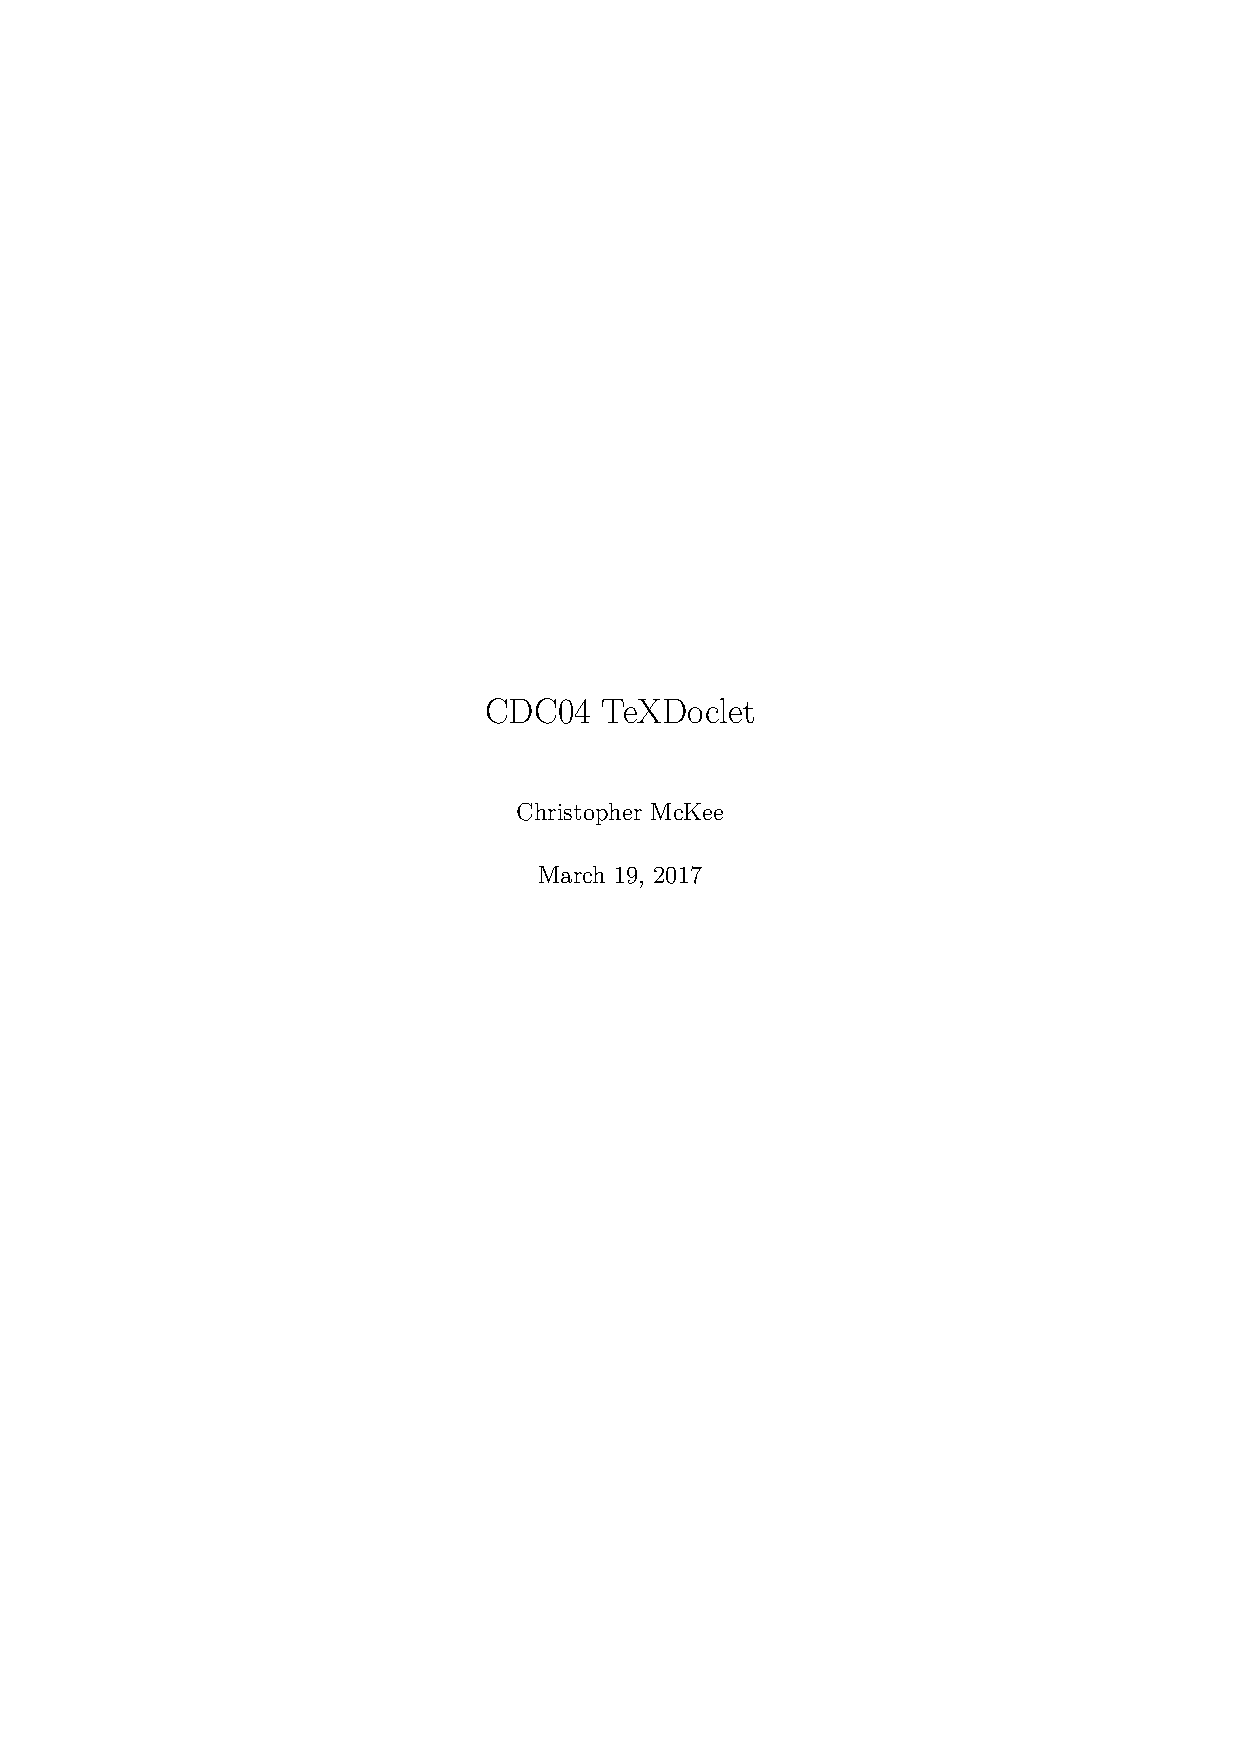
\includepdf[pages=-]{javadoc.pdf}
\end{document}
\end